%&preformat-disser
\RequirePackage[l2tabu,orthodox]{nag} % Раскомментировав, можно в логе получать рекомендации относительно правильного использования пакетов и предупреждения об устаревших и нерекомендуемых пакетах
% Формат А4, 14pt (ГОСТ Р 7.0.11-2011, 5.3.6)
\documentclass[a4paper,14pt,oneside,openany]{memoir}

%%%%%%%%%%%%%%%%%%%%%%%%%%%%%%%%%%%%%%%%%%%%%%%%%%%%%%%
%%%% Файл упрощённых настроек шаблона автореферата %%%%
%%%%%%%%%%%%%%%%%%%%%%%%%%%%%%%%%%%%%%%%%%%%%%%%%%%%%%%

%%% Инициализирование переменных, не трогать!  %%%
\newcounter{showperssign}
\newcounter{showsecrsign}
\newcounter{showopplead}
%%%%%%%%%%%%%%%%%%%%%%%%%%%%%%%%%%%%%%%%%%%%%%%%%%%%%%%

%%% Список публикаций %%%
\makeatletter
\@ifundefined{c@usefootcite}{
  \newcounter{usefootcite}
  \setcounter{usefootcite}{0} % 0 --- два списка литературы;
                              % 1 --- список публикаций автора + цитирование
                              %       других работ в сносках
}{}
\makeatother

\makeatletter
\@ifundefined{c@bibgrouped}{
  \newcounter{bibgrouped}
  \setcounter{bibgrouped}{1}  % 0 --- единый список работ автора;
                              % 1 --- сгруппированные работы автора
}{}
\makeatother

%%% Область упрощённого управления оформлением %%%

%% Управление зазором между подрисуночной подписью и основным текстом %%
\setlength{\belowcaptionskip}{10pt plus 20pt minus 2pt}


%% Подпись таблиц %%

% смещение строк подписи после первой
%\newcommand{\tabindent}{0cm}

% тип форматирования таблицы
% plain --- название и текст в одной строке
% split --- название и текст в разных строках
%\newcommand{\tabformat}{plain}

%%% настройки форматирования таблицы `plain'

% выравнивание по центру подписи, состоящей из одной строки
% true  --- выравнивать
% false --- не выравнивать
%\newcommand{\tabsinglecenter}{false}

% выравнивание подписи таблиц
% justified   --- выравнивать как обычный текст
% centering   --- выравнивать по центру
% centerlast  --- выравнивать по центру только последнюю строку
% centerfirst --- выравнивать по центру только первую строку
% raggedleft  --- выравнивать по правому краю
% raggedright --- выравнивать по левому краю
%\newcommand{\tabjust}{justified}

% Разделитель записи «Таблица #» и названия таблицы
%\newcommand{\tablabelsep}{~\cyrdash\ }

%%% настройки форматирования таблицы `split'

% положение названия таблицы
% \centering   --- выравнивать по центру
% \raggedleft  --- выравнивать по правому краю
% \raggedright --- выравнивать по левому краю
%\newcommand{\splitformatlabel}{\raggedleft}

% положение текста подписи
% \centering   --- выравнивать по центру
% \raggedleft  --- выравнивать по правому краю
% \raggedright --- выравнивать по левому краю
%\newcommand{\splitformattext}{\raggedright}

%% Подпись рисунков %%
%Разделитель записи «Рисунок #» и названия рисунка
%\newcommand{\fisglabelsep}{~\cyrdash\ }  % (ГОСТ 2.105, 4.3.1)
                                        % "--- здесь не работает

%Демонстрация подписи диссертанта на автореферате
\setcounter{showperssign}{1}  % 0 --- не показывать;
                              % 1 --- показывать
%Демонстрация подписи учёного секретаря на автореферате
\setcounter{showsecrsign}{1}  % 0 --- не показывать;
                              % 1 --- показывать
%Демонстрация информации об оппонентах и ведущей организации на автореферате
\setcounter{showopplead}{1}   % 0 --- не показывать;
                              % 1 --- показывать

%%% Цвета гиперссылок %%%
% Latex color definitions: http://latexcolor.com/
%\definecolor{linkcolor}{rgb}{0.9,0,0}
%\definecolor{citecolor}{rgb}{0,0.6,0}
%\definecolor{urlcolor}{rgb}{0,0,1}
\definecolor{linkcolor}{rgb}{0,0,0} %black
\definecolor{citecolor}{rgb}{0,0,0} %black
\definecolor{urlcolor}{rgb}{0,0,0} %black
            % общие настройки шаблона
%%% Проверка используемого TeX-движка %%%
\newif\ifxetexorluatex   % определяем новый условный оператор (http://tex.stackexchange.com/a/47579)
\ifxetex
    \xetexorluatextrue
\else
    \ifluatex
        \xetexorluatextrue
    \else
        \xetexorluatexfalse
    \fi
\fi

\newif\ifsynopsis           % Условие, проверяющее, что документ --- автореферат

\usepackage{etoolbox}[2015/08/02]   % Для продвинутой проверки разных условий
\providebool{presentation}

\usepackage{comment}    % Позволяет убирать блоки текста (добавляет
                        % окружение comment и команду \excludecomment)

%%% Поля и разметка страницы %%%
\usepackage{pdflscape}  % Для включения альбомных страниц
\usepackage{geometry}   % Для последующего задания полей

%%% Математические пакеты %%%
\usepackage{amsthm,amsmath,amscd}   % Математические дополнения от AMS
\usepackage{amsfonts,amssymb}       % Математические дополнения от AMS
\usepackage{mathtools}              % Добавляет окружение multlined
\usepackage{xfrac}                  % Красивые дроби
\usepackage[
    locale = DE,
    list-separator       = {;\,},
    list-final-separator = {;\,},
    list-pair-separator  = {;\,},
    list-units           = single,
    range-units          = single,
    range-phrase={\text{\ensuremath{-}}},
    % quotient-mode        = fraction, % красивые дроби могут не соответствовать ГОСТ
    fraction-function    = \sfrac,
    separate-uncertainty,
    ]{siunitx}                      % Размерности SI
\sisetup{inter-unit-product = \ensuremath{{}\cdot{}}}

% Кириллица в нумерации subequations
% Для правильной работы требуется выполнение сразу после загрузки пакетов
\patchcmd{\subequations}{\def\theequation{\theparentequation\alph{equation}}}
{\def\theequation{\theparentequation\asbuk{equation}}}
{\typeout{subequations patched}}{\typeout{subequations not patched}}

%%%% Установки для размера шрифта 14 pt %%%%
%% Формирование переменных и констант для сравнения (один раз для всех подключаемых файлов)%%
%% должно располагаться до вызова пакета fontspec или polyglossia, потому что они сбивают его работу
\newlength{\curtextsize}
\newlength{\bigtextsize}
\setlength{\bigtextsize}{13.9pt}

\makeatletter
%\show\f@size    % неплохо для отслеживания, но вызывает стопорение процесса,
                 % если документ компилируется без команды  -interaction=nonstopmode
\setlength{\curtextsize}{\f@size pt}
\makeatother

%%% Кодировки и шрифты %%%
\ifxetexorluatex
    \ifpresentation
        \providecommand*\autodot{} % quick fix for polyglossia 1.50
    \fi
    \PassOptionsToPackage{no-math}{fontspec}    % https://tex.stackexchange.com/a/26295/104425
    \usepackage{polyglossia}[2014/05/21]        % Поддержка многоязычности
                                        % (fontspec подгружается автоматически)
\else
   %%% Решение проблемы копирования текста в буфер кракозябрами
    \ifnumequal{\value{usealtfont}}{0}{}{
        \input glyphtounicode.tex
        \input glyphtounicode-cmr.tex %from pdfx package
        \pdfgentounicode=1
    }
    \usepackage{cmap}   % Улучшенный поиск русских слов в полученном pdf-файле
    \ifnumequal{\value{usealtfont}}{2}{}{
        \defaulthyphenchar=127  % Если стоит до fontenc, то переносы
                                % не впишутся в выделяемый текст при
                                % копировании его в буфер обмена
    }
    \usepackage{textcomp}
    \usepackage[T1,T2A]{fontenc}                    % Поддержка русских букв
    \ifnumequal{\value{usealtfont}}{1}{% Используется pscyr, при наличии
        \IfFileExists{pscyr.sty}{\usepackage{pscyr}}{}  % Подключение pscyr
    }{}
    \usepackage[utf8]{inputenc}[2014/04/30]         % Кодировка utf8
    \usepackage[english, russian]{babel}[2014/03/24]% Языки: русский, английский
    \makeatletter\AtBeginDocument{\let\@elt\relax}\makeatother % babel 3.40 fix
    \ifnumequal{\value{usealtfont}}{2}{
        % http://dxdy.ru/post1238763.html#p1238763
        \usepackage[scaled=0.914]{XCharter}[2017/12/19] % Подключение русифицированных шрифтов XCharter
        \usepackage[charter, vvarbb, scaled=1.048]{newtxmath}[2017/12/14]
        \ifpresentation
        \else
            \setDisplayskipStretch{-0.078}
        \fi
    }{}
\fi

%%% Оформление абзацев %%%
\ifpresentation
\else
    \indentafterchapter     % Красная строка после заголовков типа chapter
    \usepackage{indentfirst}
\fi

%%% Цвета %%%
\ifpresentation
\else
    \usepackage[dvipsnames, table, hyperref]{xcolor} % Совместимо с tikz
\fi

%%% Таблицы %%%
\usepackage{longtable,ltcaption} % Длинные таблицы
\usepackage{multirow,makecell}   % Улучшенное форматирование таблиц
\usepackage{tabu, tabulary}      % таблицы с автоматически подбирающейся
                                 % шириной столбцов (tabu обязательно
                                 % до hyperref вызывать)
\usepackage{threeparttable}      % автоматический подгон ширины подписи таблицы

%%% Общее форматирование
\usepackage{soulutf8}% Поддержка переносоустойчивых подчёркиваний и зачёркиваний
\usepackage{icomma}  % Запятая в десятичных дробях

%%% Оптимизация расстановки переносов и длины последней строки абзаца
\IfFileExists{impnattypo.sty}{% проверка установленности пакета impnattypo
    \ifluatex
        \ifnumequal{\value{draft}}{1}{% Черновик
            \usepackage[hyphenation, lastparline, nosingleletter, homeoarchy,
            rivers, draft]{impnattypo}
        }{% Чистовик
            \usepackage[hyphenation, lastparline, nosingleletter]{impnattypo}
        }
    \else
        \usepackage[hyphenation, lastparline]{impnattypo}
    \fi
}{}

%% Векторная графика

\usepackage{tikz}                   % Продвинутый пакет векторной графики
\usetikzlibrary{chains}             % Для примера tikz рисунка
\usetikzlibrary{shapes.geometric}   % Для примера tikz рисунка
\usetikzlibrary{shapes.symbols}     % Для примера tikz рисунка
\usetikzlibrary{arrows}             % Для примера tikz рисунка

%%% Гиперссылки %%%
\usepackage{hyperref}[2012/11/06]

%%% Изображения %%%
\usepackage{graphicx}[2014/04/25]   % Подключаем пакет работы с графикой
\usepackage{caption}                % Подписи рисунков и таблиц
\usepackage{subcaption}             % Подписи подрисунков и подтаблиц
\usepackage{pdfpages}               % Добавление внешних pdf файлов

%%% Счётчики %%%
\usepackage{aliascnt}
\usepackage[figure,table]{totalcount}   % Счётчик рисунков и таблиц
\usepackage{totcount}   % Пакет создания счётчиков на основе последнего номера
                        % подсчитываемого элемента (может требовать дважды
                        % компилировать документ)
\usepackage{totpages}   % Счётчик страниц, совместимый с hyperref (ссылается
                        % на номер последней страницы). Желательно ставить
                        % последним пакетом в преамбуле

%%% Продвинутое управление групповыми ссылками (пока только формулами) %%%
\ifpresentation
\else
    \usepackage[russian]{cleveref} % cleveref имеет сложности со считыванием
    % языка из babel. Такое решение русификации вывода выбрано вместо
    % определения в documentclass из опасности что-то лишнее передать во все
    % остальные пакеты, включая библиографию.

    % Добавление возможности использования пробелов в \labelcref
    % https://tex.stackexchange.com/a/340502/104425
    \usepackage{kvsetkeys}
    \makeatletter
    \let\org@@cref\@cref
    \renewcommand*{\@cref}[2]{%
        \edef\process@me{%
            \noexpand\org@@cref{#1}{\zap@space#2 \@empty}%
        }\process@me
    }
    \makeatother
\fi

\usepackage{placeins} % для \FloatBarrier

\ifnumequal{\value{draft}}{1}{% Черновик
    \usepackage[firstpage]{draftwatermark}
    \SetWatermarkText{DRAFT}
    \SetWatermarkFontSize{14pt}
    \SetWatermarkScale{15}
    \SetWatermarkAngle{45}
}{}

%%% Цитата, не приводимая в автореферате:
% возможно, актуальна только для biblatex
%\newcommand{\citeinsynopsis}[1]{\ifsynopsis\else ~\cite{#1} \fi}

% если текущий процесс запущен библиотекой tikz-external, то прекомпиляция должна быть включена
\ifdefined\tikzexternalrealjob
    \setcounter{imgprecompile}{1}
\fi

\ifnumequal{\value{imgprecompile}}{1}{% Только если у нас включена предкомпиляция
    \usetikzlibrary{external}   % подключение возможности предкомпиляции
    \tikzexternalize[prefix=images/cache/,optimize command away=\includepdf] % activate! % здесь можно указать отдельную папку для скомпилированных файлов
    \ifxetex
        \tikzset{external/up to date check={diff}}
    \fi
}{}         % Пакеты общие для диссертации и автореферата
\synopsisfalse                      % Этот документ --- не автореферат
\input{Dissertation/dispackages}    % Пакеты для диссертации
\usepackage{fr-longtable}    %ради \endlasthead

% Листинги с исходным кодом программ
\usepackage{fancyvrb}
\usepackage{listings}
\lccode`\~=0\relax %Без этого хака из-за особенностей пакета listings перестают работать конструкции с \MakeLowercase и т. п. в (xe|lua)latex

% Русская традиция начертания греческих букв
\usepackage{upgreek} % прямые греческие ради русской традиции
\usepackage{tabularx}

%%% Микротипографика
%\ifnumequal{\value{draft}}{0}{% Только если у нас режим чистовика
%    \usepackage[final, babel, shrink=45]{microtype}[2016/05/14] % улучшает представление букв и слов в строках, может помочь при наличии отдельно висящих слов
%}{}

\usepackage{IEEEtrantools}

% Отметка о версии черновика на каждой странице
% Чтобы работало надо в своей локальной копии по инструкции
% https://www.ctan.org/pkg/gitinfo2 создать небходимые файлы в папке
% ./git/hooks
% If you’re familiar with tweaking git, you can probably work it out for
% yourself. If not, I suggest you follow these steps:
% 1. First, you need a git repository and working tree. For this example,
% let’s suppose that the root of the working tree is in ~/compsci
% 2. Copy the file post-xxx-sample.txt (which is in the same folder of
% your TEX distribution as this pdf) into the git hooks directory in your
% working copy. In our example case, you should end up with a file called
% ~/compsci/.git/hooks/post-checkout
% 3. If you’re using a unix-like system, don’t forget to make the file executable.
% Just how you do this is outside the scope of this manual, but one
% possible way is with commands such as this:
% chmod g+x post-checkout.
% 4. Test your setup with “git checkout master” (or another suitable branch
% name). This should generate copies of gitHeadInfo.gin in the directories
% you intended.
% 5. Now make two more copies of this file in the same directory (hooks),
% calling them post-commit and post-merge, and you’re done. As before,
% users of unix-like systems should ensure these files are marked as
% executable.
\ifnumequal{\value{draft}}{1}{% Черновик
   \IfFileExists{.git/gitHeadInfo.gin}{
      \usepackage[mark,pcount]{gitinfo2}
      \renewcommand{\gitMark}{rev.\gitAbbrevHash\quad\gitCommitterEmail\quad\gitAuthorIsoDate}
      \renewcommand{\gitMarkFormat}{\rmfamily\color{Gray}\small\bfseries}
   }{}
}{}   % Пакеты для специфических пользовательских задач

%%%%%%%%%%%%%%%%%%%%%%%%%%%%%%%%%%%%%%%%%%%%%%%%%%%%%%
%%%% Файл упрощённых настроек шаблона диссертации %%%%
%%%%%%%%%%%%%%%%%%%%%%%%%%%%%%%%%%%%%%%%%%%%%%%%%%%%%%

%%% Инициализирование переменных, не трогать!  %%%
\newcounter{intvl}
\newcounter{otstup}
\newcounter{contnumeq}
\newcounter{contnumfig}
\newcounter{contnumtab}
\newcounter{pgnum}
\newcounter{chapstyle}
\newcounter{headingdelim}
\newcounter{headingalign}
\newcounter{headingsize}
%%%%%%%%%%%%%%%%%%%%%%%%%%%%%%%%%%%%%%%%%%%%%%%%%%%%%%

%%% Область упрощённого управления оформлением %%%

%% Интервал между заголовками и между заголовком и текстом %%
% Заголовки отделяют от текста сверху и снизу
% тремя интервалами (ГОСТ Р 7.0.11-2011, 5.3.5)
\setcounter{intvl}{3}               % Коэффициент кратности к размеру шрифта

%% Отступы у заголовков в тексте %%
\setcounter{otstup}{0}              % 0 --- без отступа; 1 --- абзацный отступ

%% Нумерация формул, таблиц и рисунков %%
% Нумерация формул
\setcounter{contnumeq}{0}   % 0 --- пораздельно (во введении подряд,
                            %       без номера раздела);
                            % 1 --- сквозная нумерация по всей диссертации
% Нумерация рисунков
\setcounter{contnumfig}{0}  % 0 --- пораздельно (во введении подряд,
                            %       без номера раздела);
                            % 1 --- сквозная нумерация по всей диссертации
% Нумерация таблиц
\setcounter{contnumtab}{1}  % 0 --- пораздельно (во введении подряд,
                            %       без номера раздела);
                            % 1 --- сквозная нумерация по всей диссертации

%% Оглавление %%
\setcounter{pgnum}{1}       % 0 --- номера страниц никак не обозначены;
                            % 1 --- Стр. над номерами страниц (дважды
                            %       компилировать после изменения настройки)
\settocdepth{subsection}    % до какого уровня подразделов выносить в оглавление
\setsecnumdepth{subsection} % до какого уровня нумеровать подразделы


%% Текст и форматирование заголовков %%
\setcounter{chapstyle}{1}     % 0 --- разделы только под номером;
                              % 1 --- разделы с названием "Глава" перед номером
\setcounter{headingdelim}{1}  % 0 --- номер отделен пропуском в 1em или \quad;
                              % 1 --- номера разделов и приложений отделены
                              %       точкой с пробелом, подразделы пропуском
                              %       без точки;
                              % 2 --- номера разделов, подразделов и приложений
                              %       отделены точкой с пробелом.

%% Выравнивание заголовков в тексте %%
\setcounter{headingalign}{0}  % 0 --- по центру;
                              % 1 --- по левому краю

%% Размеры заголовков в тексте %%
\setcounter{headingsize}{0}   % 0 --- по ГОСТ, все всегда 14 пт;
                              % 1 --- пропорционально изменяющийся размер
                              %       в зависимости от базового шрифта

%% Подпись таблиц %%

% Смещение строк подписи после первой строки
\newcommand{\tabindent}{0cm}

% Тип форматирования заголовка таблицы:
% plain --- название и текст в одной строке
% split --- название и текст в разных строках
\newcommand{\tabformat}{plain}

%%% Настройки форматирования таблицы `plain`

% Выравнивание по центру подписи, состоящей из одной строки:
% true  --- выравнивать
% false --- не выравнивать
\newcommand{\tabsinglecenter}{false}

% Выравнивание подписи таблиц:
% justified   --- выравнивать как обычный текст («по ширине»)
% centering   --- выравнивать по центру
% centerlast  --- выравнивать по центру только последнюю строку
% centerfirst --- выравнивать по центру только первую строку (не рекомендуется)
% raggedleft  --- выравнивать по правому краю
% raggedright --- выравнивать по левому краю
\newcommand{\tabjust}{justified}

% Разделитель записи «Таблица #» и названия таблицы
\newcommand{\tablabelsep}{~\cyrdash\ }

%%% Настройки форматирования таблицы `split`

% Положение названия таблицы:
% \centering   --- выравнивать по центру
% \raggedleft  --- выравнивать по правому краю
% \raggedright --- выравнивать по левому краю
\newcommand{\splitformatlabel}{\raggedleft}

% Положение текста подписи:
% \centering   --- выравнивать по центру
% \raggedleft  --- выравнивать по правому краю
% \raggedright --- выравнивать по левому краю
\newcommand{\splitformattext}{\raggedright}

%% Подпись рисунков %%
%Разделитель записи «Рисунок #» и названия рисунка
\newcommand{\figlabelsep}{~\cyrdash\ }  % (ГОСТ 2.105, 4.3.1)
                                        % "--- здесь не работает

%%% Цвета гиперссылок %%%
% Latex color definitions: http://latexcolor.com/
%\definecolor{linkcolor}{rgb}{0.9,0,0}
%\definecolor{citecolor}{rgb}{0,0.6,0}
%\definecolor{urlcolor}{rgb}{0,0,1}
\definecolor{linkcolor}{rgb}{0,0,0} %black
\definecolor{citecolor}{rgb}{0,0,0} %black
\definecolor{urlcolor}{rgb}{0,0,0} %black
      % Упрощённые настройки шаблона

% Новые переменные, которые могут использоваться во всём проекте
% ГОСТ 7.0.11-2011
% 9.2 Оформление текста автореферата диссертации
% 9.2.1 Общая характеристика работы включает в себя следующие основные структурные
% элементы:
% актуальность темы исследования;
\newcommand{\actualityTXT}{Актуальность темы.}
\newcommand{\actualityTXTEn}{Relevance.}
% степень ее разработанности;
\newcommand{\progressTXT}{Степень разработанности темы.}
\newcommand{\progressTXTEn}{State of the field.}
% цели и задачи;
\newcommand{\aimTXT}{Целью}
\newcommand{\aimTXTEn}{The aim}
\newcommand{\tasksTXT}{задачи}
\newcommand{\tasksTXTEn}{tasks}
% научную новизну;
\newcommand{\noveltyTXT}{Научная новизна:}
\newcommand{\noveltyTXTEn}{The scientific novelty:}
% теоретическую и практическую значимость работы;
%\newcommand{\influenceTXT}{Теоретическая и практическая значимость}
% или чаще используют просто
\newcommand{\influenceTXT}{Практическая значимость}
\newcommand{\influenceTXTEn}{The practical significance}
% методологию и методы исследования;
\newcommand{\methodsTXT}{Методология и методы исследования.}
\newcommand{\methodsTXTEn}{Study methodology and methods.}
% положения, выносимые на защиту;
\newcommand{\defpositionsTXT}{Основные положения, выносимые на~защиту:}
\newcommand{\defpositionsTXTEn}{The principal statements of the~thesis:}
% степень достоверности и апробацию результатов.
\newcommand{\reliabilityTXT}{Достоверность}
\newcommand{\reliabilityTXTEn}{The validity and reliability}
\newcommand{\probationTXT}{Апробация работы.}
\newcommand{\probationTXTEn}{Approbation.}

\newcommand{\contributionTXT}{Личный вклад.}
\newcommand{\contributionTXTEn}{Personal contribution.}
\newcommand{\implementationTXT}{Внедрение результатов работы.}
\newcommand{\implementationTXTEn}{Application.}
\newcommand{\publicationsTXT}{Публикации.}
\newcommand{\publicationsTXTEn}{Publications.}

%%% Заголовки библиографии:

% для автореферата:
\newcommand{\bibtitleauthor}{Публикации автора по теме диссертации}
\newcommand{\bibtitleauthorEn}{List of own publications}

% для стиля библиографии `\insertbiblioauthorgrouped`
\newcommand{\bibtitleauthorvak}{В изданиях из списка ВАК РФ}
\newcommand{\bibtitleauthorvakEn}{Publications in editions from the list of the Higher Attestation Commission}


\newcommand{\bibtitleauthorscopus}{В изданиях, входящих в международную базы цитирования Scopus и Web of Science}
\newcommand{\bibtitleauthorscopusEn}{Publications in international editions, indexed in Scopus and WoS}

\newcommand{\bibtitleauthorwos}{В изданиях, входящих в международную базу цитирования Web of Science}

\newcommand{\bibtitleauthorother}{В прочих изданиях}
\newcommand{\bibtitleauthorotherEn}{In other editions}

\newcommand{\bibtitleauthorconf}{В сборниках трудов конференций}
\newcommand{\bibtitleauthorpatent}{Зарегистрированные патенты}
\newcommand{\bibtitleauthorprogram}{Зарегистрированные программы для ЭВМ}

% для стиля библиографии `\insertbiblioauthorimportant`:
\newcommand{\bibtitleauthorimportant}{Наиболее значимые \protect\MakeLowercase\bibtitleauthor}

% для списка литературы в диссертации и списка чужих работ в автореферате:
\newcommand{\bibtitlefull}{Список литературы} % (ГОСТ Р 7.0.11-2011, 4)
         % Новые переменные, для всего проекта

%%% Основные сведения %%%
\newcommand{\thesisAuthorLastName}{Крылова}
\newcommand{\thesisAuthorOtherNames}{Анастасия Андреевна}
\newcommand{\thesisAuthorLastNameEn}{Krylova}
\newcommand{\thesisAuthorOtherNamesEn}{Anastasiya Andreevna}
\newcommand{\thesisAuthorInitials}{А.\,А.}
\newcommand{\thesisAuthorEn}{\thesisAuthorLastNameEn~\thesisAuthorOtherNamesEn}
\newcommand{\thesisAuthor}             % Диссертация, ФИО автора
{%
    \texorpdfstring{% \texorpdfstring takes two arguments and uses the first for (La)TeX and the second for pdf
        \thesisAuthorLastName~\thesisAuthorOtherNames% так будет отображаться на титульном листе или в тексте, где будет использоваться переменная
    }{%
        \thesisAuthorLastName, \thesisAuthorOtherNames% эта запись для свойств pdf-файла. В таком виде, если pdf будет обработан программами для сбора библиографических сведений, будет правильно представлена фамилия.
    }
}
\newcommand{\thesisAuthorShort}        % Диссертация, ФИО автора инициалами
{\thesisAuthorInitials~\thesisAuthorLastName}
%\newcommand{\thesisUdk}                % Диссертация, УДК
%{\fixme{xxx.xxx}}
\newcommand{\thesisTitle}              % Диссертация, название
{Исследование и~разработка модульного технологического оборудования для единичного и~мелкосерийного производства}
\newcommand{\thesisTitleEn}
{Research and Development of Modular Technological Equipment for Job and Small-batch production}
\newcommand{\thesisSpecialtyNumber}    % Диссертация, специальность, номер
{05.11.14}
\newcommand{\thesisSpecialtyTitle}     % Диссертация, специальность, название (название взято с сайта ВАК для примера)
{Технология приборостроения}
\newcommand{\thesisSpecialtyTitleEn}
{Instrumentation technology}
%% \newcommand{\thesisSpecialtyTwoNumber} % Диссертация, вторая специальность, номер
%% {\fixme{XX.XX.XX}}
%% \newcommand{\thesisSpecialtyTwoTitle}  % Диссертация, вторая специальность, название
%% {\fixme{Теория и~методика физического воспитания, спортивной тренировки,
%% оздоровительной и~адаптивной физической культуры}}
\newcommand{\thesisDegree}             % Диссертация, ученая степень
{кандидата технических наук}
\newcommand{\thesisDegreeEn}
{сandidate of engineering}
\newcommand{\thesisDegreeShort}        % Диссертация, ученая степень, краткая запись
{канд. техн. наук}
\newcommand{\thesisCity}               % Диссертация, город написания диссертации
{Санкт-Петербург}
\newcommand{\thesisCityEn}
{Saint-Petersburg}
\newcommand{\thesisYear}               % Диссертация, год написания диссертации
{\the\year}
\newcommand{\thesisOrganization}       % Диссертация, организация
{Национальный исследовательский университет ИТМО\\(Университет ИТМО)}
\newcommand{\thesisOrganizationEn}
{ITMO University}
\newcommand{\thesisOrganizationShort}  % Диссертация, краткое название организации для доклада
{Университет ИТМО}

\newcommand{\thesisInOrganization}     % Диссертация, организация в предложном падеже: Работа выполнена в ...
{федеральном государственном автономном образовательном учреждении высшего образования <<Национальный исследовательский университет ИТМО>>}

%% \newcommand{\supervisorDead}{}           % Рисовать рамку вокруг фамилии
\newcommand{\supervisorFio}              % Научный руководитель, ФИО
{Афанасьев Максим Яковлевич}
\newcommand{\supervisorFioEn}              % Научный руководитель, ФИО
{Afanasev Maksim Ya.}
\newcommand{\supervisorRegalia}          % Научный руководитель, регалии
{кандидат технических наук}
\newcommand{\supervisorRegaliaEn}
{candidate of engineering sciences}
\newcommand{\supervisorFioShort}         % Научный руководитель, ФИО
{М.\,Я.~Афанасьв}
\newcommand{\supervisorRegaliaShort}     % Научный руководитель, регалии
{к.\,т.\,н.}

%% \newcommand{\supervisorTwoDead}{}        % Рисовать рамку вокруг фамилии
%% \newcommand{\supervisorTwoFio}           % Второй научный руководитель, ФИО
%% {\fixme{Фамилия Имя Отчество}}
%% \newcommand{\supervisorTwoRegalia}       % Второй научный руководитель, регалии
%% {\fixme{уч. степень, уч. звание}}
%% \newcommand{\supervisorTwoFioShort}      % Второй научный руководитель, ФИО
%% {\fixme{И.\,О.~Фамилия}}
%% \newcommand{\supervisorTwoRegaliaShort}  % Второй научный руководитель, регалии
%% {\fixme{уч.~ст.,~уч.~зв.}}

\newcommand{\opponentOneFio}           % Оппонент 1, ФИО
{\fixme{Фамилия Имя Отчество}}
\newcommand{\opponentOneFioEn}
{\fixme{Surname Name Patronimic}}
%
\newcommand{\opponentOneRegalia}       % Оппонент 1, регалии
{\fixme{доктор физико-математических наук, профессор}}
\newcommand{\opponentOneRegaliaEn}      
{\fixme{Doctor of Technical Sciences, Professor}}
%
\newcommand{\opponentOneJobPlace}      % Оппонент 1, место работы
{\fixme{Не очень длинное название для места работы}}
\newcommand{\opponentOneJobPlaceEn}      
{\fixme{Place of work}}
%
\newcommand{\opponentOneJobPost}       % Оппонент 1, должность
{\fixme{старший научный сотрудник}}
\newcommand{\opponentOneJobPostEn}
{\fixme{position}}
%
\newcommand{\opponentTwoFio}           % Оппонент 2, ФИО
{\fixme{Фамилия Имя Отчество}}
\newcommand{\opponentTwoFioEn}
{\fixme{Surname Name Patronimic}}
%
\newcommand{\opponentTwoRegalia}       % Оппонент 2, регалии
{\fixme{кандидат технических наук}}
\newcommand{\opponentTwoRegaliaEn}
{\fixme{Doctor of Technical Sciences, Professor}}
%
\newcommand{\opponentTwoJobPlace}      % Оппонент 2, место работы
{\fixme{Основное место работы c длинным длинным длинным длинным названием}}
\newcommand{\opponentTwoJobPlaceEn}
{\fixme{Place of work}}
%
\newcommand{\opponentTwoJobPost}       % Оппонент 2, должность
{\fixme{старший научный сотрудник}}
\newcommand{\opponentTwoJobPostEn}
{\fixme{position}}

%% \newcommand{\opponentThreeFio}         % Оппонент 3, ФИО
%% {\fixme{Фамилия Имя Отчество}}
%% \newcommand{\opponentThreeRegalia}     % Оппонент 3, регалии
%% {\fixme{кандидат физико-математических наук}}
%% \newcommand{\opponentThreeJobPlace}    % Оппонент 3, место работы
%% {\fixme{Основное место работы c длинным длинным длинным длинным названием}}
%% \newcommand{\opponentThreeJobPost}     % Оппонент 3, должность
%% {\fixme{старший научный сотрудник}}

\newcommand{\leadingOrganizationTitle} % Ведущая организация, дополнительные строки. Удалить, чтобы не отображать в автореферате
{\fixme{Федеральное государственное бюджетное образовательное учреждение высшего
профессионального образования с~длинным длинным длинным длинным названием}}

\newcommand{\defenseDate}              % Защита, дата
{\fixme{DD.MM.YYYY~г.~в~XX:00 часов}}
\newcommand{\defenseDateEn}
{\fixme{DD.MM.YYYY at XX:00}}
\newcommand{\defenseCouncilNumber}     % Защита, номер диссертационного совета
{11.21.00}
\newcommand{\defenseCouncilTitle}      % Защита, учреждение диссертационного совета
{Университета ИТМО}
\newcommand{\defenseCouncilAddress}    % Защита, адрес учреждение диссертационного совета
{Санкт-Петербург, Кронверкский пр.\,49, лит.\,А, ауд.~\fixme{XXX}}
\newcommand{\defenseCouncilPhone}      % Телефон для справок
{\fixme{+7~(0000)~00-00-00}}

\newcommand{\defenseSecretaryFio}      % Секретарь диссертационного совета, ФИО
{Андреев Юрий Сергеевич}
\newcommand{\defenseSecretaryFioEn}
{Andreev IUrii Sergeevich}
\newcommand{\defenseSecretaryRegalia}  % Секретарь диссертационного совета, регалии
{кандидат технических наук}  % Для сокращений есть ГОСТы, например: ГОСТ Р 7.0.12-2011 + http://base.garant.ru/179724/#block_30000
\newcommand{\defenseSecretaryRegaliaEn}
{Candidate of Technical Sciences}

\newcommand{\synopsisLibrary}          % Автореферат, название библиотеки
{Универcитета ИТМО  по адресу: 197101, Санкт-Петербург, Кронверкский~пр., д.\,49, лит.\,А и на сайте \mbox{\url{https://dissovet.itmo.ru}}}
\newcommand{\synopsisLibraryEn}
{49 Kronversky pr., \mbox{Saint-Petersburg}, Russia and on \url{https://dissovet.itmo.ru} website}
\newcommand{\synopsisDate}             % Автореферат, дата рассылки
{\fixme{DD mmmmmmmm}\the\year~года}

% To avoid conflict with beamer class use \providecommand
\providecommand{\keywords}%            % Ключевые слова для метаданных PDF диссертации и автореферата
{}
             % Основные сведения
\input{common/fonts}            % Определение шрифтов (частичное)
%%% Шаблон %%%
\DeclareRobustCommand{\fixme}{\textcolor{red}}  % решаем проблему превращения
                                % названия цвета в результате \MakeUppercase,
                                % http://tex.stackexchange.com/a/187930,
                                % \DeclareRobustCommand protects \fixme
                                % from expanding inside \MakeUppercase
\AtBeginDocument{%
    \setlength{\parindent}{2.5em}                   % Абзацный отступ. Должен быть одинаковым по всему тексту и равен пяти знакам (ГОСТ Р 7.0.11-2011, 5.3.7).
}

%%% Таблицы %%%
\DeclareCaptionLabelSeparator{tabsep}{\tablabelsep} % нумерация таблиц
\DeclareCaptionFormat{split}{\splitformatlabel#1\par\splitformattext#3}

\captionsetup[table]{
        format=\tabformat,                % формат подписи (plain|hang)
        font=normal,                      % нормальные размер, цвет, стиль шрифта
        skip=.0pt,                        % отбивка под подписью
        parskip=.0pt,                     % отбивка между параграфами подписи
        position=above,                   % положение подписи
        justification=\tabjust,           % центровка
        indent=\tabindent,                % смещение строк после первой
        labelsep=tabsep,                  % разделитель
        singlelinecheck=\tabsinglecenter, % не выравнивать по центру, если умещается в одну строку
}

%%% Рисунки %%%
\DeclareCaptionLabelSeparator{figsep}{\figlabelsep} % нумерация рисунков

\captionsetup[figure]{
        format=plain,                     % формат подписи (plain|hang)
        font=normal,                      % нормальные размер, цвет, стиль шрифта
        skip=.0pt,                        % отбивка под подписью
        parskip=.0pt,                     % отбивка между параграфами подписи
        position=below,                   % положение подписи
        singlelinecheck=true,             % выравнивание по центру, если умещается в одну строку
        justification=centerlast,         % центровка
        labelsep=figsep,                  % разделитель
}

%%% Подписи подрисунков %%%
\DeclareCaptionSubType{figure}
\renewcommand\thesubfigure{\asbuk{subfigure}} % нумерация подрисунков
\ifsynopsis
\DeclareCaptionFont{norm}{\fontsize{10pt}{11pt}\selectfont}
\newcommand{\subfigureskip}{2.pt}
\else
\DeclareCaptionFont{norm}{\fontsize{14pt}{16pt}\selectfont}
\newcommand{\subfigureskip}{0.pt}
\fi

\captionsetup[subfloat]{
        labelfont=norm,                 % нормальный размер подписей подрисунков
        textfont=norm,                  % нормальный размер подписей подрисунков
        labelsep=space,                 % разделитель
        labelformat=brace,              % одна скобка справа от номера
        justification=centering,        % центровка
        singlelinecheck=true,           % выравнивание по центру, если умещается в одну строку
        skip=\subfigureskip,            % отбивка над подписью
        parskip=.0pt,                   % отбивка между параграфами подписи
        position=below,                 % положение подписи
}

%%% Настройки ссылок на рисунки, таблицы и др. %%%
% команды \cref...format отвечают за форматирование при помощи команды \cref
% команды \labelcref...format отвечают за форматирование при помощи команды \labelcref

\ifpresentation
\else
    \crefdefaultlabelformat{#2#1#3}

    % Уравнение
    \crefformat{equation}{(#2#1#3)} % одиночная ссылка с приставкой
    \labelcrefformat{equation}{(#2#1#3)} % одиночная ссылка без приставки
    \crefrangeformat{equation}{(#3#1#4) \cyrdash~(#5#2#6)} % диапазон ссылок с приставкой
    \labelcrefrangeformat{equation}{(#3#1#4) \cyrdash~(#5#2#6)} % диапазон ссылок без приставки
    \crefmultiformat{equation}{(#2#1#3)}{ и~(#2#1#3)}{, (#2#1#3)}{ и~(#2#1#3)} % перечисление ссылок с приставкой
    \labelcrefmultiformat{equation}{(#2#1#3)}{ и~(#2#1#3)}{, (#2#1#3)}{ и~(#2#1#3)} % перечисление без приставки

    % Подуравнение
    \crefformat{subequation}{(#2#1#3)} % одиночная ссылка с приставкой
    \labelcrefformat{subequation}{(#2#1#3)} % одиночная ссылка без приставки
    \crefrangeformat{subequation}{(#3#1#4) \cyrdash~(#5#2#6)} % диапазон ссылок с приставкой
    \labelcrefrangeformat{subequation}{(#3#1#4) \cyrdash~(#5#2#6)} % диапазон ссылок без приставки
    \crefmultiformat{subequation}{(#2#1#3)}{ и~(#2#1#3)}{, (#2#1#3)}{ и~(#2#1#3)} % перечисление ссылок с приставкой
    \labelcrefmultiformat{subequation}{(#2#1#3)}{ и~(#2#1#3)}{, (#2#1#3)}{ и~(#2#1#3)} % перечисление без приставки

    % Глава
    \crefformat{chapter}{#2#1#3} % одиночная ссылка с приставкой
    \labelcrefformat{chapter}{#2#1#3} % одиночная ссылка без приставки
    \crefrangeformat{chapter}{#3#1#4 \cyrdash~#5#2#6} % диапазон ссылок с приставкой
    \labelcrefrangeformat{chapter}{#3#1#4 \cyrdash~#5#2#6} % диапазон ссылок без приставки
    \crefmultiformat{chapter}{#2#1#3}{ и~#2#1#3}{, #2#1#3}{ и~#2#1#3} % перечисление ссылок с приставкой
    \labelcrefmultiformat{chapter}{#2#1#3}{ и~#2#1#3}{, #2#1#3}{ и~#2#1#3} % перечисление без приставки

    % Параграф
    \crefformat{section}{#2#1#3} % одиночная ссылка с приставкой
    \labelcrefformat{section}{#2#1#3} % одиночная ссылка без приставки
    \crefrangeformat{section}{#3#1#4 \cyrdash~#5#2#6} % диапазон ссылок с приставкой
    \labelcrefrangeformat{section}{#3#1#4 \cyrdash~#5#2#6} % диапазон ссылок без приставки
    \crefmultiformat{section}{#2#1#3}{ и~#2#1#3}{, #2#1#3}{ и~#2#1#3} % перечисление ссылок с приставкой
    \labelcrefmultiformat{section}{#2#1#3}{ и~#2#1#3}{, #2#1#3}{ и~#2#1#3} % перечисление без приставки

    % Приложение
    \crefformat{appendix}{#2#1#3} % одиночная ссылка с приставкой
    \labelcrefformat{appendix}{#2#1#3} % одиночная ссылка без приставки
    \crefrangeformat{appendix}{#3#1#4 \cyrdash~#5#2#6} % диапазон ссылок с приставкой
    \labelcrefrangeformat{appendix}{#3#1#4 \cyrdash~#5#2#6} % диапазон ссылок без приставки
    \crefmultiformat{appendix}{#2#1#3}{ и~#2#1#3}{, #2#1#3}{ и~#2#1#3} % перечисление ссылок с приставкой
    \labelcrefmultiformat{appendix}{#2#1#3}{ и~#2#1#3}{, #2#1#3}{ и~#2#1#3} % перечисление без приставки

    % Рисунок
    \crefformat{figure}{#2#1#3} % одиночная ссылка с приставкой
    \labelcrefformat{figure}{#2#1#3} % одиночная ссылка без приставки
    \crefrangeformat{figure}{#3#1#4 \cyrdash~#5#2#6} % диапазон ссылок с приставкой
    \labelcrefrangeformat{figure}{#3#1#4 \cyrdash~#5#2#6} % диапазон ссылок без приставки
    \crefmultiformat{figure}{#2#1#3}{ и~#2#1#3}{, #2#1#3}{ и~#2#1#3} % перечисление ссылок с приставкой
    \labelcrefmultiformat{figure}{#2#1#3}{ и~#2#1#3}{, #2#1#3}{ и~#2#1#3} % перечисление без приставки

    % Таблица
    \crefformat{table}{#2#1#3} % одиночная ссылка с приставкой
    \labelcrefformat{table}{#2#1#3} % одиночная ссылка без приставки
    \crefrangeformat{table}{#3#1#4 \cyrdash~#5#2#6} % диапазон ссылок с приставкой
    \labelcrefrangeformat{table}{#3#1#4 \cyrdash~#5#2#6} % диапазон ссылок без приставки
    \crefmultiformat{table}{#2#1#3}{ и~#2#1#3}{, #2#1#3}{ и~#2#1#3} % перечисление ссылок с приставкой
    \labelcrefmultiformat{table}{#2#1#3}{ и~#2#1#3}{, #2#1#3}{ и~#2#1#3} % перечисление без приставки

    % Листинг
    \crefformat{lstlisting}{#2#1#3} % одиночная ссылка с приставкой
    \labelcrefformat{lstlisting}{#2#1#3} % одиночная ссылка без приставки
    \crefrangeformat{lstlisting}{#3#1#4 \cyrdash~#5#2#6} % диапазон ссылок с приставкой
    \labelcrefrangeformat{lstlisting}{#3#1#4 \cyrdash~#5#2#6} % диапазон ссылок без приставки
    \crefmultiformat{lstlisting}{#2#1#3}{ и~#2#1#3}{, #2#1#3}{ и~#2#1#3} % перечисление ссылок с приставкой
    \labelcrefmultiformat{lstlisting}{#2#1#3}{ и~#2#1#3}{, #2#1#3}{ и~#2#1#3} % перечисление без приставки

    % Листинг
    \crefformat{ListingEnv}{#2#1#3} % одиночная ссылка с приставкой
    \labelcrefformat{ListingEnv}{#2#1#3} % одиночная ссылка без приставки
    \crefrangeformat{ListingEnv}{#3#1#4 \cyrdash~#5#2#6} % диапазон ссылок с приставкой
    \labelcrefrangeformat{ListingEnv}{#3#1#4 \cyrdash~#5#2#6} % диапазон ссылок без приставки
    \crefmultiformat{ListingEnv}{#2#1#3}{ и~#2#1#3}{, #2#1#3}{ и~#2#1#3} % перечисление ссылок с приставкой
    \labelcrefmultiformat{ListingEnv}{#2#1#3}{ и~#2#1#3}{, #2#1#3}{ и~#2#1#3} % перечисление без приставки
\fi

%%% Настройки гиперссылок %%%
\ifluatex
    \hypersetup{
        unicode,                % Unicode encoded PDF strings
    }
\fi

\hypersetup{
    linktocpage=true,           % ссылки с номера страницы в оглавлении, списке таблиц и списке рисунков
%    linktoc=all,                % both the section and page part are links
%    pdfpagelabels=false,        % set PDF page labels (true|false)
    plainpages=false,           % Forces page anchors to be named by the Arabic form  of the page number, rather than the formatted form
    colorlinks,                 % ссылки отображаются раскрашенным текстом, а не раскрашенным прямоугольником, вокруг текста
    linkcolor={linkcolor},      % цвет ссылок типа ref, eqref и подобных
    citecolor={citecolor},      % цвет ссылок-цитат
    urlcolor={urlcolor},        % цвет гиперссылок
%    hidelinks,                  % Hide links (removing color and border)
    pdftitle={\thesisTitle},    % Заголовок
    pdfauthor={\thesisAuthor},  % Автор
    pdfsubject={\thesisSpecialtyNumber\ \thesisSpecialtyTitle},      % Тема
%    pdfcreator={Создатель},     % Создатель, Приложение
%    pdfproducer={Производитель},% Производитель, Производитель PDF
    pdfkeywords={\keywords},    % Ключевые слова
    pdflang={ru},
}
\ifnumequal{\value{draft}}{1}{% Черновик
    \hypersetup{
        draft,
    }
}{}

%%% Списки %%%
% Используем короткое тире (endash) для ненумерованных списков (ГОСТ 2.105-95, пункт 4.1.7, требует дефиса, но так лучше смотрится)
\renewcommand{\labelitemi}{\normalfont\bfseries{--}}

% Перечисление строчными буквами латинского алфавита (ГОСТ 2.105-95, 4.1.7)
%\renewcommand{\theenumi}{\alph{enumi}}
%\renewcommand{\labelenumi}{\theenumi)}

% Перечисление строчными буквами русского алфавита (ГОСТ 2.105-95, 4.1.7)
\makeatletter
\AddEnumerateCounter{\asbuk}{\russian@alph}{щ}      % Управляем списками/перечислениями через пакет enumitem, а он 'не знает' про asbuk, потому 'учим' его
\makeatother
%\renewcommand{\theenumi}{\asbuk{enumi}} %первый уровень нумерации
%\renewcommand{\labelenumi}{\theenumi)} %первый уровень нумерации
\renewcommand{\theenumii}{\asbuk{enumii}} %второй уровень нумерации
\renewcommand{\labelenumii}{\theenumii)} %второй уровень нумерации
\renewcommand{\theenumiii}{\arabic{enumiii}} %третий уровень нумерации
\renewcommand{\labelenumiii}{\theenumiii)} %третий уровень нумерации

\setlist{nosep,%                                    % Единый стиль для всех списков (пакет enumitem), без дополнительных интервалов.
    labelindent=\parindent,leftmargin=*%            % Каждый пункт, подпункт и перечисление записывают с абзацного отступа (ГОСТ 2.105-95, 4.1.8)
}

%%% Правильная нумерация приложений, рисунков и формул %%%
%% По ГОСТ 2.105, п. 4.3.8 Приложения обозначают заглавными буквами русского алфавита,
%% начиная с А, за исключением букв Ё, З, Й, О, Ч, Ь, Ы, Ъ.
%% Здесь также переделаны все нумерации русскими буквами.
\ifxetexorluatex
    \makeatletter
    \def\russian@Alph#1{\ifcase#1\or
       А\or Б\or В\or Г\or Д\or Е\or Ж\or
       И\or К\or Л\or М\or Н\or
       П\or Р\or С\or Т\or У\or Ф\or Х\or
       Ц\or Ш\or Щ\or Э\or Ю\or Я\else\xpg@ill@value{#1}{russian@Alph}\fi}
    \def\russian@alph#1{\ifcase#1\or
       а\or б\or в\or г\or д\or е\or ж\or
       и\or к\or л\or м\or н\or
       п\or р\or с\or т\or у\or ф\or х\or
       ц\or ш\or щ\or э\or ю\or я\else\xpg@ill@value{#1}{russian@alph}\fi}
    \def\cyr@Alph#1{\ifcase#1\or
        А\or Б\or В\or Г\or Д\or Е\or Ж\or
        И\or К\or Л\or М\or Н\or
        П\or Р\or С\or Т\or У\or Ф\or Х\or
        Ц\or Ш\or Щ\or Э\or Ю\or Я\else\xpg@ill@value{#1}{cyr@Alph}\fi}
    \def\cyr@alph#1{\ifcase#1\or
        а\or б\or в\or г\or д\or е\or ж\or
        и\or к\or л\or м\or н\or
        п\or р\or с\or т\or у\or ф\or х\or
        ц\or ш\or щ\or э\or ю\or я\else\xpg@ill@value{#1}{cyr@alph}\fi}
    \makeatother
\else
    \makeatletter
    \if@uni@ode
      \def\russian@Alph#1{\ifcase#1\or
        А\or Б\or В\or Г\or Д\or Е\or Ж\or
        И\or К\or Л\or М\or Н\or
        П\or Р\or С\or Т\or У\or Ф\or Х\or
        Ц\or Ш\or Щ\or Э\or Ю\or Я\else\@ctrerr\fi}
    \else
      \def\russian@Alph#1{\ifcase#1\or
        \CYRA\or\CYRB\or\CYRV\or\CYRG\or\CYRD\or\CYRE\or\CYRZH\or
        \CYRI\or\CYRK\or\CYRL\or\CYRM\or\CYRN\or
        \CYRP\or\CYRR\or\CYRS\or\CYRT\or\CYRU\or\CYRF\or\CYRH\or
        \CYRC\or\CYRSH\or\CYRSHCH\or\CYREREV\or\CYRYU\or
        \CYRYA\else\@ctrerr\fi}
    \fi
    \if@uni@ode
      \def\russian@alph#1{\ifcase#1\or
        а\or б\or в\or г\or д\or е\or ж\or
        и\or к\or л\or м\or н\or
        п\or р\or с\or т\or у\or ф\or х\or
        ц\or ш\or щ\or э\or ю\or я\else\@ctrerr\fi}
    \else
      \def\russian@alph#1{\ifcase#1\or
        \cyra\or\cyrb\or\cyrv\or\cyrg\or\cyrd\or\cyre\or\cyrzh\or
        \cyri\or\cyrk\or\cyrl\or\cyrm\or\cyrn\or
        \cyrp\or\cyrr\or\cyrs\or\cyrt\or\cyru\or\cyrf\or\cyrh\or
        \cyrc\or\cyrsh\or\cyrshch\or\cyrerev\or\cyryu\or
        \cyrya\else\@ctrerr\fi}
    \fi
    \makeatother
\fi


%%http://www.linux.org.ru/forum/general/6993203#comment-6994589 (используется totcount)
\makeatletter
\def\formtotal#1#2#3#4#5{%
    \newcount\@c
    \@c\totvalue{#1}\relax
    \newcount\@last
    \newcount\@pnul
    \@last\@c\relax
    \divide\@last 10
    \@pnul\@last\relax
    \divide\@pnul 10
    \multiply\@pnul-10
    \advance\@pnul\@last
    \multiply\@last-10
    \advance\@last\@c
    #2%
    \ifnum\@pnul=1#5\else%
    \ifcase\@last#5\or#3\or#4\or#4\or#4\else#5\fi
    \fi
}
\makeatother

\newcommand{\formbytotal}[5]{\total{#1}~\formtotal{#1}{#2}{#3}{#4}{#5}}

%%% Команды рецензирования %%%
\ifboolexpr{ (test {\ifnumequal{\value{draft}}{1}}) or (test {\ifnumequal{\value{showmarkup}}{1}})}{
        \newrobustcmd{\todo}[1]{\textcolor{red}{#1}}
        \newrobustcmd{\note}[2][]{\ifstrempty{#1}{#2}{\textcolor{#1}{#2}}}
        \newenvironment{commentbox}[1][]%
        {\ifstrempty{#1}{}{\color{#1}}}%
        {}
}{
        \newrobustcmd{\todo}[1]{}
        \newrobustcmd{\note}[2][]{}
        \excludecomment{commentbox}
}


\hyphenation{ITMO}
\hyphenation{ИТМО}           % Стили общие для диссертации и автореферата
%%% Переопределение именований, если иначе не сработает %%%
%\gappto\captionsrussian{
%    \renewcommand{\chaptername}{Глава}
%    \renewcommand{\appendixname}{Приложение} % (ГОСТ Р 7.0.11-2011, 5.7)
%}

%%% Изображения %%%
\graphicspath{{images/}{Dissertation/images/}{Synopsis/images/}}         % Пути к изображениям

%%% Интервалы %%%
%% По ГОСТ Р 7.0.11-2011, пункту 5.3.6 требуется полуторный интервал
%% Реализация средствами класса (на основе setspace) ближе к типографской классике.
%% И правит сразу и в таблицах (если со звёздочкой)
%\DoubleSpacing*     % Двойной интервал
\OnehalfSpacing*    % Полуторный интервал
%\setSpacing{1.42}   % Полуторный интервал, подобный Ворду (возможно, стоит включать вместе с предыдущей строкой)

%%% Макет страницы %%%
% Выставляем значения полей (ГОСТ 7.0.11-2011, 5.3.7)
\geometry{a4paper, top=2cm, bottom=2cm, left=2.5cm, right=1cm, nofoot, nomarginpar} %, heightrounded, showframe
\setlength{\topskip}{0pt}   %размер дополнительного верхнего поля
\setlength{\footskip}{12.3pt} % снимет warning, согласно https://tex.stackexchange.com/a/334346

%%% Выравнивание и переносы %%%
%% http://tex.stackexchange.com/questions/241343/what-is-the-meaning-of-fussy-sloppy-emergencystretch-tolerance-hbadness
%% http://www.latex-community.org/forum/viewtopic.php?p=70342#p70342
\tolerance 1414
\hbadness 1414
\emergencystretch 1.5em % В случае проблем регулировать в первую очередь
\hfuzz 0.3pt
\vfuzz \hfuzz
%\raggedbottom
%\sloppy                 % Избавляемся от переполнений
\clubpenalty=10000      % Запрещаем разрыв страницы после первой строки абзаца
\widowpenalty=10000     % Запрещаем разрыв страницы после последней строки абзаца
\brokenpenalty=4991     % Ограничение на разрыв страницы, если строка заканчивается переносом

%%% Блок управления параметрами для выравнивания заголовков в тексте %%%
\newlength{\otstuplen}
\setlength{\otstuplen}{\theotstup\parindent}
\ifnumequal{\value{headingalign}}{0}{% выравнивание заголовков в тексте
    \newcommand{\hdngalign}{\centering}                % по центру
    \newcommand{\hdngaligni}{}% по центру
    \setlength{\otstuplen}{0pt}
}{%
    \newcommand{\hdngalign}{}                 % по левому краю
    \newcommand{\hdngaligni}{\hspace{\otstuplen}}      % по левому краю
} % В обоих случаях вроде бы без переноса, как и надо (ГОСТ Р 7.0.11-2011, 5.3.5)

%%% Оглавление %%%
\renewcommand{\cftchapterdotsep}{\cftdotsep}                % отбивка точками до номера страницы начала главы/раздела

%% Переносить слова в заголовке не допускается (ГОСТ Р 7.0.11-2011, 5.3.5). Заголовки в оглавлении должны точно повторять заголовки в тексте (ГОСТ Р 7.0.11-2011, 5.2.3). Прямого указания на запрет переносов в оглавлении нет, но по той же логике невнесения искажений в смысл, лучше в оглавлении не переносить:
\setrmarg{2.55em plus1fil}                             %To have the (sectional) titles in the ToC, etc., typeset ragged right with no hyphenation
\renewcommand{\cftchapterpagefont}{\normalfont}        % нежирные номера страниц у глав в оглавлении
\renewcommand{\cftchapterleader}{\cftdotfill{\cftchapterdotsep}}% нежирные точки до номеров страниц у глав в оглавлении
%\renewcommand{\cftchapterfont}{}                       % нежирные названия глав в оглавлении

\ifnumgreater{\value{headingdelim}}{0}{%
    \renewcommand\cftchapteraftersnum{.\space}       % добавляет точку с пробелом после номера раздела в оглавлении
}{}
\ifnumgreater{\value{headingdelim}}{1}{%
    \renewcommand\cftsectionaftersnum{.\space}       % добавляет точку с пробелом после номера подраздела в оглавлении
    \renewcommand\cftsubsectionaftersnum{.\space}    % добавляет точку с пробелом после номера подподраздела в оглавлении
    \renewcommand\cftsubsubsectionaftersnum{.\space} % добавляет точку с пробелом после номера подподподраздела в оглавлении
    \AfterEndPreamble{% без этого polyglossia сама всё переопределяет
        \setsecnumformat{\csname the#1\endcsname.\space}
    }
}{%
    \AfterEndPreamble{% без этого polyglossia сама всё переопределяет
        \setsecnumformat{\csname the#1\endcsname\quad}
    }
}

\renewcommand*{\cftappendixname}{\appendixname\space} % Слово Приложение в оглавлении

%%% Колонтитулы %%%
% Порядковый номер страницы печатают на середине верхнего поля страницы (ГОСТ Р 7.0.11-2011, 5.3.8)
\makeevenhead{plain}{}{\thepage}{}
\makeoddhead{plain}{}{\thepage}{}
\makeevenfoot{plain}{}{}{}
\makeoddfoot{plain}{}{}{}
\pagestyle{plain}

%%% добавить Стр. над номерами страниц в оглавлении
%%% http://tex.stackexchange.com/a/306950
\newif\ifendTOC

\newcommand*{\tocheader}{
\ifnumequal{\value{pgnum}}{1}{%
    \ifendTOC\else\hbox to \linewidth%
      {\noindent{}~\hfill{Стр.}}\par%
      \ifnumless{\value{page}}{3}{}{%
        \vspace{0.5\onelineskip}
      }
      \afterpage{\tocheader}
    \fi%
}{}%
}%

%%% Оформление заголовков глав, разделов, подразделов %%%
%% Работа должна быть выполнена ... размером шрифта 12-14 пунктов (ГОСТ Р 7.0.11-2011, 5.3.8). То есть не должно быть надписей шрифтом более 14. Так и поставим.
%% Эти установки будут давать одинаковый результат независимо от выбора базовым шрифтом 12 пт или 14 пт
\newcommand{\basegostsectionfont}{\fontsize{14pt}{16pt}\selectfont\bfseries}

\makechapterstyle{thesisgost}{%
    \chapterstyle{default}
    \setlength{\beforechapskip}{0pt}
    \setlength{\midchapskip}{0pt}
    \setlength{\afterchapskip}{\theintvl\curtextsize}
    \renewcommand*{\chapnamefont}{\basegostsectionfont}
    \renewcommand*{\chapnumfont}{\basegostsectionfont}
    \renewcommand*{\chaptitlefont}{\basegostsectionfont}
    \renewcommand*{\chapterheadstart}{}
    \ifnumgreater{\value{headingdelim}}{0}{%
        \renewcommand*{\afterchapternum}{.\space}   % добавляет точку с пробелом после номера раздела
    }{%
        \renewcommand*{\afterchapternum}{\quad}     % добавляет \quad после номера раздела
    }
    \renewcommand*{\printchapternum}{\hdngaligni\hdngalign\chapnumfont \thechapter}
    \renewcommand*{\printchaptername}{}
    \renewcommand*{\printchapternonum}{\hdngaligni\hdngalign}
}

\makeatletter
\makechapterstyle{thesisgostchapname}{%
    \chapterstyle{thesisgost}
    \renewcommand*{\printchapternum}{\chapnumfont \thechapter}
    \renewcommand*{\printchaptername}{\hdngaligni\hdngalign\chapnamefont \@chapapp} %
}
\makeatother

\chapterstyle{thesisgost}

\setsecheadstyle{\basegostsectionfont\hdngalign}
\setsecindent{\otstuplen}

\setsubsecheadstyle{\basegostsectionfont\hdngalign}
\setsubsecindent{\otstuplen}

\setsubsubsecheadstyle{\basegostsectionfont\hdngalign}
\setsubsubsecindent{\otstuplen}

\sethangfrom{\noindent #1} %все заголовки подразделов центрируются с учетом номера, как block

\ifnumequal{\value{chapstyle}}{1}{%
    \chapterstyle{thesisgostchapname}
    \renewcommand*{\cftchaptername}{\chaptername\space} % будет вписано слово Глава перед каждым номером раздела в оглавлении
}{}%

%%% Интервалы между заголовками
\setbeforesecskip{\theintvl\curtextsize}% Заголовки отделяют от текста сверху и снизу тремя интервалами (ГОСТ Р 7.0.11-2011, 5.3.5).
\setaftersecskip{\theintvl\curtextsize}
\setbeforesubsecskip{\theintvl\curtextsize}
\setaftersubsecskip{\theintvl\curtextsize}
\setbeforesubsubsecskip{\theintvl\curtextsize}
\setaftersubsubsecskip{\theintvl\curtextsize}

%%% Вертикальные интервалы глав (\chapter) в оглавлении как и у заголовков
% раскомментировать следующие 2
% \setlength{\cftbeforechapterskip}{0pt plus 0pt}   % ИЛИ эти 2 строки из учебника
% \renewcommand*{\insertchapterspace}{}
% или эту
% \renewcommand*{\cftbeforechapterskip}{0em}


%%% Блок дополнительного управления размерами заголовков
\ifnumequal{\value{headingsize}}{1}{% Пропорциональные заголовки и базовый шрифт 14 пт
    \renewcommand{\basegostsectionfont}{\large\bfseries}
    \renewcommand*{\chapnamefont}{\Large\bfseries}
    \renewcommand*{\chapnumfont}{\Large\bfseries}
    \renewcommand*{\chaptitlefont}{\Large\bfseries}
}{}

%%% Счётчики %%%

%% Упрощённые настройки шаблона диссертации: нумерация формул, таблиц, рисунков
\ifnumequal{\value{contnumeq}}{1}{%
    \counterwithout{equation}{chapter} % Убираем связанность номера формулы с номером главы/раздела
}{}
\ifnumequal{\value{contnumfig}}{1}{%
    \counterwithout{figure}{chapter}   % Убираем связанность номера рисунка с номером главы/раздела
}{}
\ifnumequal{\value{contnumtab}}{1}{%
    \counterwithout{table}{chapter}    % Убираем связанность номера таблицы с номером главы/раздела
}{}

\AfterEndPreamble{
%% регистрируем счётчики в системе totcounter
    \regtotcounter{totalcount@figure}
    \regtotcounter{totalcount@table}       % Если иным способом поставить в преамбуле то ошибка в числе таблиц
    \regtotcounter{TotPages}               % Если иным способом поставить в преамбуле то ошибка в числе страниц
    \newtotcounter{totalappendix}
    \newtotcounter{totalchapter}
}
  % Стили для диссертации
% для вертикального центрирования ячеек в tabulary
\def\zz{\ifx\[$\else\aftergroup\zzz\fi}
%$ \] % <-- чиним подсветку синтаксиса в некоторых редакторах
\def\zzz{\setbox0\lastbox
\dimen0\dimexpr\extrarowheight + \ht0-\dp0\relax
\setbox0\hbox{\raise-.5\dimen0\box0}%
\ht0=\dimexpr\ht0+\extrarowheight\relax
\dp0=\dimexpr\dp0+\extrarowheight\relax
\box0
}

\lstdefinelanguage{Renhanced}%
{keywords={abbreviate,abline,abs,acos,acosh,action,add1,add,%
        aggregate,alias,Alias,alist,all,anova,any,aov,aperm,append,apply,%
        approx,approxfun,apropos,Arg,args,array,arrows,as,asin,asinh,%
        atan,atan2,atanh,attach,attr,attributes,autoload,autoloader,ave,%
        axis,backsolve,barplot,basename,besselI,besselJ,besselK,besselY,%
        beta,binomial,body,box,boxplot,break,browser,bug,builtins,bxp,by,%
        c,C,call,Call,case,cat,category,cbind,ceiling,character,char,%
        charmatch,check,chol,chol2inv,choose,chull,class,close,cm,codes,%
        coef,coefficients,co,col,colnames,colors,colours,commandArgs,%
        comment,complete,complex,conflicts,Conj,contents,contour,%
        contrasts,contr,control,helmert,contrib,convolve,cooks,coords,%
        distance,coplot,cor,cos,cosh,count,fields,cov,covratio,wt,CRAN,%
        create,crossprod,cummax,cummin,cumprod,cumsum,curve,cut,cycle,D,%
        data,dataentry,date,dbeta,dbinom,dcauchy,dchisq,de,debug,%
        debugger,Defunct,default,delay,delete,deltat,demo,de,density,%
        deparse,dependencies,Deprecated,deriv,description,detach,%
        dev2bitmap,dev,cur,deviance,off,prev,,dexp,df,dfbetas,dffits,%
        dgamma,dgeom,dget,dhyper,diag,diff,digamma,dim,dimnames,dir,%
        dirname,dlnorm,dlogis,dnbinom,dnchisq,dnorm,do,dotplot,double,%
        download,dpois,dput,drop,drop1,dsignrank,dt,dummy,dump,dunif,%
        duplicated,dweibull,dwilcox,dyn,edit,eff,effects,eigen,else,%
        emacs,end,environment,env,erase,eval,equal,evalq,example,exists,%
        exit,exp,expand,expression,External,extract,extractAIC,factor,%
        fail,family,fft,file,filled,find,fitted,fivenum,fix,floor,for,%
        For,formals,format,formatC,formula,Fortran,forwardsolve,frame,%
        frequency,ftable,ftable2table,function,gamma,Gamma,gammaCody,%
        gaussian,gc,gcinfo,gctorture,get,getenv,geterrmessage,getOption,%
        getwd,gl,glm,globalenv,gnome,GNOME,graphics,gray,grep,grey,grid,%
        gsub,hasTsp,hat,heat,help,hist,home,hsv,httpclient,I,identify,if,%
        ifelse,Im,image,\%in\%,index,influence,measures,inherits,install,%
        installed,integer,interaction,interactive,Internal,intersect,%
        inverse,invisible,IQR,is,jitter,kappa,kronecker,labels,lapply,%
        layout,lbeta,lchoose,lcm,legend,length,levels,lgamma,library,%
        licence,license,lines,list,lm,load,local,locator,log,log10,log1p,%
        log2,logical,loglin,lower,lowess,ls,lsfit,lsf,ls,machine,Machine,%
        mad,mahalanobis,make,link,margin,match,Math,matlines,mat,matplot,%
        matpoints,matrix,max,mean,median,memory,menu,merge,methods,min,%
        missing,Mod,mode,model,response,mosaicplot,mtext,mvfft,na,nan,%
        names,omit,nargs,nchar,ncol,NCOL,new,next,NextMethod,nextn,%
        nlevels,nlm,noquote,NotYetImplemented,NotYetUsed,nrow,NROW,null,%
        numeric,\%o\%,objects,offset,old,on,Ops,optim,optimise,optimize,%
        options,or,order,ordered,outer,package,packages,page,pairlist,%
        pairs,palette,panel,par,parent,parse,paste,path,pbeta,pbinom,%
        pcauchy,pchisq,pentagamma,persp,pexp,pf,pgamma,pgeom,phyper,pico,%
        pictex,piechart,Platform,plnorm,plogis,plot,pmatch,pmax,pmin,%
        pnbinom,pnchisq,pnorm,points,poisson,poly,polygon,polyroot,pos,%
        postscript,power,ppoints,ppois,predict,preplot,pretty,Primitive,%
        print,prmatrix,proc,prod,profile,proj,prompt,prop,provide,%
        psignrank,ps,pt,ptukey,punif,pweibull,pwilcox,q,qbeta,qbinom,%
        qcauchy,qchisq,qexp,qf,qgamma,qgeom,qhyper,qlnorm,qlogis,qnbinom,%
        qnchisq,qnorm,qpois,qqline,qqnorm,qqplot,qr,Q,qty,qy,qsignrank,%
        qt,qtukey,quantile,quasi,quit,qunif,quote,qweibull,qwilcox,%
        rainbow,range,rank,rbeta,rbind,rbinom,rcauchy,rchisq,Re,read,csv,%
        csv2,fwf,readline,socket,real,Recall,rect,reformulate,regexpr,%
        relevel,remove,rep,repeat,replace,replications,report,require,%
        resid,residuals,restart,return,rev,rexp,rf,rgamma,rgb,rgeom,R,%
        rhyper,rle,rlnorm,rlogis,rm,rnbinom,RNGkind,rnorm,round,row,%
        rownames,rowsum,rpois,rsignrank,rstandard,rstudent,rt,rug,runif,%
        rweibull,rwilcox,sample,sapply,save,scale,scan,scan,screen,sd,se,%
        search,searchpaths,segments,seq,sequence,setdiff,setequal,set,%
        setwd,show,sign,signif,sin,single,sinh,sink,solve,sort,source,%
        spline,splinefun,split,sqrt,stars,start,stat,stem,step,stop,%
        storage,strstrheight,stripplot,strsplit,structure,strwidth,sub,%
        subset,substitute,substr,substring,sum,summary,sunflowerplot,svd,%
        sweep,switch,symbol,symbols,symnum,sys,status,system,t,table,%
        tabulate,tan,tanh,tapply,tempfile,terms,terrain,tetragamma,text,%
        time,title,topo,trace,traceback,transform,tri,trigamma,trunc,try,%
        ts,tsp,typeof,unclass,undebug,undoc,union,unique,uniroot,unix,%
        unlink,unlist,unname,untrace,update,upper,url,UseMethod,var,%
        variable,vector,Version,vi,warning,warnings,weighted,weights,%
        which,while,window,write,\%x\%,x11,X11,xedit,xemacs,xinch,xor,%
        xpdrows,xy,xyinch,yinch,zapsmall,zip},%
    otherkeywords={!,!=,~,$,*,\%,\&,\%/\%,\%*\%,\%\%,<-,<<-},%$
    alsoother={._$},%$
    sensitive,%
    morecomment=[l]\#,%
    morestring=[d]",%
    morestring=[d]'% 2001 Robert Denham
}%

%решаем проблему с кириллицей в комментариях (в pdflatex) https://tex.stackexchange.com/a/103712
\lstset{extendedchars=true,keepspaces=true,literate={Ö}{{\"O}}1
    {Ä}{{\"A}}1
    {Ü}{{\"U}}1
    {ß}{{\ss}}1
    {ü}{{\"u}}1
    {ä}{{\"a}}1
    {ö}{{\"o}}1
    {~}{{\textasciitilde}}1
    {а}{{\selectfont\char224}}1
    {б}{{\selectfont\char225}}1
    {в}{{\selectfont\char226}}1
    {г}{{\selectfont\char227}}1
    {д}{{\selectfont\char228}}1
    {е}{{\selectfont\char229}}1
    {ё}{{\"e}}1
    {ж}{{\selectfont\char230}}1
    {з}{{\selectfont\char231}}1
    {и}{{\selectfont\char232}}1
    {й}{{\selectfont\char233}}1
    {к}{{\selectfont\char234}}1
    {л}{{\selectfont\char235}}1
    {м}{{\selectfont\char236}}1
    {н}{{\selectfont\char237}}1
    {о}{{\selectfont\char238}}1
    {п}{{\selectfont\char239}}1
    {р}{{\selectfont\char240}}1
    {с}{{\selectfont\char241}}1
    {т}{{\selectfont\char242}}1
    {у}{{\selectfont\char243}}1
    {ф}{{\selectfont\char244}}1
    {х}{{\selectfont\char245}}1
    {ц}{{\selectfont\char246}}1
    {ч}{{\selectfont\char247}}1
    {ш}{{\selectfont\char248}}1
    {щ}{{\selectfont\char249}}1
    {ъ}{{\selectfont\char250}}1
    {ы}{{\selectfont\char251}}1
    {ь}{{\selectfont\char252}}1
    {э}{{\selectfont\char253}}1
    {ю}{{\selectfont\char254}}1
    {я}{{\selectfont\char255}}1
    {А}{{\selectfont\char192}}1
    {Б}{{\selectfont\char193}}1
    {В}{{\selectfont\char194}}1
    {Г}{{\selectfont\char195}}1
    {Д}{{\selectfont\char196}}1
    {Е}{{\selectfont\char197}}1
    {Ё}{{\"E}}1
    {Ж}{{\selectfont\char198}}1
    {З}{{\selectfont\char199}}1
    {И}{{\selectfont\char200}}1
    {Й}{{\selectfont\char201}}1
    {К}{{\selectfont\char202}}1
    {Л}{{\selectfont\char203}}1
    {М}{{\selectfont\char204}}1
    {Н}{{\selectfont\char205}}1
    {О}{{\selectfont\char206}}1
    {П}{{\selectfont\char207}}1
    {Р}{{\selectfont\char208}}1
    {С}{{\selectfont\char209}}1
    {Т}{{\selectfont\char210}}1
    {У}{{\selectfont\char211}}1
    {Ф}{{\selectfont\char212}}1
    {Х}{{\selectfont\char213}}1
    {Ц}{{\selectfont\char214}}1
    {Ч}{{\selectfont\char215}}1
    {Ш}{{\selectfont\char216}}1
    {Щ}{{\selectfont\char217}}1
    {Ъ}{{\selectfont\char218}}1
    {Ы}{{\selectfont\char219}}1
    {Ь}{{\selectfont\char220}}1
    {Э}{{\selectfont\char221}}1
    {Ю}{{\selectfont\char222}}1
    {Я}{{\selectfont\char223}}1
    {і}{{\selectfont\char105}}1
    {ї}{{\selectfont\char168}}1
    {є}{{\selectfont\char185}}1
    {ґ}{{\selectfont\char160}}1
    {І}{{\selectfont\char73}}1
    {Ї}{{\selectfont\char136}}1
    {Є}{{\selectfont\char153}}1
    {Ґ}{{\selectfont\char128}}1
}

% Ширина текста минус ширина надписи 999
\newlength{\twless}
\newlength{\lmarg}
\setlength{\lmarg}{\widthof{999}}   % ширина надписи 999
\setlength{\twless}{\textwidth-\lmarg}

\lstset{ %
%    language=R,                     %  Язык указать здесь, если во всех листингах преимущественно один язык, в результате часть настроек может пойти только для этого языка
    numbers=left,                   % where to put the line-numbers
    numberstyle=\fontsize{12pt}{14pt}\selectfont\color{Gray},  % the style that is used for the line-numbers
    firstnumber=1,                  % в этой и следующей строках задаётся поведение нумерации 5, 10, 15...
    stepnumber=5,                   % the step between two line-numbers. If it's 1, each line will be numbered
    numbersep=5pt,                  % how far the line-numbers are from the code
    backgroundcolor=\color{white},  % choose the background color. You must add \usepackage{color}
    showspaces=false,               % show spaces adding particular underscores
    showstringspaces=false,         % underline spaces within strings
    showtabs=false,                 % show tabs within strings adding particular underscores
    frame=leftline,                 % adds a frame of different types around the code
    rulecolor=\color{black},        % if not set, the frame-color may be changed on line-breaks within not-black text (e.g. commens (green here))
    tabsize=2,                      % sets default tabsize to 2 spaces
    captionpos=t,                   % sets the caption-position to top
    breaklines=true,                % sets automatic line breaking
    breakatwhitespace=false,        % sets if automatic breaks should only happen at whitespace
%    title=\lstname,                 % show the filename of files included with \lstinputlisting;
    % also try caption instead of title
    basicstyle=\fontsize{12pt}{14pt}\selectfont\ttfamily,% the size of the fonts that are used for the code
%    keywordstyle=\color{blue},      % keyword style
    commentstyle=\color{ForestGreen}\emph,% comment style
    stringstyle=\color{Mahogany},   % string literal style
    escapeinside={\%*}{*)},         % if you want to add a comment within your code
    morekeywords={*,...},           % if you want to add more keywords to the set
    inputencoding=utf8,             % кодировка кода
    xleftmargin={\lmarg},           % Чтобы весь код и полоска с номерами строк была смещена влево, так чтобы цифры не вылезали за пределы текста слева
}

%http://tex.stackexchange.com/questions/26872/smaller-frame-with-listings
% Окружение, чтобы листинг был компактнее обведен рамкой, если она задается, а не на всю ширину текста
\makeatletter
\newenvironment{SmallListing}[1][]
{\lstset{#1}\VerbatimEnvironment\begin{VerbatimOut}{VerbEnv.tmp}}
{\end{VerbatimOut}\settowidth\@tempdima{%
        \lstinputlisting{VerbEnv.tmp}}
    \minipage{\@tempdima}\lstinputlisting{VerbEnv.tmp}\endminipage}
\makeatother

\DefineVerbatimEnvironment% с шрифтом 12 пт
{Verb}{Verbatim}
{fontsize=\fontsize{12pt}{14pt}\selectfont}

\newfloat[chapter]{ListingEnv}{lol}{Листинг}

\renewcommand{\lstlistingname}{Листинг}

%Общие счётчики окружений листингов
%http://tex.stackexchange.com/questions/145546/how-to-make-figure-and-listing-share-their-counter
% Если смешивать плавающие и не плавающие окружения, то могут быть проблемы с нумерацией
\makeatletter
\AfterEndPreamble{% https://tex.stackexchange.com/a/252682
    \let\c@ListingEnv\relax % drop existing counter "ListingEnv"
    \newaliascnt{ListingEnv}{lstlisting} % команда требует пакет aliascnt
    \let\ftype@lstlisting\ftype@ListingEnv % give the floats the same precedence
}
\makeatother

% значок С++ — используйте команду \cpp
\newcommand{\cpp}{%
    C\nolinebreak\hspace{-.05em}%
    \raisebox{.2ex}{+}\nolinebreak\hspace{-.10em}%
    \raisebox{.2ex}{+}%
}

%%%  Чересстрочное форматирование таблиц
%% http://tex.stackexchange.com/questions/278362/apply-italic-formatting-to-every-other-row
\newcounter{rowcnt}
\newcommand\altshape{\ifnumodd{\value{rowcnt}}{\color{red}}{\vspace*{-1ex}\itshape}}
% \AtBeginEnvironment{tabular}{\setcounter{rowcnt}{1}}
% \AtEndEnvironment{tabular}{\setcounter{rowcnt}{0}}

%%% Ради примера во второй главе
\let\originalepsilon\epsilon
\let\originalphi\phi
\let\originalkappa\kappa
\let\originalle\le
\let\originalleq\leq
\let\originalge\ge
\let\originalgeq\geq
\let\originalemptyset\emptyset
\let\originaltan\tan
\let\originalcot\cot
\let\originalcsc\csc

%%% Русская традиция начертания математических знаков
\renewcommand{\le}{\ensuremath{\leqslant}}
\renewcommand{\leq}{\ensuremath{\leqslant}}
\renewcommand{\ge}{\ensuremath{\geqslant}}
\renewcommand{\geq}{\ensuremath{\geqslant}}
\renewcommand{\emptyset}{\varnothing}

%%% Русская традиция начертания математических функций (на случай копирования из зарубежных источников)
\renewcommand{\tan}{\operatorname{tg}}
\renewcommand{\cot}{\operatorname{ctg}}
\renewcommand{\csc}{\operatorname{cosec}}

%%% Русская традиция начертания греческих букв (греческие буквы вертикальные, через пакет upgreek)
\renewcommand{\epsilon}{\ensuremath{\upvarepsilon}}   %  русская традиция записи
\renewcommand{\phi}{\ensuremath{\upvarphi}}
%\renewcommand{\kappa}{\ensuremath{\varkappa}}
\renewcommand{\alpha}{\upalpha}
\renewcommand{\beta}{\upbeta}
\renewcommand{\gamma}{\upgamma}
\renewcommand{\delta}{\updelta}
\renewcommand{\varepsilon}{\upvarepsilon}
\renewcommand{\zeta}{\upzeta}
\renewcommand{\eta}{\upeta}
\renewcommand{\theta}{\uptheta}
\renewcommand{\vartheta}{\upvartheta}
\renewcommand{\iota}{\upiota}
\renewcommand{\kappa}{\upkappa}
\renewcommand{\lambda}{\uplambda}
\renewcommand{\mu}{\upmu}
\renewcommand{\nu}{\upnu}
\renewcommand{\xi}{\upxi}
\renewcommand{\pi}{\uppi}
\renewcommand{\varpi}{\upvarpi}
\renewcommand{\rho}{\uprho}
%\renewcommand{\varrho}{\upvarrho}
\renewcommand{\sigma}{\upsigma}
%\renewcommand{\varsigma}{\upvarsigma}
\renewcommand{\tau}{\uptau}
\renewcommand{\upsilon}{\upupsilon}
\renewcommand{\varphi}{\upvarphi}
\renewcommand{\chi}{\upchi}
\renewcommand{\psi}{\uppsi}
\renewcommand{\omega}{\upomega} % Стили для специфических пользовательских задач

%%% Библиография. Выбор движка для реализации %%%
% Здесь только проверка установленного ключа. Сама настройка выбора движка
% размещена в common/setup.tex
\ifnumequal{\value{bibliosel}}{0}{%
    \input{biblio/predefined}   % Встроенная реализация с загрузкой файла через движок bibtex8
}{
    %%% Реализация библиографии пакетами biblatex и biblatex-gost с использованием движка biber %%%

\usepackage{csquotes} % biblatex рекомендует его подключать. Пакет для оформления сложных блоков цитирования.
%%% Загрузка пакета с основными настройками %%%
\makeatletter
\ifnumequal{\value{draft}}{0}{% Чистовик
\usepackage[%
backend=biber,% движок
bibencoding=utf8,% кодировка bib файла
sorting=none,% настройка сортировки списка литературы
style=gost-numeric,% стиль цитирования и библиографии (по ГОСТ)
language=autobib,% получение языка из babel/polyglossia, default: autobib % если ставить autocite или auto, то цитаты в тексте с указанием страницы, получат указание страницы на языке оригинала
autolang=other,% многоязычная библиография
clearlang=true,% внутренний сброс поля language, если он совпадает с языком из babel/polyglossia
defernumbers=true,% нумерация проставляется после двух компиляций, зато позволяет выцеплять библиографию по ключевым словам и нумеровать не из большего списка
sortcites=true,% сортировать номера затекстовых ссылок при цитировании (если в квадратных скобках несколько ссылок, то отображаться будут отсортированно, а не абы как)
doi=false,% Показывать или нет ссылки на DOI
isbn=false,% Показывать или нет ISBN, ISSN, ISRN
]{biblatex}[2016/09/17]
\ltx@iffilelater{biblatex-gost.def}{2017/05/03}%
{\toggletrue{bbx:gostbibliography}%
\renewcommand*{\revsdnamepunct}{\addcomma}}{}
}{%Черновик
\usepackage[%
backend=biber,% движок
bibencoding=utf8,% кодировка bib файла
sorting=none,% настройка сортировки списка литературы
% defernumbers=true, % откомментируйте, если требуется правильная нумерация ссылок на литературу в режиме черновика. Замедляет сборку
]{biblatex}[2016/09/17]%
}
\makeatother

\providebool{blxmc} % biblatex version needs and has MakeCapital workaround
\boolfalse{blxmc} % setting our new boolean flag to default false
\ifxetexorluatex
\else
% Исправление случая неподдержки знака номера в pdflatex
    \DefineBibliographyStrings{russian}{number={\textnumero}}

% Исправление случая отсутствия прописных букв в некоторых случаях
% https://github.com/plk/biblatex/issues/960#issuecomment-596658282
    \ifdefmacro{\ExplSyntaxOn}{}{\usepackage{expl3}}
    \makeatletter
    \ltx@ifpackagelater{biblatex}{2020/02/23}{
    % Assuming this version of biblatex defines MakeCapital correctly
    }{
        \ltx@ifpackagelater{biblatex}{2019/12/01}{
            % Assuming this version of biblatex defines MakeCapital incorrectly
            \usepackage{expl3}[2020/02/25]
            \@ifpackagelater{expl3}{2020/02/25}{
                \booltrue{blxmc} % setting our new boolean flag to true
            }{}
        }{}
    }
    \makeatother
    \ifblxmc
        \typeout{Assuming this version of biblatex defines MakeCapital
        incorrectly}
        \usepackage{xparse}
        \makeatletter
        \ExplSyntaxOn
        \NewDocumentCommand \blx@maketext@lowercase {m}
          {
            \text_lowercase:n {#1}
          }

        \NewDocumentCommand \blx@maketext@uppercase {m}
          {
            \text_uppercase:n {#1}
          }

        \RenewDocumentCommand \MakeCapital {m}
          {
            \text_titlecase_first:n {#1}
          }
        \ExplSyntaxOff

        \protected\def\blx@biblcstring#1#2#3{%
          \blx@begunit
          \blx@hyphenreset
          \blx@bibstringsimple
          \lowercase{\edef\blx@tempa{#3}}%
          \ifcsundef{#2@\blx@tempa}
            {\blx@warn@nostring\blx@tempa
             \blx@endnounit}
            {#1{\blx@maketext@lowercase{\csuse{#2@\blx@tempa}}}%
             \blx@endunit}}

        \protected\def\blx@bibucstring#1#2#3{%
          \blx@begunit
          \blx@hyphenreset
          \blx@bibstringsimple
          \lowercase{\edef\blx@tempa{#3}}%
          \ifcsundef{#2@\blx@tempa}
            {\blx@warn@nostring\blx@tempa
             \blx@endnounit}
            {#1{\blx@maketext@uppercase{\csuse{#2@\blx@tempa}}}%
             \blx@endunit}}
        \makeatother
    \fi
\fi

\ifsynopsis
\ifnumgreater{\value{usefootcite}}{0}{
    \ExecuteBibliographyOptions{autocite=footnote}
    \newbibmacro*{cite:full}{%
        \printtext[bibhypertarget]{%
            \usedriver{%
                \DeclareNameAlias{sortname}{default}%
            }{%
                \thefield{entrytype}%
            }%
        }%
        \usebibmacro{shorthandintro}%
    }
    \DeclareCiteCommand{\smartcite}[\mkbibfootnote]{%
        \usebibmacro{prenote}%
    }{%
        \usebibmacro{citeindex}%
        \usebibmacro{cite:full}%
    }{%
        \multicitedelim%
    }{%
        \usebibmacro{postnote}%
    }
}{}
\fi

%%% Подключение файлов bib %%%
\addbibresource[label=bl-external]{biblio/external.bib}
\addbibresource[label=bl-author]{biblio/author.bib}
\addbibresource[label=bl-registered]{biblio/registered.bib}

%http://tex.stackexchange.com/a/141831/79756
%There is a way to automatically map the language field to the langid field. The following lines in the preamble should be enough to do that.
%This command will copy the language field into the langid field and will then delete the contents of the language field. The language field will only be deleted if it was successfully copied into the langid field.
\DeclareSourcemap{ %модификация bib файла перед тем, как им займётся biblatex
    \maps{
        \map{% перекидываем значения полей language в поля langid, которыми пользуется biblatex
            \step[fieldsource=language, fieldset=langid, origfieldval, final]
            \step[fieldset=language, null]
        }
        \map{% перекидываем значения полей numpages в поля pagetotal, которыми пользуется biblatex
            \step[fieldsource=numpages, fieldset=pagetotal, origfieldval, final]
            \step[fieldset=numpages, null]
        }
        \map{% перекидываем значения полей pagestotal в поля pagetotal, которыми пользуется biblatex
            \step[fieldsource=pagestotal, fieldset=pagetotal, origfieldval, final]
            \step[fieldset=pagestotal, null]
        }
        \map[overwrite]{% перекидываем значения полей shortjournal, если они есть, в поля journal, которыми пользуется biblatex
            \step[fieldsource=shortjournal, final]
            \step[fieldset=journal, origfieldval]
            \step[fieldset=shortjournal, null]
        }
        \map[overwrite]{% перекидываем значения полей shortbooktitle, если они есть, в поля booktitle, которыми пользуется biblatex
            \step[fieldsource=shortbooktitle, final]
            \step[fieldset=booktitle, origfieldval]
            \step[fieldset=shortbooktitle, null]
        }
        \map{% если в поле medium написано "Электронный ресурс", то устанавливаем поле media, которым пользуется biblatex, в значение eresource.
            \step[fieldsource=medium,
            match=\regexp{Электронный\s+ресурс},
            final]
            \step[fieldset=media, fieldvalue=eresource]
            \step[fieldset=medium, null]
        }
        \map[overwrite]{% стираем значения всех полей issn
            \step[fieldset=issn, null]
        }
        \map[overwrite]{% стираем значения всех полей abstract, поскольку ими не пользуемся, а там бывают "неприятные" латеху символы
            \step[fieldsource=abstract]
            \step[fieldset=abstract,null]
        }
        \map[overwrite]{ % переделка формата записи даты
            \step[fieldsource=urldate,
            match=\regexp{([0-9]{2})\.([0-9]{2})\.([0-9]{4})},
            replace={$3-$2-$1$4}, % $4 вставлен исключительно ради нормальной работы программ подсветки синтаксиса, которые некорректно обрабатывают $ в таких конструкциях
            final]
        }
        \map[overwrite]{ % стираем ключевые слова
            \step[fieldsource=keywords]
            \step[fieldset=keywords,null]
        }
        % реализация foreach различается для biblatex v3.12 и v3.13.
        % Для версии v3.13 эта конструкция заменяет последующие 7 структур map
        % \map[overwrite,foreach={authorvak,authorscopus,authorwos,authorconf,authorother,authorparent,authorprogram}]{ % записываем информацию о типе публикации в ключевые слова
        %     \step[fieldsource=$MAPLOOP,final=true]
        %     \step[fieldset=keywords,fieldvalue={,biblio$MAPLOOP},append=true]
        % }
        \map[overwrite]{ % записываем информацию о типе публикации в ключевые слова
            \step[fieldsource=authorvak,final=true]
            \step[fieldset=keywords,fieldvalue={,biblioauthorvak},append=true]
        }
        \map[overwrite]{ % записываем информацию о типе публикации в ключевые слова
            \step[fieldsource=authorscopus,final=true]
            \step[fieldset=keywords,fieldvalue={,biblioauthorscopus},append=true]
        }
        \map[overwrite]{ % записываем информацию о типе публикации в ключевые слова
            \step[fieldsource=authorwos,final=true]
            \step[fieldset=keywords,fieldvalue={,biblioauthorwos},append=true]
        }
        \map[overwrite]{ % записываем информацию о типе публикации в ключевые слова
            \step[fieldsource=authorconf,final=true]
            \step[fieldset=keywords,fieldvalue={,biblioauthorconf},append=true]
        }
        \map[overwrite]{ % записываем информацию о типе публикации в ключевые слова
            \step[fieldsource=authorother,final=true]
            \step[fieldset=keywords,fieldvalue={,biblioauthorother},append=true]
        }
        \map[overwrite]{ % записываем информацию о типе публикации в ключевые слова
            \step[fieldsource=authorpatent,final=true]
            \step[fieldset=keywords,fieldvalue={,biblioauthorpatent},append=true]
        }
        \map[overwrite]{ % записываем информацию о типе публикации в ключевые слова
            \step[fieldsource=authorprogram,final=true]
            \step[fieldset=keywords,fieldvalue={,biblioauthorprogram},append=true]
        }
        \map[overwrite]{ % добавляем ключевые слова, чтобы различать источники
            \perdatasource{biblio/external.bib}
            \step[fieldset=keywords, fieldvalue={,biblioexternal},append=true]
        }
        \map[overwrite]{ % добавляем ключевые слова, чтобы различать источники
            \perdatasource{biblio/author.bib}
            \step[fieldset=keywords, fieldvalue={,biblioauthor},append=true]
        }
        \map[overwrite]{ % добавляем ключевые слова, чтобы различать источники
            \perdatasource{biblio/registered.bib}
            \step[fieldset=keywords, fieldvalue={,biblioregistered},append=true]
        }
        \map[overwrite]{ % добавляем ключевые слова, чтобы различать источники
            \step[fieldset=keywords, fieldvalue={,bibliofull},append=true]
        }
%        \map[overwrite]{% стираем значения всех полей series
%            \step[fieldset=series, null]
%        }
        \map[overwrite]{% перекидываем значения полей howpublished в поля organization для типа online
            \step[typesource=online, typetarget=online, final]
            \step[fieldsource=howpublished, fieldset=organization, origfieldval]
            \step[fieldset=howpublished, null]
        }
    }
}

\ifnumequal{\value{mediadisplay}}{1}{
    \DeclareSourcemap{
        \maps{%
            \map{% использование media=text по умолчанию
                \step[fieldset=media, fieldvalue=text]
            }
        }
    }
}{}
\ifnumequal{\value{mediadisplay}}{2}{
    \DeclareSourcemap{
        \maps{%
            \map[overwrite]{% удаление всех записей media
                \step[fieldset=media, null]
            }
        }
    }
}{}
\ifnumequal{\value{mediadisplay}}{3}{
    \DeclareSourcemap{
        \maps{
            \map[overwrite]{% стираем значения всех полей media=text
                \step[fieldsource=media,match={text},final]
                \step[fieldset=media, null]
            }
        }
    }
}{}
\ifnumequal{\value{mediadisplay}}{4}{
    \DeclareSourcemap{
        \maps{
            \map[overwrite]{% стираем значения всех полей media=eresource
                \step[fieldsource=media,match={eresource},final]
                \step[fieldset=media, null]
            }
        }
    }
}{}

\ifsynopsis
\else
\DeclareSourcemap{ %модификация bib файла перед тем, как им займётся biblatex
    \maps{
        \map[overwrite]{% стираем значения всех полей addendum
            \perdatasource{biblio/author.bib}
            \step[fieldset=addendum, null] %чтобы избавиться от информации об объёме авторских статей, в отличие от автореферата
        }
    }
}
\fi

\ifpresentation
% удаляем лишние поля в списке литературы презентации
% их названия можно узнать в файле presentation.bbl
\DeclareSourcemap{
    \maps{
    \map[overwrite,foreach={%
        % {{{ Список лишних полей в презентации
        address,%
        chapter,%
        edition,%
        editor,%
        eid,%
        howpublished,%
        institution,%
        key,%
        month,%
        note,%
        number,%
        organization,%
        pages,%
        publisher,%
        school,%
        series,%
        type,%
        media,%
        url,%
        doi,%
        location,%
        volume,%
        % Список лишних полей в презентации }}}
    }]{
        \perdatasource{biblio/author.bib}
        \step[fieldset=$MAPLOOP,null]
    }
    }
}
\fi

\defbibfilter{vakscopuswos}{%
    keyword=biblioauthorvak or keyword=biblioauthorscopus or keyword=biblioauthorwos
}

\defbibfilter{scopuswos}{%
    keyword=biblioauthorscopus or keyword=biblioauthorwos
}

\defbibfilter{papersregistered}{%
    keyword=biblioauthor or keyword=biblioregistered
}

%%% Убираем неразрывные пробелы перед двоеточием и точкой с запятой %%%
%\makeatletter
%\ifnumequal{\value{draft}}{0}{% Чистовик
%    \renewcommand*{\addcolondelim}{%
%      \begingroup%
%      \def\abx@colon{%
%        \ifdim\lastkern>\z@\unkern\fi%
%        \abx@puncthook{:}\space}%
%      \addcolon%
%      \endgroup}
%
%    \renewcommand*{\addsemicolondelim}{%
%      \begingroup%
%      \def\abx@semicolon{%
%        \ifdim\lastkern>\z@\unkern\fi%
%        \abx@puncthook{;}\space}%
%      \addsemicolon%
%      \endgroup}
%}{}
%\makeatother

%%% Правка записей типа thesis, чтобы дважды не писался автор
%\ifnumequal{\value{draft}}{0}{% Чистовик
%\DeclareBibliographyDriver{thesis}{%
%  \usebibmacro{bibindex}%
%  \usebibmacro{begentry}%
%  \usebibmacro{heading}%
%  \newunit
%  \usebibmacro{author}%
%  \setunit*{\labelnamepunct}%
%  \usebibmacro{thesistitle}%
%  \setunit{\respdelim}%
%  %\printnames[last-first:full]{author}%Вот эту строчку нужно убрать, чтобы автор диссертации не дублировался
%  \newunit\newblock
%  \printlist[semicolondelim]{specdata}%
%  \newunit
%  \usebibmacro{institution+location+date}%
%  \newunit\newblock
%  \usebibmacro{chapter+pages}%
%  \newunit
%  \printfield{pagetotal}%
%  \newunit\newblock
%  \usebibmacro{doi+eprint+url+note}%
%  \newunit\newblock
%  \usebibmacro{addendum+pubstate}%
%  \setunit{\bibpagerefpunct}\newblock
%  \usebibmacro{pageref}%
%  \newunit\newblock
%  \usebibmacro{related:init}%
%  \usebibmacro{related}%
%  \usebibmacro{finentry}}
%}{}

%\newbibmacro{string+doi}[1]{% новая макрокоманда на простановку ссылки на doi
%    \iffieldundef{doi}{#1}{\href{http://dx.doi.org/\thefield{doi}}{#1}}}

%\ifnumequal{\value{draft}}{0}{% Чистовик
%\renewcommand*{\mkgostheading}[1]{\usebibmacro{string+doi}{#1}} % ссылка на doi с авторов. стоящих впереди записи
%\renewcommand*{\mkgostheading}[1]{#1} % только лишь убираем курсив с авторов
%}{}
%\DeclareFieldFormat{title}{\usebibmacro{string+doi}{#1}} % ссылка на doi с названия работы
%\DeclareFieldFormat{journaltitle}{\usebibmacro{string+doi}{#1}} % ссылка на doi с названия журнала
%%% Тире как разделитель в библиографии традиционной руской длины:
\renewcommand*{\newblockpunct}{\addperiod\addnbspace\cyrdash\space\bibsentence}
%%% Убрать тире из разделителей элементов в библиографии:
%\renewcommand*{\newblockpunct}{%
%    \addperiod\space\bibsentence}%block punct.,\bibsentence is for vol,etc.

%%% Возвращаем запись «Режим доступа» %%%
%\DefineBibliographyStrings{english}{%
%    urlfrom = {Mode of access}
%}
%\DeclareFieldFormat{url}{\bibstring{urlfrom}\addcolon\space\url{#1}}

%%% В списке литературы обозначение одной буквой диапазона страниц англоязычного источника %%%
\DefineBibliographyStrings{english}{%
    pages = {p\adddot} %заглавность буквы затем по месту определяется работой самого biblatex
}

%%% В ссылке на источник в основном тексте с указанием конкретной страницы обозначение одной большой буквой %%%
%\DefineBibliographyStrings{russian}{%
%    page = {C\adddot}
%}

%%% Исправление длины тире в диапазонах %%%
% \cyrdash --- тире «русской» длины, \textendash --- en-dash
\DefineBibliographyExtras{russian}{%
  \protected\def\bibrangedash{%
    \cyrdash\penalty\value{abbrvpenalty}}% almost unbreakable dash
  \protected\def\bibdaterangesep{\bibrangedash}%тире для дат
}
\DefineBibliographyExtras{english}{%
  \protected\def\bibrangedash{%
    \cyrdash\penalty\value{abbrvpenalty}}% almost unbreakable dash
  \protected\def\bibdaterangesep{\bibrangedash}%тире для дат
}

%Set higher penalty for breaking in number, dates and pages ranges
\setcounter{abbrvpenalty}{10000} % default is \hyphenpenalty which is 12

%Set higher penalty for breaking in names
\setcounter{highnamepenalty}{10000} % If you prefer the traditional BibTeX behavior (no linebreaks at highnamepenalty breakpoints), set it to ‘infinite’ (10 000 or higher).
\setcounter{lownamepenalty}{10000}

%%% Set low penalties for breaks at uppercase letters and lowercase letters
%\setcounter{biburllcpenalty}{500} %управляет разрывами ссылок после маленьких букв RTFM biburllcpenalty
%\setcounter{biburlucpenalty}{3000} %управляет разрывами ссылок после больших букв, RTFM biburlucpenalty

%%% Список литературы с красной строки (без висячего отступа) %%%
%\defbibenvironment{bibliography} % переопределяем окружение библиографии из gost-numeric.bbx пакета biblatex-gost
%  {\list
%     {\printtext[labelnumberwidth]{%
%       \printfield{prefixnumber}%
%       \printfield{labelnumber}}}
%     {%
%      \setlength{\labelwidth}{\labelnumberwidth}%
%      \setlength{\leftmargin}{0pt}% default is \labelwidth
%      \setlength{\labelsep}{\widthof{\ }}% Управляет длиной отступа после точки % default is \biblabelsep
%      \setlength{\itemsep}{\bibitemsep}% Управление дополнительным вертикальным разрывом между записями. \bibitemsep по умолчанию соответствует \itemsep списков в документе.
%      \setlength{\itemindent}{\bibhang}% Пользуемся тем, что \bibhang по умолчанию принимает значение \parindent (абзацного отступа), который переназначен в styles.tex
%      \addtolength{\itemindent}{\labelwidth}% Сдвигаем правее на величину номера с точкой
%      \addtolength{\itemindent}{\labelsep}% Сдвигаем ещё правее на отступ после точки
%      \setlength{\parsep}{\bibparsep}%
%     }%
%      \renewcommand*{\makelabel}[1]{\hss##1}%
%  }
%  {\endlist}
%  {\item}

%%% Макросы автоматического подсчёта количества авторских публикаций.
% Печатают невидимую (пустую) библиографию, считая количество источников.
% http://tex.stackexchange.com/a/66851/79756
%
\makeatletter
    \newtotcounter{citenum}
    \defbibenvironment{counter}
        {\setcounter{citenum}{0}\renewcommand{\blx@driver}[1]{}} % begin code: убирает весь выводимый текст
        {} % end code
        {\stepcounter{citenum}} % item code: cчитает "печатаемые в библиографию" источники

    \newtotcounter{citeauthorvak}
    \defbibenvironment{countauthorvak}
        {\setcounter{citeauthorvak}{0}\renewcommand{\blx@driver}[1]{}}
        {}
        {\stepcounter{citeauthorvak}}

    \newtotcounter{citeauthorscopus}
    \defbibenvironment{countauthorscopus}
        {\setcounter{citeauthorscopus}{0}\renewcommand{\blx@driver}[1]{}}
        {}
        {\stepcounter{citeauthorscopus}}

    \newtotcounter{citeauthorwos}
    \defbibenvironment{countauthorwos}
        {\setcounter{citeauthorwos}{0}\renewcommand{\blx@driver}[1]{}}
        {}
        {\stepcounter{citeauthorwos}}

    \newtotcounter{citeauthorother}
    \defbibenvironment{countauthorother}
        {\setcounter{citeauthorother}{0}\renewcommand{\blx@driver}[1]{}}
        {}
        {\stepcounter{citeauthorother}}

    \newtotcounter{citeauthorconf}
    \defbibenvironment{countauthorconf}
        {\setcounter{citeauthorconf}{0}\renewcommand{\blx@driver}[1]{}}
        {}
        {\stepcounter{citeauthorconf}}

    \newtotcounter{citeauthor}
    \defbibenvironment{countauthor}
        {\setcounter{citeauthor}{0}\renewcommand{\blx@driver}[1]{}}
        {}
        {\stepcounter{citeauthor}}

    \newtotcounter{citeauthorvakscopuswos}
    \defbibenvironment{countauthorvakscopuswos}
        {\setcounter{citeauthorvakscopuswos}{0}\renewcommand{\blx@driver}[1]{}}
        {}
        {\stepcounter{citeauthorvakscopuswos}}

    \newtotcounter{citeauthorscopuswos}
    \defbibenvironment{countauthorscopuswos}
        {\setcounter{citeauthorscopuswos}{0}\renewcommand{\blx@driver}[1]{}}
        {}
        {\stepcounter{citeauthorscopuswos}}

    \newtotcounter{citeregistered}
    \defbibenvironment{countregistered}
        {\setcounter{citeregistered}{0}\renewcommand{\blx@driver}[1]{}}
        {}
        {\stepcounter{citeregistered}}

    \newtotcounter{citeauthorpatent}
    \defbibenvironment{countauthorpatent}
        {\setcounter{citeauthorpatent}{0}\renewcommand{\blx@driver}[1]{}}
        {}
        {\stepcounter{citeauthorpatent}}

    \newtotcounter{citeauthorprogram}
    \defbibenvironment{countauthorprogram}
        {\setcounter{citeauthorprogram}{0}\renewcommand{\blx@driver}[1]{}}
        {}
        {\stepcounter{citeauthorprogram}}

    \newtotcounter{citeexternal}
    \defbibenvironment{countexternal}
        {\setcounter{citeexternal}{0}\renewcommand{\blx@driver}[1]{}}
        {}
        {\stepcounter{citeexternal}}
\makeatother

\defbibheading{nobibheading}{} % пустой заголовок, для подсчёта публикаций с помощью невидимой библиографии
\defbibheading{pubgroup}{\section*{#1}} % обычный стиль, заголовок-секция
\defbibheading{pubsubgroup}{\noindent\textbf{#1}} % для подразделов "по типу источника"

%%%Сортировка списка литературы Русский-Английский (предварительно удалить dissertation.bbl) (начало)
%%%Источник: https://github.com/odomanov/biblatex-gost/wiki/%D0%9A%D0%B0%D0%BA-%D1%81%D0%B4%D0%B5%D0%BB%D0%B0%D1%82%D1%8C,-%D1%87%D1%82%D0%BE%D0%B1%D1%8B-%D1%80%D1%83%D1%81%D1%81%D0%BA%D0%BE%D1%8F%D0%B7%D1%8B%D1%87%D0%BD%D1%8B%D0%B5-%D0%B8%D1%81%D1%82%D0%BE%D1%87%D0%BD%D0%B8%D0%BA%D0%B8-%D0%BF%D1%80%D0%B5%D0%B4%D1%88%D0%B5%D1%81%D1%82%D0%B2%D0%BE%D0%B2%D0%B0%D0%BB%D0%B8-%D0%BE%D1%81%D1%82%D0%B0%D0%BB%D1%8C%D0%BD%D1%8B%D0%BC
%\DeclareSourcemap{
%    \maps[datatype=bibtex]{
%        \map{
%            \step[fieldset=langid, fieldvalue={tempruorder}]
%        }
%        \map[overwrite]{
%            \step[fieldsource=langid, match=russian, final]
%            \step[fieldsource=presort,
%            match=\regexp{(.+)},
%            replace=\regexp{aa$1}]
%        }
%        \map{
%            \step[fieldsource=langid, match=russian, final]
%            \step[fieldset=presort, fieldvalue={az}]
%        }
%        \map[overwrite]{
%            \step[fieldsource=langid, notmatch=russian, final]
%            \step[fieldsource=presort,
%            match=\regexp{(.+)},
%            replace=\regexp{za$1}]
%        }
%        \map{
%            \step[fieldsource=langid, notmatch=russian, final]
%            \step[fieldset=presort, fieldvalue={zz}]
%        }
%        \map{
%            \step[fieldsource=langid, match={tempruorder}, final]
%            \step[fieldset=langid, null]
%        }
%    }
%}
%Сортировка списка литературы (конец)

%%% Создание команд для вывода списка литературы %%%
\newcommand*{\insertbibliofull}{
    \printbibliography[keyword=bibliofull,section=0,title=\bibtitlefull]
    \ifnumequal{\value{draft}}{0}{
      \printbibliography[heading=nobibheading,env=counter,keyword=bibliofull,section=0]
    }{}
}
\newcommand*{\insertbiblioauthor}{
    \printbibliography[heading=pubgroup, section=0, filter=papersregistered, title=\bibtitleauthor]
}
\newcommand*{\insertbiblioauthorimportant}{
    \printbibliography[heading=pubgroup, section=2, filter=papersregistered, title=\bibtitleauthorimportant]
}

% Вариант вывода печатных работ автора, с группировкой по типу источника.
% Порядок команд `\printbibliography` должен соответствовать порядку в файле common/characteristic.tex
\newcommand*{\insertbiblioauthorgrouped}{
    \section*{\bibtitleauthor}
    \printbibliography[heading=pubsubgroup, section=0, keyword=biblioauthorscopus, title=\bibtitleauthorscopus,resetnumbers=false]% Работы автора, индексируемые Scopus
    \ifsynopsis
    \printbibliography[heading=pubsubgroup, section=0, keyword=biblioauthorvak,    title=\bibtitleauthorvak,resetnumbers=false] % Работы автора из списка ВАК (сброс нумерации)
    \else
    \printbibliography[heading=pubsubgroup, section=0, keyword=biblioauthorvak,    title=\bibtitleauthorvak,resetnumbers=false] % Работы автора из списка ВАК (сквозная нумерация)
    \fi
    %\printbibliography[heading=pubsubgroup, section=0, keyword=biblioauthorwos,    title=\bibtitleauthorwos,resetnumbers=false]% Работы автора, индексируемые Web of Science
    %\printbibliography[heading=pubsubgroup, section=0, keyword=biblioauthorpatent, title=\bibtitleauthorpatent,resetnumbers=false]% Патенты
    %\printbibliography[heading=pubsubgroup, section=0, keyword=biblioauthorprogram,title=\bibtitleauthorprogram,resetnumbers=false]% Программы для ЭВМ
    %\printbibliography[heading=pubsubgroup, section=0, keyword=biblioauthorconf,   title=\bibtitleauthorconf,resetnumbers=false]% Тезисы конференций
    \printbibliography[heading=pubsubgroup, section=0, keyword=biblioauthorother,  title=\bibtitleauthorother,resetnumbers=false]% Прочие работы автора
}

\newcommand*{\insertbiblioexternal}{
    \printbibliography[heading=pubgroup,    section=0, keyword=biblioexternal,     title=\bibtitlefull]
}
     % Реализация пакетом biblatex через движок biber
}

% Вывести информацию о выбранных опциях в лог сборки
\typeout{Selected options:}
\typeout{Draft mode: \arabic{draft}}
\typeout{Font: \arabic{fontfamily}}
\typeout{AltFont: \arabic{usealtfont}}
\typeout{Bibliography backend: \arabic{bibliosel}}
\typeout{Precompile images: \arabic{imgprecompile}}
% Вывести информацию о версиях используемых библиотек в лог сборки
\listfiles

%%% Управление компиляцией отдельных частей диссертации %%%
% Необходимо сначала иметь полностью скомпилированный документ, чтобы все
% промежуточные файлы были в наличии
% Затем, для вывода отдельных частей можно воспользоваться командой \includeonly
% Ниже примеры использования команды:
%
%\includeonly{Dissertation/part2}
%\includeonly{Dissertation/contents,Dissertation/appendix,Dissertation/conclusion}
%
% Если все команды закомментированы, то документ будет выведен в PDF файл полностью

\begin{document}
%%% Переопределение именований типовых разделов
% https://tex.stackexchange.com/a/156050
\gappto\captionsrussian{\input{common/renames}\unskip} % for polyglossia and babel
\input{common/renames}

%%% Структура диссертации (ГОСТ Р 7.0.11-2011, 4)
\newcolumntype{b}{X}
\newcolumntype{s}{>{\hsize=.6\hsize}X}


% Титульный лист (ГОСТ Р 7.0.11-2001, 5.1)
\thispagestyle{empty}
\begin{center}
	\thesisOrganization
\end{center}
%
\vspace{0pt plus4fill} %число перед fill = кратность относительно некоторого расстояния fill, кусками которого заполнены пустые места
\IfFileExists{images/logo.pdf}{
	\begin{minipage}[b]{0.5\linewidth}
		\begin{flushleft}
			
\includegraphics[height=2.5cm]{logo}
		\end{flushleft}
	\end{minipage}%
	\begin{minipage}[b]{0.5\linewidth}
		\begin{flushright}
			На правах рукописи\\
			%      \textsl {УДК \thesisUdk}
		\end{flushright}
	\end{minipage}
}{
	\begin{flushright}
		На правах рукописи
		
		%\textsl {УДК \thesisUdk}
	\end{flushright}
}
%
\vspace{0pt plus6fill} %число перед fill = кратность относительно некоторого расстояния fill, кусками которого заполнены пустые места
\begin{center}
	{\large \thesisAuthor}
\end{center}
%
\vspace{0pt plus1fill} %число перед fill = кратность относительно некоторого расстояния fill, кусками которого заполнены пустые места
\begin{center}
	\textbf {\large %\MakeUppercase
		\thesisTitle}
	
	\vspace{0pt plus2fill} %число перед fill = кратность относительно некоторого расстояния fill, кусками которого заполнены пустые места
		
	\vspace{0pt plus2fill} %число перед fill = кратность относительно некоторого расстояния fill, кусками которого заполнены пустые места
	Диссертация на соискание учёной степени
	
	\thesisDegree
\end{center}
%
\vspace{0pt plus4fill} %число перед fill = кратность относительно некоторого расстояния fill, кусками которого заполнены пустые места
%
\vspace{0pt plus4fill} %число перед fill = кратность относительно некоторого расстояния fill, кусками которого заполнены пустые места
{\centering\thesisCity\ \thesisYear\par}

\clearpage

\thispagestyle{empty}
\begin{center}
\thesisOrganization
\end{center}
%
\vspace{0pt plus4fill} %число перед fill = кратность относительно некоторого расстояния fill, кусками которого заполнены пустые места
\IfFileExists{images/logo.pdf}{
  \begin{minipage}[b]{0.5\linewidth}
    \begin{flushleft}
      
\includegraphics[height=2.5cm]{logo}
    \end{flushleft}
  \end{minipage}%
  \begin{minipage}[b]{0.5\linewidth}
    \begin{flushright}
      На правах рукописи\\
%      \textsl {УДК \thesisUdk}
    \end{flushright}
  \end{minipage}
}{
\begin{flushright}
На правах рукописи

%\textsl {УДК \thesisUdk}
\end{flushright}
}
%
\vspace{0pt plus6fill} %число перед fill = кратность относительно некоторого расстояния fill, кусками которого заполнены пустые места
\begin{center}
{\large \thesisAuthor}
\end{center}
%
\vspace{0pt plus1fill} %число перед fill = кратность относительно некоторого расстояния fill, кусками которого заполнены пустые места
\begin{center}
\textbf {\large %\MakeUppercase
\thesisTitle}

\vspace{0pt plus2fill} %число перед fill = кратность относительно некоторого расстояния fill, кусками которого заполнены пустые места
{%\small
Специальность \thesisSpecialtyNumber

<<\thesisSpecialtyTitle>>
}

\ifdefined\thesisSpecialtyTwoNumber
{%\small
Специальность \thesisSpecialtyTwoNumber

<<\thesisSpecialtyTwoTitle>>
}
\fi

\vspace{0pt plus2fill} %число перед fill = кратность относительно некоторого расстояния fill, кусками которого заполнены пустые места
Диссертация на соискание учёной степени

\thesisDegree
\end{center}
%
\vspace{0pt plus4fill} %число перед fill = кратность относительно некоторого расстояния fill, кусками которого заполнены пустые места
\begin{flushright}
\ifdefined\supervisorTwoFio
Научные руководители:

\supervisorRegalia

\ifdefined\supervisorDead
\framebox{\supervisorFio}
\else
\supervisorFio
\fi

\supervisorTwoRegalia

\ifdefined\supervisorTwoDead
\framebox{\supervisorTwoFio}
\else
\supervisorTwoFio
\fi
\else
Научный руководитель:

\supervisorRegalia

\ifdefined\supervisorDead
\framebox{\supervisorFio}
\else
\supervisorFio
\fi
\fi

\end{flushright}
%
\vspace{0pt plus4fill} %число перед fill = кратность относительно некоторого расстояния fill, кусками которого заполнены пустые места
{\centering\thesisCity\ \thesisYear\par}

\clearpage

\thispagestyle{empty}
\noindent Диссертация подготовлена в {\thesisInOrganization}.

\vspace{0.008\paperheight plus1fill}
\noindent%
\begin{tabularx}{\textwidth}{@{}sb@{}}
	Научный руководитель:   & \supervisorRegalia,\par
	\textbf{\supervisorFio}
	\vspace{0.013\paperheight}\\

	Официальные оппоненты:  &
		\textbf{\opponentOneFio,}\par
		\opponentOneRegalia,\par
		\opponentOneJobPlace,\par
		\opponentOneJobPost\par
		\vspace{0.01\paperheight}
		\textbf{\opponentTwoFio,}\par
		\opponentTwoRegalia,\par
		\opponentTwoJobPlace,\par
		\opponentTwoJobPost
\end{tabularx}

\vspace{0.008\paperheight plus1fill}
\noindent Защита состоится \defenseDate~на~заседании диссертационного совета \defenseCouncilNumber\ \defenseCouncilTitle. \defenseCouncilAddress.

\vspace{0.008\paperheight plus1fill}
\noindent С диссертацией можно ознакомиться в библиотеке \synopsisLibrary.

\vspace{0.008\paperheight plus1fill}
\noindent Учёный секретарь диссертационного совета \defenseCouncilNumber\ Университета ИТМО, \defenseSecretaryRegalia, \defenseSecretaryFio

%%%%%%%%%%%%%%%%%%%%%%%%%%%%%%%%%%%%%%%%%%%%%%%%%%%%%%%%%%%%%%%%%%%%%%%%%%%%%%%%%%%%%%%%%%%%%%%%%%%%%%%%%%%%%%%%%%%%%%%%%%%%%%%%%%%%%%%%%%%%%%%

\clearpage

\thispagestyle{empty}
\begin{center}
	\thesisOrganizationEn
\end{center}
%
\vspace{0pt plus4fill} %число перед fill = кратность относительно некоторого расстояния fill, кусками которого заполнены пустые места
\IfFileExists{images/logo-en.pdf}{
	\begin{minipage}[b]{0.5\linewidth}
		\begin{flushleft}
			
\includegraphics[height=2.5cm]{logo-en}
		\end{flushleft}
	\end{minipage}%
	\begin{minipage}[b]{0.5\linewidth}
		\begin{flushright}
			As a manuscript\\
			%      \textsl {УДК \thesisUdk}
		\end{flushright}
	\end{minipage}
}{
	\begin{flushright}
		As a manuscript
		
		%\textsl {УДК \thesisUdk}
	\end{flushright}
}
%
\vspace{0pt plus6fill} %число перед fill = кратность относительно некоторого расстояния fill, кусками которого заполнены пустые места
\begin{center}
	{\large \thesisAuthorEn}
\end{center}
%
\vspace{0pt plus1fill} %число перед fill = кратность относительно некоторого расстояния fill, кусками которого заполнены пустые места
\begin{center}
	\textbf {\large %\MakeUppercase
		\thesisTitleEn}
	
	\vspace{0pt plus2fill} %число перед fill = кратность относительно некоторого расстояния fill, кусками которого заполнены пустые места
	{%\small
		Speciality \thesisSpecialtyNumber
		
		<<\thesisSpecialtyTitleEn>>
	}
	
	\ifdefined\thesisSpecialtyTwoNumber
	{%\small
		Speciality \thesisSpecialtyTwoNumber
		
		<<\thesisSpecialtyTwoTitle>>
	}
	\fi
	
	\vspace{0pt plus2fill} %число перед fill = кратность относительно некоторого расстояния fill, кусками которого заполнены пустые места
	Academic dissertation\ \thesisDegreeEn
\end{center}
%
\vspace{0pt plus4fill} %число перед fill = кратность относительно некоторого расстояния fill, кусками которого заполнены пустые места
\begin{flushright}
	\ifdefined\supervisorTwoFio
	Научные руководители:
	
	\supervisorRegaliaEn
	
	\ifdefined\supervisorDead
	\framebox{\supervisorFio}
	\else
	\supervisorFio
	\fi
	
	\supervisorTwoRegalia
	
	\ifdefined\supervisorTwoDead
	\framebox{\supervisorTwoFio}
	\else
	\supervisorTwoFio
	\fi
	\else
	Supervisor:
	
	\supervisorRegaliaEn
	
	\ifdefined\supervisorDead
	\framebox{\supervisorFioEn}
	\else
	\supervisorFioEn
	\fi
	\fi
	
\end{flushright}
%
\vspace{0pt plus4fill} %число перед fill = кратность относительно некоторого расстояния fill, кусками которого заполнены пустые места
{\centering\thesisCityEn\ \thesisYear\par}

\clearpage

\thispagestyle{empty}
\noindent The research was carried out at {\thesisOrganizationEn}.

\vspace{0.008\paperheight plus1fill}
\noindent%
\begin{tabularx}{\textwidth}{@{}sb@{}}
	Supervisor:   & \supervisorRegaliaEn,\par
	\textbf{\supervisorFioEn}
	\vspace{0.013\paperheight}\\
	
	Official opponents:  &
	\textbf{\opponentOneFioEn,}\par
	\opponentOneRegaliaEn,\par
	\opponentOneJobPlaceEn,\par
	\opponentOneJobPostEn\par
	\vspace{0.01\paperheight}
	\textbf{\opponentTwoFioEn,}\par
	\opponentTwoRegaliaEn,\par
	\opponentTwoJobPlaceEn,\par
	\opponentTwoJobPostEn
\end{tabularx}

\vspace{0.008\paperheight plus1fill}
\noindent The defense will be held on {\defenseDateEn} at the meeting of the {\thesisOrganizationEn} Dissertation Council {\defenseCouncilNumber}.

\vspace{0.008\paperheight plus1fill}
\noindent The thesis is available in the Library of \thesisOrganizationEn, \synopsisLibraryEn.

\vspace{0.008\paperheight plus1fill}
\noindent Science Secretary of the {\thesisOrganizationEn} Dissertation Council \defenseCouncilNumber, \defenseSecretaryRegaliaEn, \defenseSecretaryFioEn
           % Титульный лист
\setcounter{page}{5}
% Оглавление (ГОСТ Р 7.0.11-2011, 5.2)
\ifdefmacro{\microtypesetup}{\microtypesetup{protrusion=false}}{} % не рекомендуется применять пакет микротипографики к автоматически генерируемому оглавлению
\tableofcontents*
\addtocontents{toc}{\protect\tocheader}
\endTOCtrue
\ifdefmacro{\microtypesetup}{\microtypesetup{protrusion=true}}{}        % Оглавление
\ifnumequal{\value{contnumfig}}{1}{}{\counterwithout{figure}{chapter}}
\ifnumequal{\value{contnumtab}}{1}{}{\counterwithout{table}{chapter}}
\chapter*{Введение}                         % Заголовок
\addcontentsline{toc}{chapter}{Введение}    % Добавляем его в оглавление

\newcommand{\actuality}{}
\newcommand{\progress}{}
\newcommand{\aim}{{\textbf\aimTXT}}
\newcommand{\tasks}{\textbf{\tasksTXT}}
\newcommand{\novelty}{\textbf{\noveltyTXT}}
\newcommand{\influence}{\textbf{\influenceTXT}}
\newcommand{\methods}{\textbf{\methodsTXT}}
\newcommand{\defpositions}{\textbf{\defpositionsTXT}}
\newcommand{\reliability}{\textbf{\reliabilityTXT}}
\newcommand{\probation}{\textbf{\probationTXT}}
\newcommand{\contribution}{\textbf{\contributionTXT}}
\newcommand{\publications}{\textbf{\publicationsTXT}}
\newcommand{\implementation}{\textbf{\implementationTXT}}



{\actuality} Мировые тенденции в области промышленного производства свидетельствуют о том, что современные методы автоматизации и роботизации достигли определенного технологического барьера. Как показала практика, сейчас существенное увеличение производительности, а следовательно, и снижение себестоимости выпускаемой продукции возможно только при постоянном увеличении объемов производства.

Таким образом, в последние десятилетия все средства промышленной автоматизации и роботизации были направлены на массовое производство, способное обеспечить высокое качество выпускаемой продукции при минимальной себестоимости. Однако последние тенденции говорят о том, что массовое производство перестает оправдывать себя. Это связано с тем фактом, что подавляющее большинство современных изделий массового производства включают себя не только физические, но информационные компоненты. Повсеместное развитие средств информатизации и телекоммуникации повлекло за собой появление новых и существенную модернизацию старых изделий. В литературе такие изделия называются <<smart things>> или <<умные вещи>>. 

<<Умные вещи>> являются совокупностью физических и информационных компонентов. Информационные компоненты задают алгоритм работы <<умной вещи>>, позволяют ей осуществлять постоянную самодиагностику и возможность взаимодействия по сети.  Совокупность <<умных вещей>> образует так называемый <<Интернет вещей>>, включающий в себя не только распределенную сеть <<умных вещей>>, но единый облачный сервис для управления ими. Все эти понятия сведенные вместе стали основой новой концепции, именуемой <<кибер-физическая система>>.

Очевидно, что развитие информационных компонентов кибер-физических систем происходит гораздо быстрее, чем физических. Последнее обусловлено более коротким циклом производства программных продуктов в сравнении с физическими объектами, а также более низкой себестоимостью разработки программных продуктов. Вследствие этого возникло определенное технологическое отставание физических компонентов кибер-физических систем по сравнению с информационными.

Как показывает практика, единственным способом избавиться от этого отставания является ускорение темпов промышленного производства за счет более быстрой смены номенклатуры выпускаемых изделий, а также внедрение новых технологических процессов.

Постоянная смена номенклатуры и появление новых видов изделий требуют дополнительных научно-исследовательских и опытно-конструкторских работ, что привело к возникновению нового типа производственных компаний, именуемых малыми инновационными предприятиями (сокр. \textit{МИП}) или стартапами. Цель МИП – непрерывная модернизация существующих, а также проектирование и разработка новых образцов высокотехнологичной продукции в условиях мелкосерийного и единичного производства.

Для достижения поставленной цели МИП должны обладать парком разнообразного оборудования, позволяющего выполнять самые разнообразные технологические операции: от механической обработки изделий и создания электронных компонентов до автоматизированного контроля готовой продукции. Однако большинство МИП не в состоянии обеспечить себя всем необходимым оборудованием и поэтому вынуждены заниматься только разработкой конструкторской документации, передавая производство другим компаниям, обозначаемым термином ОЕМ~(от англ. \textit{Original Equipment Manufacturer}). Принимая во внимание все вышесказанное, необходимо отметить, что такой подход обладает рядом существенных недостатков.

Во-первых, OEM компании в основном заинтересованы в крупных заказах, т.\,к. для них смена номенклатуры связана с необходимостью каждый раз перестраивать производственный процесс. Соответственно, существенная часть времени уходит на технологическую подготовку производства, что значительно повышает себестоимость единицы продукции при работе с малыми партиями. Во-вторых, работа с OEM компаниями увеличивает время вывода на рынок новых видов продукции. Это может быть связано со множеством факторов таких, как необходимость заключения договора на производство и его юридического сопровождения, необходимость согласования конструкторской и технологической документации, передаваемой OEM компании, перегруженность производства OEM компании и т.\,д. В-третьих, риск потери интеллектуальной собственности, связанный с передачей полного комплекта документации на выпускаемые изделия. В-четвертых, OEM компании занимаются только производством по готовой документации, соответственно вопрос создания прототипов изделий, предсерийных образцов и установочных партий изделий для МИП остается нерешенным.

Отдельно стоит отметить, что в рамках Национальной технологической инициативы\footnote{Автономная некоммерческая организация <<Платформа Национальной технологической инициативы>> (сокр. \textit{АНО НТИ}) "--- некоммерческая организация созданная Постановлением председателя Правительства РФ Д.\,А.~Медведева. Разработка НТИ началась в соответствии с поручением Президента России В.\,В.~Путина по реализации послания Федеральному Собранию от 4 декабря 2014 года.} особое внимание уделяется развитию так называемых научно-технологических центров~(сокр. \textit{НТЦ}). Подобные организации реализуют замкнутого цикла исследований и производства. Для подобных организаций также необходимо наличие широкого парка различного технологического оборудования, ведь многие разработки, которые ведутся в НТЦ являются государственной или коммерческой тайной и применение подхода OEM, с передачей конструкторской или технологической документации сторонним фирмам (особенно зарубежным) просто недопустимо.  

Одним из способов решения вышеозначенных проблем является применение модульного технологического оборудования с числовым программным управлением (ЧПУ). Модульное оборудование с ЧПУ представляет собой совокупность независимых модулей, каждый из которых выполняет определенное действие (например, операцию обработки или контроля, перемещение и т.\,д.). На модули накладываются конструктивные параметрические ограничения. Модули объединены единой системой числового программного управления за счет использования стандартизированного и документированного протокола взаимодействия, позволяющего осуществлять децентрализованное взаимодействие как на уровне единицы модульного оборудования, так и на уровне производственной ячейки. 

Модульный принцип построения оборудования с числовым программным управлением освещен в работах таких авторов, как: Аверьянов О.\,И., Светик Дж. (Jozef Svetl\'ik), Йошими И. (Yoshimi Ito) и другие. Также образцы модульного оборудования с ЧПУ выпускаются некоторыми зарубежными и отечественными компаниями. Тем не менее, подавляющее большинство исследований направлены на рассмотрение только конструктивных особенностей и методов проектирования модульного технологического оборудования. Более того, почти все работы связаны исключительно с металлорежущими станками и не рассматривают другие виды обработки.

Также недостаточно проработаны аспекты проектирования и создания гибридного модульного оборудования, включающего в себя несколько видов обработки и/или контроля. Практически не рассматриваются вопросы повышение отказоустойчивости и ремонтопригодности, а также постепенной модернизации технологического оборудования за счёт использования модульного принципа.

Серийно выпускаемые модульные системы являются закрытыми как программно, так и аппаратно, то есть не позволяют в процессе эксплуатации создавать свои модули, равно как и изменять/дополнять программное обеспечение системы числового программного управления. 

Новые подходы к проектированию модульного оборудования требуют совершенствования системы числового программного управления, в частности разработки открытого программного интерфейса и единого протокола взаимодействия модулей, удовлетворяющего требованиям современных телекоммуникационных сетей.

Остается открытым вопрос унификации и стандартизации модульного оборудования. В частности, на сегодняшний день существует всего один действующий стандарт унификации изделий (ГОСТ~23945.0-80), а также несколько рекомендаций и руководящих документов\footnote{РД~50-632-87, Р~50-54-7-87, Р~50-54-102-88, Р~50-54-103-88.}, регламентирующих параметризацию и модульные конструкции. В июне 2017 года был выпущен первый международный стандарт из серии DIN--VDI/VDE/NAMUR 2658, на текущий момент включающий в себя уже семь разделов, посвященных применению модульных систем в промышленности. Однако стандарты данной серии являются достаточно общим и регламентируют модульную организацию всего производственного цикла как дискретных, так и непрерывных производств. Следовательно задача дальнейшего развития модульного подхода к проектированию технологического оборудования и совершенствования алгоритмического, программного и технического обеспечения систем числового программного управления таким оборудованием представляется актуальной.  

%{\progress} В последние пару десятилетий за рубежом активно проводятся исследования и разрабатываются технологии \ldots

{\aim} данной работы является разработка методики проектирования модульного технологического оборудования для единичного и мелкосерийного производства.

Для~достижения поставленной цели необходимо было решить следующие {\tasks}:
\begin{enumerate}[beginpenalty=10000] % https://tex.stackexchange.com/a/476052/104425
  \item Обосновать и сформировать принципы организации модульного оборудования.
  \item Разработать математическую модель параметрических рядов модулей и их ограничений.
  \item Разработать математическую модель оптимизации конфигураций модульного оборудования.
  \item Сформировать и обосновать способ оценки целесообразности применения модульного оборудования.
  \item Провести анализ существующих программных и аппаратных компонентов, пригодных для реализации модульного оборудования.
  \item Разработать архитектуру системы управления модульным оборудованием.
  \item Описать протокол межмодульного и внешнего взаимодействия модульного технологического оборудования.
  \item Разработать тестовый образец модульного оборудования и его системы управления.
\end{enumerate}


{\novelty}
\begin{enumerate}[beginpenalty=10000] % https://tex.stackexchange.com/a/476052/104425
  \item Впервые \ldots
  \item Впервые \ldots
  \item Было выполнено оригинальное исследование \ldots
\end{enumerate}

{\influence} \ldots

{\methods} \ldots

{\defpositions}
\begin{enumerate}[beginpenalty=10000] % https://tex.stackexchange.com/a/476052/104425
  \item Первое положение
  \item Второе положение
  \item Третье положение
  \item Четвертое положение
\end{enumerate}

{\reliability} полученных результатов определяется полнотой рассмотренного материала на достаточно высоком научно-теоретическом уровне. Все положения,  рассмотренные в диссертации, основательно проверены и научно обоснованны. Достигнутые результаты, изложенные в заключении диссертационной работы, соотносятся с поставленной целью и сформулированными задачами. Результаты проведённого исследования находятся в полном соответствии с результатами, полученными другими авторами, работающими в данной области исследований.


{\probation}
Основные результаты работы докладывались~на:
\begin{enumerate}[beginpenalty=10000]
	\item IEEE 15th International Conference on Industrial Informatics (INDIN-2017).
	\item IEEE 17th International Conference on Industrial Informatics (INDIN-2019).
	\item IEEE 1st International Conference on Industrial Cyber-Physical Systems (ICPS-2018).
	\item IEEE 3rd International Conference on Industrial Cyber-Physical Systems (ICPS-2020).
	\item 2017 IEEE 20th Conference of Open Innovations Association {FRUCT-20}.
	\item 2017 IEEE 21st Conference of Open Innovations Association {FRUCT-21}.
	\item 2018 IEEE 22nd Conference of Open Innovations Association {FRUCT-22}.
	\item 2018 IEEE 23rd Conference of Open Innovations Association {FRUCT-23}.
	\item 2019 IEEE 25th Conference of Open Innovations Association {FRUCT-25}.
	\item 2020 IEEE 26th Conference of Open Innovations Association {FRUCT-26}.
	\item 2020 IEEE 28th Conference of Open Innovations Association {FRUCT-28}.
	\item 2020 International Multi-Conference on Industrial Engineering and Modern Technologies (FarEastCon).
	\item The 1st International Conference on Computer Technology Innovations dedicated to the 100th anniversary of the Gorky House of Scientists of Russian Academy of Science (ICCTI-2020).
	\item VI Конгресс молодых учёных (2017).
	\item VII Конгресс молодых ученых (2018).
	\item VIII Конгресс молодых ученых (2019).
	\item IX Конгресс молодых ученых (2020).
	\item X Конгресс молодых ученых (2021).
	\item XLV научная и учебно-методическая конференция Университета \mbox{ИТМО} (2016).
	\item XLVI научная и учебно-методическая конференция Университета \mbox{ИТМО} (2017).
	\item XLVII научная и учебно-методическая конференция Университета \mbox{ИТМО} (2018).
	\item XLVIII научная и учебно-методическая конференция Университета \mbox{ИТМО} (2019).
	\item XLIX научная и учебно-методическая конференция Университета \mbox{ИТМО} (2020).
	\item XLX научная и учебно-методическая конференция Университета \mbox{ИТМО} (2021).
\end{enumerate}

{\contribution} Все результаты, представленные в диссертации, получены лично автором либо при его непосредственном участии. Автор принимал активное участие в разработке \dots Непосредственно автором предложена \dots

{\implementation} Результаты диссертационной работы использовались при проведении фундаментальных и прикладных научных исследований:

\begin{enumerate}[beginpenalty=10000]
	\item Научно-исследовательская работа, выполняемая в рамках Университета ИТМО на тему <<Разработка методов интеллектуального управления киберфизическими системами с использованием квантовых технологий>>  \textnumero 617026.
	\item Научно-исследовательская работа, выполняемая в рамках Университета ИТМО на тему <<Управление киберфизическими системами>>  \textnumero 718546.
	\item Научно-исследовательская работа, выполняемая в рамках Университета ИТМО на тему <<Разработка методов создания и внедрения киберфизических систем>>  \textnumero 619296.
	\item Научно-исследовательская работа, выполняемая в рамках Университета ИТМО на тему <<Методы искусственного интеллекта для киберфизических систем>>  \textnumero 620164.
\end{enumerate}


\ifnumequal{\value{bibliosel}}{0}
{%%% Встроенная реализация с загрузкой файла через движок bibtex8. (При желании, внутри можно использовать обычные ссылки, наподобие `\cite{vakbib1,vakbib2}`).
    {\publications} Основные результаты по теме диссертации изложены
    в~XX~печатных изданиях,
    X из которых изданы в журналах, рекомендованных ВАК,
    X "--- в тезисах докладов.
}%
{%%% Реализация пакетом biblatex через движок biber
    \begin{refsection}[bl-author, bl-registered]
        % Это refsection=1.
        % Процитированные здесь работы:
        %  * подсчитываются, для автоматического составления фразы "Основные результаты ..."
        %  * попадают в авторскую библиографию, при usefootcite==0 и стиле `\insertbiblioauthor` или `\insertbiblioauthorgrouped`
        %  * нумеруются там в зависимости от порядка команд `\printbibliography` в этом разделе.
        %  * при использовании `\insertbiblioauthorgrouped`, порядок команд `\printbibliography` в нём должен быть тем же (см. biblio/biblatex.tex)
        %
        % Невидимый библиографический список для подсчёта количества публикаций:
        \printbibliography[heading=nobibheading, section=1, env=countauthorvak,          keyword=biblioauthorvak]%
        \printbibliography[heading=nobibheading, section=1, env=countauthorwos,          keyword=biblioauthorwos]%
        \printbibliography[heading=nobibheading, section=1, env=countauthorscopus,       keyword=biblioauthorscopus]%
        \printbibliography[heading=nobibheading, section=1, env=countauthorconf,         keyword=biblioauthorconf]%
        \printbibliography[heading=nobibheading, section=1, env=countauthorother,        keyword=biblioauthorother]%
        \printbibliography[heading=nobibheading, section=1, env=countregistered,         keyword=biblioregistered]%
        \printbibliography[heading=nobibheading, section=1, env=countauthorpatent,       keyword=biblioauthorpatent]%
        \printbibliography[heading=nobibheading, section=1, env=countauthorprogram,      keyword=biblioauthorprogram]%
        \printbibliography[heading=nobibheading, section=1, env=countauthor,             keyword=biblioauthor]%
        \printbibliography[heading=nobibheading, section=1, env=countauthorvakscopuswos, filter=vakscopuswos]%
        \printbibliography[heading=nobibheading, section=1, env=countauthorscopuswos,    filter=scopuswos]%
        %
        \nocite{*}%
        %
        {\publications} Основные результаты по теме диссертации изложены в~\arabic{citeauthor}~печатных изданиях,
        \arabic{citeauthorvak} из которых изданы в журналах, рекомендованных ВАК\sloppy%
        \ifnum \value{citeauthorscopuswos}>0%
            , \arabic{citeauthorscopuswos} "--- в~периодических изданиях, индексируемых Web of~Science и Scopus\sloppy%
        \fi%
        \ifnum \value{citeauthorconf}>0%
            , \arabic{citeauthorconf} "--- в~тезисах докладов.
        \else%
            .
        \fi%
        \ifnum \value{citeregistered}=1%
            \ifnum \value{citeauthorpatent}=1%
                Зарегистрирован \arabic{citeauthorpatent} патент.
            \fi%
            \ifnum \value{citeauthorprogram}=1%
                Зарегистрирована \arabic{citeauthorprogram} программа для ЭВМ.
            \fi%
        \fi%
        \ifnum \value{citeregistered}>1%
            Зарегистрированы\ %
            \ifnum \value{citeauthorpatent}>0%
            \formbytotal{citeauthorpatent}{патент}{}{а}{}\sloppy%
            \ifnum \value{citeauthorprogram}=0 . \else \ и~\fi%
            \fi%
            \ifnum \value{citeauthorprogram}>0%
            \formbytotal{citeauthorprogram}{программ}{а}{ы}{} для ЭВМ.
            \fi%
        \fi%
        % К публикациям, в которых излагаются основные научные результаты диссертации на соискание учёной
        % степени, в рецензируемых изданиях приравниваются патенты на изобретения, патенты (свидетельства) на
        % полезную модель, патенты на промышленный образец, патенты на селекционные достижения, свидетельства
        % на программу для электронных вычислительных машин, базу данных, топологию интегральных микросхем,
        % зарегистрированные в установленном порядке.(в ред. Постановления Правительства РФ от 21.04.2016 N 335)
    \end{refsection}%
    \begin{refsection}[bl-author, bl-registered]
        % Это refsection=2.
        % Процитированные здесь работы:
        %  * попадают в авторскую библиографию, при usefootcite==0 и стиле `\insertbiblioauthorimportant`.
        %  * ни на что не влияют в противном случае
        %\nocite{vakbib2}%vak
        %\nocite{patbib1}%patent
        %\nocite{progbib1}%program
        %\nocite{bib1}%other
        %\nocite{confbib1}%conf
    \end{refsection}%
        %
        % Всё, что вне этих двух refsection, это refsection=0,
        %  * для диссертации - это нормальные ссылки, попадающие в обычную библиографию
        %  * для автореферата:
        %     * при usefootcite==0, ссылка корректно сработает только для источника из `external.bib`. Для своих работ --- напечатает "[0]" (и даже Warning не вылезет).
        %     * при usefootcite==1, ссылка сработает нормально. В авторской библиографии будут только процитированные в refsection=0 работы.
} % Характеристика работы по структуре во введении и в автореферате не отличается (ГОСТ Р 7.0.11, пункты 5.3.1 и 9.2.1), потому её загружаем из одного и того же внешнего файла, предварительно задав форму выделения некоторым параметрам

\textbf{Объем и структура работы.} Диссертация состоит из~введения,
\formbytotal{totalchapter}{глав}{ы}{}{},
заключения и
\formbytotal{totalappendix}{приложен}{ия}{ий}{}.
%% на случай ошибок оставляю исходный кусок на месте, закомментированным
%Полный объём диссертации составляет  \ref*{TotPages}~страницу
%с~\totalfigures{}~рисунками и~\totaltables{}~таблицами. Список литературы
%содержит \total{citenum}~наименований.
%
Полный объём диссертации составляет
\formbytotal{TotPages}{страниц}{у}{ы}{}, включая
\formbytotal{totalcount@figure}{рисун}{ок}{ка}{ков} и
\formbytotal{totalcount@table}{таблиц}{у}{ы}{}.
Список литературы содержит
\formbytotal{citenum}{наименован}{ие}{ия}{ий}.
    	   % Реферат
\ifnumequal{\value{contnumfig}}{1}{\counterwithout{figure}{chapter}
}{\counterwithin{figure}{chapter}}
\ifnumequal{\value{contnumtab}}{1}{\counterwithout{table}{chapter}
}{\counterwithin{table}{chapter}}
\chapter{Обзор состояния предметной области}\label{ch:ch1}

\section{Определения рамок обзора}\label{sec:ch1/sec1}

Проблема снижения стоимости выпускаемой продукции существовала с момента появления самого понятия <<промышленное производство>>, то есть на рубеже XIX и XX веков, когда произошла так называемая <<Вторая промышленная революция>>. С точки зрения промышленного производства, данное исторической событие было ознаменовало внедрением бессемеровского способа выплавки стали в 1860-х годах, а кульминацией изменений, которые позволили назвать данный процесс <<революцией>>, "--- распространение поточного производства и поточных линий.\footnote{Электронный ресурс: {\tiny\url{https://web.archive.org/web/20131022224325/http://www.education.com/study-help/article/ us-history-glided-age-technological-revolution/}} (дата обращения: 07.11.2020).}

Также повсеместно началось использование электроэнергии, вместо энергии пара, что существенно изменило саму структуре парка технологического оборудования (станков), используемого в промышленности. В эпоху паровых двигателей отдельные единицы оборудования не имели собственного двигателя. Вместо этого использовалась ременная передача, которая приводилась в движение длинным валом, который проходил через весь цех (или даже несколько цехов) и был соединен с большой паровой машиной. Естественно такая организация привода станков была узким местом всего производства, что и подтолкнуло изобретателей и инженеров к использованию автономных электродвигателей. Использование автономных приводов в станках существенно расширило их возможности и дало возможность создавать более сложные компоновки станков, реализующих несколько главных движений одновременно. 

Именно в те годы и появилась идея универсального многофункционального оборудования. На первых этапах разработки такого оборудования казалось, что наличие одного универсального станка позволит существенно сократить расходы на его обслуживание и содержание. Также должна была увеличится загрузка оборудования, а значит, что должно было привести к снижению себестоимости выпускаемой продукции. Однако, как показала практика, попытка совместить в рамках одного оборудования несколько операций привела только к тому, что ни одна из не выполняется достаточно хорошо, не сравнимо хуже, чем на специализированном оборудовании. 

Тем не менее, попытки уменьшить количество используемого на производстве технологического оборудования и увеличение его средней загрузки продолжились. В настоящей главе будут показаны все этапы развития данного процесса. Начиная с универсальных станков 20-х годов прошлого века, разрабатываемых в СССР с начала 60-х годов и близкой к ним по своей сути концепции реконфигурируемых производственных систем к современному пониманию модульности, применяемого в рамках концепции Индустрии 4.0, одним из постулатов которой является массовая персонализация изделий.

\section{Предпосылки появления модульного оборудования}

\subsection{Многофункциональные универсальные металлорежущие станки}\label{sec:ch1/multifunc-machines}

Многофункциональные универсальные станки появились в начале XX века и сочетали в себе различные функциональные возможности по обработке металлических заготовок. Все функциональные блоки размещались на одной станине и в зависимости от потребностей производства могли устанавливаться или сниматься, формируя различные конфигурации оборудования. Отличительной особенностью подобных станков была возможность работы на одном станке нескольких рабочих одновременно.

В качестве примеров подобного оборудования можно привести следующие многофункциональные универсальные станки:

\paragraph{Dalton Combination Machine}

Dalton Combinantion Machine или <<Комбинированный станок>> Далтона~(рисунок~\cref{fig:dalton}) представлял собой большой и тяжелый станок, основанный на стандартной станине и суппорте токарного станка Dalton; эта модель появилась в феврале 1923 года и была защищена многочисленными патентами. Станок первоначально позиционировался как <<представляющий особый интерес для владельцев гаражей и пароходов>> и, как утверждалось, занимал <<пятую часть площади, занимаемой отдельными станками того же типа>>. Несмотря на большое количество обрабатывающих модулей использовать все комбинации сразу на Далтоне было непрактично. Основой конструкции был 13-дюймовый токарно-винторезный станок, на который со стороны передней бабки крепились модули, реализующие функции горизонтально-фрезерного станка с приводным столом размером 24 $\times$ 7,5 дюйма, и комбинированного вертикально-фрезерного с пинолью для сверления. 

Самой оригинальной особенностью станка было устройство, с помощью которого мощность подавалась на вертикальные фрезерную и сверлильную головки. В сочетании с коническим шкивом передней бабки, задним редуктором и встроенной коробкой передач, это устройство могло дать фрезерной и сверлильной головке до восемнадцати скоростей. Верхняя часть опоры оправки для горизонтального фрезерного станка была сделана так, чтобы проходить через верхнюю часть передней бабки и, таким образом, в некоторой степени укрепляла конструкцию.

Токарный станок имел межцентровое расстояние равное 37 дюймов в версии со стандартной станиной и 73 дюйма при реализации на длинной станине. Причем последняя поддерживалась третьей опорой, расположенной между двумя внешними. Шпиндель с подшипником из фосфористой бронзы с конусом Морзе имел шесть скоростей, от 20 до 441 об/мин, проходное отверстие диаметром 11/16 дюйма. При этом вся эта <<модульная система>> работала от одного двигателя мощностью 1,5~л.\:с.

\begin{figure}[ht]
	\centerfloat{
		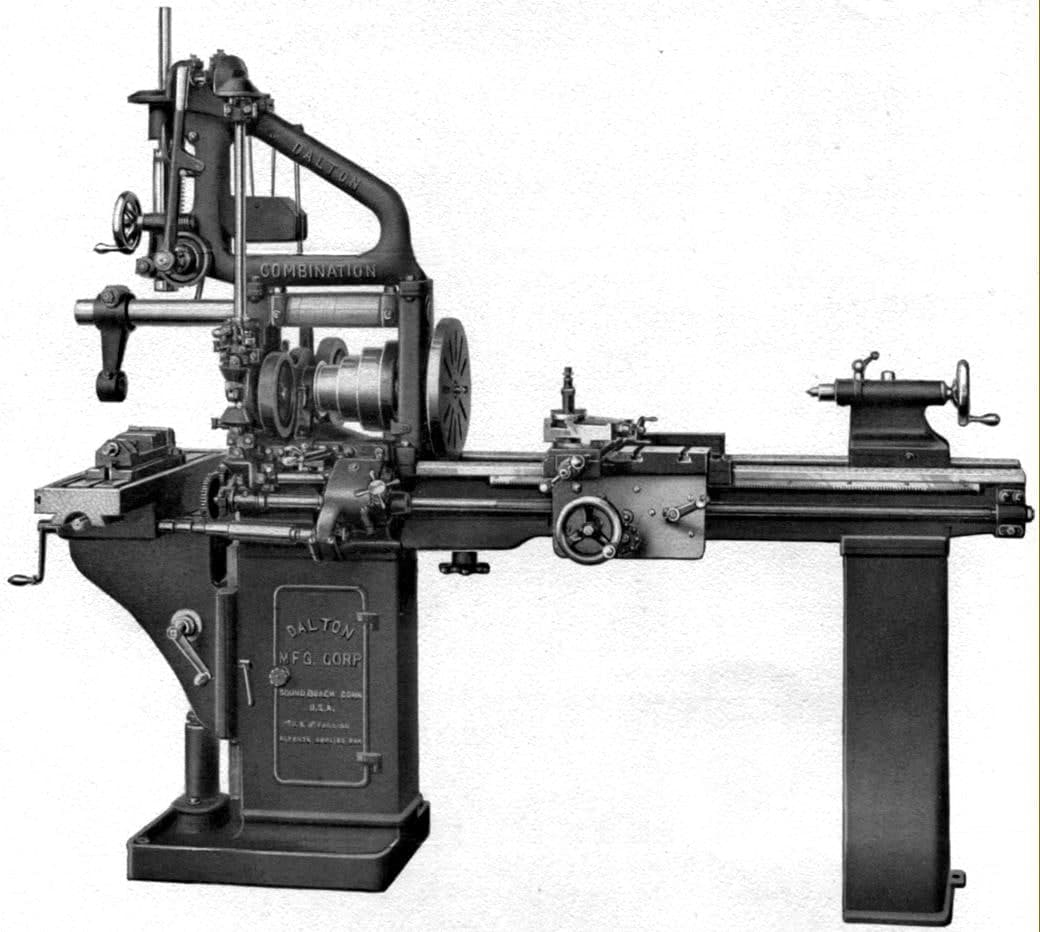
\includegraphics[width=0.7\textwidth]{ch-1/dalton}
	}
	\caption{Dalton Combinantion Machine}\label{fig:dalton}
\end{figure}

\paragraph{Piho Combination Machine}

Piho Combination Machine~(рисунок~\cref{fig:piho}) "--- комбинированный универсальный станок, производимый в конце 1940-х годов компанией Hartensteiner Maschinenfabrik, рекламировался производителем как устройство, которое будет использоваться в ремонтных мастерских. Существовало два типоразмера: б\'ольшая версия имела возможность регулирования высоты заднего центра в диапазоне от 175 до 300\:мм и межцентровое расстояние равное 1300 мм; меньшая (настольная версия) "--- от 60 до 100\:мм и 180\:мм между центрами соответственно. Обе модификации могли работать как токарный станок, а также как горизонтальный и вертикальный фрезерный станок.

Несмотря на компромиссы, заложенные в конструкции, в станке были реализованы составные направляющие скольжения, низкоскоростной узел заднего редуктора, ходовой винт, движущийся под станиной, а также был оснащен барабаном для реверса шпинделя и тонкой подачей с ременным приводом. Очевидно, что в качестве токарного станка он работал так же, как и любой другой обычный токарный станок даже меньшего типоразмера. Однако наличие дополнительного фрезерного модуля, позволяло ему приблизится по своим возможностям к современным обрабатывающим центрам. Более того, фрезерный модуль был оснащен пинолью для быстрой подачей для сверления и имел возможность наклона в плоскости, перпендикулярной оси токарного станка. За счет большого размера расточного стола можно было ещё повысить универсальность станка, используя его в качестве горизонтального фрезерного.

\begin{figure}[ht]
	\centerfloat{
		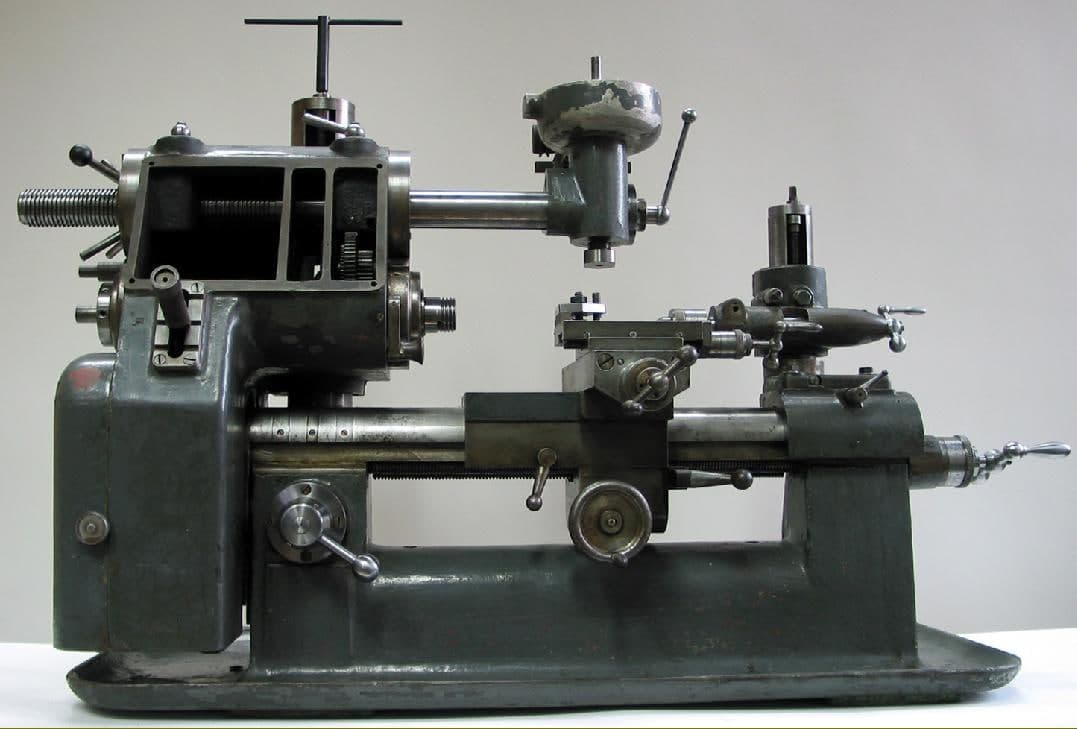
\includegraphics[width=0.7\textwidth]{ch-1/piho}
	}
	\caption{Piho Combination Machine}\label{fig:piho}
\end{figure}

\paragraph{Adcock \& Shipley Combination Machine Tool}

<<Универсал>> Adcock \& Shipley~(рисунок~\cref{fig:adcock-1}) обладал максимальной гибкостью и модульностью по сравнению с другими подобными станками. На площади всего 7 футов на 3 фута для б\'ольшей модели и 11 футов 6 дюймов на 3 фута 8 дюймов для меньшей помещались токарно-винторезный станок, круглошлифовальный станок для внутреннего и внешнего шлифования, вертикальный/горизонтальный фрезерный станок, а также сверлильный станок и специализированные модули для заточки инструмента. Вместо выдвижных или подъемных станин и передней бабки, которые использовались на многих других станках того же типа, Ryder был построен на основе обычного токарного станка, причем каждый отдельный модуль имел автономный привод и мог (кроме шлифовального станка) работать параллельно с другими модулями. Устройство было первоначально разработано для использования на борту корабля и соответствовало различным требованиям, установленным Британским адмиралтейством для этой цели. 

\begin{figure}[ht]
	\centerfloat{
		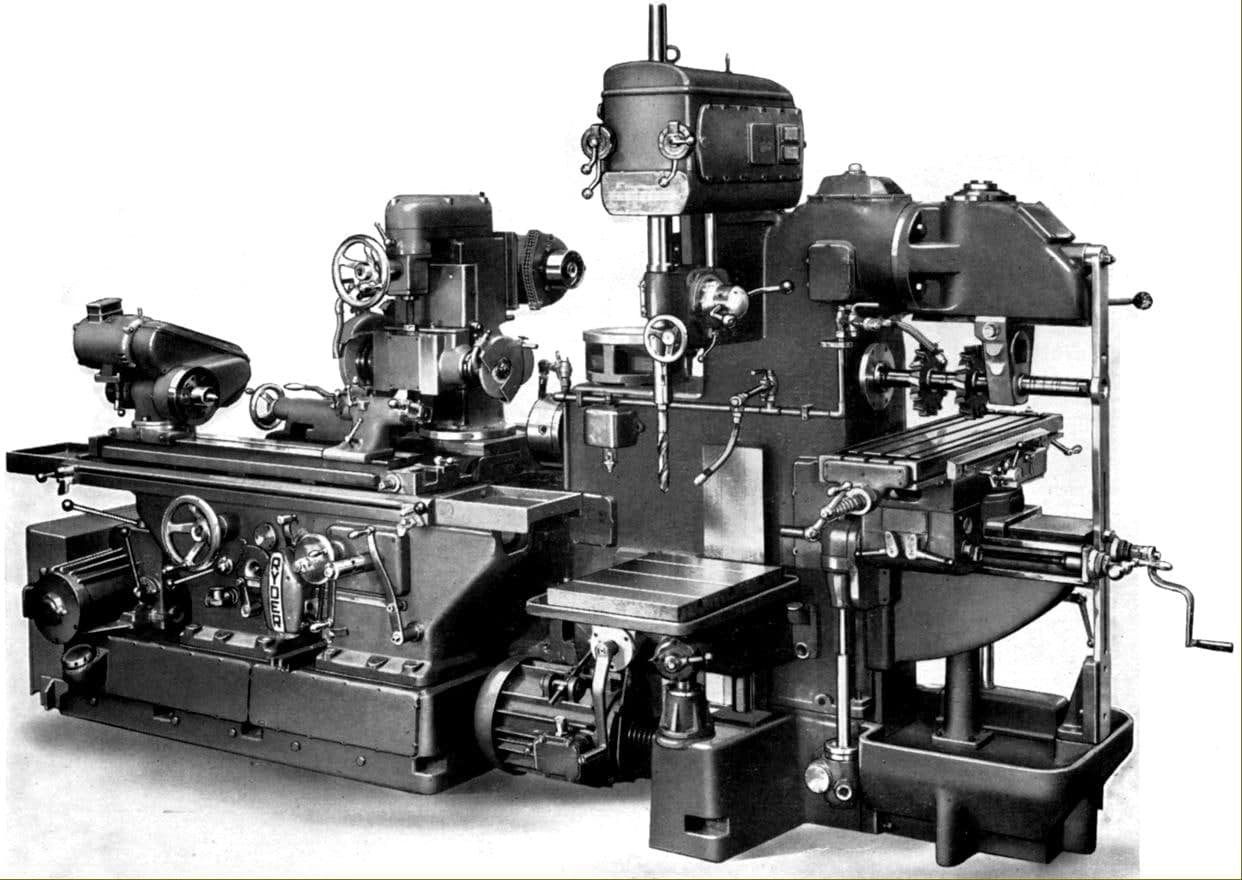
\includegraphics[width=0.7\textwidth]{ch-1/adcock-1}
	}
	\caption{Adcock \& Shipley Combination Machine Toolо, вид спереди}\label{fig:adcock-1}
\end{figure}

Токарный модуль обладал следующими характеристиками: высота над станиной 8 дюймов, расстояние между центрами 18 дюймов, коробка передач из 8 скоростей, обеспечивающая максимальную частоту вращения шпинделя в 1020 об/мин., трехфазный привод на 3 л.с., 1760 об/мин. Проходное отверстие шпинделя было всего 0,75 дюйма, что вряд ли соответствовало той работе, для выполнения которой мог бы потребоваться рассматриваемый станок. Также на станке был установлен упрощенный редуктор для нарезания резьбы с ходовым винтом, позволявшим нарезать дюймовые резьбы с шагом от 4 до 100 ниток на дюйм. Для автоподачи суппорта использовался отдельный ходовой вал, а ходовой винт был нужен исключительно для нарезания резьб.

Фрезерный модуль обладал оригинальной конструкцией с горизонтальным и вертикальным шпинделями. Рабочая поверхность фрезерного стола была размером 26 на 6 дюймов с продольным ходом 10 дюймов и поперечным всего 5,5 дюйма, вертикальный ход стола составлял 10 дюймов, что было крайне мало по сравнению со схожими по размерам универсальными фрезерными станками того времени. Оба шпиндели были рассчитаны на инструмент под конус ISO 40, горизонтальный мог вращаться с частотой от 48 до 970 об/мин, вертикальный "--- от 77 до 1575 об/мин.

Универсальный стол шлифовального станка с возможностью поворота на 45 градусов по часовой стрелке и 15 градусов против часовой стрелки был установлен параллельно станине токарного станка и использовался как опора для шлифовальной головки. Два зубчатых колеса соединяли головку с органами управления в передней части станка. Максимальная высота заготовки над столом составлял 7 дюймов, максимальная длина "--- 10 дюймов. Также была возможна заточка различного режущего инструмента. Подача охлаждающей жидкости к шлифовальной головке представляла собой отдельный блок, разработанный, чтобы избежать загрязнения другой охлаждающей жидкости (подаваемой на токарный, фрезерный и сверлильный модули) абразивными частицами.

Сверлильный модуль устанавливался на задней части <<шпиндельной бабки>> токарного станка и имел шесть скоростей от 420 до 5000 об/мин с мощностью, обеспечиваемой отдельным двигателем мощностью 0,5 л.\,с. Диапазон выбора инструмента был обусловлен использованием в патроне конуса Морзе 1, что ограничивало применение данного модуля для легких работ~(рисунок~\cref{fig:adcock-2}).

\begin{figure}[ht]
	\centerfloat{
		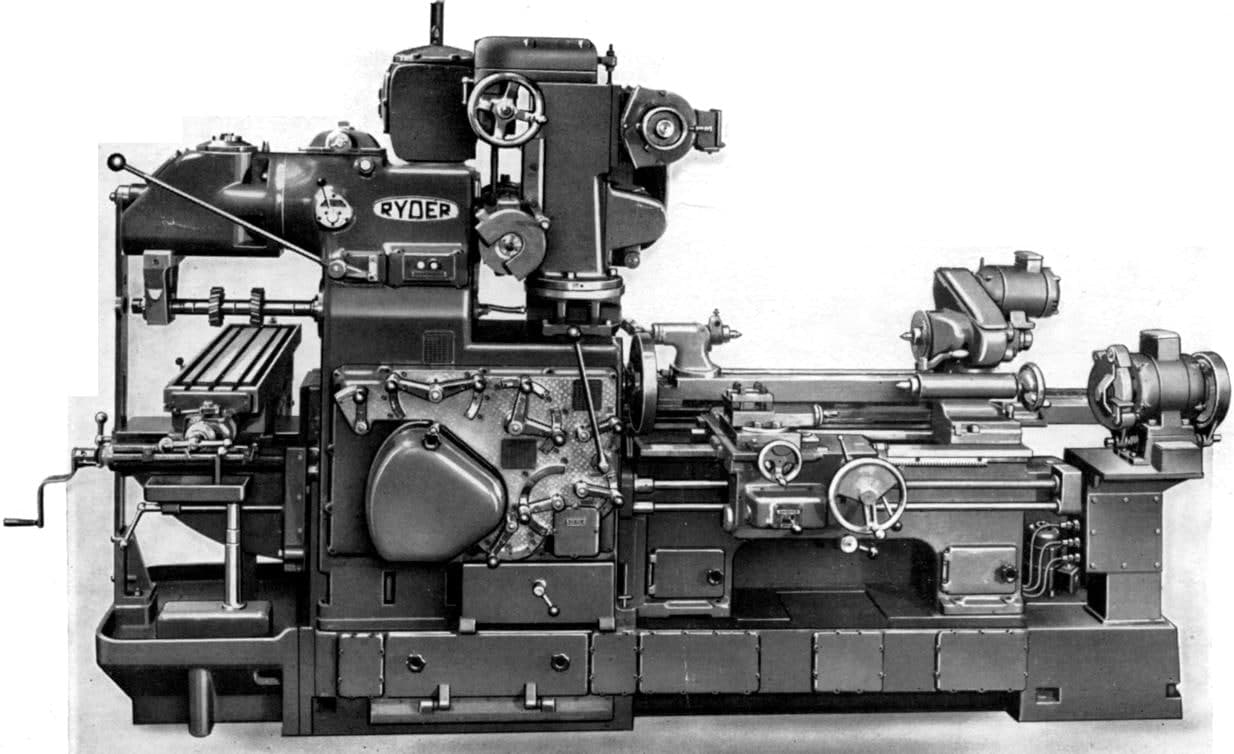
\includegraphics[width=0.7\textwidth]{ch-1/adcock-2}
	}
	\caption{Adcock \& Shipley Combination Machine Tool, вид сзади}\label{fig:adcock-2}
\end{figure}

\subsection{Агрегатные станки}

Агрегатными станками (АС) называется оборудование, которое состоит из стандартизованных и специальных агрегатов, сборочных узлов и деталей~(рисунок~\cref{fig:agr-example}). Доля специально изготовленных узлом при этом меньше доли стандартизованных и нормализованных узлов. Конфигурация агрегатных станков происходит за счёт объединения всех его узлов в единый агрегат (станок, рабочий комплекс). Для данного агрегата всегда используется \textit{общая (монолитная)} системой управления и контроля. АС в подавляющем большинстве случаев применяют в \textit{крупносерийном и массовом производстве}. Первые агрегатные станки управлялись по аналогии со станками-автоматами, повсеместно распространенными в 60--70х годах, затем появились станки с ЧПУ. Это в свою очередь позволило использовать агрегатные станки уже и в серийном производстве. Все современные агрегатные станки управляются с помощью ЧПУ, однако в единичном и малосерийном производстве данный тип оборудования не использовался никогда. На агрегатных станках возможно осуществлять многоинструментную и многопозиционную лезвийную и абразивную механическую обработку деталей. Ранние представители агрегатных станков могли выполнять только один вид обработки (главным образом этим видом обработки было сверление и резьбонарезание). Существующие на текущий момент модели могут комбинировать практически все технологические операции по механической обработке.

\begin{figure}[ht]
	\centerfloat{
		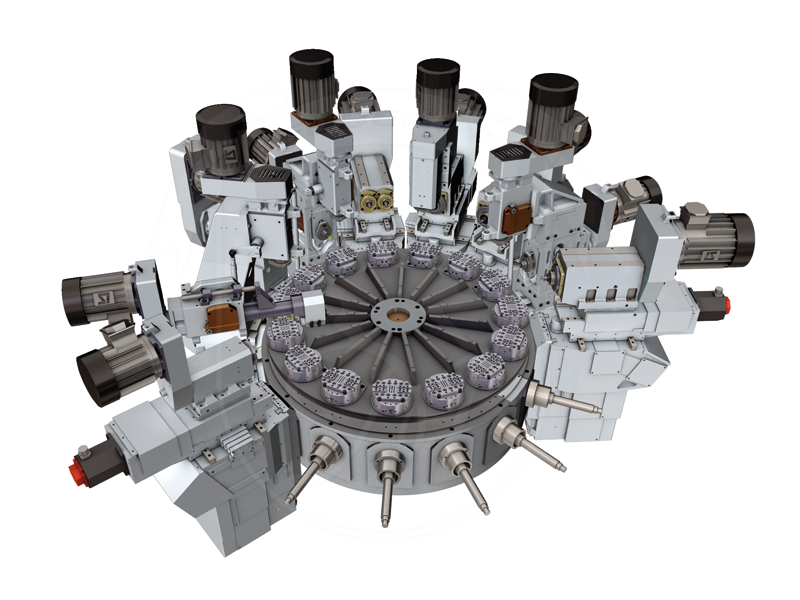
\includegraphics[width=\textwidth]{ch-1/agr-example}
	}
	\caption{Пример агрегатного станка}\label{fig:agr-example}
\end{figure}

Термин <<агрегатный станок>> впервые был использован и применялся в СССР. Однако существовали и существуют зарубежные станочные системы по сути своей являющиеся агрегатными станками. В литературе подобные станки именуются <<реконфигурируемыми производственными системами>>\footnote{От англ. \textit{Reconfigurable Machine Tools}.} или сокращенно RMS~\cite{lee1997reconfigurability, mehrabi2000}. RMS "--- это достаточно широкий класс промышленного оборудования, лишь некоторые разновидности которого соответствуют характеристикам отечественных агрегатных станков.  Так, в патенте~\cite{US6349237} описывается производственная система (станок), имеющая изменяемую структуру. Данная система разработана на основе рыночного спроса и может быть легко изменена для производства различных объёмов продукции одного семейства. Описанная система включает в себя множество рабочих станций с реконфигурируемыми агрегатами, подсистему числового программного управления, включающую множество реконфигурируемых контроллеров, а также реконфигурируемую систему обработки материалов. Также в патенте показано, что предлагаемое аппаратное обеспечение позволяет преобразовывать станки, например, путем перемещения их шпиндельных узлов. Производственные мощности рассматриваемой системы быстро адаптируются к рыночным колебаниям спроса на продукцию. Функциональность легко адаптируется к производству новых продуктов того же семейства. Подобные станки облада.т определенными ключевыми характеристиками (например, модульностью, интегрируемостью, настройкой, конвертируемостью и диагностируемостью), которые необходимы для быстрой и рентабельной реконфигурации. Также в патенте предоставляется методика разработки таких станков и дополнительная методика для изменения производственной мощности, включая реконфигурацию и наращивание парка подобных станков. 

Существуют и другие подобные станочные системы, поэтому в рамках данного обзора под термином <<агрегатный станок>> будут, в частности, подразумеваться и зарубежные системы класса RMS. Как и любое другое оборудование приборостроительного производства, агрегатные станки делятся на специальными и специализированными. Очевидно, что специальные предназначены для обработки одной или несколько деталей одновременно, в свою очередь, специализированные агрегатные станки нацелены на последовательное формообразование нескольких деталей, требующего незначительного изменение конфигурации АС. В зависимости от потребностей производства АС могут работать как автономно, так и в составе гибких производственных систем.

Принцип агрегатирования АС базируется на том положении, что вместо проектирования всех узлов при создании нового станка используют ранее использованные узлы. Из данных узлов получается определенная компоновка, которая и становится новым станком. Для осуществления данного процесса заранее разрабатывается ряд однотипных узлов (агрегатов) разных типоразмеров и мощности приводов (если узел или агрегат включает в себя отдельную силовую часть). Узлы и агрегаты, входящие в этот ряд называются нормализованными или унифицированными. Нормализованные узлы дают возможность спроектировать АС, практически полностью удовлетворяющий используемому технологическому процессу обработки той или иной заготовки. Агрегатные специальные станки обладают рядом существенных преимуществ преимущества перед другими станками, применяемыми в массовом и крупносерийном производстве:

\begin{itemize}
	\item АС позволяют создавать станки специально под конкретный технологический процесс. То есть в случае применения АС у технологов появляется возможность сначала разработать телеологический процесс, а потом сконфигурировать под него АС из уже готовых и отлаженных узлов и агрегатов. При этом нет необходимости оптимизировать или изменять технологический процесс под конкретные производственные возможности.
	\item АС позволяют осуществлять многоинструментную обработку заготовок, что дает возможность существенно повысить производительность производства.
	\item АС дают возможность выполнения разнообразных технологических операций на одном и том же станке путем простое его переналадки.
	\item Использование АС позволяет постоянно и непрерывно улучшать оборудование, используемое на производстве. Появляется возможность модернизироват не весь станок целиком, а лишь тот узел (агрегат), который морально или физически и требует замены.. То же самое касается и ремонтопригодности, сломавшийся узел может быть быстро заменен на такой же работоспособный (находящий в резерве), а после ремонта основного первоначального узла, он будет возвращен на склад хранения, для резерва на случай будущих поломок.
	\item При использовании АС увеличивается надежность\footnote{Здесь под надежностью понимается способность оборудования сохранять в течение продолжительного промежутка времени значения своих основных параметров в заданных интервалах, а также выполнять все свои основные функции при заданных условиях применения. в установленных пределах значения всех параметров, характеризующих способность выполнять требуемые функции в заданных условиях применения.} работы оборудования, созданного из проверенных и отлаженных нормализованных узлов;
	\item В случае необходимости создания специального оборудования, оно также собирается из серийных узлов, что в целом удешевляет его.
\end{itemize}

Тем не менее, помимо плюсов, АС обладают и рядом недостатков, которые в настоящее время сильно сократили спрос на эти станки даже для \textit{массового производства}:

\begin{itemize}
	\item Для каждой новой выпускаемой на производстве детали, даже совсем незначильно отличающейся от уже существующей, необходимо делать (конфигурировать) новый специальный станок.
	\item АС в силу своей универсальности имеют более высокую стоимость, поэтому экономически могут оправдать себя только в условиях реального массового производства.
\end{itemize}

В процессе развития АС были предприняты многочисленные попытки устранения данных недостатков, в частности, было установлено, что специальное станочное оборудование должно удовлетворять трём главным условиям:

\begin{itemize}
	\item позволяло осуществлять быструю переналадку и изменение конфигурации для обработки разных видов деталей при сохранении достаточно высокой производительности полученного в итоге оборудования (это самое главное, потому что стоимость основных средств составляет значительную долю в себестоимости продукции);
	\item позволяло проектировать и изготавливать новые виды оборудования в максимально короткие сроки;
	\item обладало невысокой стоимость, что подразумевает достаточно быструю окупаемость.
\end{itemize}


Стоит отметить, что по большей части АС для \textit{отдельных производственных условий} могут удовлетворять всем этим требованиям. Рассмотрим более подробно принцип унификации, который применяется в АС, в дальнейшем это будет полезно для понимания отличий методики унификации АС и рассматриваемого в данной работе модульного технологического оборудования. Унифицированными (иначе нормализованными) узлами АС называются узлы, конструкции которых проектируются с той целью, чтобы быть основой для любого станка, который будет проектироваться на их основе. Из этого несложно сделать вывод о том, унифицированные узлы могут применяться в станках самых разных конфигураций. К нормализованных узлам АС относятся~(рисунок~\cref{fig:agr-machine}):

\begin{itemize}
	\item боковые станины;
	\item станины;
	\item поворотные делительные столы;
	\item силовые бабки;
	\item отдельно стоящие блоки крепления (cтойки); 
	\item проставочные плиты.
\end{itemize}

\begin{figure}[ht]
	\centerfloat{
		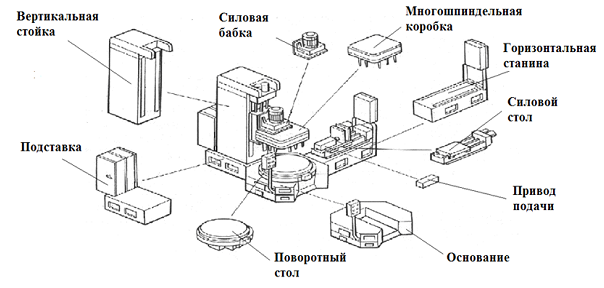
\includegraphics[width=\textwidth]{ch-1/agr-machine}
	}
	\caption{Структура узлов агрегатного станка}\label{fig:agr-machine}
\end{figure}

В случае многошпиндельной обработки большого количества отверстий или при фрезеровании различных плоскостей заготовок корпусных изделий к силовым головкам дополнительно крепятся специальные сверлильные и фрезерные насадки. В случае необходимости создания специальных узлов их компонуют из нормализованных сборок и деталей. Конструкция подобных узлов определяется в соответствии с конструкции детали, которая подлежит обработки на АС. Отечественные реализации АС включали в себя несколько сотен наименований различных унифицированных узлов в более, чем 2500 исполнений и типоразмеров. Из подобных нормализованных агрегатов и сборочных единиц могло состоять до 75--80\% узлов АС.

Необходимо отметить, что основное назначение АС "--- механическая обработка сложнопрофильных изделий. Из этого следует, что общее количество силовых узлов, блоков, включающих в свой состав различные шпиндели, а также само расположение осей шпинделей обуславливается технологическим процессов, выполняемым на АС. Соответственно, по типу АС разделяются на~\footnote{Электронный ресурс: {\tiny\url{extxe.com/3563/agregatnye-stanki/}} (дата обращения: 15.10.2018).}: 

\begin{itemize}
	\item одноагрегатные;
	\item многоагрегатные;
	\item одношпиндельные;
	\item многошпиндельные;
	\item горизонтальные;
	\item вертикальные;
	\item наклонные;
	\item комбинированные;
	\item односторонние;
	\item многосторонние.
\end{itemize}

Очевидно,что однопозиционные АС в первую очередь рассчитаны на один неизменный установ заготовки. При этом обработка происходит с одной стороны, а положение заготовки в процессе обработки не изменяется. На многопозиционных станках, оснащенных поворотно-делительными столами механическая обработка заготовок может осуществляться в параллельном или последовательном режиме, но сразу в нескольких разных позициях относительно обрабатывающих инструментов.

Из всего вышесказанного можно сделать вывод о том, что основными нормализованными узлам АС являются так называемые силовые головки, определяющие технологическую операцию. В современных АС каждая силовая головка снабжена отдельным автономным электроприводом, поэтому могут сообщать какому-либо инструменту главное движение, либо осуществлять перемещение, например, делительного устройства. Для каждой силовой головки предусмотрен свой жестко запрограммированный цикл перемещения, включающий в себя подвод инструмента на ускоренной подаче, непосредственно рабочий ход инструмента (их может быть несколько в зависимости от технологического процесса), при необходимости может быть реализована выдержка в жёстком упоре и отвод инструмента на ускоренной подаче с последующем остановом. Как уже отмечалось ранее, первые образцы АС реализовывали данную циклограмму механически с помощью вращающегося кулачка, современные образцы АС реализуются ее исключительно посредством ЧПУ.

Параметры каждой силовой головки являются основанием для использования ее для конкретной технологической операции. К основным параметрами силовых головок относят:

\begin{itemize}
	\item мощность электропривода, обеспечивающего главное движение;
	\item наибольшее усилие, которое может быть приложено к заготовке при подаче;
	\item частота вращения приводного вала шпинделя обрабатывающей головки;
	\item пределы перемещения при линейной или круговой подаче;
	\item скорость холостого хода при перемещении заготовки относительно инструмента;
	\item скорость рабочего хода при перемещении заготовки относительно инструмента;
	\item длина рабочего хода при линейном перемещении;
	\item габаритные размеры блоков и головок.
\end{itemize}

Необходимо отметить, что силовые головки являются не единственными блоками АС. Для выполнения силовых операций: фрезерования с большим съёмом материала, растачивания, подрезки торцов большого диаметра требуются блоки большей жесткости. Для повышения жесткости силовых головок разработчики данной концепции пришли к следующему решению: в силовой головке разделили агрегаты, обеспечивающие главное движение и движение подачи. Таким образом, получилось два разных независимых узла: силовая бабка для реализации главного движения и отдельный силовой стол для обеспечения движения подачи.  

Помимо блоков, обеспечивающих прямолинейное движение заготовки по отношению к инструменту в АС часто использовались делительно-поворотные столы, основной задачей которых было закрепление специализированных приспособлений с заготовками. Данные столы обеспечивали поворот заготовки по отношению к инструменту на определенный угол. Также имелась возможность перемещать обрабатываемые заготовки из одного рабочего положения (установа) в другое. В этом случае заготовка была опять же была точно зафиксирована относительно режущего инструмента. 

Поворотные столы могли быть в вертикальном или горизонтальном исполнениях. Форма столов чаще всего была либо кольцевая, либо дискообразная. Такие столы перемещались только в горизонтальной плоскости. Если поворотный стол осуществлял вращение в вертикальной плоскости, то такой блок именовался <<барабан>>. При использовании барабанных блоков, приспособления с закрепленными в нем заготовками располагалось на периферийной поверхности барабана и заготовку можно было обрабатывать с двух сторон одновременно.

К современным станкам, которые могут быть отнесены к классу агрегатных, можно отнести Mikron MultiX\footnote{Электронный ресурс: {\small\url{https://www.mikron.com/machining-solutions/machining-systems/highly-productive-systems/multix/}} (дата обращения: 14.07.2018).}~(рисунок~\cref{fig:mikron}). Данное оборудование представляет собой платформу, являющейся основой для установки разнообразных станции обработки. Платформа выступает в качестве базового агрегата, а обрабатывающие станции являются сменными блоками. Существует три типоразмера базового агрегата, различающиеся количеством устанавливаемых на них блоков. Конфигурация платформы подбирается под конкретный технологический процесс.

\begin{figure}[ht]
	\centerfloat{
		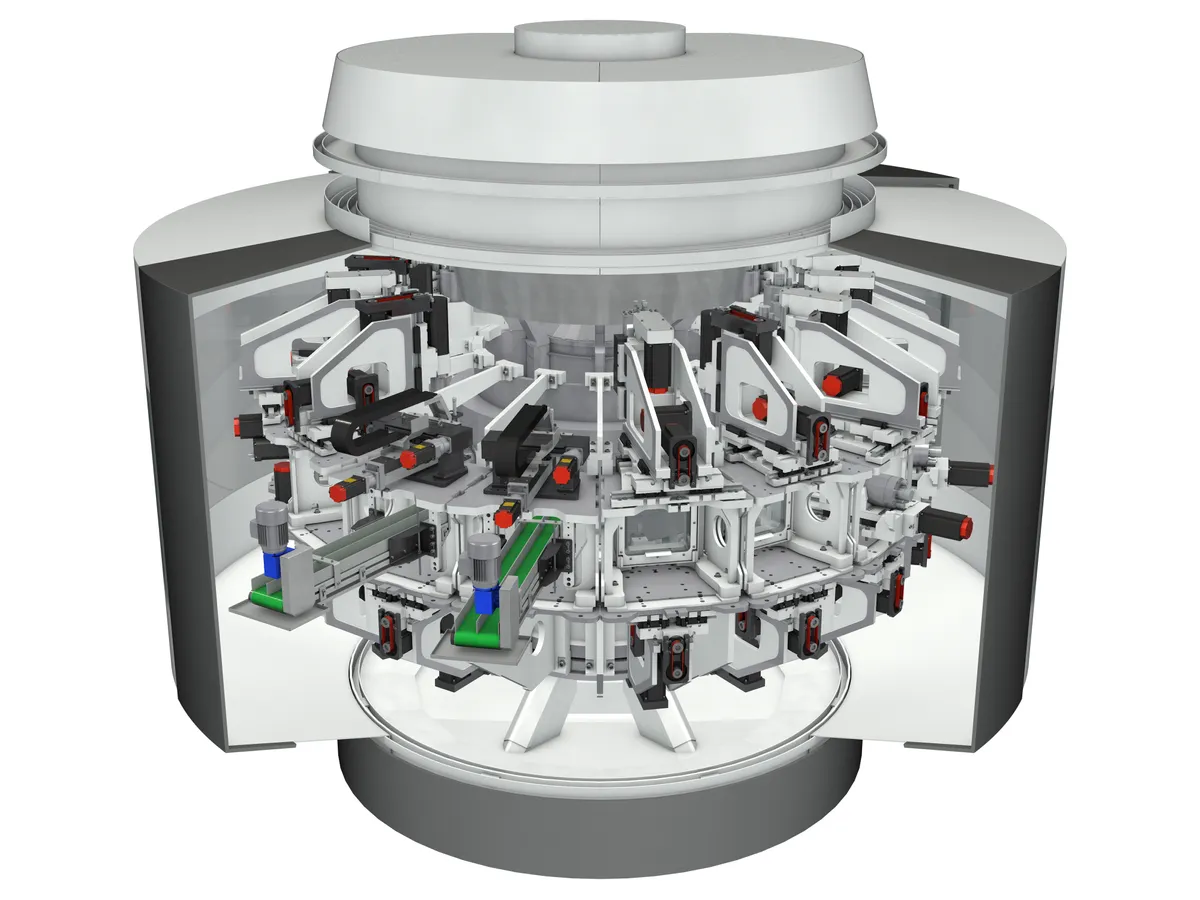
\includegraphics[width=0.7\textwidth]{ch-1/mikron}
	}
	\caption{Агрегатный станок Mikron MultiX}\label{fig:mikron}
\end{figure}

Таким образом, получается, что унификация и стандартизация АС сильно усложняется, т.\,к. конструкция не может быть разделена на равные по своим возможностям и габаритам блоки. По сути АС "--- это сложный унифицированный станок-автомат, где каждый блок имеет несколько разных исполнений, что в общем дает большое разнообразие полученного таким образом оборудования, но это оборудование нельзя считать модульным. Блоки АС неуниверсальны и могут выполнять свои функции только вместе с другими блоками, проектирование которых происходило одновременно. Агрегатные станки унифицированы только по присоединительным размерам и нет центрального блока, на который могли бы устанавливаться другие блоки, изменяя тем самым основную функцию оборудования. Также стоит еще раз повторить, что в основном АС применялись только для металлообработки и никогда не использовались для других видов обработки. На сегодняшний день в силу своей сложности и узкой направленности АС потеряли актуальность даже в рамках массового производства, однако сами базовые подходы, которые были положены в основу их функционирования могут и должны быть использованы для создания универсального модульного оборудования для условий мелкосерийного и единичного производства.

\section{Академические разработки в области модульного технологического оборудования} 

Наиболее полным отечественным исследованием, посвященном теме модульного оборудования является монография Олега Ивановича Аверьянова <<Модульный принцип построения станков с ЧПУ>>~\cite{averianov}. В работе дана комплексная оценка модульного принципа построения многоцелевых станков с ЧПУ, разработанная в московском экспериментальном научно-исследовательском институте металлорежущих станков. Автором проанализированы тенденции развития производства станков, актуальные на период конца 80-х годов, в том числе рассмотрены различные серийные и экспериментальные металлорежущие станки отечественного и зарубежного производства (к сожалению, подавляющее большинство указанно оборудования уже сняты с производства). Также указаны области рационального применения многоцелевых станков с использованием соответствующего математического аппарата. В данной работе теоретически описаны и алгоритмически подтверждены многие гипотезы, связанные с применением модульного оборудования именно в единичном и мелкосерийном производстве.  Однако на момент написания данной монографии основой промышленности были металлорежущие станки, поэтому другие виды обработки в рамках описанной модульной структуры автором не рассматривались. Более того, понятие <<информационные технологии>> в то время ещё не существовало, поэтому система ЧПУ в работе рассматривается как некоторый автомат по перемещению рабочих органов в пространстве (по аналогии со станками-автоматами механически управляемыми посредством кулачков). Естественно, возможность создания модульной децентрализованной автоконфигурируемой системы ЧПУ даже не рассматривается. В связи с распадом Советского Союза и отказом от плановой экономики, наработки, представленные в работе О.\,И Аверьянова. перестали быть актуальными, однако сама методическая основа построения модульного технологического оборудования могут и должны получить развитие в новых современных модульных системах.

Помимо О.\,И.~Аверьянова вопросами разработки модульного оборудования занимались такие отечественные исследователи, как В.\,Н.~Бетин~\cite{betin}, Л.\,П.~Бобрик~\cite{bobrik}, Л.\,С.~Брон~\cite{bron}, Д.\,А.~Куприянов~\cite{kuprianov}, В.~В.~Вяткина~\cite{minhat2009stepncmilluoa} и другие. 
	
Также существует достаточное количество зарубежных исследований, посвященных данной теме. Предпосылками к исследованиям в данной области стали многофункциональные универсальные металлорежущие станки, которые были описаны в разделе~\cref{sec:ch1/multifunc-machines}. Данное оборудование реализовывалось для решения конкретных технологических задач, при этом изначально какие-либо исследования самого принципа модульности не проводились. Модульная конструкция станка претерпевала постепенные изменения, модернизировалась и развивалась в различной степени с 1930-х годов. При этом менялась конструкция базового агрегата, система строительных блоков, применялся модульный дизайн, холонический дизайн, принципы реконфигурируемости конструкции и т.\,д. Концепция и метод модульного проектирования для структурной конфигурации приписываются Г.~Шлезингеру и Ф.~Кенигсбергеру. Первый предложил концепцию на примере конструкции передней бабки радиально-сверлильного станка, а второй применил этот метод к конструкции фрезерного станка марки Wanderer~[Spur, G., Produktionstechnik in Wandel, Carl Hanser Verlag, M{\"u}nchen/Wien, 1979]. Изначально термин <<модуль>> авторами не использовался, вместо этого подобный подход называли <<системой строительных блоков>>. Этот термин окончательно был заменен термином <<модульная конструкция>> самим профессором Кенигсбергером примерно в 1967\,г.

С этого момента и до сегодняшнего дня модульная конструкция в различной степени охватывала такие сферы зарубежных исследований, как проетирование производственных систем и станков, программного обеспечения и режущего инструмента. Сейчас происходит продвижение модульного принципа в некоторые новые области исследований промышленного производства. Например, в монографии Йошими Ито~\cite{ito2008modular} рассматривается модульный принцип конструирования металлорежущего оборудования с числовым программным управлением, представлены методы, позволяющие сократить время проектирования подобных модульных систем, повысить надежность их функционирования, снизить эксплуатационные затраты и упростить обслуживание и ремонт. В работе рассмотрены основы модульного проектирования технологического оборудования, методика определения характеристик модульных станков, описаны примеры применение модульных станков. Также рассматриваются принципы взаимодействия модулей в информационном плане и методика тестирования модульного оборудования.

Среди прочих работ можно выделить работу Светика~\cite{svetlik2020modularity}, посвященную модульному принципу построения производственных систем, в частности модульного технологического оборудования. Предложена концепция модульной технологической системы, разработана математическая модуль функционирования и сборки подобных систем, определены основные их параметры. Рассмотрены примеры предложенной концепции в приложении к различным видам технологического оборудования: промышленным роботам, обрабатывающим центрам и логистическим системам.

В работах Бортолини~\cite{bortolini2019reconfigurability, bortolini2019dynamic} приведен пример применения модульного подхода в ячеистом производстве~(сокр.~\textit{ЯП}). Показано, что обычно в ЯП каждая ячейка используется для определенного семейства деталей, что сокращает объём использованного материала, время погрузочно-разгрузочных операций, а также объём незавершенного производства. Предлагается модифицировать имеющееся ЯП посредством внедрения модульного подхода. Автором предложена оригинальная модель оптимизации, основанная на теории линейного программирования, для разработки альтернативной маршрутизации деталей. В данной модели ЯП строиться из реконфигурируемого оборудования, состоящего из множества основных и вспомогательных модулей. При использовании различных вспомогательных модулей на одной и той же единице реконфигурируемого оборудования становятся доступными различные операции. В предлагаемом подходе происходит оптимизация набора модулей и маршрутизация движения объектов производства между ячеками ЯП. Проведен сравнительный анализ, в которой сопоставляется предложенная и традиционная модели ЯП. Анализ показывает, что предложенная модель позволяет уменьшить время на перемещение объектов производства между ячейками на 58,6\%, а общее снижение времени примерно на 53,3\%.

Ли в работе~\cite{li2020modular} была описана информационная модель модульного проектирования станков с ЧПУ на основе  потребительского спроса, путём анализа требований клиентов. На основе предложенной функции качества получается базовая структура станков, а в результате анализа нечеткой кластеризации получается уточненное функциональное разделение на модули и формируется диаграмма динамической кластеризации. На основе метода предпочтения порядка по подобию оценивается окончательная схема разделения модулей станков. Предложенная методика разделения на модули проверяются на примере горизонтально-фрезерных станков с ЧПУ компании Shenyang Machine Tool Group. Анализ полученной в результате конструкциии доказывает, что система модульного разделения является эффективной для данного типа оборудования. Похожая методика описана в работе Шень~\cite{sheng2017lifecycle},только в качестве метрики оценки эффективности получаемой модульной конструкции здесь используются параметры жизненного цикла изделия.  

\section{Модульные системы управления технологическим оборудованием}\label{sec:ch1/sec2}
%Добавить сюда про смузи и LinuxCNC

Анализируя эволюцию современной индустрии, можно сделать вывод о том, что наиболее многообещающим направлением развития является создание гибких распределенных автоматизированных производственных линий. Новая концепция массового производства была создана в результате Четвертой промышленной революции (или Индустрии 4.0) и постепенного распространения индустриальных кибер-физических систем. Подходы, применяющие жесткую последовательную логику реализации этапов технологического процесса в крупносерийном и массовом производстве постепенно преобразуются для условий мелкосерийного производства на заказ. Как уже отмечалось ранее, продолжается развитие малых инновационных предприятий. В итоге меняется подход к проектированию современного интеллектуального оборудования.

Первые станки с числовым программным управлением появились в середине XX~века. Основной областью применения такого оборудования изначально было массовое производство. Первые системы числового программного управления были сложными и дорогими. Для внедрения таких систем в существующее производство требовался длительный период пуско-налодочных работ и обкатки на конкретном технологическом процессе. Станки с ЧПУ крайне плохо поддаются модернизации, поэтому период их эксплуатации является достаточно длительным и может достигать нескольких десятилетий.

Данные обстоятельства сильно мешают при внедрении современных информационный технологий в промышленность. Это обуславливается тем, что даже незначительное изменение структуры производства требует полного изменения производственного цикла, либо, как минимум, создания вспомогательных уровней управления на уровне цехов и участков.В противном случае невозможно грамотно интегрировать старое оборудование с современной кибер-физической системой. Однако данный этап неизбежен при постепенном смене парка технологического оборудования и перехода к новым подходам в производстве.
Следовательно, необходимо переосмыслить саму парадигму проектирования оборудования с ЧПУ, и возможность подключения нового оборудования к информационной среде связи по открытому протоколу становится весьма важной.

Современными исследователями были предприняты попытки реализации подобного подхода. Например, Григорьев и Мартынов в своих исследованиях предлагают подход к разработке гибкого ядра ЧПУ на основе программной платформы, реализованной в виде автономных библиотечных модулей. Открытая архитектура этой системы включает в себя различные абстрактные уровни, относящиеся к различным человеко-машинным интерфейсам, и возможность описания компонентов системы на разных языках программирования. Подключение компонентов системы осуществляется через шину Fieldbus~\cite{Grigoriev2014517}.

Бин и др. описывают открытую платформу для создания систем ЧПУ, эта система состоит из набора многоцелевых компонентов, которые могут использоваться многократно, и набора коммуникационных модулей для их соединения~\cite {Bin200473}. Похожий подход представлен в статье Ма~\cite{MA2007272}.
Моралес-Веласкес и др. предложена система (платформа) ЧПУ с открытой архитектурой на основе многоагентной системы программных и аппаратных компонентов под названием MADCON. Аппаратные блоки предлагаемой ими системы объединяют функции управления и мониторинга, обеспечивая открытую архитектуру на основе ПЛИС для реконфигурируемых приложений. Программные компоненты используют структуру XML для файлов описания системы, объединяя такие функции, как язык описания блок-схем и графический пользовательский интерфейс~\cite{MoralesVelazquez2010407}.

Работы Вербы~\cite{Verba2016} и Празереса~\cite{Prazeres7471301} посвящены концепции <<Туман вещей>>\footnote{Сокр. от англ. \textit{Fog of Things}}. Эта концепция представляет собой современную интерпретацию Интернета вещей\footnote{От англ. \textit{Internet of Things}.}, который, по сути, является основой многих индустриальных кибер-физических систем. Туман вещей позволяет создать более однородную информационную среду связи, тем самым улучшая и упрощая протокол связи компонентов.

В работе Хана~\cite{han2007development} рассматривается контроллер с открытой архитектурой, который может быть основой для различного оборудования с ЧПУ. Разрабатываемый контроллер имеет модульную архитектуру, а в качестве аппаратной  платформы использует персональный компьютер. Основная цель работы "--- разработать методику построения программно-аппаратная платформа системы ЧПУ. Также исследуются методы статического моделирования контроллера с открытой архитектурой, включающие технологию объектно-ориентированного программирования, технологию применения динамических библиотеки и разделения  системных модулей. Авторы обсуждают динамическое моделирование поведения  и представление потока данных контроллера с открытой архитектурой, которые  описаны с помощью иерархической модели конечного автомата. Для разработки  библиотеки программных функциональных компонентов авторы создали модель  многократно используемого программного модуля. В качестве испытательного  стенд выступает трёхосевой фрезерный станок. Для данного станка был успешно  разработан программный код системы ЧПУ, основанной на описанной библиотеке функциональных модулей с применением методики конфигурирования  системы. Результаты экспериментов показывали, что, помимо увеличения степени повторного использования программного кода и открытости, применение  вышеупомянутой методологии приводит к значительному сокращению времени  разработки, а также стоимости обслуживания конечного оборудования с ЧПУ.

\section{Промышленные аналоги предлагаемой модульной платформы}\label{sec:ch1/industrial-examples}
%Добавить сюда из материалов


В настоящем разделе будут рассмотрены проекты и готовые продукты, которые обладают свойством модульности и возможности переналадки. Первый критерий по, которому проходило сравнение "--- \textit{универсальности рабочего органа}, то есть возможность путём простой переналадки менять тип оборудования. 

На сегодняшний день на рынке представлены несколько типов универсальных модульных настольных станков нижнего ценового диапазона. Одним из наиболее известных производителей подобного оборудования является компания \textit{Proxxon}~(рисунок~\cref{fig:proxxon}), выпускающая различные настольные станки <<хоббийного>> класса, в основном токарно-фрезерно-сверлильной группы, распиловочное оборудование и ручной электроинструмент. Большое количество универсальной оснастки и~взаимозаменяемость многих частей оборудования Proxxon позволяет использовать его в небольших мастерских, а также на малых инновационных предприятиях, но с рядом ограничений:

\begin{itemize}
	\item В базовой комплектации все оборудование ручное. Возможность переделки под числовое программное управление является опцией. Возможности ЧПУ сильно ограничены.
	\item Спецификации оборудования закрыты, создание своих модулей невозможно, либо возможно, но только с~применением реверс-инжиниринга.
	\item Все оборудование Proxxon субстрактивного типа, возможность использовать его для создания 3d-принтера или контрольно-измерительной машины отсутствуют, так как нет единой модульной структуры блока управления ЧПУ, а также фирменного программного обеспечения.	
\end{itemize}

\begin{figure}[ht]
	\centerfloat{
		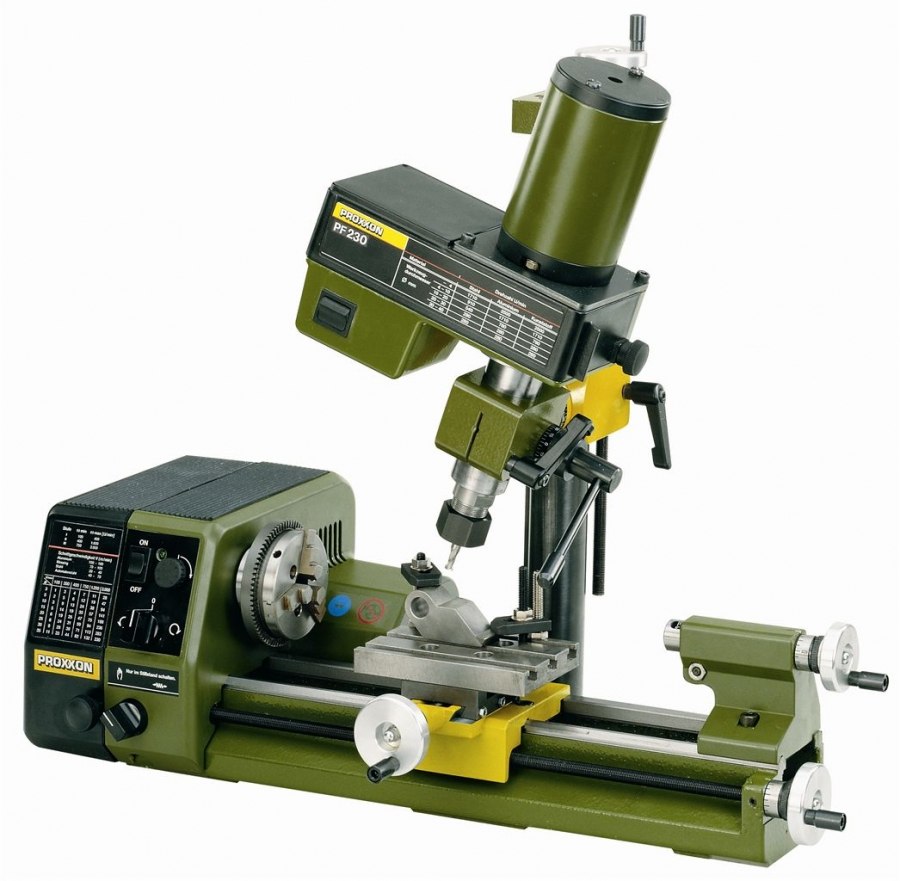
\includegraphics[scale=0.27]{ch-2/image1.png}
	}
	\caption{Пример оборудования компании Proxxon}\label{fig:proxxon}
\end{figure}

Стоит также отметить настольные модульные универсальные станки, выпускаемый немецкой компанией TheCoolTool\footnote{Электронный ресурс: {\small\url{thecooltool.com}} (дата обращения: 07.05.2020).}, в~особенности модели UNIMAT~1~(рисунок~\cref{fig:unimat-2}) и UNIMAT CNC~(рисунок~\cref{fig:unimat-2}).

\begin{figure}[ht]
	\centerfloat{
		\hfill
		\subcaptionbox{\label{fig:unimat-1}}{%
			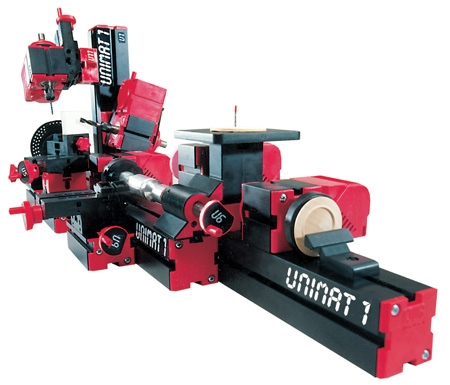
\includegraphics[width=0.4\linewidth]{ch-2/image2}}
		\hfill
		\subcaptionbox{\label{fig:unimat-2}}{%
			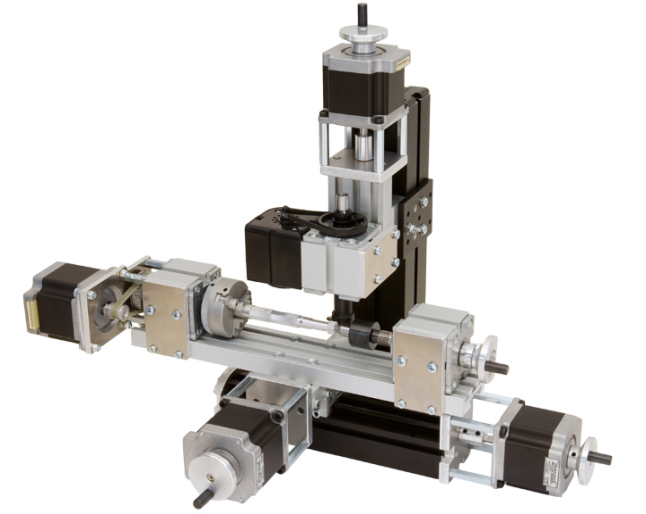
\includegraphics[width=0.4\linewidth]{ch-2/image3}}
		\hfill
	}
	\caption[Настольные модульные станки UNIMAT 1 и UNIMAT CNC]{Настольные модульные станки UNIMAT 1 (\textit{а}) и UNIMAT CNC (б)}\label{fig:unimat}
\end{figure}

Первый из рассматриваемых станков представляет собой модульную систему <<6 в 1>> с ручным управлением (переделка под ЧПУ возможна только с применением специальных доработок и реверс-инжиниринга), то есть позволяет в зависимости от компоновки модулей производить:

\begin{itemize}
	\item Распиловку деревянных и металлических заготовок вертикально расположенным ножовочным полотном.
	\item Токарную обработку деревянных заготовок.
	\item Токарную обработку металлических заготовок.
	\item Плоское торцевое шлифование с возможностью снятия шлифовального блока для ручной обработки шлифовальным кругом.
	\item Вертикальное и горизонтальное фрезерование.
	\item Сверление с возможностью поворота сверлильной головки на 360$^{\circ}$ или снятия её для ручного сверления.
\end{itemize}

Возможность совмещения двух операций без переналадки оборудования отсутствует.

Второй является токарно-фрезерно-сверлильным модульным станком с ЧПУ, в котором в зависимости от компоновки существует возможность управления шестью осями одновременно, что позволяет совмещать операции обработки без перенастройки модулей. Достоинством данного оборудования является большая открытость программной архитектуры, что подтверждается возможностью использовать для управления осями станка не только фирменное закрытое программное обеспечения, но и открытое решение EMC2, построенное на базе свободной операционной системы Linux. При этом сам станок представляет собой лишь набор управляемых электроприводов без внутреннего блока управления, что требует постоянного подключения к персональному компьютеру, приобретаемому отдельно.

К недостаткам можно отнести:

\begin{itemize}
	\item закрытую аппаратную архитектуру рассматриваемого продукта, что существенно усложнит переделку данного решение подо что-то отличное от металлообрабатывающих станков;
	\item неудачную геометрическую компоновку станка, что также ставит по сомнение возможность его переделки под другие нужды (например, очевидно, что подобная кинематическая схема вряд ли позволит использовать ее в качестве трёхмерного принтера или контрольно-измерительной машины);
	\item отсутствие портала, что влечет за собой снижение жёсткости связки координатных осей, а, следовательно, и жёсткости станка в целом. Последнее будет особенно заметно при максимально удалении осей, из-за чего может пострадать точность обработки. Данное предположение подтверждается спецификациями, размещенными на сайте производителя, где указывается, что точность установки не может превысить 80\,мкм.
	\item низкую мощность приводов осей, а также очень небольшие рабочие ходы по некоторым из них.
\end{itemize}

Получается, что за исключением возможности использования свободного программного обеспечения рассматриваемый продукт не является модульном в полном смысле этого слова, это переналаживаемый станок с расширенными возможностями ЧПУ.

Второй параметр, по которому проводилось сравнение с существующими аналогами "--- \textit{открытая аппаратная архитектура}, позволяющая создавать новые типы оборудования без необходимости создания каких-то дополнительных переходных блоков и применения реверс-инжиниринга.

Для сравнения были рассмотрены два проекта, целью которых является создание открытой платформы универсального оборудования с ЧПУ:

\begin{enumerate}
	\item Build Your Own CNC.\footnote{Электронный ресурс: {\small\url{buildyourcnc.com/cnckit2.aspx}} (дата обращения: 31.12.2019).}
	\item Shapeoko.\footnote{Электронный ресурс: {\small\url{shapeoko.com}} (дата обращения: 31.12.2019).}
\end{enumerate}

Рассмотрим оба этих проекта более подробно. \textit{Build Your Own CNC}~(рисунок~\cref{fig:byocnc}) "--- коммерческий проект по созданию универсального сборного оборудования с числовым программным управлением. Может считаться условно открытым, так как с одной стороны на сайте производителя отсутствуют чертежи и прочая техническая документация, необходимая для самостоятельного изготовления того или модуля оборудования (за исключением файлов раскроя основных корпусных деталей), но с другой стороны компания принимает запросы от пользователей на создание новых модулей (новых типов оборудования). Финансирование данных исследований проводится за счёт средств, полученных в качестве пожертвований от пользователей, а также за счёт основного бизнеса компании "--- производства и продажи модулей и готовых сборных устройств.

На сегодняшний день в рамках проекта \textit{Build Your Own CNC} реализовано достаточно большое количество модулей и готовых устройств, среди которых можно выделить:

\begin{itemize}
	\item Установку для лазерной резки и гравирования.
	\item Трёхкоординатное фрезерные и сверлильные станки различных компоновок и типоразмеров со множеством сменных головок, среди которых необходимо выделить печатающую головку, позволяющую создать на основе предлагаемой платформы 3d-принтер типа FDM\footnote{Сокр.~от~англ. \textit{Fused Deposition Modeling} "--- моделирование методом наплавления.}.
	\item Распиловочные вертикальные станки.
	\item Установку для автоматического размещения электронных компонентов на печатной плате\footnote{Англ. \textit{Pick and Place machine}.}
\end{itemize}

\begin{figure}[ht]
	\centerfloat{
		\hfill
		\subcaptionbox{\label{fig:byocnc-1}}{%
			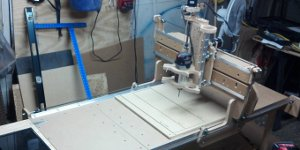
\includegraphics[width=0.5\linewidth]{ch-2/image4}}
		\hfill
		\subcaptionbox{\label{fig:byocnc-2}}{%
			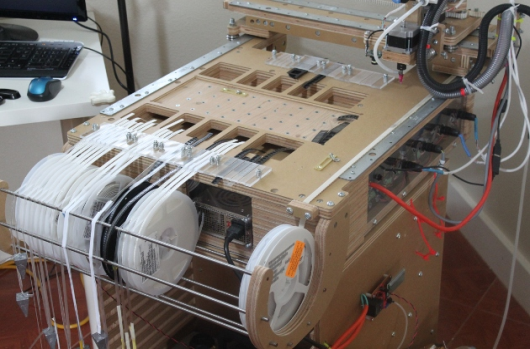
\includegraphics[width=0.5\linewidth]{ch-2/image5}}
		\hfill
	}
	\caption[Примеры оборудования, созданного в рамках проекта \textit{Build Your Own CNC}]%
	{Примеры оборудования, созданного в рамках проекта \textit{Build Your Own CNC}: фрезерный станок портального типа (\textit{а}), установка для позиционирования электронных компонентов на печатной плате (\textit{б})}\label{fig:byocnc}
\end{figure}

В планах компании также разработать:

\begin{itemize}
	\item Пятикоординатный фрезерный станок.	
	\item 3d-принтер, использующий технологию фотолитографии.
	\item 3d-принтер, использующий технологию селективного лазерного спекания.
	\item Станки токарной группы.
	\item 3d-сканер.
\end{itemize}

К недостаткам данного проекта можно отнести следующие:

\begin{itemize}
	\item Как уже отмечалось ранее, проект не является полностью открытым с точки зрения аппаратного обеспечения.
	\item На текущий момент реализовано очень малое количество типов оборудования. Отчасти это связано с первым недостатком, так как спецификации закрыты и разработкой новых модулей и типов оборудования занимаются только сотрудники компании.
	\item Отсутствует единая универсальная кинематическая схема, из-за чего для каждого нового вида оборудования необходимо проектирование новой кинематической схемы, а также сопутствующие этому процессу расчеты и моделирование.
	\item Отсутствует единый подход к проектированию линейных приводов. Предполагается возможность использования как ходовых винтов с трапециевидной резьбой, так и передач на основе зубчатых ремней и цепей. Особо настораживает использование цепных передач в прецизионных настольных станках для установки электронных компонентов на плату.
	\item Основной материал, из которого изготавливаются все несущие и корпусные детали всех видов оборудования "--- клеевая фанера. При всех очевидных достоинствах данного материала таких, как легкость обработки, хорошее виброгашение, высокая прочность, низкая цена, целесообразность использования данного материала для создания высокоточного оборудования с ЧПУ вызывает большие сомнения. Очевидно, что авторам проекта вряд ли удалось достичь высокой жесткости конструкции и точность оборудования оставляет желать лучшего.
	\item Привода всех модулей и всех типов готового оборудования не имеют никаких датчиков обратной связи по положению. Авторы проекта исходят из предположения, что используемые ими шаговые двигатели никогда не пропускаю шагов, драйверы шаговых двигателей всегда генерируют правильную последовательность импульсов, а используемые кинематические схемы не подвержены заклиниванию.
	\item Компания не занимается производством или разработкой блоков управления для своего оборудования и вообще каких-либо электронных или электрических компонентов. Клиентам предлагаются готовые силовые блоки сторонних фирм, а~управление отдается либо на откуп персонального компьютера, либо известной платформе разработки и отладки электроники Arduino.
	\item Также компания не занимается разработкой программного обеспечения для своего оборудования. Пользователям предлагается воспользоваться либо уже упоминавшимся ранее открытым пакетом EMC2, либо приобрести одно из многочисленных коммерческих решений с тем же функционалом.
	\item Даже в проектах отсутствует какое-либо упоминание блока автоматической смены инструмента.
\end{itemize}

Второй проект, выбранный для обзора "--- \textit{Shapeoko}~(рисунок~\cref{fig:shapeoko})"--- является полностью открытым проектом по созданию трёхкоординатной платформы портального типа. Из очевидных достоинств проекта можно выделить созданное авторами проекта программное обеспечение с открытым исходным кодом, а также полностью открытые спецификации аппаратной части, включающие в себя чертежи, трехмерные модели и прочую техническую документацию, необходимую для самостоятельной реализации разработанного авторами оборудования.

\begin{figure}[ht]
	\centerfloat{
		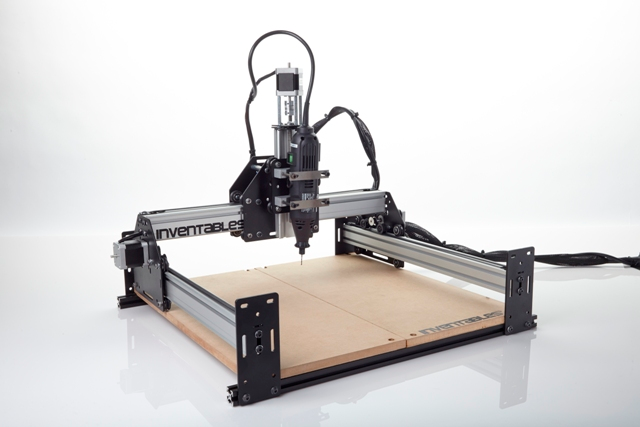
\includegraphics[scale=0.5]{ch-2/image6.png}
	}
	\caption{Трёхкоординатный фрезерный станок, реализованный в рамках открытого проекта \textit{Shapeoko}}\label{fig:shapeoko}
\end{figure}

На данный момент проект находится на очень ранней стадии развития, поэтому не удалось провести детальный и всесторонний анализ недостатков представляемого проекта. Тем не менее, некоторые из них можно выделить уже сейчас:

\begin{itemize}
	\item Проект ориентирован в основном на трёхкоординатную фрезерную обработку и не позиционируется как модульная универсальная платформа.
	\item Управление опять отдаётся на откуп обычного персонального компьютера, за тем лишь исключением, что вместе пакета EMC2 (LinuxCNC) авторы предлагают собственное программное обеспечение. О создании какой-либо модульной электронной системы управления речи не идёт.
	\item Также как и в предыдущем проекте отсутствует какая-либо обратная связь по положению рабочего органа.
	\item Для передвижения портала использованы два шаговых двигателя, никак механически не синхронизированные между собой.
	\item Перемещение портала осуществляется за счёт зубчатых ремней, при этом не предусмотрены датчики обрыва ремня.
	\item Линейное перемещение всех координатных осей осуществляется за счет роликовых кареток. Сложность и~большое количество подвижных частей подобного механизма снижает надежность платформы. Также очевидно, что подобное решение может приводить к заклиниванию осей.
	\item В качестве основного и единственного на сегодняшний день рабочего органа используется гравер.
\end{itemize}

Последний параметр, выбранный для сравнения "--- \textit{модульная открытая архитектура блока управления} в совокупности с открытым исходным микрокодом электронного оборудования.

По данному параметру был найден единственный проект "--- анонсированный на 2015 год корпорацией Google модульный смартфон Ara. Безусловно, трудно производить сравнение модульной системы управления оборудования с ЧПУ и мобильную платформу для создания телефонов и планшетов, но такая цель и не ставилась.

Выбор был обусловлен уникальностью данного проекта. Подобные идеи звучали из уст представителей многих известных компаний и научных центров и ранее, но первая успешная попытка создать достаточно сложное электронное устройство из отдельных взаимозаменяемых модулей была сделана только в этом проекте. Очевидно, что это актуальное направление в ближайшее время получит свое развитие, также очевидно, что оно является очень перспективным и требует всестороннего исследования.

В силу своей специфики достоинства и недостатки проекта Ara рассматриваться не будут, вместо этого будет сделан обзор наиболее интересных и концептуальных решений, реализуемых в рамках данного проекта.

На официальном портале проекта корпорация Google заявляет, что разработала так называемый <<телефон-конструктор>>. Данный конструктор состоит из двух частей: эндоскелета (также часто называемого <<рамой>> и являющегося, по сути, внутренним каркасом) и~набора сменных модулей.

К эндоскелету могут быть подключены процессор со всей необходимой электрической <<обвязкой>>, жидкокристаллический дисплей, дополнительные модули оперативной памяти, физическая клавиатура, камера или дополнительный аккумулятор. Владелец телефон сможет сам производить модернизацию своего устройства или заменять поврежденные модули. Какие-то специальные инструменты или наличие каких-то знаний в области микроэлектроники или программирования не требуются.

Также за счет унификации габаритов эндоскелета и проектируемых модулей можно изменять размер аппарата, предполагается возможность создания как небольшого и очень компактного устройства, так и устройства, сравнимого по своим размерам с современными смартфонами и даже устройства больше похожего на интернет-планшет, а не мобильный телефон.

Очевидное достоинство подобного подхода для пользователя "--- возможность подбирать модули в соответствии со своими потребностями и финансовыми возможностями. Специалисты компании Google говорят, что в минимальной комплектации модульный смартфон будет стоить порядка 50 долларов США, а в максимальной "--- до 500.

Платформа позиционируется как открытая, то есть любой сторонний разработчик, использую так называемый MDK\footnote{сокр.~от~англ. \textit{Module Developers Kit} "--- набор инструментальных средств разработчика для создания модулей.}, сможет выпустить свой модуль, совместимый с Ara.

В спецификации говорится, что некоторые модули могут поддерживать так называемую <<горячую замену>>, то есть возможность сменить модуль без отключения питания аппарата. Также оговорен унифицированный способ крепления модулей к эндоскелету "--- крепление будет осуществляться за счет постоянных магнитов.

Каждый модуль может сочетать в себе несколько различных функций, например, можно создать гибридный модуль, являющийся экраном мобильного телефона и дополнительным аккумулятором, компенсирующим затраты энергии на подсветку и отображение информации.

К сожалению, по состоянию на 2021 год проект Ara в первоначальном состоянии перестал существовать, однако многие наработки, предложенные корпорацией Google, хоть и в несколько упрощенном виде были реализованы в модульном смартфоне Fairphone 3\footnote{Электронный ресурс: {\small\url{fairphone.com}} (дата обращения: 12.12.2019).}.

\section{Современные тенденции в области стандартизации и унификации модульного оборудования}

\subsection{Стандарт МЭК 61499}

Проектирование распределенных систем автоматизации усложняется тем, что не существует единого языка программирования, на котором разработчик мог бы описать всю систему, включая логику каждого узла управления и их взаимодействия. Узлы управления обычно реализуются с использованием программируемых логических контроллеров~(сокр. \textit{ПЛК}), возможно, связанных между собой через различные сети связи. В последнее время в промышленных сетях появилось много других источников и потребителей информации, помимо ПЛК, например, появились интеллектуальные датчики и исполнительные механизмы. В частности, к таким механизмам можно отнести электроприводы или устройства человеко-машинного взаимодействия. Общее поведение таких распределенных систем может быть довольно сложным и иногда чувствительным к незначительным изменениям в поведении каждого участника. Изменения могут быть вызваны не только внутренней логикой, но и различиями в операционных системах, сетевых протоколах, производительности оборудования и т.\,д. До недавнего времени разработчику было сложно реализовать децентрализованную логику распределенного приложения с помощью единого набора инструментальных средств разработки, учитывающего все особенности каждого устройства и их связи, что позволило бы легко отображать и переназначать децентрализованную логику ядра на различные аппаратные архитектуры узлов управления сетью.

Стандарт МЭК 61499 была задумана на перспективу повсеместного использования распределённой автоматизации. Он включает в себя несколько решений основных проблем систем распределенной автоматизации. Можно сказать, что МЭК 61499 предлагает языковой пакет проектирования для распределенных систем измерения и управления, тем самым преодолевая разрыв между популярными языками программирования ПЛК и распределенными системами. Согласно модели МЭК 61499, распределенная система состоит из аппаратных средств, оборудованных интерфейсами с окружающей средой, такими как сети передачи данных или физическое оборудование. Универсальный элемент в архитектуре разработки программного обеспечения в соответствии с МЭК 61499 "--- это функциональный блок.\footnote{От англ. \textit{Functional Block}, сокр. FB.} Функциональные блоки могут использоваться не только для описания логики децентрализованного управления, но также для описания структурных компонентов устройств, таких как их интерфейсы~\cite{patil2018adapting}. Чтобы объединить несколько функциональных блоков в приложение, их соединяют дугами связи событий и данных. Таким образом, полная функциональность распределенной системы управления может быть представлена ​​в терминах функциональных блоков и соединений между ними~\cite{vyatkin2011iec}.

Одной из проблем при разработке систем автоматизации всегда была переносимость программного кодам между программируемыми контроллерами. Необходимость запускать программу на другом типе оборудования возникает часто и по многим причинам. Для решения данной проблемы языки программирования ПЛК были стандартизированы в 1993 году в стандарте IEC 61131-3~\cite{dai2009case}, и теперь все основные поставщики ПЛК заявляют о соответствии своих продуктов этому стандарту. Однако, в отличие от персональных компьютеров, нелегко запустить программу на ПЛК другого производителя. Проблемы могут быть вызваны разным синтаксисом, но во многих случаях они связаны с разной семантикой определенных программных структур.

Еще одна проблема связана с модульными конструкциями. Автоматизированное оборудование часто строится из относительно автономных модулей, каждый со своим алгоритмом управления. Интуитивно удобно организовать управляющий код в соответствии со структурой оборудования~\cite{holm2012iec}. Для этого функции управления отдельными модулями должны быть заключены в программные организационные единицы, которые могут быть собраны в более крупные программы управления целыми комплексами оборудования без изменения их внутренних компонентов. Часто в новом оборудовании повторно используются многие механические компоненты предыдущей модели, как и в программе управления. Более того, это может быть полезно для управления проектированием машины более абстрактным способом, не задумываясь на ранних этапах проектирования о точной аппаратной архитектуре, на которой будет выполняться код. Действительно, во многих случаях аппаратное обеспечение может отличаться, а функциональность и управляющий код могут оставаться (почти) такими же. Например, аппаратное обеспечение может быть одним ПЛК или несколькими ПЛК меньшего размера, подключенными через сеть. Таким образом, распределение программных модулей по конкретным устройствам управления должно быть перенесено на более поздние стадии проектирования. Но было обнаружено, что программные организационные единицы программ PLC не всегда обеспечивают правильную инкапсуляцию, поскольку код, инкапсулированный в таких программных организационных единицах, может вести себя по-разному в зависимости от контекста, в котором он вызывается~\cite{tangermann2004encapsulation}.

Таким образом, переносимость оказалась тесно связанной с инкапсуляцией. Отсутствие переносимости может быть также связано с различиями в синтаксисе или семантике определенных команд языка программирования, но, в более общем плане, из-за разного контекста, в котором вызываются программные модули. Эта проблема уменьшает преимущества модульной конструкции и очень часто встречается при разработке распределенных систем управления.

Архитектура МЭК 61499 предлагает несколько семантических и синтаксических положений для переносимости. Концепция инкапсуляции МЭК 61499 гарантирует защиту внутренних данных функциональных блоков. Блоки можно вызывать только явно, передавая им события. Составные функциональные блоки могут содержать другие экземпляры функциональных блоков, что обеспечивает гибкий механизм модульной конструкции. На синтаксическом уровне существует независимый от производителя формат расширяемого языка разметки для всех универсальных элементов и команд управления устройствами, который позволяет легко обмениваться файлами с устройствами разных производителей ПЛК.

На основании данного стандарта Стамболовым~\cite{stambolov2013development} предложена реконфигурируемая система числового программного управления для модульного фрезерного станка. В качестве аппаратной платформы для проверки полученной модульной системы ЧПУ используются модули UNIMAT, рассматриваемые в разделе~\cref{sec:ch1/industrial-examples}. 

\subsection{Стандрат Module Type Package (MTP)}

На сегодняшний день модульный подход находит свое применение в обрабатывающей промышленности. В частности, наиболее проработанной является концепция NAMUR Module Type Package (MTP), применяемая в областях специальных химических производств, а также в фармацевтической промышленности. Концепция формализована в виде стандарта VDI/VDE/NAMUR 2658~\cite{bernshausen2016namur}. В обрабатывающей промышленности модульные производственные системы играют более важную роль в силу своей повсеместной применимости. Одним из ярких представителей модульного производства в автоматизации производства является стандарт PackML для упаковочных машин. Несмотря на схожие концепции и бизнес-преимущества модульной автоматизации, требования и текущая техническая реализация описания модуля и оркестровки процессов различаются в разных отраслях. Этот факт увеличивает необходимые усилия по внедрению гибридных, то есть межотраслевых приложений. Одним из типичных гибридных приложений является процесс производства химических жидкостей с последующим розливом в бутылки, включая непрерывную часть процесса (например, фактическое производство) и дискретную часть (например, розлив, этикетирование, транспортировку). В работе~\cite{grothoff2020mapping} описывается процесс выявления сходств и различий между существующими подходами к модульной автоматизации. В этом документе основное внимание уделяется интерфейсам управления процессами, которые обычно развертываются в самом модуле и доступны через OPC UA. Наряду с существующими стандартами, такими как MTP и PackML, мы также обсуждаем подход к управлению процессами, который был разработан в рамках финансируемых проектов BaSys 4.0 и BaSys 4.2 и проверен на демонстрации. Для получения инженерной информации о модулях BaSys использует модули, такие как сериализация различных файлов или API (например, интерфейсы XML или RESTful с полезной нагрузкой JSON) или инфраструктуру, подходящую для модульного подхода, например серверы обнаружения для обнаружения компонентов и метаданных.

В соответствии со стандартом MTP производственные модули могут быть от разных производителей, так как функциональность модуля описана в независимой от поставщика оборудования~\cite{bloch2018state}. Одна часть MTP описывает сервисы, которые реализует модуль. В этих сервисах заключены автоматизация полевых устройств модуля и взаимодействие полевых устройств. Таким образом, процесс может быть запущен без необходимости управления отдельными полевыми устройствами. Сервисы являются основным элементом модульных технологических установок, потому что они представляют собой новый уровень в иерархии автоматизации. В дополнении к этому модульная технологическая система содержит человеко-машинный интерфейс блок оркестровки. Блок оркестровки взаимодействует со службами, которые управляют полевыми устройствами в модулях. Прямое влияние на полевые устройства в рабочем автоматическом режиме невозможно, что является самым большим отличием от классических технологических установок. Непрямая адресация полевых устройств с помощью сервисов обеспечивает целостность модуля и защищает ноу-хау поставщика модуля.

Проектирование модульных технологических установок делится на два разных этапа: а) модульное проектирование и б) интеграционное проектирование. На первом этапе поставщик модуля проектирует и реализует модуль, на втором этапе уже в рамках производственного процесса на конкретном предприятии все модули объединяется в единую технологическую установку. Интерфейс между этими двумя "--- это MTP как независимое от производителя описание модуля. На первом этапе проектирования поставщик модуля должен спроектировать сервисы модуля. Следовательно, основные функции процесса в разумных комбинациях должны быть инкапсулированы как сервисы. Следовательно, необходимо учитывать различные аспекты, такие как аспекты проектирования процесса, аспекты устройства и аспекты автоматизации. Поскольку трудно определить, какой способ инкапсуляции и комбинации является разумным, этот вклад сталкивается с инкапсуляцией с точки зрения автоматизации.

\subsection{Концепция Mass Customization}

Концепция массовой персонализации\footnote{От англ. Mass Customization.} также имеет прямое отношение к модульному оборудованию. Как уже отмечалось ранее, в современном производстве наблюдается тенденция к сокращению жизненного цикла выпускаемых изделий и более быстрой смены номенклатуры. Предельным случаем такого направления как раз и является массовая персонализация. В случае массовой персонализации производители не просто сокращают серийность партий одинаковых изделий, но в итоге могут перейти к созданию уникальных вещей, созданных под конкретного потребителя. Это достигается за счёт повышения гибкости производства, когда каждая отдельная единица продукции будет изготавливаться по индивидуальному технологическому процессу, проходя отличные от других схожих с ним изделий этапы производственного цикла. Далее может возникнуть ситуация, когда наличие непрерывно запущенного производства вообще не потребуется. Существенное сокращение технологической подготовки производства позволит выполнять заказы на отдельные виды продукции по мере их поступления. Безусловно, такая гибкость невозможна при использовании классических подходов к технологической подготовке производства и модульное оборудование может стать хорошим подспорьем в этом направлении.

Теоретические основы концепции массовой персонализации были заложены более 40 лет назад. Еще в 1980 году Тоффлер~\cite{toffler1980third} впервые упомянул о ``демассифицированном производстве'' (de-massified production), что говорит о том, что уже в то время некоторые технологии необходимые для персонализации объектов массового производства развились в достаточной степени. В 1993 Пайн~\cite{pine1993mass} впервые описал концепцию Mass Customization, которая получила свое развитие в работе Кота \cite{kotha1995mass}. К 1995 Брауни и~др. описали структуру децентрализованного предприятия, способную поддерживать подобную бизнес-модель~\cite{browne1995future}. Таким образом появились новые направления развития информационной коллаборации в рамках расширенных, а затем и виртуальных предприятий. С появлением концепции Индустрия 4.0 данные направления развития высокотехнологичных производств продолжили совершенствоваться, что в итоге привело к формированию понятий Mass Personalization~\cite{chen2009mass} и HyperAutomation~\cite{park2018fourth}.

Параллельно с развитием концепции Индустрии 4.0 возрастает необходимость совершенствования инструментальных средств цифровизации, в том числе систем поддержки принятия решений (Decision support system). Однако существующие инструменты не достаточно хорошо адаптированы к потенциалу Индустрии 4.0 и не способны удовлетворить быстро изменяющиеся требования клиентов. В статье~\cite{lee2019developing} дается описание процесса создания системы выявления потребностей клиента и преобразование их в требуемые технические характеристики продукта. Для реализации такого подхода используется модель Кано (Kano) и методы оптимизации. Получаемые характеристики передаются в систему поддержки принятия решений верхнего уровня, позволяющую выполнять одновременное проектирование новой конфигурации продукта и изменение производственного цикла. Несмотря на то, что такой подход позволяет успешно учитывать рыночную конъюнктуру на момент запуска продукта, он не позволяет прогнозировать изменения рынка.

Ряд работ посвящен реконфигурации и оптимизация сборочного производства с применением подхода late customization. Россит и~др.~\cite{rossit2019industry} разработали фреймворк для реконфигурации сборочных линий. Данный фреймворк позволяет понять какие изменения необходимо внести в последовательность работы сборочной линии на заключительных этапах производства, чтобы выполнить требования заказчика. Предполагается, что фреймворк должен быть реализован в виде онлайн-системы, предоставляющей клиентам интерактивную систему настройки параметров заказа. Данный подход к анализу требований клиентов позволяет предложить достаточно высокий уровень персонализации готовой продукции, при этом поддерживая уровень производства в соответствии с изменяющейся производственной средой.

Беднар и Рауч~\cite{bednar2019modeling} разработали математическую модель для генерации различных конфигураций выпускаемого продукта на основе комбинации сборочных единиц. Данная модель может быть использована в качестве вспомогательного инструмента для количественной оценки сложности реализации того или иного проекта с точки зрения Mass Customization Production. Модель является автономной и не поддерживает обратной связи с конечным потребителем, а также не учитывает рыночную конъюнктуру.

Также необходимо отметить, что появляются новые подходы, связанные с развитием концепций Mass Customization и Mass Personalization. Например, Ванг и др. \cite{wang2017industry} в своей работе предлагают фреймворк, позволяющий сократить разрыв между Mass Customization и Mass Personalization за счет применения технологий Индустрии 4.0. Предлагается более тесное взаимодействие с конечным потребителем продукции за счет использования усовершенствованной системы заказов, основанной на предпочтениях покупателей. В лабораторных условиях реализована производственная цепочка, демонстрирующая работу Mass Personalization Production, а также представлены примеры практического применения данной концепции в производстве.

Сонг и др.~\cite{song2020product} описывают модель принятия решений для Mass Personalization Production в рамках Индустрии 4.0. В работе приведены теоретические основы и практическая реализация системы сборки высокотехнологичных продуктов с применением принципов стандартизации и избыточности, за счет чего достигается сокращение времени производства и затрат на производственный процесс. В работе~\cite{mourtzis2014web} описывается платформа поддержки принятия решений, ориентированная на Mass Personalization Production. Платформа является адаптивной и позволяет взаимодействовать с клиентами на этапе проектирования продуктов. Предложенное решение интегрировано с платформой децентрализованного производства, реализованной с применением веб-технологий.

Таким образом, можно постулировать, что массовая персонализация является динамично развивающейся концепцией, повсеместно используемой в современном производстве. Гибкость, необходимая для ее реализации достигается различными способами как на уровне планирования, так и на уровне изменения аппаратных средств, используемых в производственном цикле и рассматриваемое в данной работе модульное оборудование может оказать существенное влияние на дальнейшую проработку данной темы.

\section{Выводы по главе 1}

В рамках диссертационной работы исследуются модели и методы построения модульных систем. Подчеркивается, что проблема эффективности работы модульного оборудования до сих пор не решена из-за серьезных различий в подходах к проектированию подобного оборудования и его применения в приборостроительном производстве, что пока не позволяет выполнять эффективное моделирование и переконфигурирования модульных производственных системы. На данный момент не существует эффективных методов и моделей проектирования и разработки модульного оборудования, более того практически отсутствуют единые стандарты проектирования модульного оборудования. Для создания эффективной методики проектирования и использования модульного оборудования необходимо проводить глубокий анализ условий предприятий, работающих в новых и высокоинтеллектуальных отраслях производства, а также в условиях постоянной смены номенклатуры производимых высокотехнологичного оборудования.

\FloatBarrier
           % Глава 1
\chapter{Проектирование и применение модульного технологического оборудования}\label{ch:ch2}

\section{Методика унификации модулей с электромагнитным креплением}

\subsection{Принципы унификации оборудования}

Проблема унификации оборудования стоит особняком в ряду проблем, возникающих в области стандартизации. На сегодняшний день унификация распространена повсеместно и включает в себя самые разные нормы, требования, процессы, методы и документы. Однако потребность в решении проблемы унификации по-прежнему существует. Данное утверждение подтверждается действующими нормативными документами. В данных нормативных документах регламентируются такие параметры, как номенклатура и содержание основных требований, предъявляемых к унификации, состав и структура проводимых работ по унификации и т.\,д. К сожалению, данные стандарты в первую очередь направлены на военно-промышленный комплекс, где вопросам стандартизации и унификации уделяется особое внимание. Поэтому на сегодняшний день можно постулировать, что проблемы общепромышелнной унификации и дальнейшее совершенствование теоретических основ унификации остаются крайне актуальными для нашей страны. 

Последнее обуславливается множеством факторов, к которым можно отнести несовершенное нормативно-правовое обеспечение и недостаточную научную проработанность унификации с точки зрения современного промышленного производства. Из значимых работ есть только учебные издания, которые описывают зачастую уже устаревшие нормы и правила. 

Безусловно, причиной недостаточного развития принципов унификации в нашей стране можно назвать отказ от плановой экономики и возникающих вследствие этого недочетов в управлении отдельными предприятиями, работающими по принципа рыночной экономики. Очевидно, что основная цель таких предприятий сиюминутная прибыль, при этом решение более важных и перспективных в плане ценности конечного результата задач по большей части откладывается на неопределенный срок. 

Поэтому в настоящее время практически не появляются какие-либо индустриальные стандарты производства высокотехнологичной продукции. На первое место выходит защита собственных интеллектуальных интересов, а потенциальная выгода от работы в коллаборации с конкурентами представляется чем-то недостижимым. Конечно, решающую роль в формировании подобных отраслевых стандартов должно играть государство, но в рамках рыночной экономики открытым остается вопрос применимости стандартов <<навязанных>> сверху. Исходя из всего вышесказанного можно выделить следующие основные причины пренебрежения принципами унификации на современных предпритяиях:

\begin{itemize}
	\item отсутствие экономической заинтересованности во внедрении унифицированных составных частей в своих изделиях, если эти изделия разработаны другими предприятиями (хотя такие прецеденты существуют);
	\item отсутствие практики конкурсных разработок важных составных частей и изделий (за исключением работы в пользу государственных/оборонных предприятий);
	\item отсутствие четкой информация по унифицированным и стандартизованным составным частям распространенных изделий.
\end{itemize}

Учитывая вышесказанное, задача унификации модулей и шасси модульного технологического оборудования стоит достаточно остро. В то время как унификация немодульного оборудования важна в большей степени производителю, чтобы удешевить производство, обслуживание и ремонт, унификация модульного оборудования в значительной мере касается и потребителя. Унификация модулей и шасси позволят с одной стороны сократить их многообразие, а с другой увеличить количество возможных собираемых конфигураций. 

Основными инструментами унификации являются параметрические ряды и ограничения. Для составления параметрических рядов есть ряд правил, закрепленных в соответствующих нормативных документах.\footnote{ГОСТ 23945.0-80. Унификация изделий. Основные положения.}\footnote{РД 50-632-87 Методические указания. Унификация изделий построение параметрических и типоразмерных рядов деталей и сборочных единиц общемашиностроительного применения.} Обычно параметрические ряды составляются из некоторого ряда предпочтительных чисел,\footnote{ГОСТ 8032-84. Предпочтительные числа и ряды предпочтительных чисел.} представляющего собой числовую последовательность, полученную по определенному правилу, например, правилу арифметической или геометрической прогрессии.

\subsection{Особенности конструкции модулей}

Несомненно, модули могут различаться по размеру в зависимости от решаемой задачи. Причем, в соответствии с принципом унификации, система управления должна определять положение подключенного модуля самостоятельно и без необходимости ручной настройки или калибровки. Известно, что точность обработки зависит от точности взаимного геометрического положения всех компонентов промышленного оборудования. Этого чрезвычайно сложно достичь при применении модульного подхода, поскольку положение модуля относительно системы координат шасси заранее неизвестно.

Более высокую точность позиционирования можно получить, изменив способ установки модулей на подвеске каретки и, например, используя крепления <<ласточкин хвост>> с клиновым зажимом. Описанная схема широко применяется в быстросменных резцедержателях металлообрабатывающих станков. Такой подход обеспечивает отличную точность и повторяемость при переустановке модулей вручную. Однако это значительно усложняет общую конструкцию подвеса каретки из-за необходимости высокоточной обработки сопрягаемых деталей (требуется шлифование всех сопрягаемых поверхностей в соединении), а также увеличивается общий вес подвижной части в системе. Кроме того, все модули должны иметь одинаковые ответные части типа <<ласточкин хвост>>, размеры которых зависят не от размера самого модуля, а от размеров шасси. Следовательно, нарушается принцип универсальности, поскольку в этом случае невозможно установить малогабаритный модуль на большое шасси.

Усилия используемых в настоящее время магнитных крепления достаточно для установки практически всех видов измерительных и обрабатывающих модулей. Однако все эксперименты с обработкой металлов проводились на маломощных шпинделях при небольшой глубине резания. Последнее обусловлено небольшими габаритами и жесткостью экспериментальной установки. Тем не менее, как уже отмечалось ранее, предполагается разработка линейки координатных платформ разного размера и жесткости. Очевидно, что для более габаритных платформ будут использоваться более тяжелые режимы обработки резанием, при которых возможен отрыв шпиндельного модуля от посадочной поверхности подвеса каретки. Данная проблема требует дополнительных исследований.

Наиболее целесообразным представляется использование электромагнитов вместо постоянных магнитов. Данное предположение подтверждается наличием на рынке специализированных сверлильных станков на магнитной подошве.\footnote{Электронный ресурс: {\tiny\url{https://www.bds-machines.com/magnetic-drilling-machines/mab-825-kts/}} (дата обращения: 20.09.2019).} С их помощью осуществляется сверление, рассверливание, зенкерование, нарезание резьбы, даже фрезерование в различных металлоконструкциях в судостроении, тяжёлом машиностроении, при ремонте трубопроводов, при выполнении строительных работ и т. д. Широкое распространение подобных станков связано с применением современных электромагнитных плит с большой удерживающей силой, являющихся основанием станков. Данный положительный опыт может быть использован для модернизации предлагаемой концепции установки модулей.

Также стоит отметить, что одним из вариантов использования модульного оборудования является включение его в гибкие производственные линии, где потребуется автоматическая замена модуля с использованием промышленного робота-манипулятора. Анализ современного оборудования показал, что достаточное усилие прижатия клинового зажима может быть достигнуто только с помощью пневматических зажимов. Это приводит к необходимости дополнительной воздушной линии, что также усложняет первоначальный предложенный подход.

Вместо этого предлагается использовать магнитную систему крепления с дополнительной направляющей канавкой, расположенной в плоскости, параллельной направлению каретки~(рисунки~\cref{fig:quick-mount} и \cref{fig:quick-mount-1}). Описанная система крепления позволяет использовать модули любого размера, однако возникает проблема объединения систем координат модуля и основного шасси. В данной работе предлагается комбинированная система автоматического позиционирования модуля на подвесе каретки с использованием машинного зрения. Эта система определяет расположение специализированных оптических маркеров на шасси и автоматически изменяет геометрические параметры, используемые в системе управления.

\begin{figure}[ht]
	\centerfloat{
		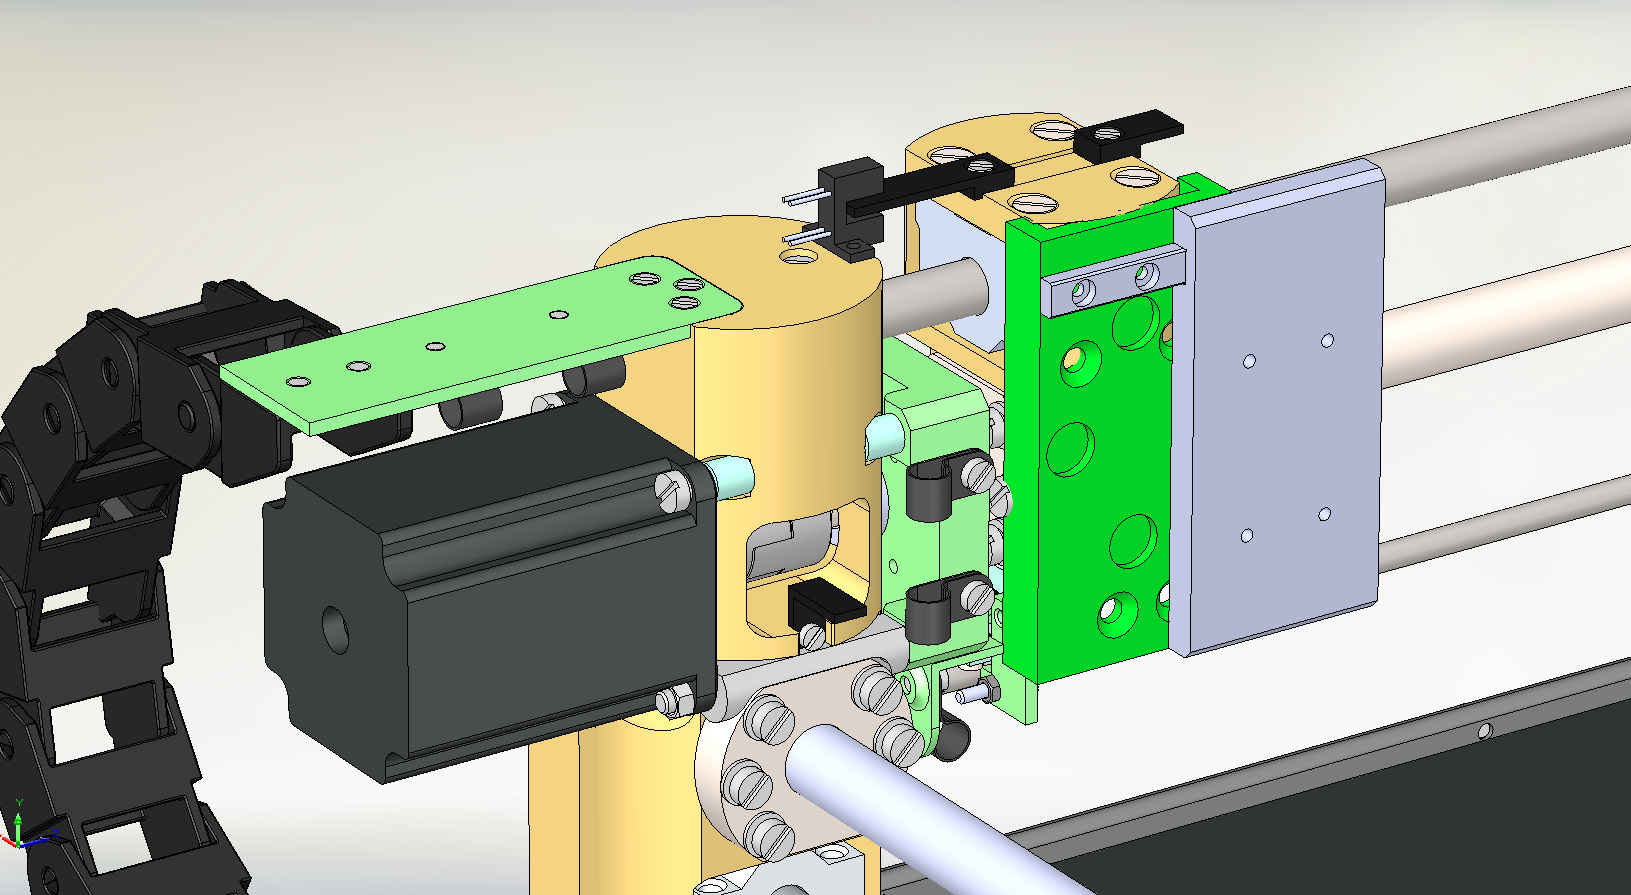
\includegraphics[width=0.7\textwidth]{ch-2/quick-mount}
	}
	\caption{Конструкция магнитного крепления модуля}\label{fig:quick-mount}
\end{figure}

\begin{figure}[ht]
	\centerfloat{
		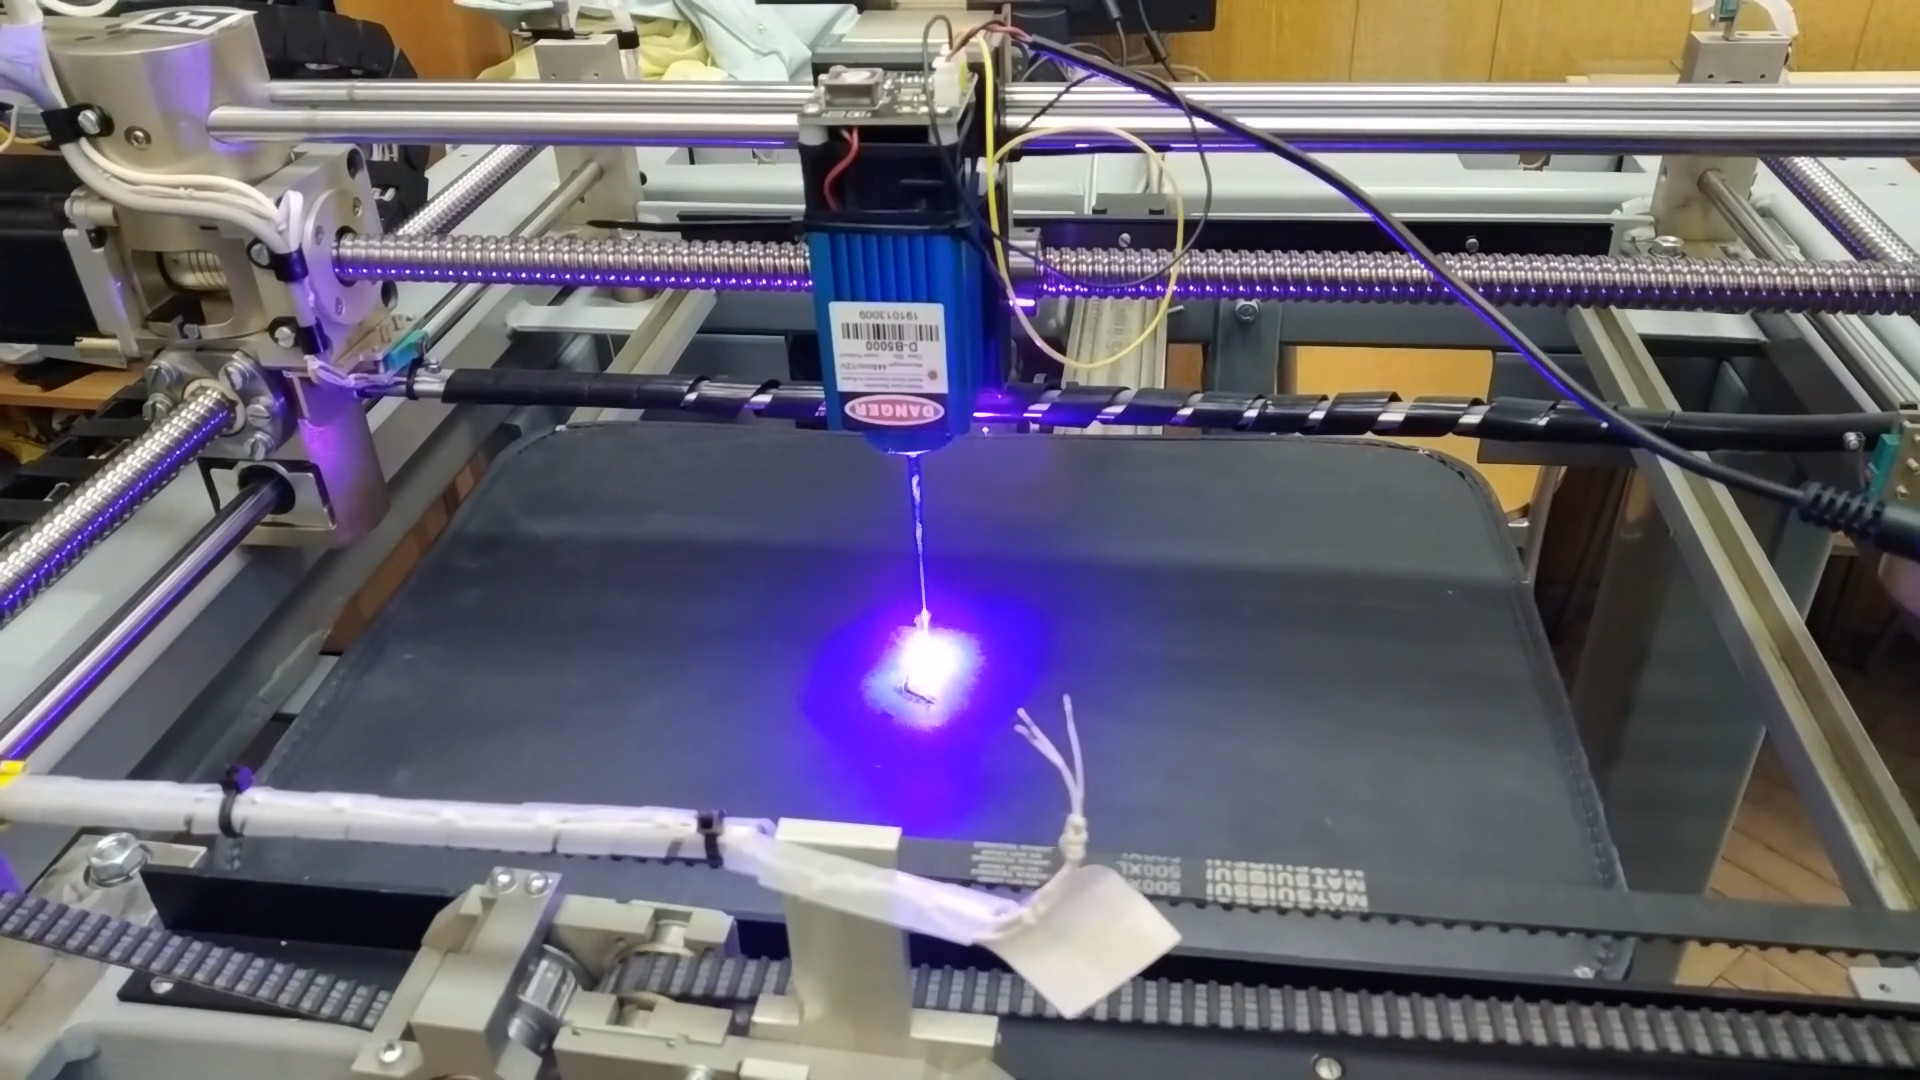
\includegraphics[width=0.7\textwidth]{ch-2/quick-mount-1}
	}
	\caption{Магнитного крепление с установленным лазерным модулем}\label{fig:quick-mount-1}
\end{figure}

\subsection{Этапы унификации модульного оборудования}

Первым этапом является определение параметров подлежащих унификации. Для модулей с электромагнитным креплением основными параметрами будут:

\begin{itemize}
	\item Грузоподъемность электромагнита.\footnote{Главный параметр.}
	\item Ширина присоединительной поверхности модуля. 
	\item Глубина модуля.
	\item Высота модуля.
	\item Ток потребления модуля.
\end{itemize}


Из данного списка необходимо выбрать главный параметр. Обычно главный параметр выбирают как параметр наиболее полно характеризующий несущую способность или другую эксплуатационную характеристику. Поскольку модули имеют различную функциональность, то в качестве главного параметра выбрана грузоподъемность электромагнита~\cref{eq-2-1}:

\begin{equation}
W = \{w_1, w_2, \ldots, w_n\}, n \in \mathbb{Z},
\label{eq-2-1}
\end{equation}

\noindent характеризующая выдерживаемое усилие. Этот параметр с одной стороны косвенно связан с массой модуля, а соответственно с возможностью его установки на каретку того или иного шасси. С другой стороны он может быть связан с технологическими режимами работы модуля, например с силой резания при фрезеровании.

Основные параметры обозначаются следующим образом~(рисунок~\cref{fig:geom-module}):

\begin{itemize}
	\item Ширина присоединительной поверхности модуля,\\$L = \{l_1, l_2, \ldots, l_n\}, n \in \mathbb{Z}$.
	\item Глубина модуля, $G = \{g_1, g_2, \ldots, g_n\}, n \in \mathbb{Z}$.
	\item Высота модуля, $H = \{h_1, h_2, \ldots, h_n\}, n \in \mathbb{Z}$.
	\item Ток потребления модуля, $I = \{i_1, i_2, \ldots, i_n\}, n \in \mathbb{Z}$.
\end{itemize}

\begin{figure}[tbh]
	\centering
	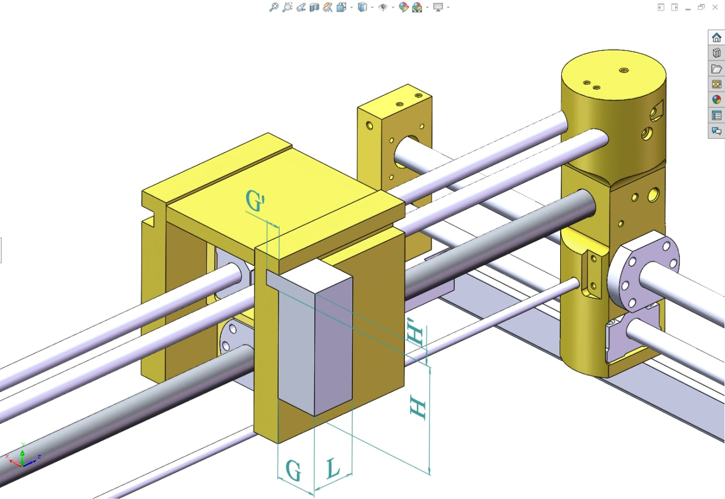
\includegraphics[width=\linewidth]{ch-2/geom-module}
	\caption{Параметры присоединительной поверхности модуля}
	\label{fig:geom-module}
\end{figure}

В качестве фиксированных параметров приняты:

\begin{itemize}
	\item Напряжение питания, $U$.
	\item Параметры ответной части паза, $G'$ и $H'$.
\end{itemize}

Напряжение питания выбрано в качестве фиксированного параметра, чтобы избежать применения преобразователей напряжения и использовать напряжение 24\:В де-факто ставшее промышленным стандартом. Параметры ответной части паза должны быть зафиксированы для обеспечения  широких возможностей по установке нескольких модулей одновременно. Следующим этапом необходимо определить ограничения выбранных параметров. Для модулей с электромагнитным креплением было выявлено пять ограничений.

\paragraph{Ограничение массы модуля в зависимости от грузоподъемности электромагнита.} При проектировании модуля необходимо учитывать его суммарную массу. Вес модуля должен быть меньше отрывного усилия в $\frac{1}{1-k}$ раз. Где $k$ "--- это коэффициент запаса. Формально ограничение может быть описано как~\cref{eq-2-1-1}:

\noindent $\rho : M \rightarrow P$ "--- соответствие <<модуль имеет массу>>.

\noindent $r : M \rightarrow W$ "--- соответствие <<электромагнит, установленный на модуль, имеет грузоподъемность>>.

\noindent $k$ "--- коэффициент запаса.

\begin{equation}
m \in M: k\rho(m) \leq r(m)
\label{eq-2-1-1}
\end{equation}

\paragraph{Ограничение грузоподъемности электромагнита в зависимости грузоподъемности шасси.} При проектировании модуля необходимо учитывать, что грузоподъемность электромагнита, а соответственно максимально устанавливаемая на шасси масса (масса модуля), должна была меньше грузоподъемности шасси c учетом коэффициента запаса~\cref{eq-2-2}.

\noindent $S = \{s_1, s_2, \ldots, s_n\}, n \in \mathbb{Z}$ "--- множество шасси.

\noindent $u: M \rightarrow S$ "--- соответствие <<модуль устанавливается  на шасси>>. 

\noindent $\vartheta: S \rightarrow P'$ "--- соответствие <<каретка шасси имеет грузоподъемность>> 

\begin{equation}
m \in M, s \in u(M): kr(m) \leq \vartheta(s)
\label{eq-2-2}
\end{equation}

Если предполагается устанавливать данный модуль одновременно с другими, то~\cref{eq-2-3}:

\begin{equation}
m \in M, s \in u(M): k\sum_{i=1}^{|M|}r(m_i) \leq \vartheta(s)
\label{eq-2-3}
\end{equation}

\paragraph{Ограничение тока потребления модуля в зависимости от максимального рабочего тока шасси.} Ток потребления модуля должен быть меньше рабочего тока шасси c учетом коэффициента запаса~\cref{eq-2-4}.

\noindent $M = \{m_1, m_2, \ldots, m_n\}, n \in \mathbb{Z} $ "--- множество модулей.

\noindent $i_{max} \in I$ "--- максимальный ток потребления.

\noindent $x: S \rightarrow i_{max}$ "--- <<соответствие шасси имеет максимальный рабочий ток>>.

\noindent $f: M \rightarrow I$ "--- соответствие <<модуль потребляет>>, тогда:

\begin{equation}
m \in M: kf(m) \leq x(s)
\label{eq-2-4}
\end{equation}

Если предполагается устанавливать данный модуль одновременно с другими, то~\cref{eq-2-5}:

\begin{equation}
m \in M: k\sum_{i=1}^{|M|}f(m_i) \leq x(s)
\label{eq-2-5}
\end{equation}

\paragraph{Ограничение глубины модуля в зависимости от рабочего пространства.} Глубина модуля определяет доступное рабочее пространство шасси в зависимости от общего рабочего поля шасси. С увеличением глубины модуля для обеспечения заданного рабочего пространства модуля необходимо увеличивать общее рабочее поле шасси. Тогда ограничение может быть записано как~\cref{eq-2-6}:

\noindent $S = \{s_1, s_2, \ldots, s_n\}, n \in \mathbb{Z} $ "--- множество шасси.

\noindent $G = \left \langle g_1, g_2, \ldots, g_n\right \rangle, n \in \mathbb{Z} $ "--- кортеж параметров глубины модулей.

\noindent $u: M \rightarrow S$ "--- <<соответствие модуль устанавливается на шасси>>.

\noindent $\delta: S \rightarrow B$ "--- соответствие <<шасси имеет размер рабочего пространства>>.

\noindent $y: M \rightarrow B'$ "--- соответствие <<для модуля задаётся минимальный размер рабочего пространства>>.

\noindent $\mu: M \rightarrow G$ "--- соответствие <<модуль имеет глубину>>.
 
\begin{equation}
m \in M, s \in u(M): \mu(m) + y(m) \leq \delta(s)
\label{eq-2-6}
\end{equation}

Если предполагается устанавливать данный модуль одновременно с другими, то~\cref{eq-2-7}:

\begin{equation}
m \in M, s \in u(M): max(\mu(M)) + y(m) \leq \delta(s)
\label{eq-2-7}
\end{equation}

\paragraph{Ограничение на ширину присоединительной поверхности модуля.} Необходимо уместить $n$ модулей с шириной присоединительной поверхности $l_{m_i} \in L$ на каретке шасси шириной $l_\omega$ компактно. Сущность критерия компактности заключается в том, чтобы оставшееся свободное пространство оставалось полезным, где под полезностью понимается возможность установить хотя бы один модуль.

\noindent Для обеспечения вместимости достаточно: $\sum_{i=1}^{n}l_{m_i} \leq l_\omega$.
\noindent Тогда критерий компактности определяется как~\cref{eq-2-8}: 

\begin{equation}
\left ( l_\omega - \sum_{i=1}^{n} l_{m_i} \right )\rightarrow 0
\label{eq-2-8} 
\end{equation}

\noindent и имеет свой оптимум при~\cref{eq-2-9}:

\begin{equation}
\sum_{i=1}^{n} l_{m_i} = l_\omega.
\label{eq-2-9}
\end{equation}

\noindent Тогда~\cref{eq-2-10}:

\begin{equation}
L' \subset L, L'' \subset L: \sum_{i=1}^{|L'|}l_m + \sum_{i=1}^{|L''|}l_m = l_\omega
\label{eq-2-10}
\end{equation}

Этому условию удовлетворяют кратные ряды вида~\cref{eq-2-11}:

\begin{equation}
\left \{ \ldots, \frac{l_\omega}{n^2}, \frac{l_\omega}{n^1}, \frac{l_\omega}{n^0} \right \}, n \in \mathbb{Z}
\label{eq-2-11}
\end{equation}


Последним этапом необходимо сформировать параметрические ряды. Для параметра грузоподъемности электромагнита можно использовать ряд предпочтительных чисел, при этом ряд должен быть ограничен сверху грузоподъемностью шасси~(\cref{eq-2-11-1}).

\begin{equation}
R10(\ldots \vartheta(s)),
\label{eq-2-11-1}
\end{equation}

\noindent где $\vartheta(s)$ "--- грузоподъемность шасси.


Параметрический ряд глубины модуля можно также сформировать из ряда предпочтительных чисел, при этом ряд должен быть ограничен сверху величиной равной разнице между рабочим поле шасси и минимальным желаемым размером рабочего поле модуля~\cref{eq-2-11-2}.

\begin{equation}
R10(\ldots \delta(s) - y(m)),
\label{eq-2-11-2}
\end{equation}

\noindent где $\delta(s)$ "--- длина рабочего пространства, $y(m)$ "--- минимальная длина рабочего пространства модуля.

Ряд параметра тока потребления можно выразить следующим образом~\cref{eq-2-11-3}:

\begin{equation}
R10(\ldots x(m)),
\label{eq-2-11-3}
\end{equation}
						
\noindent гед $x(s)$ "--- рабочий ток шасси.

Параметр ширины присоединительной поверхности не может быть выбран из  ряда предпочтительных чисел, поскольку это не гарантирует обеспечения компактности. Тогда, исходя из критерия компактности можно синтезировать кратные ряды вида~\cref{eq-2-11}: 

Используя полученные параметрические ряды, появляется возможность добиться совместимости разрабатываемого модуля с шасси и модулями других разработчиков, при этом не имея описания и документации на объекты совместимости. Кроме этого возможно достижение опережающей совместимости с объектами разработанными в будущем. На основе полученного формального описания рядов создана параметрическая модель для автоматизированных систем проектирования SolidWorks и OpenSCAD, позволяющая упростить проектирование модулей благодаря автоматическому расчёту параметров и проверки совместимости~(рисунок~\cref{fig:param}).

\begin{figure}[ht]
	\centerfloat{
		\hfill
		\subcaptionbox{\label{fig:param-1}}{%
			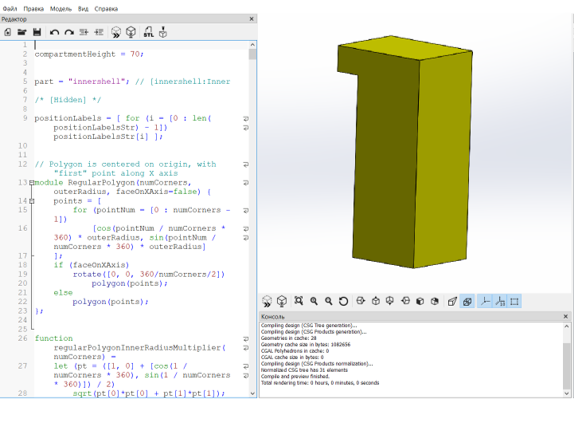
\includegraphics[width=0.49\linewidth]{ch-2/openscad}}
		\hfill
		\subcaptionbox{\label{fig:param-2}}{%
			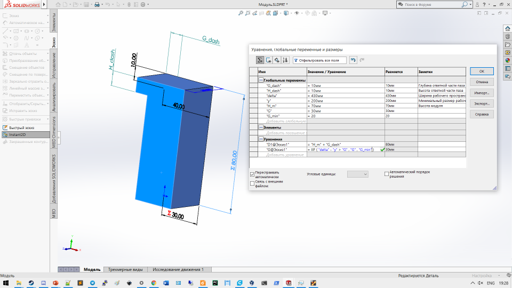
\includegraphics[width=0.49\linewidth]{ch-2/solidworks}}
		\hfill
	}
	\caption[Примеры эскизов моделей, созданных на основе параметрических рядов]%
	{Примеры эскизов моделей, созданных на основе параметрических рядов: в системе автоматизированного проектирования OpenSCAD (\textit{а}), в системе автоматизированного проектирования SolidWorks (\textit{б}).}\label{fig:param}
\end{figure}

\section{Показатель целесообразности применения модульного оборудования}

Особенностью частных малых предприятий, занимающихся производством, является повышенная осторожность внедрения новых технологий и подходов. Зачастую это рассматривается как неоправданный, сложно поддающийся прогнозу риск, поскольку достаточно сложно произвести предварительную оценку целесообразности применения того или иного новшества, а также определить готовность предприятия к внедрению. Обычно задача предварительной оценки внедрения новшества лежит исключительно в экономической плоскости. Рассчитываются такие показатели как индекс рентабельности (PI), срок окупаемости (PBP), внутренняя оценка доходности (IRR) и т.\:д. При этом величины параметров, на которые опираются показатели,  основываются на экспертных оценках. Все вышесказанное касается и внедрения новых видов технологического оборудования. Одним из самых распространенных способов общей оценки эффективности оборудования является показатель OEE~\cite{oee}.\footnote{Сокр. от англ.~\textit{Overall Equipment Effectiveness} "--- общий эффективность оборудования.}

Общая эффективность оборудования (OEE) позволяет получить представление об общей производительности предприятия. Данная метрика стала развитием критерия Total Productive Maintenance (сокр. \textit{TPM}). OEE "--- это общее рассчитанное значение, которое представляет эффективность предприятия по трем ключевым показателям производительности:

\begin{itemize}
	\item Доступность оборудования, то есть возможность использования его в производственном процессе.
	\item Производительность, то есть количество выпускаемой продукции в единицу времени без учёта брака.
	\item Приведённый уровень качества. 
\end{itemize}

\textit{Коэффициент доступности}. Это фактическое время выполнения технологических операций в течение определенного интервала времени, деленное на <<запланированное>> время выполнения для того же интервала. Например, работы, которые запланированы с учётом длительности рабочей смены, равной 8 часам в день, 5 дней в неделю, имеет общую доступность 40 часов. Если фактическое время работы составляет 20 часов, результирующий коэффициент доступности составляет 50\,\%.

\textit{Производительность} "--- это фактическая валовая единица продукции, произведенная за определенный промежуток времени, деленная на количество единиц, которые должны были быть произведены. Технически, знаменатель в этом случае должен быть идеальным показателем, определяемы технологической документацией, но в большинстве случаев возможно увеличение производительность по сравнению с первоначальной <<паспортной>> производительностью.

\textit{Показатель качества} является достаточно простым критерием. Это общее количество произведенных единиц продукции без брака, разделенное на общее количество произведенных единиц. Общее количество единиц продукции без брака определяется как общее количество произведенных единиц (брутто) за вычетом всего брака, как устранимого, так и неустранимого. Например, если производится всего 1000 единиц, но 100 единиц продукции отбраковываются, то числитель становится 900, а знаменатель "--- 1000, что даёт значение коэффициента равным~90\,\%.

Таким образом, после определения этих трех значений окончательный расчет OEE представляет собой произведение трёх значений, выраженных в процентах, то есть "--- это мультипликативный показатель который включает в себя три критерия~\cref{eq:oee}:\footnote{Электронный ресурс: \url{https://www.oee.com/} (дата обращения: 14.06.2019).}

\begin{equation}
OEE = A \times P \times Q,
\label{eq:oee}
\end{equation} 

\noindent где:

\noindent $A$ "--- критерий доступности (готовности) оборудования (англ. \textit{Availability});

\noindent $P$ "--- критерий производительности (англ. \textit{Performance});

\noindent $Q$ "--- критерий качества (англ. \textit{Quality})

Критерий доступности позволяет оценить простои оборудования, которые с одной стороны могут быть связаны с поломками, а с другой стороны "--- неравномерностью потока заказов. Для мелкосерийного и единичного дискретного производства, которые зачастую работают по принципу ETO\footnote{Сокр. от англ. \textit{Engineer-To-Order} "--- заказ на проектирование.} или MTO\footnote{Сокр. от англ. \textit{Made-To-Order} "--- заказ на изготовление.}, а не производят продукцию на склад, неравномерность потока заказов может привести к простою части оборудования.

Необходимо отметить особенности этих двух подходов к изготовлению продукции на заказа. MTO "--- производственный подход, при котором после получения подтвержденного заказа на продукты начинается полный производственный цикл их изготовления. Этот подход считается подходящим для продуктов с высокой степенью конфигурации, таких как автомобили, компьютерные серверы, или для продуктов, хранение запасов которых обходится дорого, например самолетов. MTO является основным подходом, используемый сегодня во многих отраслях. Он относится к изделиям, созданным до определения конечного покупателя, при этом объём производства определяется \textit{исторической информацией о спросе}.

Основными преимуществами подхода MTO в среде с большим разнообразием продуктов являются возможность предоставить заказчику точную требуемую спецификацию продукта, сокращение дорогостоящих товарных запасов, а также снижение риска устаревания запасов.
Основным недостатком MTO является то, что производители чувствительны к колебаниям рыночного спроса, что ведет к снижению загрузки производственных мощностей в производстве. Следовательно, для обеспечения эффективного использования производственных ресурсов подход MTO должен сочетаться с упреждающим управлением спросом, что является актуальной областью научных исследований.

С другой стороны, ETO "--- это производственный подход, обладающий следующими особенностями:

\begin{itemize}
	\item К срокам выполнения заказа следует добавить инженерные работы.
	\item После получения заказа от клиента технические требования и спецификации заказа в деталях не известны. Требуется значительный объем проектного и инженерного анализа.
\end{itemize}

ETO "--- это эффективный метод увеличения продаж и увеличения прибыльности для тех компаний, клиенты которых нуждаются в индивидуальных решениях, соответствующих их уникальным требованиям. Он начинается с продажи концепций продуктов, которые не имеют готового проекта и, как ожидается, позволят создать новый уникальный конечный продукт. Это может быть любой продукт, от корпоративных программных приложений до изделий машиностроения. Тем не менее, типичная среда ETO обычно имеет дело с проектированием и сборкой сложных машин и промышленного оборудования, спроектированных по индивидуальному заказу.

И последний критерий, "--- критерий качества, "--- позволяет оценивать уровень брака выпускаемой продукции~\cref{eq:oee-3}.

\begin{equation}
	Q = \frac{GP}{TP}
	\label{eq:oee-3}
\end{equation}

\noindent где:

\noindent $GP$ "--- количество годной продукции, выпущенное за операционное время,
\noindent $TP$ "--- общее количество продукции, выпущенное за операционное время.

Учитывая вышесказанное, очевидно, что использовать показатель OEE имеет смысл только после внедрения оборудования и оценки целесообразности применения его постфактум. Однако для текущей оценки эффективности работы оборудования данный показатель незаменим. Положительным считается результат величиной больше 0,75, а отрицательным меньше значения 0,65.\footnote{Электронный ресурс: \url{promanage.com/7-blog/956-how-to-improve-oee/} (дата обращения 08.04.2020).} В случае неудовлетворительной оценки, где наибольший негативный эффект вносят составляющие критерия доступности и критерия производительности применение модульного оборудования позволяет привести к повышению значения OEE. Это связано с тем, что снижение производительности и доступности оборудования, вызывается образованием узких мест на производстве. При изготовлении деталей технологические операции имеют различную длительность. В случае, когда одна или несколько технологических операций при обработке партии деталей имеют большую по сравнению с остальными операциями продолжительность, оборудование начинает простаивать в ожидании предмета труда. В данных обстоятельствах модульное оборудование позволяет избавиться от узкого места меньшими затратами на дополнительное оборудование, за счет возможности временной реконфигурации других простаивающих единиц оборудования. 

Тем не менее, проведение анализа системы на наличие узких мест является трудоемким процессом, требующим временных затрат на сбор данных о функционировании системы. А в случае с новыми производственным предприятиями такую информации получить невозможно из-за отсутствия полноценно функционирующего производства. При этом одним из этапов планирования нового производства является определение перечня необходимых ресурсов, куда включается технологическое оборудование. Для вышеуказанных целей предлагается использование \textit{показателя целесообразности модульности}. 

Для расчета показателя целесообразности модульности необходимо получить данные о номенклатуре производимых деталей. Для мелкосерийного и единичного производства эту информацию можно получить из имеющихся маршрутных карт групповых технологических процессов. Представим номенклатуру в виде множества~$N$~\cref{eq-2-15}:

\begin{equation}
N = \{D_1, D_2, \ldots, D_i\}, N = (D_i)_{i \in \mathbb{Z}},
\label{eq-2-15}
\end{equation}


где $D_i$ "--- это групповая деталь, представляющая собой множество классов технологических операций $p_m$ по классификатору технологических операций машиностроения и приборостроения~\cref{eq-2-16}:\footnote{Классификатор технологических операций машиностроения и приборостроения: 1 85 151. М.: Издательство стандартов, 1987.}

\begin{equation}
D = \{p_1, p_2, \ldots, p_m\},
\label{eq-2-16}
\end{equation}

\noindent В соответствие каждой групповой детали указывается планируемый объем выпуска~\cref{eq-2-17}:

\begin{equation}
f: D \rightarrow v_i, V \in \mathbb{Z}
\label{eq-2-17}
\end{equation}

На следующем этапе необходимо определить групповые детали с максимальным объемом выпуска (это может быть одна деталь или несколько). Данную процедуру представим в виде композиции функций~\cref{eq-2-18}:

\begin{equation}
\begin{split}
f &\circ g, \\
g: V \rightarrow N'': \forall v &= V_max f(D), v \in V, \\
\end{split}
\label{eq-2-18}
\end{equation}

%\begin{equation}
%f \circ g,
%\end{equation}
%
%\begin{equation}
%g: V \rightarrow N'': \forall v = V_max f(D), v \in V,
%\end{equation}

\noindent где $V$ "--- кортеж, содержащий значения объемов выпуска для каждого вида изделий. Тогда $G=({N''}_i)_{i \in J}$ -- это семейство групповых деталей с максимальным объемом выпуска.
%ЧТО ТАКОЕ J?
Отсюда коэффициент целесообразности будет можно выразить следующим образом~\cref{eq-2-19}:

\begin{equation}
\epsilon = \frac{\big|\bigcup G \big|}{\big|\bigcup N \big|}
\label{eq-2-19}
\end{equation}

\noindent при $\epsilon \rightarrow 1$, модульность нецелесообразна.

\noindent при $\epsilon \rightarrow 0$, модульность целесообразна.

\paragraph{Описание маршрутного технологического процесса изделия <<Гироподвес>>.}

В качестве примера был рассмотрен технологический процесс изготовления изделия <<Гироподвес>>. Выбор был обусловлен тем фактом, что вся конструкторская документация на данное изделие находится в свободном доступе и может быть использована для создания и оптимизации маршрутной технологии для модульного технологического оборудования. Расчетные параметры технологических операций данного технологического процесса будут использоваться в оставшихся разделах данной главы.

Изделие <<Гироподвес>>~(рисунок~\cref{fig:gimbal}) представляет собой подвижную платформу, на которой может быть закреплена камера. Задача данного изделия "--- стабилизировать положение камеры по осям крена, тангажа и рысканья. Изделие состоит из следующих узлов:

\begin{itemize}
	\item Пластиковые корпусные детали, которые могут быть распечатаны на установке послойного наплавления (трёхмерном принтере)~(рисунок~\cref{fig:gimbal-1}).\footnote{Электронный ресурс: \url{https://www.thingiverse.com/thing:1247236} (дата обращения: 16.03.2020).} 
	\item Печатная плата~(рисунок~\cref{fig:gimbal-2}).\footnote{Электронный ресурс: \url{https://github.com/olliw42/storm32bgc} (дата обращения: 26.07.2020).}
	\item Стандартные и покупные изделия.
\end{itemize}

\begin{figure}[htb]
	\centerfloat{
		\hfill
		\subcaptionbox{\label{fig:gimbal-1}}{%
			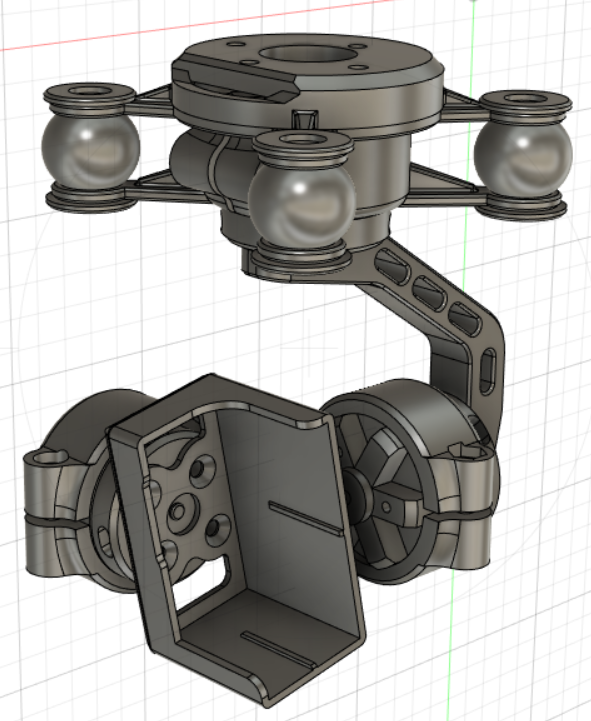
\includegraphics[width=0.33\linewidth]{ch-2/gimbal-3d}}
		\hfill
		\subcaptionbox{\label{fig:gimbal-2}}{%
			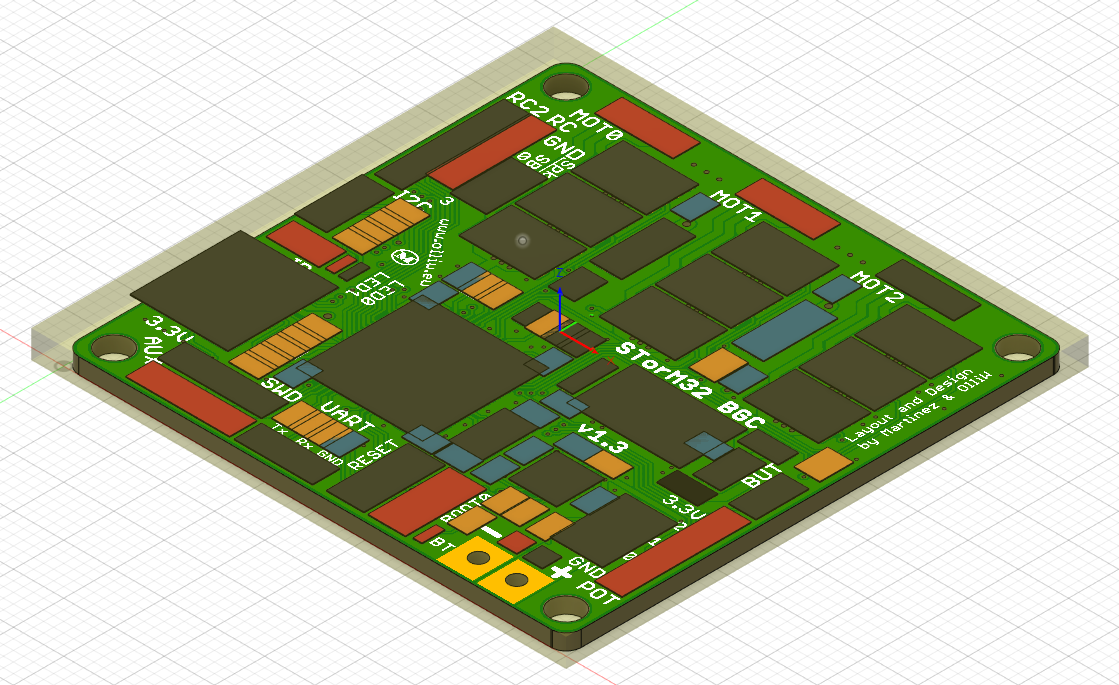
\includegraphics[width=0.33\linewidth]{ch-2/gimbal-pcb}}
		\hfill
		\subcaptionbox{\label{fig:gimbal-3}}{%
			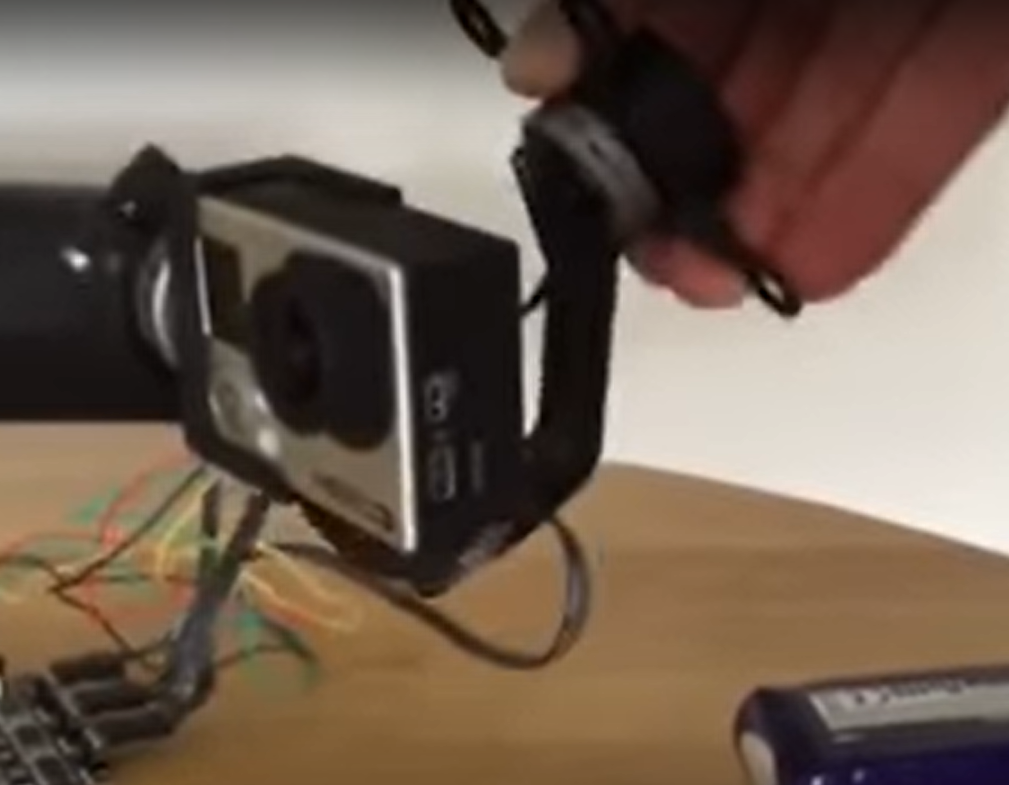
\includegraphics[width=0.33\linewidth]{ch-2/gimbal}}
		\hfill
	}
	\caption[Изделие <<Гироподвес>>]%
	{Изделие <<Гироподвес>>: трёхмерная модель (\textit{а}), печатная плата  (\textit{б}), готовое изделие (\textit{в}).}\label{fig:gimbal}
\end{figure}

Последовательность операций изготовления корпусных деталей на установке послойного наплавления представлена в таблице~\cref{tab:case}, последовательность изготовления печатной платы представлена в таблице~\cref{tab:pcb}.\footnote{Маршрутная карта представлена в приложении~\cref{app:A}.}

\begin{table} [!htb]
	\centering
	\caption{Последовательность операций изготовления корпусных деталей изделия <<Гироподвес>>} \vspace{4pt}
	\label{tab:case}
	\begin{threeparttable}
		\begin{tabularx}{\linewidth}{ll}
			\toprule
			\textbf{Код операции\tnote{1}} & \textbf{Наименование операции} \\
			\midrule
			6051 & Экструзия заготовок \\
			0108 & Слесарная \\ 
			4232 & Сверлильная с ЧПУ \\
			\bottomrule
		\end{tabularx}
		\begin{tablenotes} \footnotesize
			\item [1] Код из классификатора операций 1 85 151.
		\end{tablenotes}
	\end{threeparttable}
\end{table}

\begin{table} [!htb]
	\centering
	\caption{Последовательность операций изготовления печатной платы изделия <<Гироподвес>>} \vspace{4pt}
	\label{tab:pcb}
	\begin{threeparttable}
		\begin{tabularx}{\linewidth}{ll}
			\toprule
			\textbf{Код операции\tnote{1}} & \textbf{Наименование операции} \\
			\midrule
			4232 & Сверлильная с ЧПУ \\
			0109 & Зачистка \\
			0191 & Обезжиривание химическое \\
			6077 & Ламинирование пленочного фоторезиста \\
			5541 & Экспонирование \\
			5545 & Проявление \\
			0151 & Травление химическое \\
			0195 & Удаление покрытий \\
			6077 & Ламинирование паяльной маски \\
			5541 & Экспонирование \\
			5545 & Проявление \\
			0127 & Промывка растворителями \\
			6077 & Ламинирование трафаретных чернил \\
			5541 & Экспонирование \\
			5545 & Проявление \\
			0127 & Промывка растворителями \\
			4234 & Фрезерная с ЧПУ \\
			0158 & Дозирование по объему \\
			8878 & Монтаж комплектующих изделий \\ 
			8035 & Пайка готовым припоем в нейтральной газовой среде в печи \\
			\bottomrule
		\end{tabularx}
		\begin{tablenotes} \footnotesize
			\item [1] Код из классификатора операций 1 85 151.
		\end{tablenotes}
	\end{threeparttable}
\end{table}

\paragraph{Пример расчета коэффициента целесообразности.}

На производстве имеется 3 маршрутные карты групповых технологических процессов:

\begin{itemize}
	\item Маршрутная карта изготовления пластикового корпуса методом послойного наплавления, объём выпуска 100 единиц в год ($D_{case}$).
	\item Маршрутная карта изготовления печатной платы, объём выпуска 300 единиц в год ($D_{pcb}$).
	\item Маршрутная карта изготовления печатной платы с поверхностным монтажом электронных SMD-компонентов, объём выпуска 200 единицы в год~($D_{smd}$).
\end{itemize}

Здесь и далее четырёхзначные числа в скобках означают коды операций в классификаторе операций~\cref{eq-2-20}.

\begin{equation}
\begin{split}
	N &= \{D_{case}, D_{cb}, D_{smd}\} \\
	D_{case} &= \{005, 010\} \\
	D_{pcb} &= \{010, 015\} \\
	D_{smd} &= \{010, 015, 020, 025\}
\end{split}
\label{eq-2-20}
\end{equation}

\noindent Тогда~\cref{eq-2-21}:

\begin{equation}
\begin{split}
G &= (\{010, 015\}) \\
\bigcup G &= (\{010, 015\}) \\
\bigcup N &= \{005, 010, 015, 020, 025\} \\
\epsilon &= \frac{\big|\bigcup G \big|}{\big|\bigcup N \big|} = \frac{2}{5} = 0,25
\end{split}
\label{eq-2-21}
\end{equation}

Учитывая полученное значение, можно сделать ввод о целесообразности применения модульного оборудования. Для проверки достоверности результата был проведен вычислительный эксперимент в системе Anylogic. Групповой технологический процесс изготовления печатной платы был представлен в виде диаграммы процесса с помощью дискретно-событийного метода.\footnote{Электронный ресурс: \url{https://www.anylogic.ru/use-of-simulation/discrete-event-simulation/} (дата обращения: 13.12.2018)} При этом было построено две диаграммы: для процесса использующего модульное оборудование~(рисунок~\cref{fig:oee-module-1}) и использующего немодульное оборудование (рисунок~\cref{fig:oee-module-2}).

\begin{figure}[!p]
	\centerfloat{
		\hfill
		\subcaptionbox{\label{fig:oee-module-1}}{%
			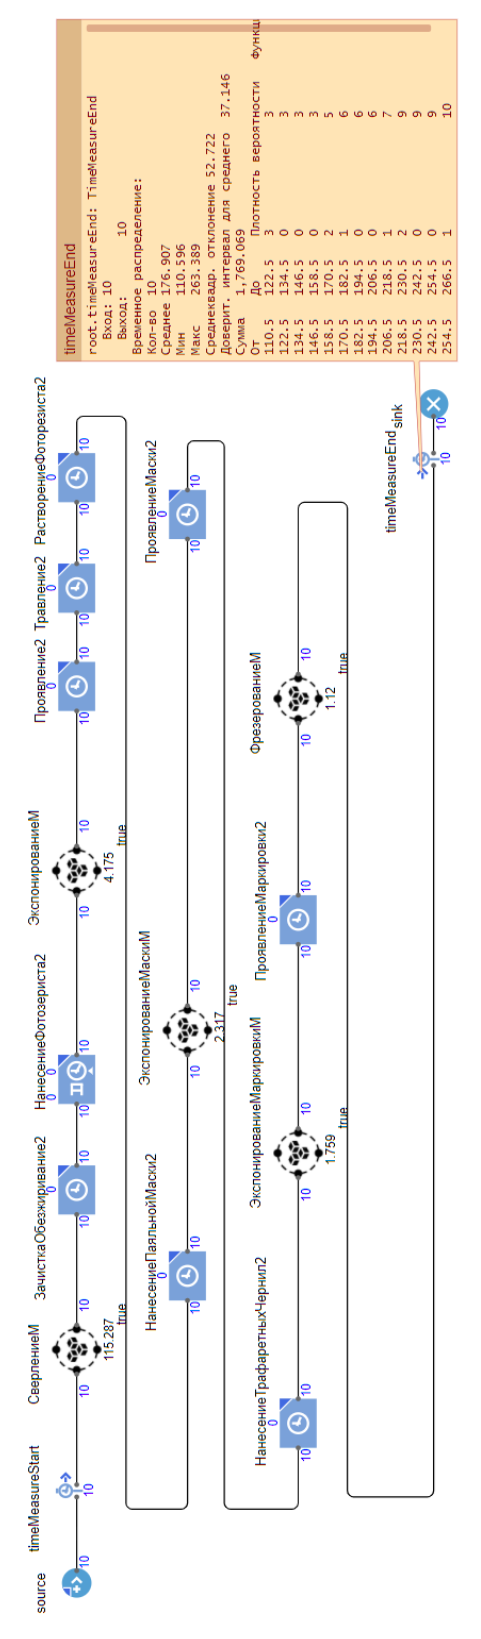
\includegraphics[width=0.42\linewidth]{ch-2/oee-module}}
		\hfill
		\subcaptionbox{\label{fig:oee-module-2}}{%
			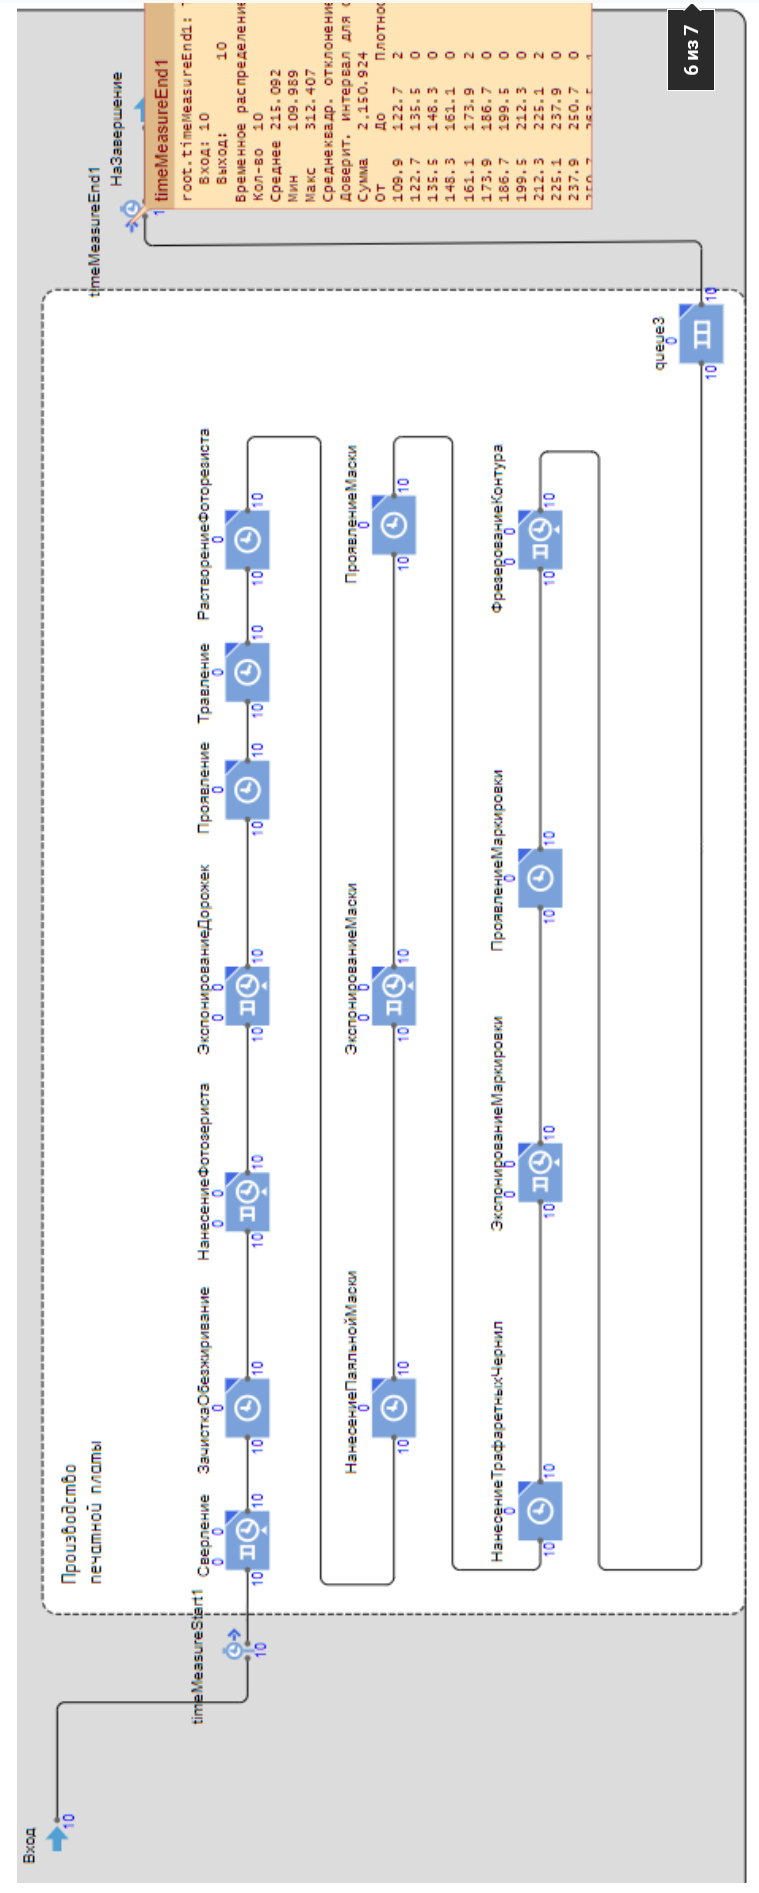
\includegraphics[width=0.52\linewidth]{ch-2/oee-no-module}}
		\hfill
	}
	\caption[Диаграмма процесса производства печатной платы для модульного и немодульного оборудования]%
	{Диаграмма процесса производства печатной платы для модульного (\textit{а}) и немодульного (\textit{б}) оборудования}\label{fig:oee-module}
\end{figure}

В процессе симуляции было обнаружено узкое место процесса на операции <<сверление>>, поскольку длительность её выполнения превосходила все остальные операции. Для повышения производительности, а соответственно снижения времени технологического цикла было предложено увеличить количество сверлильного оборудования. Для немодульного оборудования необходимо было добавить два дополнительных сверлильных станка, в то время как для модульного подхода было добавлено два сверлильных модуля, а шасси были переконфигурированы с простаивающих установок печати, монтажа и дозирования. В результате был получен прирост производительности в~\SI{18}{\percent}. Результаты вычислительного эксперимента представлены в таблице~\cref{tab:mod-nomod}.

\begin{table} [!htb]
	\centering
	\caption{Длительность технологического цикла производства партии печатных плат объёмом 10 единиц} \vspace{4pt}
	\label{tab:mod-nomod}
	\begin{threeparttable}
		\begin{tabularx}{\linewidth}{llr}
			\toprule
			\textbf{Тип оборудования} & \textbf{Перечень оборудования}    & \textbf{Время, мин.} \\
			\midrule
			Модульное                 & \begin{tabular}{@{}l@{}}
											3 сверлильных станка\\ 
											1 установка экспонирования\\
											1 фрезерный станок
										\end{tabular}                     & 29,5 \\
			Немодульное               & \begin{tabular}{@{}l@{}}
											1 модуль экспонирования\\       
											1 модуль фрезерования\\
											3 модуль сверления\\
											6 шасси\tnote{1}
										\end{tabular}                     & 36 \\	
			\bottomrule
		\end{tabularx}
		\begin{tablenotes} \footnotesize
			\item [1] Три единицы шасси снимаются с простаивающих установок печати, монтажа и дозирования.
		\end{tablenotes}
	\end{threeparttable}
\end{table}


\section{Оптимизация комплектов модульного технологического оборудования}
	 
\subsection{Определение требований к комплектам модульного технологического оборудования и задачи оптимизации}

Комплектом технологического оборудования называется часть парка оборудования предприятия, используемая для реализации конкретного технологического процесса. Под парком технологического оборудования понимается совокупность оборудования, выполняющего технологические операции в автоматизированном режиме на одном предприятии. Парк технологического оборудования -- это важный производственный ресурс, определяющий такие характеристики производственного процесса как производительность, стоимость и качество выходной продукции. При этом производительность определяется с одной стороны производительностью каждой единицы оборудования по отдельности, а с другой, количеством единиц оборудования, работа которых может осуществляться параллельно.  Вместе с этим, оборудование -- это один из самых дорогостоящих ресурсов, требующий значительных затрат как на начальном этапе организации производства, так и в процессе эксплуатации. На данный момент наиболее дорогостоящим остается технологическое оборудование с ЧПУ. Это связано с рядом причин:

\begin{itemize}
	\item Высокая стоимость приводов движущей части технологического оборудования, особенно в случае применения сервоприводов.
	\item Сложность реализации системы управления, алгоритмы которой зачастую засекречены производителями.
	%* -- что-то еще? --
\end{itemize}

При организации парка оборудования важно, чтобы он отвечал следующим требованиям:

\begin{itemize}
	\item Обеспечение достаточного уровня автоматизации, соответствующего современным достижениям в науке и технике, в том числе использование ЧПУ.
	\item Обеспечение постепенного обновления имеющегося парка технологического оборудование.
	\item Применение производительных способов обработки.
	\item Гибкость парка оборудования при смене объемов и номенклатуры производства.
	\item Высокая отказоустойчивость.
\end{itemize}

Формирование парка оборудования это комплекс мероприятий, требующий точно определить и обосновать величину потребности в технологическом оборудовании, поскольку как недостаток, так и излишнее количество оборудования оказывают негативный эффект. Недостаточное количество технологического оборудования  приводит к ряду негативных эффектов:

\begin{itemize}
	\item Образованию узких мест.
	\item Повышенной загруженности определенных единиц оборудования.
	\item Простою определенных единиц оборудования в ожидании предмета труда для обработки.
	\item Межоперационное пролеживание предметов труда.
	\item Низкая отказоустойчивость.
\end{itemize}


Наряду с этим, излишнее количество также влечет к образованию простоев из-за малой загрузки и дополнительным финансовым издержкам. 

Учитывая вышесказанное, становится очевидной необходимость решения задачи оптимизации комплекта технологического оборудования, которая заключается в определении оптимального количества необходимых единиц оборудования.

Комплект модульного технологического оборудования может как формировать комплект технологического оборудования полностью, так и только его часть. Предлагаемое модульное технологическое оборудование строится на основе базового агрегата, "--- координатного шасси, "--- отвечающего за перемещение каретки и установленных на неё модулей. Управление происходит также как и у немодульного оборудования с ЧПУ с помощью G-код программ и коротких команд. Применение электромагнитного крепления модулей и программного обеспечения с автоматической инициализацией и установкой связью с шасси позволяет не тратить большое количество времени на реконфигурацию машин. Отсюда наблюдается тенденция такого оборудования:

\begin{itemize}
	\item К повышению гибкости комплекта оборудования за счет возможной быстрой реконфигурации единиц модульного технологического оборудования.
	\item К повышению отказоустойчивости за счет возможной быстрой реконфигурации простаивающего оборудования.
	\item К повышению производительности меньшим эквивалентным количеством модульного оборудования, чем немодульного оборудования.
\end{itemize}

Тогда в случае с модульным технологическим оборудованием задача оптимизации конкретизируется как задача определения оптимального количества шасси и модулей для одного или нескольких технологических процессов.

\subsection{Целевая функция оптимизации комплекта модульного технологического оборудования}\label{sec:target-func}

Оптимизация "--- это выбор наилучшего варианта из возможных на основе одного или нескольких критериев. Для оптимизации комплекта модульного технологического оборудования необходимо рассматривать два критерия "--- стоимость предлагаемого комплекта оборудования и длительность технологического цикла. Фактически задача оптимизации сводится к задаче двухкритериальной оптимизации, где оба вышеуказанных критерия должны подвергаться минимизации.

Решение задач многокритериальной оптимизации является достаточно сложным и ресурсоёмким, поэтому по-возможности сводится к переходу от многокритериальной задачи к однокритериальной. Такой переход осуществляется за счет свертки. Самым распространенным способом свертки является аддитивная свертка\footnote{Васильев В.\,П., Мельник А.\,О. Решение многокритериальных задач принятия решения посредством смешанной свертки критериев //Современные инновационные технологии и проблемы устойчивого развития общества. "--- 2018. "--- С. 163-168.}, основанная на принципе взаимных компенсаций. Однако для обеспечения корректной компенсации критерии с разными единицами измерения следует нормировать.
 
Предлагается целевая функция оптимизации модульного технологического оборудования следующего вида~\cref{eq-2-22}:

\begin{equation}
F(t, c, \{m_1, m_2, \ldots m_n \}) = k_t \cdot \frac{t}{t_{norm}} + k_c \cdot \frac{c}{c_{norm}} + \sum_{i=0}^{n}k_i \cdot m_i, n \in \mathbb{Z},
\label{eq-2-22}
\end{equation}

\noindent где:
\noindent $k_t$, $k_c$, $k_i$ "--- весовые коэффициенты,
\noindent $t$ "--- время технологического цикла,
\noindent $t_{norm}$ "--- нормирующий множитель времени технологического цикла,
\noindent $с$ "--- количество шасси,
\noindent $c_{norm}$ "--- нормирующий множитель количества шасси,
\noindent $m_i$ "--- количество модулей определенного типа,\footnote{Модули относятся к одному типу, если выполняют операции одного класса.} выполняющих операцию определенного класса.

В качестве нормирующего множителя $t_{norm}$ используется длительность технологического цикла, рассчитанного для случая, где количество шасси соответствует количеству типов модулей, а количество модулей каждого типа принято за единицу. В качестве нормирующего множителя $c_{norm}$ используется количество шасси равное количеству типов модулей.

\subsection{Расчёт весовых коэффициентов}\label{sec:weight}

Весовые коэффициенты необходимы для того, чтобы указать степень важности того или иного критерия в свертке. Зачастую для получения значений весовых коэффициентов прибегают к экспертной оценки, с использованием различных методов: метода анализа иерархий, метода парного сравнения, метода ранжирования, метода приписывания баллов и т.\,д. Основная сущность этих методов сводятся к переводу качественной оценки эксперта или группы экспертов в некоторое числовое значение.  Однако весовые коэффициенты полученные по таким методам могут носить субъективный характер, а для достижения необходимой степени объективности потребуется найти и привлечь большое количество профильных специалистов.

Отсутствие формальных методов связано с сильной привязкой значений весовых коэффициентов с предметной областью их использования. В работе предлагается проводить расчёт весовых коэффициентов на основе удельных весов каждого критерия от стоимостного показателя на базе годовой выручки~\cref{eq-2-23}:

\begin{equation}
\begin{split}
	w   &= s_{one} \cdot \frac{t_{year}}{t_{one}} - s_c - \sum s_i \\
	k_c &= \frac{s_c}{w} \\
	k_i &= \frac{s_i}{w} \\
	k_t &= s_{one} \cdot \frac{t_{year}}{t_{one} \cdot w}
\end{split}
\label{eq-2-23}
\end{equation}

\noindent где:
\noindent $w$ "--- разница между годовой выручкой и издержками на модули и шасси,
\noindent $t_{year}$ "---количество рабочих часов в году,
\noindent $t_{one}$ "--- норма штучного времени,
\noindent $s_{one}$ "--- стоимость одной детали,
\noindent $s_i$ "--- стоимость модуля определенного типа,
\noindent $s_c$ "--- стоимость шасси.

\subsection{Алгоритм оптимизации}

Наиболее прямолинейным алгоритмом оптимизации является алгоритм прямого перебора значений количества шасси и модулей с последующий оценкой величины целевой функции. Однако даже при ограничении количества шасси и модулей максимальным порогом, количество итераций может достигать значительных размеров. Поэтому предлагается алгоритм оптимизации, основанный на компенсации узких мест.

Суть алгоритма заключается в итерации от главной операции (зачастую являются узким местом) к остальным операциях, сопровождающейся добавлением шасси и модулей, а затем оценкой значения целевой функции. Главной операцией считается операция с наибольшей длительностью. Входными данными алгоритма являются:

\begin{itemize}
	\item Последовательность длительностей технологических операций в виде списка (\texttt{operations[]}).
	\item Пределы значений количества шасси и модулей (\texttt{chassis\_limit, modules\_limit[]}).
	\item Размер партии (\texttt{batch}).
\end{itemize}


Выходными данными алгоритма являются:
\begin{itemize}
	\item количество шасси (\texttt{chassis\_n})
	\item количество модуля каждого вида в виде списка (\texttt{modules\_n[]})
\end{itemize}


Рассмотрим блок-схему алгоритма~(рисунок~\cref{fig:algo-1}).

\begin{figure}[!b]
	\centerfloat{
		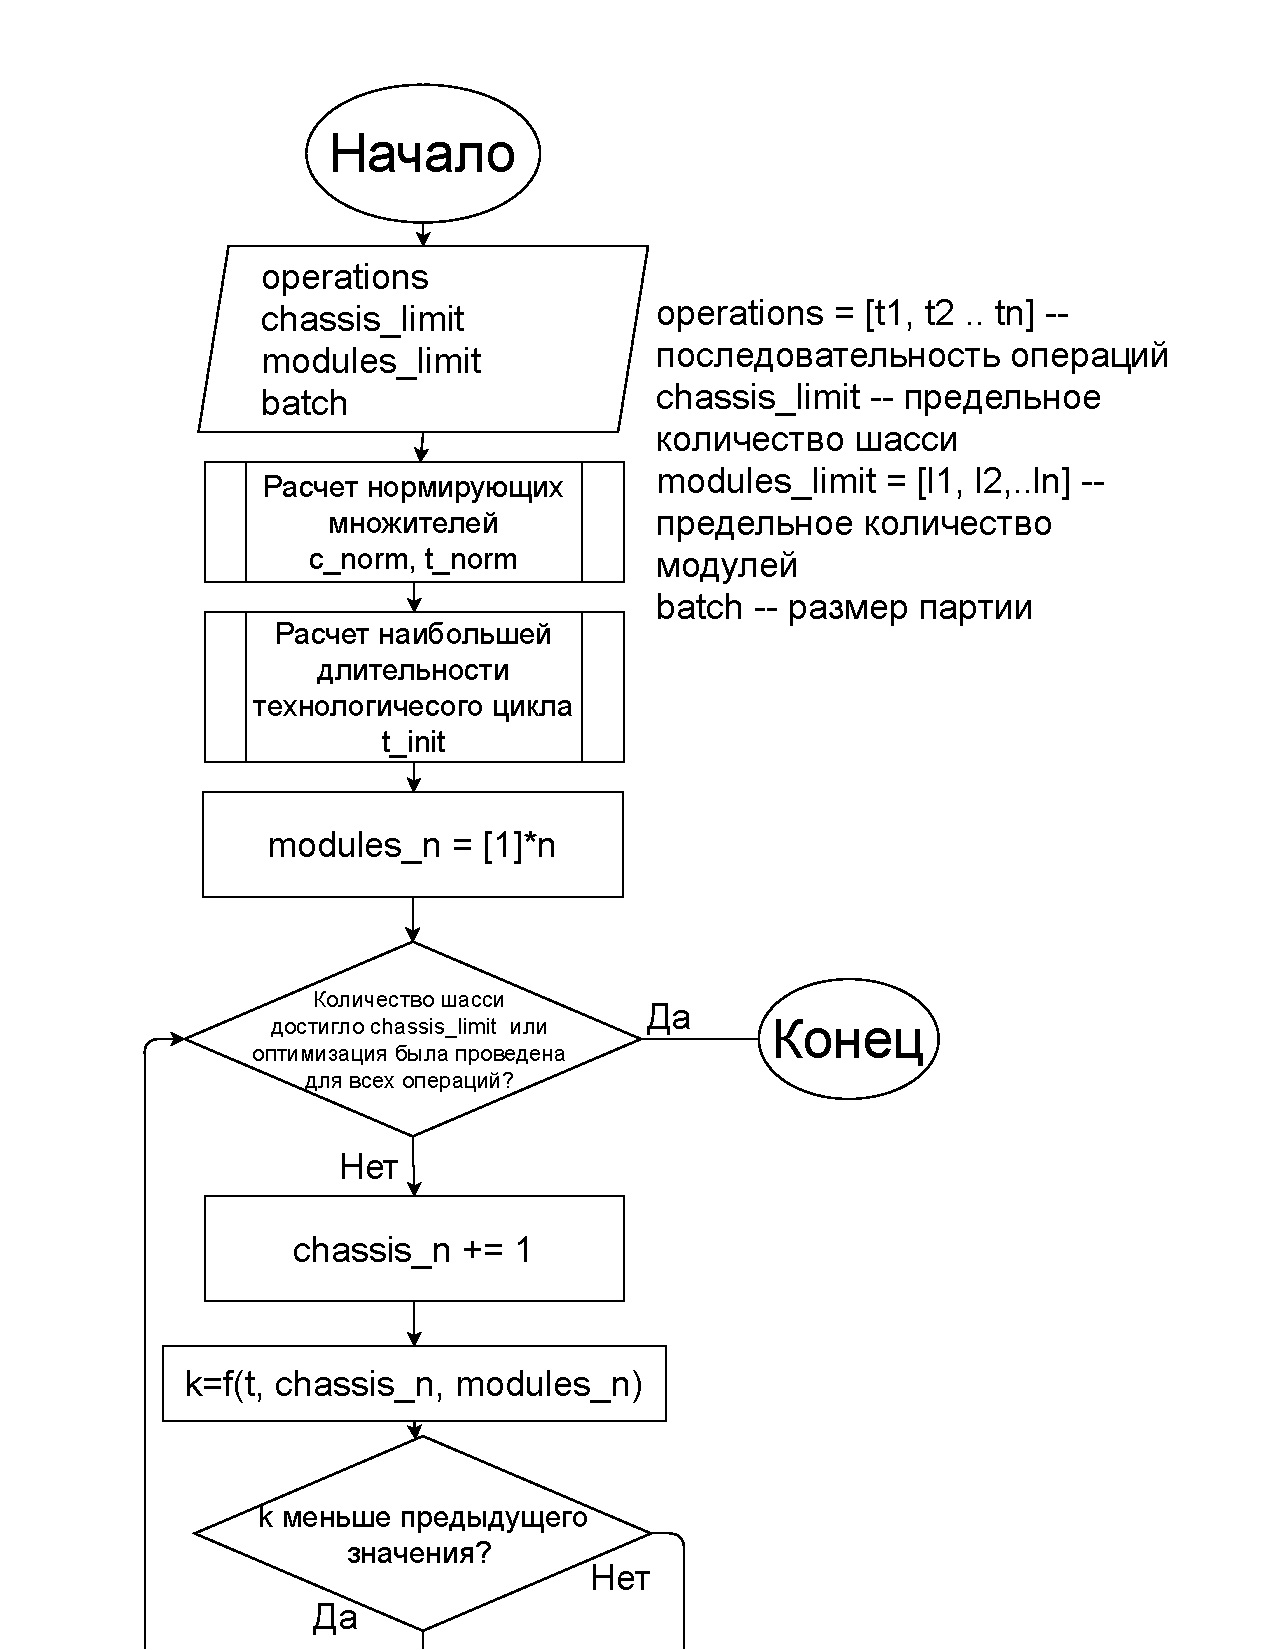
\includegraphics[width=\textwidth]{ch-2/algo-1}
	}
	\caption{Блок схема алгоритма оптимизации}\label{fig:algo-1}
\end{figure}


\paragraph{Первый этап.} На первом этапе производится расчёт нормирующих множителей. Значение нормирующего множителя \texttt{c\_norm} приравнивается  количеству видов модулей. То есть, если имеется 5 разных классов операций, выполняемых на модульном оборудовании, \texttt{то c\_norm = 5}. Затем необходимо определить нормирующий множитель технологического цикла \texttt{t\_norm}. Для этого производится расчёт длительности процесса для случая, когда \texttt{chassis\_n = c\_norm}, а \texttt{modules\_n} является единичным списком \texttt{[1, 1, 1...]}, длина которого совпадает с количеством классов модулей.  
 
\paragraph{Второй этап.} На этом этапе производится расчёт наихудшего варианта длительности \texttt{t\_init}.
Наихудший вариант может быть получен, когда имеется только одно шасси \texttt{chassis\_n = 1} и по одной единице модулей каждого вида \texttt{modules\_n = [1,1,1 ...]}. После чего для наихудшего варианта рассчитывается целевая функция \texttt{k\_prev = F(t, chassis\_n, modules\_n)}.

\paragraph{Третий этап.} Этот и дальнейшие шаги происходят в цикле. Цикл длится пока не будет превышен предел количества шасси или не будет проведен расчёт для каждой операции.

\begin{enumerate}
	\item Операции сортируются в порядки убывания длительности. При этом формируется список индексов операций. Затем значение индекса наиболее длительной операции сохраняется. Например, для \texttt{operations = [347.2, 1384.2, 437.7]} список индексов будет \texttt{indices[1, 2, 0]} и индекс наиболее длительной операции \texttt{ind = 1}.
	\item На этом шаге количество шасси инкрементируется  \texttt{chassis\_n += 1}. Рассчитывается длительность технологического  цикла \texttt{t}, после чего определяется значение  целевой функции \texttt{F(t, chassis\_n, modules\_n)}.
	\item Если результат целевой функции строго меньше предыдущего значения, то  текущее значение целевой функции сохраняется. Также сохраняются значения количества шасси и модулей, поскольку являются  оптимальными на данный момент. Переход обратно на шаг 1. В противном случае переход к шагу 4.
	\item Инкрементируется количество модулей, необходимых для операции с индексом \texttt{ind}. Это сопровождается расчётом целевой функции на каждой итерации. 
	\item Если значение целевой функции строго меньше предыдущего, то значения количества шасси и модулей сохраняются как оптимальные значения на данный момент, после чего переход к шагу 4. В противном случае происходит декремент индекса операции \mbox{\texttt{ind -= 1}} (предшествующая операция) и переход на шаг~4. Однако если операция первая, т.\,е. \texttt{ind - 1 < 0}, то сокращаем длительность операции в \texttt{min(chassis\_n, modules\_m[ind])} раз и переходим к шагу~1.
\end{enumerate}

Асимптотическая сложность для худшего случая полученного алгоритма $\mathcal{O}(n^2)$, против экспоненциальной сложности прямого перебора $\mathcal{O}(l^n)$, где $l$ "--- предельное количество модулей и шасси.
Для лучшего случая асимптотическая сложность будет $\mathcal{O}(n)$, в то время как прямой перебор все равно потребует проверки всех значений, т.\,е. его сложность будет $\mathcal{O}(l^n)$.


\subsection{Длительность технологического цикла}

Технологический цикл является частью производственного цикла, который представляет собой период от запуска детали (или партии деталей) в производство до получения готовой детали (или партии деталей). Длительность производственного цикла состоит из трех периодов:

\begin{itemize}
	\item Рабочее время.
		\subitem Технологический цикл.
		\subitem Время вспомогательных операций.
	\item Время естественных процессов, которые протекают без оказания воздействия на предмет труда человеком или оборудованием, но при этом происходит изменение состояния изделия.
	\item Время перерывов в работе, к ним относятся регламентированные и нерегламентированные перерывы. К нерегламентированным относятся перерывы обусловленные организационными и техническими причинами, например отказы оборудования.
\end{itemize}

Технологический цикл представляет собой период времени выполнения  всех основных технологических операций изготовления детали или суммой однооперационных циклов. Где однооперационный цикл "--- это время выполнения одной операции над партией деталей. Длительность технологического цикла может оказывать значительное влияние на весь производственный цикл в целом.~\footnote{Электронный ресурс: {\tiny\url{http://de.ifmo.ru/bk_netra/page.php?tutindex=3&index=107}} (дата обращения 12.12.2018).} Таким образом управление длительностью технологического цикла позволяют влиять на такие важные факторы производства как:

\begin{itemize}
	\item Производительность труда.
	\item Объёмы выпуска.
	\item Себестоимость окончательного изделия.
	\item Наличие незавершенного производства.
\end{itemize}

Перемещение предметов труда по технологическому циклу может происходит тремя способами:

\begin{itemize}
 	\item Последовательным.
	\item Параллельным.
    \item Последовательно-параллельным.
\end{itemize}

Последовательный цикл~(рисунок~\cref{fig:seq}) чаще всего используется на мелкосерийном и единичном производстве и представляет собой движение всей партии детали целиком -- от одной операции к другой. Переход на другую операцию осуществляется только в тот момент, когда на предыдущей обработаны все детали партии.
Его время вычисляется по формуле~\cref{eq:sc}:

\begin{figure}[!htb]
	\centerfloat{
		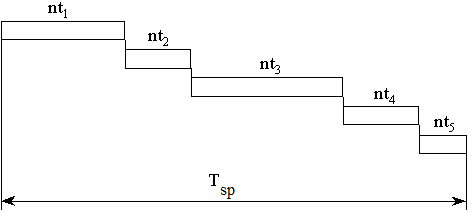
\includegraphics[width=0.5\textwidth]{ch-2/seq}
	}
	\caption{График последовательного вида движения}\label{fig:seq}
\end{figure}

\begin{equation}
T_{sc} = n t_{1} + n t_{2} + \ldots + n t_{K_0} = n \sum_{j=1}^{K_{0}}t_{j},
\label{eq:sc}
\end{equation}


\noindent где: $n$ "--- количество изделий в партии, $K_{0}$ "--- число операций обработки в соответствии с технологическим процессом,  $t_{j}$ "--- штучно-калькуляционное (операционное) время на $j$-ю операцию.

В отличии от последовательного движения при параллельное движении~(рисунок~\cref{fig:parallel}) передача детали от операции к операции происходит поштучно или транспортными партиями, на которые разбивается основная. Зачастую используется в серийном и массовом производстве, однако возможно применение и в мелкосерийном.

Длительность в таком случае рассчитывается по формуле~\cref{eq:pc}:

\begin{figure}[!htb]
	\centerfloat{
		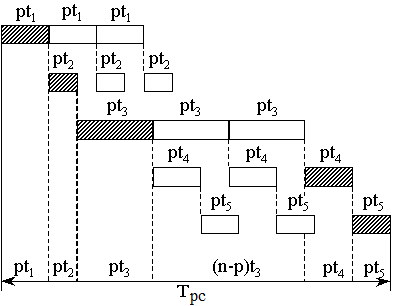
\includegraphics[width=0.5\textwidth]{ch-2/parallel}
	}
	\caption{График параллельного вида движения}\label{fig:parallel}
\end{figure}

\begin{equation}
T_{pc} = p\sum_{j=1}^{K_{0}}t_{j}+(n-p)t_{main},
\label{eq:pc}
\end{equation}

\noindent где: $p$ "--- размер транспортной партии, кратный целой партии $n$, $t_{main}$ "--- время главной операции.

Параллельно-последовательный вид движения~(рисунок~\cref{fig:seq-parallel}) представляет собой сочетание двух предыдущих походов~\cref{eq:spc}. Передача детали осуществляется поштучно или транспортными партиями. При этом начало обработки на следующей операции происходит со смещением, таким образом, чтобы избавиться от микропауз, возникающих в последовательном типе движения . Однако применяется по большей части только при массовом и крупносерийном производстве, поскольку требует налаженного ритма производства.

\begin{figure}[!htb]
	\centerfloat{
		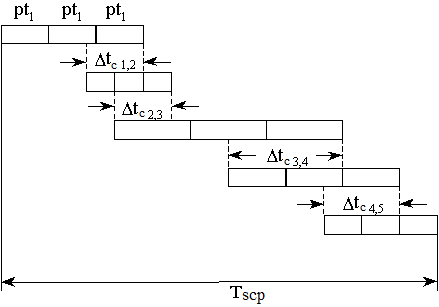
\includegraphics[width=0.5\textwidth]{ch-2/seq-parallel}
	}
	\caption{График параллельно-последовательного вида движения}\label{fig:seq-parallel}
\end{figure}

\begin{equation}
T_{spc} = T_{sc} - \sum_{j=1}^{K_{0}-1}\Delta t_{c \;  j,j+1} = n \sum_{j=1}^{K_0}t_j-(n-p)\sum_{j=1}^{K_{0}-1}t_{short \; j,j+1},
\label{eq:spc}
\end{equation}

\noindent где: $\Delta t$ "--- разность времени пары смежных операций, $t_{short}$ "--- время кратчайшей из пары смежных операций. 

Для расчета критерия оптимизации на каждой итерации требуется определение длительности технологического цикла. Вместе с этим применение концепции модульного оборудование позволяет не просто применять последовательный вид движения, но и использовать транспортные партии попеременного размера. Это обуславливается тем фактом, что часть технологического оборудования можно реконфигурировать в процессе технологического цикла, повышая или понижая производительность того или иного однооперационного цикла.  Это в свою очередь позволяет уменьшить длительность технологического цикла в сравнении с немодульным оборудованием.

\subsection{Проведение вычислительного эксперимента}

Для проверки корректности целевой функции и предложенного алгоритма оптимизации был проведен оптимизационный эксперимент на основе симуляции в программном обеспечении Anylogic. В данной системе была построена диаграмма процесса производства печатной платы изделия <<Гироподвес>>.

Для построения использовался дискретно-событийный метод,\footnote{Электронный ресурс: {\tiny\url{anylogic.ru/use-of-simulation/discrete-event-simulation}} (дата обращения: 13.12.2019).} представляющий движение предмета труда от одной технологической операции к другой в виде задержек на период длительности операции. Для определения длительности технологических переходов операций, выполняемых на станках ЧПУ, была проведена симуляция в CAM-системах CAMotics и Fusion 360 (см. приложение). Длительность вспомогательных переходов определялась в соответствии с общемашиностроительными нормативами времени для нормирования работ, выполняемых на универсальных и многоцелевых станках с числовым программным управлением.\footnote{Электронный ресурс: \url{standartgost.ru/g/pkey-14293832230} (дата обращения: 14.02.2020).} При этом в технологическом процессе присутствуют операции, выполнение которых происходит без применения технологического оборудования с ЧПУ. Сюда относятся операции нанесения фоторезиста, травление и проявка, длительность которых определялась в соответствии с ОСТ 107.460092.004.01-86\footnote{ОСТ 107.460092.004.01-86. Платы печатные. Типовые технологические процессы. Часть первая.} и документации на фоторезист. Длительность всех технологических операций представлена в маршрутной карте (приложение~\cref{app:A}).

Технологические операции, выполняемые на основе оборудования с ЧПУ, могут быть выполнены с применением модульного оборудования. В таблице~\cref{tab:cnc-modules} представлено соответствие классов технологических операций и модулей.

\begin{table} [!htb]
	\centering
	\caption{Соответствие классов операций, рассматриваемого технологического процесса, и технологических модулей} \vspace{4pt}
	\label{tab:cnc-modules}
	\begin{threeparttable}
		\begin{tabularx}{\linewidth}{ll}
			\toprule
			\textbf{Код операции\tnote{1}} & \textbf{Наименование модуля} \\
			\midrule
			4232 & Сверлильный модуль \\
			5541 & Лазерный модуль \\
			4234 & Фрезерный модуль \\
			\bottomrule
		\end{tabularx}
		\begin{tablenotes} \footnotesize
			\item [1] Код из классификатора операций 1 85 151.
		\end{tablenotes}
	\end{threeparttable}
\end{table}

Построение оптимизационного эксперимента начинается с определения варьируемых параметров, их предельных значений и шага.  Также в симуляцию добавлен параметр, определяющий размер партии, однако в процессе оптимизации он является фиксируемым. Значение параметров, используемых в симуляции представлены в таблице~\cref{tab:par-anylogic}.

\begin{table} [!htb]
	\centering
	\caption{Параметры оптимизационного эксперимента в системе Anylogic} \vspace{4pt}
	\label{tab:par-anylogic}
	\begin{threeparttable}
		\begin{tabularx}{\linewidth}{lllll}
			\toprule
			Параметр & Вид параметра & Мин. & Макс. & Шаг \\
			\midrule
			Количество шасси               & дискретный  & 1 & 10 & 1 \\
			Количество сверлильных модулей & дискретный  & 1 & 10 & 1 \\
			Количество лазерных модулей    & дискретный  & 1 & 10 & 1 \\
			Количество фрезерных модулей   & дискретный  & 1 & 10 & 1 \\
			Размер партии                  & фиксируемый & 3 &  - & - \\
			\bottomrule
		\end{tabularx}
	\end{threeparttable}
\end{table}

Следующим этапом указывается целевая функция~\cref{eq-2-22}, предложенная в разделе~\cref{sec:target-func}. При этом необходимо указать весовые коэффициенты и нормирующие коэффициенты. Для данного технологического процесса были рассчитаны весовые коэффициенты в соответствии с разделом~\cref{sec:weight}. 
Нормирующие коэффициенты были определены при проведении симуляции с параметрами количества шасси, эквивалентному применению минимально возможному количеству немодульного оборудования с ЧПУ. Одна единица немодульного оборудования считается эквивалентной сочетанию одного шасси и одного модуля.

После проведенных подготовительных расчётов, автоматически генерируется графический интерфейс и запускается оптимизация. В Anylogic оптимизация происходит по алгоритму прямого перебора незафиксированных параметров. Результаты симуляции представлены в таблице~\cref{tab:res-anylogic}, а внешний вид окна эксперимента на рисунке~\cref{fig:win-anylogic}.

\begin{table} [!htb]
	\centering
	\caption{Результаты оптимизации технологического цикла производства изделия <<Гироподвес>> с применением модульного оборудования в системе Anylogic} \vspace{4pt}
	\label{tab:res-anylogic}
	\begin{threeparttable}
		\begin{tabularx}{\linewidth}{ll}
			\toprule
			Параметр & Значение \\
			\midrule
			Количество шасси               & 2\:ед. \\
			Количество сверлильных модулей & 2\:ед. \\
			Количество лазерных модулей    & 1\:ед. \\
			Количество фрезерных модулей   & 1\:ед. \\
			Длительность цикла             & 3,5 ч. \\
			Количество итераций            & 112 \\
			\bottomrule
		\end{tabularx}
	\end{threeparttable}
\end{table}

\begin{figure}[!htb]
	\centerfloat{
		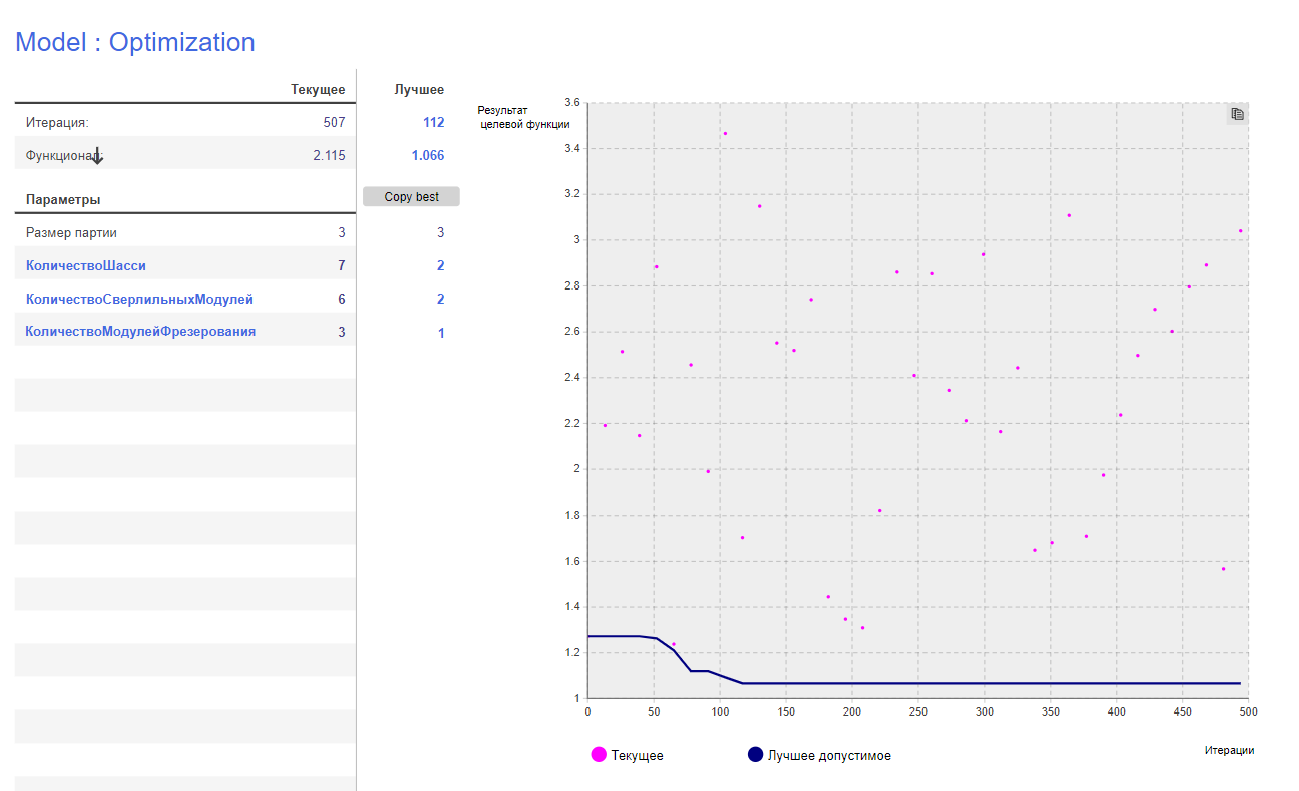
\includegraphics[width=\textwidth]{ch-2/win-anylogic}
	}
	\caption{Внешний вид окна эксперимента в среде Anylogic}\label{fig:win-anylogic}
\end{figure}


Для проверки предложенного алгоритма оптимизации была написана программа на языке  Python версии 3.8. Результаты представлены в таблице~\cref{tab:res-python}.
Результаты оптимизации совпали с результатами в системе Anylogic (см. таблица~\cref{tab:res-anylogic}). Что позволяет судить о корректности алгоритма оптимизации.

\begin{table} [!htb]
	\centering
	\caption{Результаты оптимизации на основе предложенного алгоритма\\на языке Python} \vspace{4pt}
	\label{tab:res-python}
	\begin{threeparttable}
		\begin{tabularx}{\linewidth}{ll}
			\toprule
			Параметр & Значение \\
			\midrule
			Количество шасси               & 2\:ед. \\
			Количество сверлильных модулей & 2\:ед. \\
			Количество лазерных модулей    & 1\:ед. \\
			Количество фрезерных модулей   & 1\:ед. \\
			Длительность цикла             & 3,5 ч. \\
			Количество итераций            & 21 \\
			\bottomrule
		\end{tabularx}
	\end{threeparttable}
\end{table}

Максимально близким эквивалентным комплектом немодульного оборудования является конфигурация указанная в таблице~\cref{tab:equal}, при этом  для данного комплекса была также получена длительность технологического цикла.

\begin{table} [!htb]
	\centering
	\caption{Состав эквивалентного комплекта немодульного оборудования} \vspace{4pt}
	\label{tab:equal}
	\begin{threeparttable}
		\begin{tabularx}{\linewidth}{ll}
			\toprule
			Тип немодульного оборудования & Количество, ед. \\
			\midrule
			Сверлильный станок c ЧПУ & 1 \\
			Установка LDI            & 1 \\
			Фрезерный станок с ЧПУ   & 1 \\
			\bottomrule
		\end{tabularx}
	\end{threeparttable}
\end{table}


Для данного комплекта также была рассчитана длительность технологического цикла, которая составила 4,27\:ч., что на \textit{18\:\% больше}, чем при использовании комплекта модульного оборудования.


%-----------------------------------------------------------------------------------------------------------------------------------------------

%\section{Математическая модель унификации, параметризации и оптимизации компонентов модульной технологической платформы}
%
%\section{Модель оптимизации модульного оборудования при единичном и мелкосерийном производствах}

%Рассмотрим основные понятия оптимизации по номенклатуре выпускаемых изделий. Пусть $N$ "--- номенклатура групп изделий, предлагаемая для выпуска, полученная на этапе маркетинговых исследований:



%\noindent где $D_i$ "--- группа изделий. Группирование происходит по технологическому признаку [Митрофанов, стр. 43] "--- \textit{вид обработки}.
%
%
%
%\noindent где $P_j$ "--- групповая технологическая операция. В соответствие каждой группе ставится вероятность спроса:
%
%\begin{equation}
%f: D_i \rightarrow \upsilon_i, D_i \in N, \upsilon_i \in V,
%\end{equation}
%
%\noindent где $V$ "--- множество вероятностей такое, что:
%
%\begin{equation}
%\forall\upsilon\in V: \upsilon\leq 1 \wedge\upsilon > 0
%\end{equation}
%
%Определим композицию для нахождения наиболее вероятной группы или нескольких групп:
%
%\begin{equation}
%g: V \rightarrow N', \forall\upsilon = V_max: \upsilon \in f(N'), V_max \in V, N' \subset N
%f \ g = h,
%\end{equation}
%
%\noindent где $N' = (D_j)_{j \in J}$ "--- результат композиции (семейство наиболее вероятных групп), $\bigcup N' = {p:p_1\in D_1 \vee p_2\in D_2 \vee\ldots\vee p_j\in D_j}$ "--- множество групповых операций в этих группах.
%
%Фактическая номенклатура задаётся нечётким множеством:
%
%\begin{equation}
%N'' = {(D, \upsilon(D)) \mid D \in N}
%\end{equation}
%
%Определить коэффициенты целесообразности использования модульности можно как:
%
%\begin{equation}
%\epsilon = \frac{\big|\bigcup N' \big|}{|G|},
%\end{equation}
%
%\noindent где $G$ "--- домен операций, $\bigcup\limits_{i} N$. Если $\epsilon\rightarrow 0$ "--- модульность целесообразна, если $\epsilon\rightarrow 1$ "--- модульность нецелесообразна.

%\section{Определение критерия оптимизации конфигурации модульного оборудования}
%
%\section{Разработка параметрического ряда ширины присоединительной поверхности}

\section{Выводы по главе 2}

В настоящей главе было проведено исследование методик проектирования и применения модульного оборудования. Были рассмотрены подходы к унификации оборудования, а также существующие стандарты унификации. На основании проведённого анализа можно сделать вывод о том, что на сегодняшний день не существует единого подхода к унификации и стандартизации модульного оборудования, однако отдельные стандарты унификации существуют. Именно на их основании можно проводить унификацию модульного оборудования. 

Далее рассматриваются особенности проектирования модулей. Отмечается, что на модули в первую очередь должны быть наложены ограничения, связанные с удобным и быстрым креплением модулей. Поэтому основное внимание нужно уделить конструкции сопрягаемых поверхностей и способу крепления. На основании сформулированных требований к устройству крепления модулей предлагается система быстрой установки модулей, основанная на применении специальной формы сопрягаемых поверхностей с направляющим пазом и элекромагнитом.

На основании предложенной конструкции системы крепления выбирается ряд параметров модуля, из которых выбирается главный параметр, также задаются фиксированные параметры. Главным параметром выбрана грузоподъемность электромагнита. В качестве основных параметров выбраны: ширина присоединительной поверхности модуля, глубина модуля, ширина модуля, ток потребления модуля. В качестве фиксированных параметров приняты напряжение питания, геметрические параметры ответной части паза крепления. Для модулей с электромагнитным креплением было выявлено пять ограничений: ограничение массы модуля в зависимости от грузоподъемности электромагнита, ограничение грузоподъемности электромагнита в зависимости грузоподъемности шасси, ограничение тока потребления модуля в зависимости от максимального рабочего тока шасси, ограничение глубины модуля в зависимости от размера рабочего пространства, ограничение на ширину присоединительной поверхности модуля. На основании параметров и ограничений предложены основные кратные ряды для модулей.

Следующим пунктом предложена методика расчёта показателя целесообразности применения модульного оборудования. В качестве аналога показателя целесообразности рассматривается метрика общей эффективности оборудования, модифицированная для случай применения модульного оборудования в мелкосерийном и единичном производстве. Показатель целесообразности позволяет оценить перспективы использования модульного оборудования для типовых технологических процессов, используемых на предприятии. Для проверки правильности данного критерия, был разработан технологический процесс изготовления изделия <<гироподвес>>, после чего проведен расчёт критерия целесообразности, который показал, что для данного технологического процесса с заданным годовым объёмом выпуска, использование модульного технологического оборудования целесообразно. Данный результат позволил прийти к выводу о том, что применение предложенного критерия может выступать в качестве приближенной оценки, позволяющий с минимальными затратами вычислительных ресурсов определить необходимость в дальнейших расчётах. Для проверки правильности данной гипотезы, была проведен ряд вычислительных экспериментов в среде дискретно-событийного моделирования AnyLogic, который показал, что при использовании модульного оборудования для данного технологического процесса прирост производительности составляет~\SI{18}{\percent} из чего был сделан вывод о том, что математическое описание критерия целесообразности было определено верно.

Следующим этапом исследования вопросов повышения эффективности применения модульного оборудования стала разработка методики оптимизации комплекта модульного оборудования, то есть определения наиболее оптимального состава модулей и шасси для конкретного технологического процесса. Первоначально были определены частные критерии оптимизации. Для комплекта модульного технологического оборудования было выделено два критерия "--- стоимость предлагаемого комплекта оборудования и длительность технологического цикла. С помощью метода аддитивной свертки был произведён переход от двухкритериальной оптимизации к однокритериальной. Была описана целевая функция и произведён расчёт весовых коэффициентов. Суть алгоритма оптимизации заключается в итерации от главной операции (зачастую являющейся узким местом)  к менее главным, сопровождающейся добавлением шасси и модулей, а затем оценкой значения целевой функции. Главной операцией считается операция с наибольшей длительностью. 

\FloatBarrier           % Глава 2
\chapter{Информационное взаимодействие компонентов модульного технологического оборудования}\label{ch:ch3}

\section{Подсистема управления модульным оборудованием}\label{sec:ch3/sec1}

Современные системы управления технологическим оборудованием сложны и надежны. Каждый их элемент представляет собой черный ящик с жесткой иерархической архитектурой. Все в таких системах ориентировано на обеспечение качества, надежности и отказоустойчивости. Инерция таких систем вынуждает разработчиков использовать монолитную архитектуру, поскольку оборудование с распределенным управлением не может быть легко добавлено в распределенную производственную среду.

Следовательно, акцент делается на концепции интеграции. Другими словами, разработчики сосредоточились на объединении разнородных компонентов в одну производственную систему вместо использования концепции взаимодействия. Концепция взаимодействия влечет за собой создание открытого интерфейса, который позволяет компонентам оставаться в автономном состоянии с возможностью обмена данными.

Рассматриваемое модульное оборудование требует переосмысления данного подхода и создания системы управления, которая состоит из взаимозаменяемых строительных блоков с описанной унификацией ввода и вывода. При создании новой конфигурации оборудования (установке модуля/модулей на шасси) должна автоматически изменяться и подсистема управления получившимся оборудованием. Следовательно устройство ЧПУ должно знать о каждом возможном модуле заранее, то есть снова будет получена монолитная система с иерархическим управлением.

Следовательно, необходимо выделить основную часть архитектуры и определить спецификации в отношении протокола связи, а также правила создания новых программных и аппаратных модулей, которые могут быть динамически подключены к системе. Впоследствии в основную часть войдет алгоритм управления двигателями координатного шасси, а остальная часть будет внешними компонентами.

Такой подход дает возможность полностью изменить парадигму среды управления производством. К сожалению, не все так просто. Система ЧПУ - это не только алгоритм управления, но и база данных, пользовательский интерфейс и компонент связи с физической средой (также известный как <<встроенные системы>> и <<микроконтроллеры>>). Для реализации такой системы требуется системный подход, поэтому предлагается использовать шаблон архитектуры микросервисов~\cite{microservices2017indin}.

\section{Сетевая архитектура модульного оборудования}\label{sec:ch3/sec2}

Основная особенность модульного промышленного оборудования заключается в возможности быстрой переналадки любой единицы оборудования при смене технологического процесса. Переналадка осуществляется за счет смены обрабатывающих головок и внешних модулей.  Это достигается посредством максимальной автономности каждого модуля. Все они обладают собственными алгоритмами функционирования, а также набором датчиков и исполнительных устройств. Все модули могут общаться друг с другом по единому протоколу, при этом набор команд и данных сведен к минимуму, все команды строго регламентированы.

Основным модулем является многокоординатное шасси, которое осуществляет перемещение обрабатывающих головок в пространстве. Естественно, с точки зрения управления такая система не может быть полностью децентрализованной "--- с каждой единицей оборудования связана ее виртуальная диспетчер (<<цифровой двойник>>), который является моделью оборудования и осуществляет координацию модулей, головок и шасси. Именно наличие диспетчера позволяет осуществить быструю переналадку оборудования. Все модули настроены одинаково, все они знают свои возможности и протокол взаимодействия, поэтому при физическом подключении находят в сети своего диспетчера, регистрируют свои сервисы, после чего сразу готовы к работе.

Данная концепция отлично работает, если представить, что у нас есть только одна единица оборудования, однако это не так. Индустриальная кибер-физическая система (сокр. \textit{ИКФС}) может состоять из многих сотен и тысяч устройств, причем подавляющее большинство этих устройств является именно технологическим оборудованием. При этом, как уже было сказано выше, каждая единица оборудования, каждый модуль и каждый датчик подключены к единой децентрализованной mesh-сети, т.\:к. являются частями одной ИКФС.

Здесь сразу прослеживается проблема: если все модули находятся к децентрализованной сети и имеют возможность найти своего диспетчера, то как они могут определить, что именно этот диспетчер физически подключен к данному модулю. Естественное решение: возложить эту обязанность на оператора. Однако это сломает принцип zero config, то есть оператор должен думать только о технологическом процессе, а не о конфигурации/переконфигурации оборудования. Здесь можно привести аналогию с обычным универсальным оборудованием. Рабочий, производящий операции, например, на токарном станке, не должен задумываться об информационной совместимости инструмента и станка. Ему достаточно физической совместимости. Например, резец физически помещается в резцедержатель. Именно подобной простоты переналадки мы и хотим добиться в своей работе, только не для <<глупого>> универсального оборудования, а для <<умного>>, интегрированного в ИКФС.

Из всего вышесказанного можно сделать вывод о том, что организация ячеистой сети ИКФС, в которой используется модульное оборудование, не является тривиальной задачей. Поэтому оставшаяся часть раздела будет посвящена вопросам развертывания тестовой сети OpenThread, описанию общей архитектуры ИКФС, построенное на ее основе, а также принципов работы модульного оборудования, входящего в ИКФС.

Как уже было отмечено в предыдущем разделе по совокупности достоинств и недостатков в качестве опорной сети ИКФС была выбрана технология OpenThread. Данный протокол беспроводной передачи данных является реализацией сетевого протокола Thread изначально разработанного компанией Google Nest. Отличительной особенностью OpenThread является максимальная переносимость, при этом в соответствии со спецификацией  могут быть реализованы различные designs, как чисто аппаратные, так и программно-аппаратные. Подобная гибкость позволяет сначала создать структуру опорной сети с применением технологий виртуализации, протестировать и отладить ее, а затем перенести на физические устройства.

Для развертывания виртуальной сети был использован набор отладки, находящийся в репозитории OpenThread. В частности, 	использовалась сборка сетевого клиента под архитектуру x86 с эмуляцией радиомодуля посредством сетевой карты с передачей сообщений по протоколу UDP. Первостепенными задачами стали построение простейшей сети и отработка на ее примере алгоритма взаимодействия узлов. В целях упрощения задачи первоначальная структура сети состояла из трех независимых узлов. Каждый узел сети развертывается единообразно, что позволило автоматизировать этот процесс в виртуальном окружении.
В соответствие со спецификацией протокола существует два вида узлов: 

\begin{enumerate}
	\item Router, который никогда не выключает приемопередатчик, участвует в передаче пакетов по сети, а также является узлом обеспечения безопасности для всех вновь подключающихся устройств.
	\item End Device, который преимущественно взаимодействует только со своим роутером, не осуществляет передачу данных по сети и может выключать свой приемопередатчик для экономии энергии.
\end{enumerate}

Из всего множества Routers один (как правило, включившийся первым) назначается Leader. Leader агрегирует и распространяет информацию о конфигурации всей сети, в одной PAN (Personal Area Network) может быть только один лидер.  В целях обеспечения надежности и отказоустойчивости роль лидера динамически переходит от одного узла к другому, то есть любой роутер может self-elect в качестве лидера. Также в сети может быть назначен один Border Router, отвечающий за взаимодействие и передачу IPv6 трафика между mesh-сетью OpenThread и другими сетями, например, Wi-Fi.

Таким образом, тестовая сеть будет состоять из одного Router, с назначенной ролью Leader и двух Router Eligible End Devices, которые позволят продемонстрировать возможность изменения роли при отключении/подключении узлов.

После старта первый узел проверяет сеть на наличие других узлов и, так как других узлов в сети нет, назначает себе роль Router и Leader. Второй и третий узлы настраиваются с помощью тех же команд. Единственное отличие: в процессе первоначального сканирования сети узлы видят, что в сети уже есть один Router, поэтому первоначально присваивают себе роль Child, которая автоматически меняется на Router после двухминутного таймаута. Это связано с тем, что сеть Thread старается поддерживать количество Routers в сети в диапазоне 16--23, соответственно до достижения минимального значения каждый вновь подключенный узел будет менять свою роль на Router.

Продемонстрированный пример конфигурации тестовой сети OpenThread наглядно показывает, что можно осуществлять полную предварительную настройку устройств без необходимости ручного подключения нового устройства к сети. При этом можно отметить, что настройка является очень простой процедурой, подключение к сети происходит очень быстро, и после старта любой узел сети сразу видит все соседние узлы и может осуществлять взаимодействие с ними по протоколу IPv6.

\subsection{Протокол взаимодействия}

В предыдущем разделе была рассмотрена процедура физического развертывания децентрализованной backbone сети ИКФС. Результатом является готовая опорная  (backbone) сеть, в которой узлы могут обмениваться сырыми данными. Однако нельзя забывать, что данная система не является обычной сенсорной сетью, где используются только простейшие протоколы прикладного уровня, например, очередь сообщений MQTT.

Безусловно, наличие всевозможных датчиков мониторящих производственный процесс подразумевается, но основа ИКФС "--- это модульное промышленное оборудование. С одной стороны оно состоит из автономных и независимых модулей, находящихся в общей mesh-сети. С другой "--- все эти модули способны организовывать устойчивые иерархические формации для выполнения конкретных задач производства. Из последнего утверждения следует, что для эффективной работы подобной гетерогенной сети нужен более сложный протокол для двустороннего взаимодействия.

Рассмотрим данный протокол более подробно. Консолидация модулей осуществляется вокруг базового модуля, выполняющего роль диспетчера. Так как предполагается, что для обеспечения гибкости оборудования, оно должно быть максимально унифицировано, каждая единица оборудования включает в свой состав обязательный модуль "--- трехкоординатное шасси, осуществляющее перемещение обрабатывающих головок в пространстве. Безусловно, многие виды обработки требуют возможности перемещения рабочего органа по 4 или 5 координатам, но, как показывает практика, во многих даже профессиональных 5-координатных обрабатывающих центрах в качестве основы используется именно трехкоординатное шасси, а дополнительные координаты выполнены в виде отдельного модуля. Соответственно, с точки зрения управления, именно трехкоординатное шасси выполняет роль диспетчера, вокруг которого конфигурируется та или иная единица оборудования. 

Каждый диспетчер имеет реестр, представляющий собой часть распределенного JSON-based хранилища. Реестр состоит из слотов, в каждом из которых может быть зарегистрирован один модуль. В свою очередь, совокупность всех реестров представляет собой цифровую модуль ИКФС и хранится в облаке. Для единообразия по той же схеме создается цифровая модель устройств, не являющихся промышленным оборудованием (в первую очередь это различные датчики производственного процесса). Датчик является диспетчером с одним слотом без возможности перерегистрации.

\begin{figure}[ht]
	\centerfloat{
		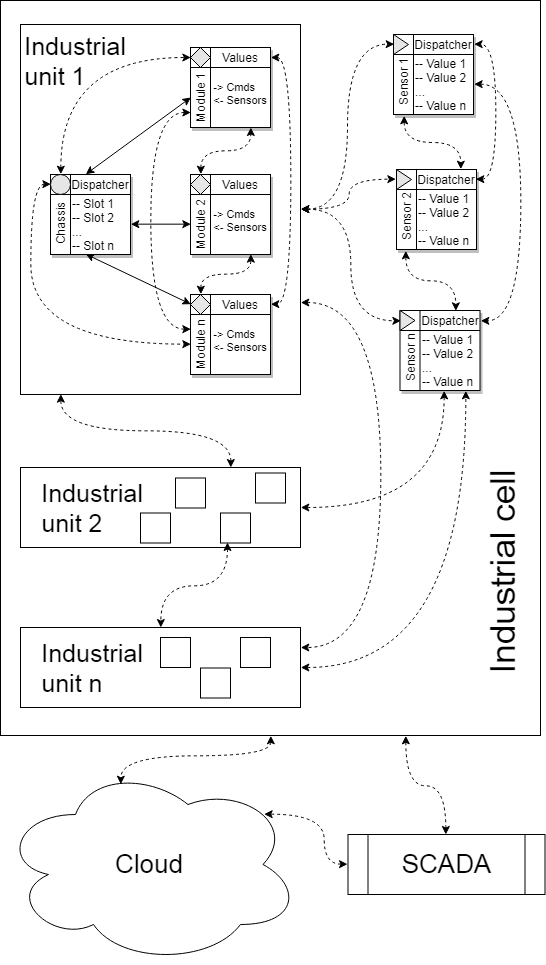
\includegraphics[width=0.5\textwidth]{ch-3/main-arch}
	}
	\caption{Слотовая модель модульного оборудования}\label{fig:main-arch}
\end{figure}

Слот "--- это запись типа <<ключ-значение>>, из которой диспетчер извлекает необходимые данные. Слот включает в себя следующие поля:

\begin{enumerate}
	\item адрес;
	\item название модуля/датчика;
	\item функции;
	\item возвращаемое значение;
	\item пределы возвращаемого значения.
\end{enumerate}

В качестве адреса выступают IPv6-адрес и порт, необходимые для взаимодействия с модулем. Название должно быть представлено в строковом виде или числовым идентификатором. Доступные для выполнения функции описываются набором G-кодов и М-функций в соответствии со стандартами ISO 6983-1 и ISO/TR 6983-2.
Например, фрезерный модуль будет представлять возможность работать с командами M3 и M4 (запуск шпинделя по и против часовой стрелки CW/CCW), M5 (останов шпинделя) и S (скорость вращения); для лазерного модуля "--- это будут команды M3 (включить лазер), М5 (выключить) и S (задать мощность в процентах); для магазина инструментов "--- M6 (сменить инструмент) и T (выбрать инструмент из магазина по номеру).  При этом все команды, связанные с перемещением модуля в трех основных координатах определяются модулем координатного шасси.

\begin{figure}[ht]
\centerfloat{
	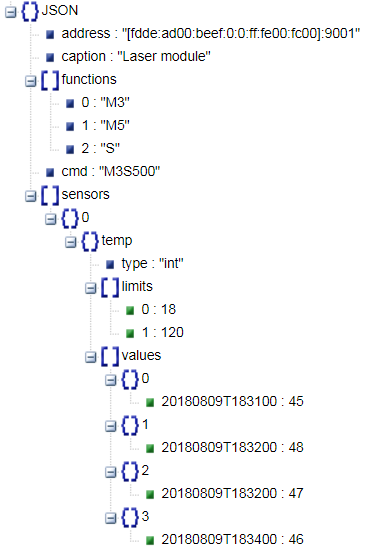
\includegraphics[width=0.5\textwidth]{ch-3/json}
}
\caption{Иерархическая структура единого реестра в формате JSON}\label{fig:json}
\end{figure}

Возвращаемое значение не обязательно должно быть одним. Описание каждого из них включает в себя тип, пределы и массив значений с временными метками. Диспетчер контролирует выход каждого значения за допустимые пределы, и в случае возникновения такой ситуации – осуществляет анализ возникшей ошибки, и принимается решение о возможности или невозможности продолжения работы оборудования.

Рассмотрим теперь процедуру регистрации модуля в реестре диспетчера. С точки зрения протокола "--- здесь нет никаких проблем: просто передача бинарного JSON-сообщения через очередь сообщений с последующей записью в распределенное хранилище. Однако не стоит забывать, что все диспетчеры и все модули находятся в единой самоорганизующейся mesh-сети. Возникает вопрос "--- как модуль определит к какому конкретно диспетчеру он подключен физически.

Предлагается следующее решение. Физическое подключение каждого модуля реализуется по трехпроводному интерфейсу, где по двум проводникам передается питающее напряжении, а третий используется в качестве линии безопасности (safety line). Линия безопасности объединяет все модули одной единицы оборудования по схеме монтажное И. В данной схеме линия безопасности подтянута резистором к плюсу питания. Так как сопротивление между линией и землей бесконечность, а между питанием и линией равно номиналу резистора, то напряжение на линии равно напряжению питания. То есть высокий уровень или логическая единица. Все модули подключены к линии и могут замыкать её на землю. Соответственно, на линии будет высокий уровень только тогда, когда все модули выставят высокий уровень на своих выходах. Как только любой из модулей соединит линию с землей, на ней установится низкий логический уровень и не один модуль не сможет на это повлиять.

\begin{figure}[ht]
\centerfloat{
	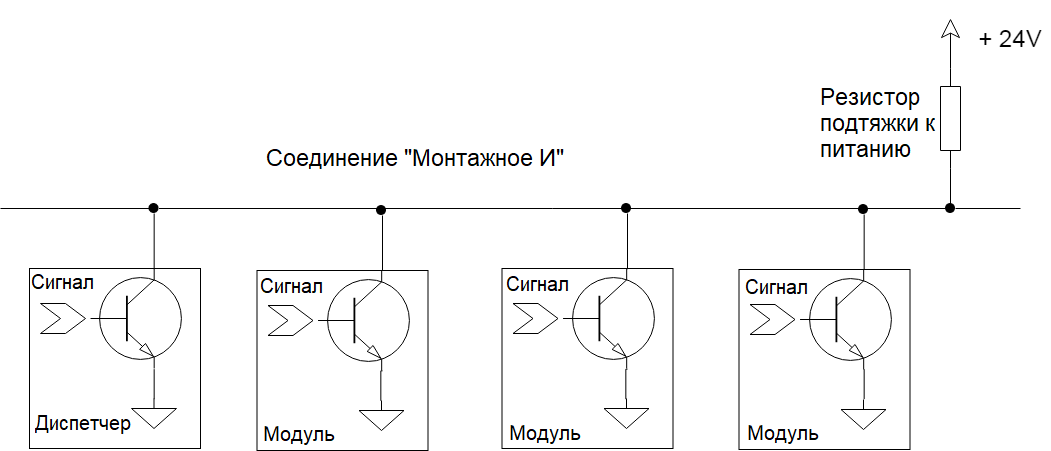
\includegraphics[width=\textwidth]{ch-3/logic-and}
}
\caption{Схема шины безопасности}\label{fig:logic-and}
\end{figure}

Таким образом, основная задача линии безопасности "--- регистрировать аварийные ситуации. В случае возникновения аварии в любом из модулей, он просто соединяет линию безопасности с землей, что является сигналом для других модулей прекратить работу и перейти в режим восстановления после сбоя. Необходимо отметить, что к этой же линии подключена являющаяся обязательной для любого промышленного оборудования кнопка аварийного останова, а также все двери безопасности, если они предусмотрены конструкцией.

Однако в процессе инициализации модулей линия безопасности может быть использована для регистрации новых модулей. Вновь подключенный модуль вначале осуществляет подключение к сети OpenThread, затем переводит линию безопасности на низкий логический уровень. Диспетчер детектирует это, после чего получает список всех ближайших к нему узлов (neighbors в терминологии OpenThread), выбирает среди них те, которые имеют статус не подключен, после чего просит первого из них перевести линию обратно на высокий логический уровень. Если уровень изменился, значит диспетчер и модуль подключены к одной линии, следовательно, модуль может быть зарегистрирован в реестре. В противном случае, диспетчер переходит к следующему модулю в списке.

\subsection{Методика определения максимальной пропускной способности канала передачи данных}

Так как основой предлагаемой сетевой архитектуры является открытый интерфейс, который позволяет аппаратным компонентам оставаться автономными, но в то же время при необходимости обмениваться данными с другими компонентами. Очевидно, что создать такой интерфейс без унификации протокола передачи данных невозможно. Этот протокол должен работать, прежде всего, со всеми протоколами и обеспечивать возможность прозрачного обмена информацией между процессами операционной системы, а также между узлами разнородной сети, которые могут действовать как программная служба, работающая под управлением операционной системы и физического контроллера.

Всем этим требованиям удовлетворяют уже упомянутые очереди сообщений. Очередь сообщений "--- это протокол асинхронной связи, поэтому получатель и отправитель не взаимодействуют напрямую, а вместо этого используют очередь сообщений. Очереди сообщений повышают отказоустойчивость системы, поскольку сообщения остаются в очереди и могут обрабатываться даже в случае отказа узла передатчика.

Очереди сообщений гарантируют доставку сообщений, по крайней мере, до тех пор, пока один узел не станет активным и не сможет его обработать, и не нарушают порядок сообщений. Очередь является одновременно и удобным инструментом для реализации сложных асинхронных систем, управляемых сообщениями, и широкой темой в исследованиях в области информатики. Другими словами, авторы рассматривают очередь из двух сторон.

С одной стороны рассматриваются вопросы оптимизации внутренней организации очереди сообщений. Существует достаточно статей об улучшенных планировщиках очередей, которые были найдены модификацией алгоритма очередей~\cite{Valente201416, Rizzo201534}. Например, Кахлон модифицировал алгоритм взвешенной справедливой организации очередей для сети WiMAX, которая содержит как реальный, так и не реальный трафик~\cite{Kahlon2016357}. Кроме того, очереди используются при планировании энергосбережения, поэтому Мэтью Эндрюс и Лиза Чжан предложили адаптивную к скорости версию алгоритма планирования взвешенной справедливой организации очередей и доказали её высокую эффективность~\cite{Andrews2014247}. Чтобы добиться высокой производительности, исследователи начали разработку новых гибридных алгоритмов генетической организации очередей для планирования~\cite{Rashidi2017331, Kahlon2016357}.

С другой "--- решаются некоторые задачи корректного использования очередей сообщений в прикладных приложениях. Например, Дж. Акоста-Кано использует систему очередей сообщений MSMQ и решения, ориентированные на веб-службы, для соединения программного обеспечения цеха с набором производственного оборудования~\cite{AcostaCano2013447}. Для создания корпоративной системы обмена сообщениями Гурсев Сингх Калра использовал ActiveMQ вместе со службой обмена сообщениями Java~\cite{Kalra20147}. Исследователи из Технологического университета Кельце реализовали беспроводную сеть для приложений мобильных роботов с использованием протокола MQTT~\cite{KAZALA2015231}. Кроме того, использование фреймворка ZeroMQ описано в нескольких статьях~\cite{KIRILL2015278, GOERTZEL2014158, ANDREEV201533}. Очереди сообщений стали довольно распространенными и используются во многих сферах, включая производство~\cite{STOCK2014320, MORARIU20121850}.

В данном разделе приводится сравнительный анализ и оценка производительности различных протоколов очереди сообщений для передачи двоичных данных JSON. В настоящее время этот протокол является отраслевым стандартом как для хранения данных, так и для передачи больших данных. Кроме того, он широко используется для создания распределенных сетей Интернета вещей (IoT), а также веб-сервисов. Формат этот текстовый, что упрощает работу с ним. Существует достаточное количество программных инструментов, позволяющих реализовать двоичную сериализацию JSON, чтобы уменьшить размер сообщения и увеличить очередь сообщений, что увеличивает скорость отклика распределенной системы управления модульным оборудованием.

Очевидно, что распределенная система управления реализуется на базе существующей корпоративной компьютерной сети, состоящей из самых разнообразных компьютеров, программируемых логических контроллеров, контроллеров нижнего уровня, серверов и т.\,д. В качестве среды передачи данных используется может использоваться скоростное проводное соединение (на основе медных или оптических кабелей) или беспроводное. Это особенно важно на производстве, потому что технологическое оборудование может размещаться в достаточно крупных цехах, где использование только проводной связи экономически нецелесообразно.

Не следует забывать, что корпоративная сеть предприятия может быть территориально распределенной. Сегодня в отрасли все чаще используются облачные технологии для таких задач, как выполнение сложных расчетов, связанных с подготовкой управляющих программ для оборудования с ЧПУ или созданием виртуальных моделей оборудования.

Все это приводит к необходимости экономного использования сетевых ресурсов для достижения максимальной производительности распределенной системы ЧПУ. Цель рассматриваемой методики "--- оценить накладные расходы сети, связанные с упаковкой и распаковкой двоичных данных JSON, а также передать их через очередь сообщений. Будет проведено сравнение пропускной способности очереди сообщений и <<сырых>> TCP-сокетов как для передачи между процессами операционной системы, так и для передачи по различным сетям.

\paragraph{Сетевые сценарии}

Рассмотрены возможные сценарии сетевого взаимодействия компонентов распределенной системы в модульном оборудовании.

\begin{enumerate}
\item\textit{Взаимодействие процессов операционной системы}

Предлагается установка компонентов распределенной системы управления на персональный компьютер (ПК) или универсальный сервер. Были рассмотрены возможности межпроцессного взаимодействия (IPC) для операционных систем, совместимых с POSIX. Этот сценарий является наиболее распространенным при реализации логики высокого уровня. Например, модуль анализа программы управления G-кодом взаимодействует с оптимизацией траектории и таким образом перемещает модуль планирования. Очевидно, что оба этих модуля не решают задачи в реальном времени, и, как правило, их можно установить на обычные ПК.

\item\textit{Взаимодействие аппаратных и программных модулей в неоднородной компьютерной сети}

Это наиболее распространенный сценарий взаимодействия в распределенной сети. Предполагается возможность прозрачной связи между контроллерами нижнего уровня, компьютерами и серверами общего назначения. Каждый из участников этого взаимодействия может выступать как клиент, так и как сервер. Это может быть реализовано как двухточечное или широковещательное соединение. Например, низкоуровневый запрограммированный логический контроллер, который собирает данные с датчиков и передает их в сеть, может выступать в качестве источника данных.

В этом случае все узлы, заинтересованные в получении этих данных, будут действовать как приемники: контроллеры движения, серверы для сбора статистических данных о производственном процессе, интерфейсные модули оператора и т.д. Другой пример "--- видеокамера, транслирующая видеосигнал от область обработки. Этот сигнал может отображаться на физическом мониторе или в виджете пользовательского интерфейса, передаваться в систему машинного зрения для анализа и т.\,д. С другой стороны, специализированные управляющие сигналы передаются непосредственно между двумя заранее определенными узлами.

\item\textit{Взаимодействие с пользователем (оператором)}

Пользовательский интерфейс "--- одна из важнейших частей любой системы управления оборудованием. Использование децентрализованного подхода к проектированию таких систем дает огромные преимущества перед классическими монолитными системами. В классических системах пользовательский интерфейс неотделим от контроллера ЧПУ. В ранних системах ЧПУ взаимодействие с пользователем в основном осуществлялось с помощью физических компонентов управления, таких как кнопки, переключатели, символьные индикаторы и т.\,д. Но в современных системах интерфейс становится виртуальным, то есть отображается на экране системы ЧПУ. Количество физических компонентов управления сокращается, и остаются только компоненты, обеспечивающие безопасность работы (например, кнопка аварийной остановки) или простоту управления (например, джойстик).

Очевидно, что использование виртуального интерфейса, жестко привязанного к контроллеру, неудобно и нецелесообразно. Такие интерфейсы обладают низкой гибкостью, их сложно адаптировать под нужды пользователей, а также практически невозможно организовать удаленное управление. Поэтому для создания интерфейса оператора для распределенной системы управления предполагается использование веб-технологий.

В этом случае основным терминалом управления будет веб-браузер, установленный либо на персональном компьютере, либо на мобильном устройстве. При этом часть вычислительных задач будет передаваться прямо в браузер, для чего требуется возможность получать данные из распределенной сети напрямую через него. Это создает отдельный сетевой сценарий, поскольку клиентские веб-приложения используют собственный стек технологий, которые накладывают определенные ограничения на работу распределенной системы управления модульным оборудованием.

\end{enumerate}

\paragraph{Методика измерения}
\label{sec:methodology}

Измерения, описанные в это разделе, осуществлялись путем передачи данных между двумя процессами, подключенными через TCP/IP. Это позволило создать стабильную тестовую среду, позволяющую исключить накладные расходы, связанные с подготовкой данных. Сначала было проведено сравнение способов межпроцессного взаимодействия. Производительность протокола TCP/IP была проанализирована и сравнена с сокетами UNIX и разделяемой памятью. Затем было проведено нагрузочное тестирование каналов для различных сетевых сценариев.

Кроме того, был проведен анализ производительности различных инструментов упаковки/распаковки двоичных данных JSON. После этого был проведен анализ пропускной способности нескольких библиотек очередей сообщений, на основании которого был выбран наиболее производительный вариант. В конце был произведен окончательный расчет максимальной пропускной способности для всех рассматриваемых сетевых сценариев.

\paragraph{Тестовые установки}

Были использованы четыре тестовых набора, представляющих различные архитектуры и компоненты производительности распределенной системы ЧПУ:

\begin{enumerate}
	\item \textit{General PC} "--- это компьютер с низкой производительностью, используемый в распределенной системе ЧПУ для решения широкого круга задач. Технические характеристики: Intel Core i5 CPU M520 @ \SI{2,4}{\giga\hertz}, \SI{4}{\gibi\byte} ОЗУ. Беспроводной сетевой адаптер AR9285 802.11 b/g/n, Yukon Optima 88E8059 Gigabit Ethernet. Операционная система: Ubuntu 16.10, GNU/Linux 4.8.0-41 x86-64.
	
	\item \textit{Laptop} - портативный компьютер, который может использоваться оператором распределенной системы ЧПУ в качестве терминала или для дистанционного управления. Технические характеристики: MacBook Pro, Intel Core i5 CPU @ \SI{2,6}{\giga\hertz}, \SI{8}{\gibi\byte} ОЗУ.
	%, Гигабитная сеть.
	Операционная система: OS X 10.10.5, Darwin 14.5.0.
	\item \textit{Server} - это высокопроизводительный компьютер, используемый для наиболее ресурсоемких задач распределенной системы ЧПУ. Технические характеристики: 2 x Intel Xeon E5620 CPU @ \SI{2,4}{\giga\hertz}, \SI{32}{\gibi\byte} ОЗУ.
	%, Гигабитная сеть Intel 82575EB.
	
	\item \textit{Microcomputer} "--- это встроенная система на кристалле, используемая для реализации низкоуровневых алгоритмов в режиме реального времени. Технические характеристики: Amlogic S905 Quad Core Cortex-A53 @ \SI{1,5}{\giga\hertz}, 64-битный процессор ARMv8 ГГц с графическим процессором Mali-450, \SI{2}{\gibi\byte} ОЗУ.
	%, Гигабитная сеть Realtek RTL8211F.
	Операционная система: Ubuntu 16.04 LTS.
	
	\item \textit{Virtual server} "--- это облачная виртуальная машина, используемая для оптимизации вычислительной мощности распределенной системы ЧПУ путем передачи части программных компонентов на выделенные серверы. Технические характеристики: Intel Xeon CPU E5645 @ \SI{2,4}{\giga\hertz}, \SI{512}{\mebi\byte} ОЗУ. Операционная система: Ubuntu Linux 16.04.
\end{enumerate}

\paragraph{Библиотеки и фреймворки}

Оценка производительности потребовала анализа инструментов разработки (программных библиотек) для упаковки/распаковки двоичных данных JSON и реализации очереди сообщений и выбора из них, наиболее подходящих для решения данной проблемы. Были сформулированы следующие требования к библиотекам и фреймворкам для упаковки/распаковки двоичных данных JSON:

\begin{itemize}
	\item Лицензия с открытым исходным кодом
	\item Поддержка языков программирования C, Python, Go и JavaScript (основных языков программирования, используемых для реализации распределенной системы ЧПУ)
	\item Небольшой объем программной библиотеки
	\item Качественная документация
\end{itemize}


В результате проведенного анализа для тестирования были выбраны следующие библиотеки: MessagePack, BSON, UBJSON, CBOR.

\begin{itemize}
	\item \textit{MessagePack} "--- это формат обмена цифровыми данными, предназначенный для двоичного представления простых структур данных, таких как массивы и ассоциативные массивы.
	\item \textit{BSON} "--- это надмножество JSON, включая дополнительные регулярные выражения, двоичные данные и даты.
	\item \textit{UBJSON} "--- это формат обмена цифровыми данными, имитирующий JSON, который занимает меньше памяти.
	\item \textit{CBOR} "--- это формат обмена цифровыми данными по стандарте ETF RFC 7049.
\end{itemize}


Для тестирования были выбраны следующие библиотеки: ZeroMQ, NanoMsg, RabbitMQ и ActiveMQ. Первые два могут работать без специального брокера сообщений. Для других использование специального брокера сообщений обязательно.

\begin{itemize}
	\item \textit{ZeroMQ} "--- высокопроизводительная асинхронная библиотека сообщений.Он предназначен для использования в распределенных или параллельных приложениях. Он реализует очередь сообщений, но, в отличие от промежуточного программного обеспечения, ориентированного на сообщения, библиотека ZeroMQ может работать без специального брокера сообщений.
	\item \textit{Nanomsg} "--- ответвление ZeroMQ с возможностью подключения пользовательских транспортных протоколов и улучшенной производительностью за счет оптимизации многопоточности.
	\item \textit{RabbitMQ} "--- платформа, которая реализует систему обмена сообщениями между компонентами программного обеспечения на основе стандартного AMQP (Advanced Message Queuing Protocol). Он использует специальный брокер для передачи сообщений.
	Существует реализация клиентов для доступа к RabbitMQ для ряда языков программирования и платформ, широко используемых для веб-разработки.
	\item \textit{ActiveMQ} "--- платформа для обмена сообщениями, которая также использует брокера. Он имеет следующие основные функции: кластеризацию, хранение сообщений, возможность использования различных баз данных, кеширование и ведение журнала.
\end{itemize}

\paragraph{Инструменты}

Для сравнения пропускной способности в рассматриваемых сетевых сценариях использовались следующие инструменты:

\begin{itemize}
	\item \textit{socat} "--- утилита командной строки, которая создает два двунаправленных байтовых потока и передает данные между ними.
	\item \textit{nc} - это утилита командной строки, которая используется для создания TCP-соединений, отправки UDP-пакетов, прослушивания произвольных TCP- и UDP-портов и сканирования портов.
	\item \textit{iperf} "--- инструмент для измерения пропускной способности сетевых подключений. Он может тестировать пропускную способность TCP или UDP.
	\item \textit{wget} "--- утилита для неинтерактивной загрузки файлов из Интернета, поддерживающая протоколы HTTP, HTTPS и FTP.
	\item \textit{netperf} "--- тест, используемый для измерения различных аспектов производительности сети, особенно при отправке больших объемов данных по TCP или UDP.
	\item \textit{nuttcp} "--- инструмент измерения производительности сети, который позволяет вам определять пропускную способность данных TCP (или UDP). Отличается возможностью передавать большие объемы данных через буферы в памяти (меньше накладных расходов, более точные измерения).
	\item \textit{nttcp} "--- утилита командной строки, которая позволяет вам измерять скорость передачи данных в многоадресном соединении (TCP или UDP).
	\item \textit{nload} "--- консольное приложение, которое отслеживает сетевой трафик и использование полосы пропускания в реальном времени. Он визуализирует входящий и исходящий трафик с помощью графиков и предоставляет дополнительную информацию, такую ​​как общий объем переданных данных и минимальное/максимальное использование сети.
	\item \textit{mpstat} "--- утилита командной строки для сбора статистики об использовании ресурсов ЦП.
\end{itemize}

Наборы тестов были разработаны для выполнения автоматических измерений отслеживаемых параметров производительности для трех целевых языков программирования: C, Python и JavaScript. Использовались следующие инструменты разработки:

\begin{itemize}
	\item Интерпретатор Python версии 3.5.2.
	\item Набор инструментов GNU, версия gcc 6.2.0 20161005 (Ubuntu 6.2.0-5ubuntu12).
	\item Веб-браузер Google Chrome, версия 56.0.2924.87 (используется для запуска тестов, написанных на языке программирования JavaScript).
	\item Интегрированная среда разработки JetBrains PyCharm 2016.3 для языка программирования Python (используется для разработки и отладки тестов).
	\item Интегрированная среда разработки JetBrains WebStorm 2016.3 (используется для разработки и отладки тестов, написанных на языке программирования JavaScript).
\end{itemize}

\paragraph{Сравнение пропускной способности сокетов TCP и UNIX}

Для сравнения пропускной способности сокетов TCP и UNIX использовались следующие способы:

\begin{enumerate}
\setcounter{enumi}{0}
\item Способ 1 (Сп.\,1): утилита \texttt{socat}, перенос из памяти на диск, используется разделяемая память.
\end{enumerate}

\noindent
\begin{lstlisting}
$ sudo dd if=/dev/urandom of=/dev/shm/data.dump bs=1M count=512
$ sudo socat -u -b32768 UNIX-LISTEN:/tmp/unix.sock./data.dump &
$ sudo socat -u -b32768 "SYSTEM: dd if=/dev/shm/data.dump bs=1M count=512" UNIX:/tmp/unix.sock
$ sudo rm -rf/dev/shm/data.dump
\end{lstlisting}

\begin{enumerate}
\setcounter{enumi}{1}
\item Способ 2 (Сп.\,2): утилита \texttt{socat}, перенос из памяти в память, используется общая память.
\end{enumerate}

\noindent
\begin{lstlisting}
$ sudo dd if=/dev/urandom of=/dev/shm/data.dump bs=1M count=512
$ sudo socat -u -b32768 UNIX-LISTEN:/tmp/unix.sock/dev/shm/data.dump.out &
$ sudo socat -u -b32768 "SYSTEM: dd if=/dev/shm/data.dump bs=1M \
count=512" UNIX:/tmp/unix.sock
$ sudo rm -rf/dev/shm/data.dump
$ sudo rm -rf/dev/shm/data.dump.out
\end{lstlisting}

\begin{enumerate}
\setcounter{enumi}{2}
\item  Способ 3 (Сп.\,3): утилита \texttt{socat}, перенос из памяти на нулевое устройство, используется разделяемая память.
\end{enumerate}

\noindent
\begin{lstlisting}
$ sudo dd if=/dev/urandom of=/dev/shm/data.dump bs=1M count=512
$ sudo socat -u -b32768 UNIX-LISTEN:/tmp/unix.sock/dev/null &
$ sudo socat -u -b32768 "SYSTEM: dd if=/dev/shm/data.dump bs=1M \
count=1024" UNIX:/tmp/unix.sock
$ sudo rm -rf/dev/shm/data.dump
\end{lstlisting}

\begin{enumerate}
\setcounter{enumi}{3}
\item  Способ 4 (Сп.\,4): утилита \texttt{socat}, передача из \texttt{/dev/zero} (специальный файл, который предоставляет столько нулевых символов, сколько читается из него) на нулевое устройство.
\end{enumerate}

\noindent
\begin{lstlisting}
$ sudo socat -u -b32768 UNIX-LISTEN:/tmp/unix.sock/dev/null &
$ sudo socat -u -b32768 "SYSTEM: dd if=/dev/zero bs=1M count=512"\
UNIX:/tmp/unix.sock
\end{lstlisting}

\begin{enumerate}
\setcounter{enumi}{4}
\item  Способ 5 (Сп.\,5): утилита \texttt{nc}, передача данных через общий файл.
\end{enumerate}

\noindent
\begin{lstlisting}
(SEND) $ sudo pv /dev/zero | nc -U /tmp/socket
(RECV) $ sudo nc -lU /tmp/socket>/dev/null
\end{lstlisting}

\begin{enumerate}
\setcounter{enumi}{5}
\item  Способ 6 (Сп.\,6): утилита \texttt{iperf}, передача данных через сокет TCP, размер окна TCP \SI{2,5}{\mega\byte}.
\end{enumerate}

\noindent
\begin{lstlisting}
(SEND) $ iperf -s
(RECV) $ iperf -c localhost
\end{lstlisting}

Результаты сравнительного анализа представлены в таблице~\cref{tab:ipc-band}. Можно видеть, что лучший способ межпроцессного взаимодействия в POSIX-совместимых операционных системах "--- использовать сокеты TCP.

\begin{table}[!htb]
\centering
\caption{Сравнение пропускной способности при использовании межпроцессного взаимодействия}
\label{tab:ipc-band}
	\begin{IEEEeqnarraybox} [\IEEEeqnarraystrutmode \IEEEeqnarraystrutsizeadd{2pt}{0pt}]{x/u/Vx/r/v/r/v/r/v/r/v/r/v/r/x}
	\IEEEeqnarraydblrulerowcut \\
	
	&&&& \IEEEeqnarraymulticol{11}{t}{Пропускная способность, Гбит/с} & \\
	
	& \hfill \raisebox{-3pt}[0pt][0pt]{Тестовая установка} \hfill && \IEEEeqnarraymulticol{13}{h}{}%
	\IEEEeqnarraystrutsize{0pt}{0pt} \\
	
	&&&& \hfill \raisebox{-1pt}[0pt][0pt]{Сп.\,1} \hfill &&
	     \hfill \raisebox{-1pt}[0pt][0pt]{Сп.\,2} \hfill &&
	     \hfill \raisebox{-1pt}[0pt][0pt]{Сп.\,3} \hfill &&
	     \hfill \raisebox{-1pt}[0pt][0pt]{Сп.\,4} \hfill &&
	     \hfill \raisebox{-1pt}[0pt][0pt]{Сп.\,5} \hfill &&
	     \hfill \raisebox{-1pt}[0pt][0pt]{Сп.\,6} \hfill &
	\IEEEeqnarraystrutsizeadd{0pt}{2pt} \\
	%
	\IEEEeqnarraydblrulerowcut \\
	
	& General PC &&& 0,69 && 5,76 && 7,46 && 12,03 && 6,33 && 22,3 & \\
	& Laptop &&& 1,79 && 4,47 && 5,98 && 10,18 && 3,65 && 23,2 & \\
	& Server &&& 2,41 && 2,76 && 2,75 && 3,23 && 3,13 && 31,6 & \\
	& Microcomputer &&& 1,98 && 1,96 && 2,38 && 2,86 && 2,04 && 4,61 & \\
	%
	\IEEEeqnarraydblrulerowcut \\
	\end{IEEEeqnarraybox}
\end{table}


\paragraph{Определение средней пропускной способности сетевых подключений}


Для определения средней пропускной способности сетевых подключений использовались следующие способы:

\begin{enumerate}
\setcounter{enumi}{0}
\item Способ 1 (Сп.\,1): HTTP сервер, передано \SI{10}{\giga\byte} данных.
\end{enumerate}

\noindent
\begin{lstlisting}
(SEND) $ dd if=/dev/urandom of="test" bs=1024K count=10000
(SEND) $ sudo python -m SimpleHTTPServer 80
(RECV) $ wget <IP-адрес сервера>/test
\end{lstlisting}

\begin{enumerate}
\setcounter{enumi}{1}
\item  Способ 2 (Сп.\,2): утилита \texttt{iperf}, размер окна TCP \SI{84,3}{\kilo\byte}, \SI{10}{\giga\byte} данных.
\end{enumerate}

\noindent
\begin{lstlisting}
(SEND) $ ipref -s
(RECV) $ ipref -c <send-ip>
\end{lstlisting}

\begin{enumerate}
\setcounter{enumi}{2}
\item Способ 3 (Сп.\,3): утилита \texttt{netperf}, передано \SI{10}{\giga\byte} данных.
\end{enumerate}

\noindent
\begin{lstlisting}
$ netperf -H <любой-IP-адрес в сети> -4 -T TCP_STREAM
\end{lstlisting}

\begin{enumerate}
\setcounter{enumi}{3}
\item Способ 4 (Сп.\,4): утилита \texttt{nuttcp}, передано \SI{10}{\giga\byte} данных.
\end{enumerate}
\noindent
\begin{lstlisting}
(SEND) $ nuttcp -S
(RECV) $ nuttcp -vvv -i1 <send-ip>
\end{lstlisting}

\begin{enumerate}
\setcounter{enumi}{4}
\item Способ 5 (Сп.\,5): утилита \texttt{nttcp}, передано \SI{10}{\giga\byte} данных.
\end{enumerate}

\noindent
\begin{lstlisting}
(SEND) $ nttcp -i
(RECV) $ nttcp -t -T <send-ip>
\end{lstlisting}

Результаты сравнительного анализа представлены в таблице~\cref{tab:network-band}. Очевидно, что использование протокола HTTP приводит к появлению дополнительных накладных расходов, поэтому этот метод исключается из расчета средней пропускной способности.

\begin{table}[!htb]
	\centering
	\caption{Пропускная способность сетевых подключений}
	\label{tab:network-band}
	\begin{IEEEeqnarraybox} [\IEEEeqnarraystrutmode \IEEEeqnarraystrutsizeadd{2pt}{2pt}]{x/u/Vx/r/v/r/v/r/v/r/v/r/v/r/x}
	\IEEEeqnarraydblrulerowcut \\
	
	&&&& \IEEEeqnarraymulticol{11}{t}{Пропускная способность, Мбит/с} & \\
	
	& \hfill \raisebox{-3pt}[0pt][0pt]{Тип соединения} \hfill && \IEEEeqnarraymulticol{13}{h}{}%
	\IEEEeqnarraystrutsize{0pt}{0pt} \\
	
	&&&& \hfill \raisebox{-1pt}[0pt][0pt]{Сп.\,1} \hfill &&
	     \hfill \raisebox{-1pt}[0pt][0pt]{Сп.\,2} \hfill &&
	     \hfill \raisebox{-1pt}[0pt][0pt]{Сп.\,3} \hfill &&
	     \hfill \raisebox{-1pt}[0pt][0pt]{Сп.\,4} \hfill &&
	     \hfill \raisebox{-1pt}[0pt][0pt]{Сп.\,5} \hfill &&
	     \hfill \raisebox{-1pt}[0pt][0pt]{Средн.} \hfill &
	\IEEEeqnarraystrutsizeadd{0pt}{2pt} \\
	%
	\IEEEeqnarraydblrulerowcut \\
	
	& Беспроводное соединение \rlap{\textsuperscript{1}} &&& 5.25 && 5.95 && 8.00 && 6.86 && 5.47 && 6.57 & \\
	
	& Кабельное соединение \rlap{\textsuperscript{1}} &&& 559.00 && 941.00 && 907.77 && 941.27 && 940.72 && 932.69 & \\
	
	& Облачное соединение \rlap{\textsuperscript{2}} &&& 12.44 && 13.70 && 13.67 && 13.60 && 14.42 && 13.85 & \\
	%
	\IEEEeqnarraydblrulerowcut \\& \IEEEeqnarraymulticol{13}{s}{\scriptsize \textsuperscript{1} Cоединение между \textit{General PC} и \textit{Server} в локальной сети.} \\
    & \IEEEeqnarraymulticol{13}{s}{\scriptsize \textsuperscript{2} Cоединение между \textit{Server} и \textit{Virtual server} через Интернет.}%
	\end{IEEEeqnarraybox}
\end{table}


\paragraph{Оценка производительности упаковщиков JSON}


На рисунке~\cref{fig:json-compress} показана зависимость степени сжатия от размера файла JSON. Файлы JSON состоят из упорядоченного списка элементов. Каждый элемент состоит из имени поля и значения. Имена полей представляют собой строки. Значения включают числа, строки, логические значения или пустые объекты. Все тесты написаны на Python. Из рисунка видно, что для всех библиотек практически не наблюдается зависимости степени сжатия от размера файла JSON.

\begin{figure}[!htb]
	\centering
	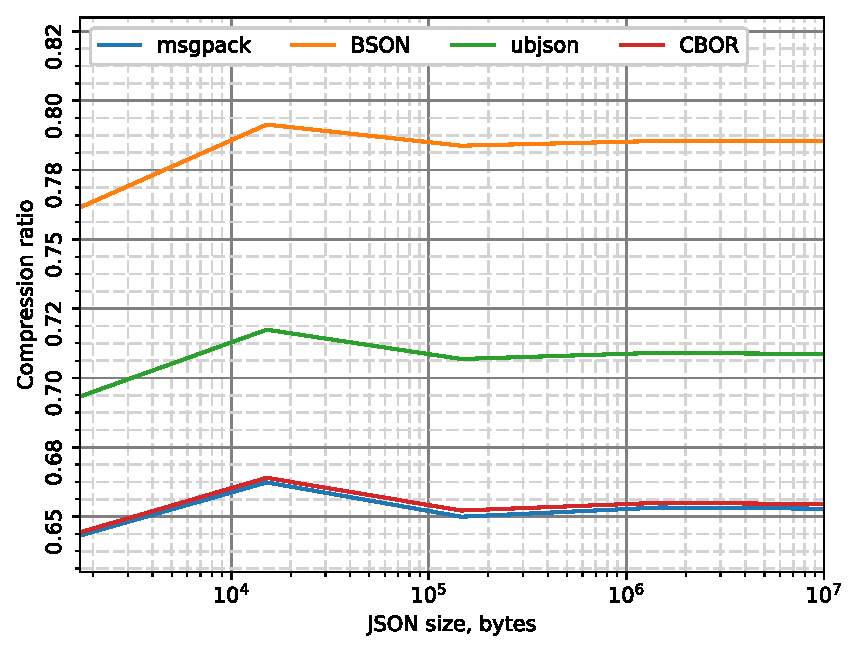
\includegraphics[width=0.7\textwidth]{ch-3/json-compession}
	\caption{Степень сжатия как функция размера файла JSON}
	\label{fig:json-compress}
\end{figure}


Затем была получена зависимость скорости упаковки/распаковки от размера файла JSON. Результаты показаны на рис.\cref{fig: json-pack} и\cref{fig: json-unpack}. Как видно, для всех рассмотренных библиотек эта зависимость линейная. Библиотека CBOR показала лучшее время как для упаковки, так и для распаковки.
Следующим шагом было тестирование производительности библиотек CBOR, написанных на разных языках программирования. Произошло 1000 циклов упаковки/распаковки; размер исходного файла JSON был 15\,МБ. Результаты тестирования представлены в таблице~\cref{tab:cbor}.

\begin{figure}[!ht]
	\centering
	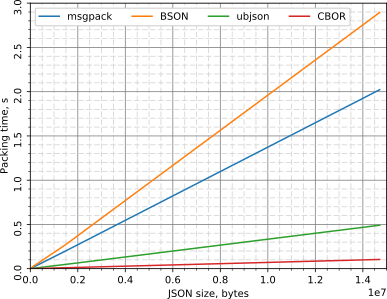
\includegraphics[width=0.7\textwidth]{ch-3/json-pack}
	\caption{Время упаковки в зависимости от размера файла JSON}
	\label{fig:json-pack}
\end{figure}

\begin{figure}[!ht]
	\centering
	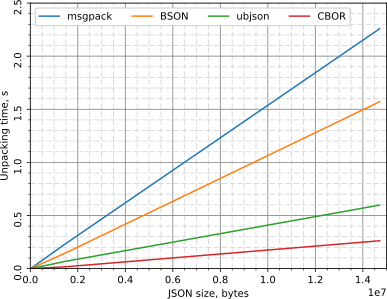
\includegraphics[width=0.7\textwidth]{ch-3/json-unpack}
	\caption{Время распаковки как функция размера файла JSON}
	\label{fig:json-unpack}
\end{figure}

\begin{table}[!htb]
\centering
\caption{Пропускная способность при использовании библиотек CBOR}
\label{tab:cbor}
	\begin{IEEEeqnarraybox} [\IEEEeqnarraystrutmode \IEEEeqnarraystrutsizeadd{2pt}{0pt}]{x/s/Vx/r/v/r/x}
	\IEEEeqnarraydblrulerowcut \\%
	%
	&&&& \IEEEeqnarraymulticol{3}{t}{Пропускная способность, Мбит/с} & \\
	%
	& \hfill \raisebox{-3pt} [0pt] [0pt]{Библиотека} \hfill && \IEEEeqnarraymulticol{5}{h}{}%
	
	\IEEEeqnarraystrutsize{0pt}{0pt} \\
	
	&&&& \hfill \raisebox{-1pt}[0pt][0pt]{Упаковка} \hfill &&
	\hfill \raisebox{-1pt}[0pt][0pt]{Распаковка} \hfill &
	\IEEEeqnarraystrutsizeadd{0pt}{2pt} \\
	%
	\IEEEeqnarraydblrulerowcut \\
	& Python 3.5.2 CBOR &&& 112.73 && 19.13 & \\
	& Python 3.5.2 CBOR2 &&& 7.59 && 4.30 & \\
	& C libcbor (GCC 6.2.0 20161005) &&& 244.13 && 273.07 & \\
	& JavaScript cbor (Chrome 56.0.2924.87) &&& 76.19 && 100.21 & \\
	\IEEEeqnarraydblrulerowcut \\
	\end{IEEEeqnarraybox}
\end{table}
%
\paragraph{Оценка производительности протоколов очереди сообщений}

Рисунок~\cref{fig:qm-bandwidth} показывает зависимость пропускной способности от размера сообщения. Для каждого метода было передано один миллион сообщений, и используется межпроцессное взаимодействие. По результатам анализа можно сделать вывод, что наиболее рациональный размер сообщения составляет от \SI{1}{\kilo\byte} до \SI{100}{\kilo\byte}.
Библиотеки~NanoMsg и ZeroMQ показали лучшую производительность. NanoMsg был выбран в качестве основного протокола передачи сообщений в рассматриваемой распределенной системе ЧПУ. Основные причины этого решения - лучшая совместимость с POSIX и более гибкий API.

В таблице\cref{tab: nanomsg} показаны результаты измерения пропускной способности протокола NanoMsg для различных сетевых подключений. Все тесты были написаны на Python, где размер сообщения \SI{1}{\kilo\byte}, и в каждом тесте был отправлено один миллион сообщений.

\begin{table}[!htb]
\centering
\caption{Пропускная способность при использовании протокола NanoMsg}
\label{tab:nanomsg}
	\begin{IEEEeqnarraybox} [\IEEEeqnarraystrutmode \IEEEeqnarraystrutsizeadd{2pt}{0pt}]{x/u/Vx/r/v/r/x}
	\IEEEeqnarraydblrulerowcut \\%
	%
	&&&& \IEEEeqnarraymulticol{3}{t}{Пропускная способность, Мбит/с} & \\
	%
	& \hfill \raisebox{-3pt}[0pt][0pt]{Библиотека} \hfill && \IEEEeqnarraymulticol{5}{h}{}%
	
	\IEEEeqnarraystrutsize{0pt}{0pt} \\
	
	&&&& \hfill \raisebox{-1pt}[0pt][0pt]{Nanomsg PUBSUB} \hfill &&
	\hfill \raisebox{-1pt}[0pt][0pt]{Nanomsg BUS} \hfill &
	\IEEEeqnarraystrutsizeadd{0pt}{2pt} \\
	%
	\IEEEeqnarraydblrulerowcut \\
	& Беспроводное соединение &&& 5.93 && 7.34 & \\
	& Кабельное соединение &&& 880.74 && 880.38 & \\
	& Облачное соединение &&& 15.18 && 14.98 & \\
	\IEEEeqnarraydblrulerowcut \\
	\end{IEEEeqnarraybox}
\end{table}


\begin{figure}[!htb]
	\centering
	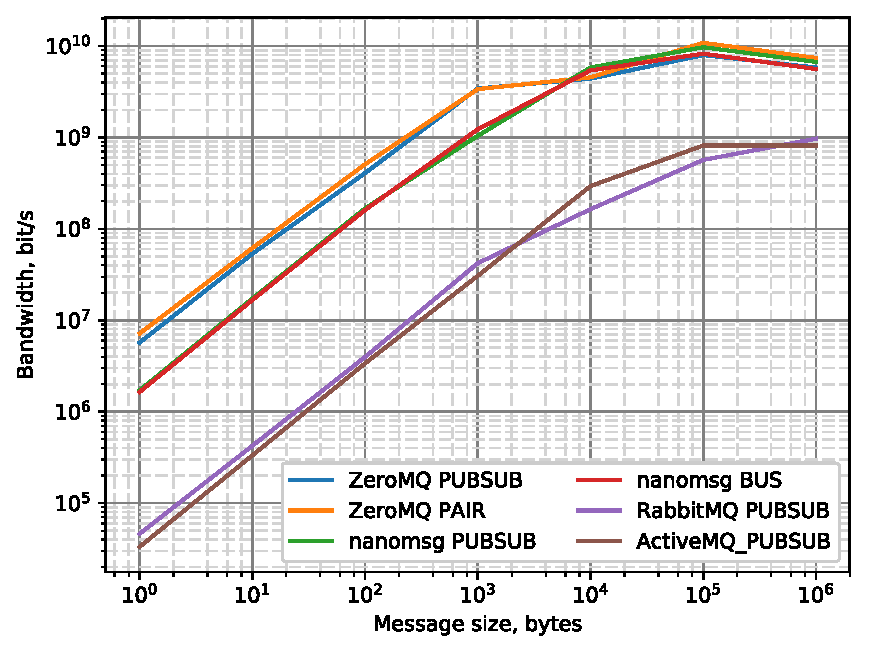
\includegraphics[width=0.9\textwidth]{ch-3/qm-bandwidth}
	\caption{Пропускная способность протоколов очереди сообщений в зависимости от размера сообщения}
	\label{fig:qm-bandwidth}
\end{figure}

\paragraph{Общая оценка производительности}

Чтобы дать общую оценку производительности протокола очереди сообщений, предлагается использовать формулу для средней полосы пропускания~\cref{eq:example}.

\begin{equation}
\begin{split}
	\label{eq:example}
	\mathcal{B}_a = \frac{\mathcal{M}}{t}
	= \frac{\mathcal{M}}{t_p + t_t + t_u}
	= \frac{\mathcal{M}}
	{\mathcal{M} / \mathcal{S}_p + 
		\gamma\mathcal{M} / \mathcal{B}_t + 
		\mathcal{M} / \mathcal{S}_u} = \\
	= \frac{\mathcal{M}}
	{\frac{\mathcal{M}_(\mathcal{B}_t\mathcal{S}_u) +
			\gamma
			\mathcal{M}(\mathcal{S}_p\mathcal{S}_u) +
			\mathcal{M}(\mathcal{S}_p\mathcal{B}_t)} 
		{\mathcal{S}_p\mathcal{B}_t\mathcal{S}_u}
	}
	=\frac{\mathcal{S}_p\mathcal{B}_t\mathcal{S}_u}
	{\mathcal{B}_t\mathcal{S}_u + \gamma\mathcal{S}_p\mathcal{S}_u + \mathcal{S}_p\mathcal{B}_t}\,,
\end{split}
\end{equation}

\noindent где ${\mathcal{M}}$ "--- размер сообщения, $t$ "--- общее время между двумя точками, $t_p$ "--- время упаковки, $t_t$ "--- время передачи, $t_u$ "--- время распаковки, $\mathcal{S}_p$ "--- скорость упаковки данных JSON, $\mathcal{S}_u$ "--- скорость распаковки данных JSON, $\mathcal{B}_t$ "--- пропускная способность очереди сообщений, $\gamma$ "--- степень сжатия JSON.

Часто библиотеки Python демонстрируют производительность, примерно равную производительности библиотек C. Это связано с тем, что эти библиотеки являются просто оболочками библиотек C. В этом случае использование библиотек Python предпочтительнее из-за более простого синтаксиса языка программирования Python. Однако рассматриваемые библиотеки Python не показали достаточной производительности, поэтому очевидно, что для реализации серверной части была выбрана библиотека C. При реализации клиентской части использовалась библиотека JS, так как это единственный вариант реализации программ в браузере.

В таблице~\cref{tab:res} показаны результаты расчетов. Расчеты показывают, что средняя полоса пропускания описанного канала связи находится в диапазоне от \SI{6}{\percent} (наихудший случай, упаковка/распаковка требуется на обеих конечных точках) до \SI{145}{\percent} (лучший случай, упаковка/распаковка вообще не требуется, обе конечные точки используют двоичные данные JSON, что подразумевает возможность сжатия сообщений из-за того, что двоичный формат JSON занимает меньше места по сравнению с текстовым JSON).

\begin{table}[!htb]
\centering
\caption{Пропускная способность, кабельное соединение, $\gamma=0,65$}
\label{tab:res}
	\begin{IEEEeqnarraybox} [\IEEEeqnarraystrutmode \IEEEeqnarraystrutsizeadd{2pt}{0pt}]{x/u/Vx/r/v/r/v/r/x/}
	\IEEEeqnarraydblrulerowcut \\
	
	& \hfill %\raisebox{0pt}[0pt][0pt]{Отношение $\mathcal{S}_u / \mathcal{S}$}
	\hfill && \IEEEeqnarraymulticol{0}{h}{}%
	\IEEEeqnarraystrutsize{0pt}{0pt} \\
	
	&&&& \hfill \raisebox{0pt}[0pt][0pt]{Библиотека JS} \hfill &&
	     \hfill \raisebox{0pt}[0pt][0pt]{Библиотека C} \hfill &&
	     \hfill \raisebox{0pt}[0pt][0pt]{Без распаковки} \hfill &
	\IEEEeqnarraystrutsizeadd{0pt}{2pt} \\
	%
	\IEEEeqnarraydblrulerowcut \\
	
	& Библиотека JS &&& n/a \rlap{\textsuperscript{1}} && {57.06} && 70.94 & \\
	& &&& &&{(6.22\,\%)} && (7.60\,\%) & \\
	
	& Библиотека  C &&& 67.50 && 117.70 && 203.18 & \\
	& &&& (7.24\,\%) && (12.62 \,\%) && (21.78 \, \%) & \\
	
	& Без упаковки &&& 93.31 && 227.27 && {1354.98} & \\
	& &&& (10.00\,\%) && (24.37\,\%) && {(145.28\,\%)} & \\
	%
	\IEEEeqnarraydblrulerowcut \\
	& \IEEEeqnarraymulticol{9}{s}{\scriptsize\textsuperscript{1} Cвязь между клиентами не реализована в рассматриваемом сценарии.}%
	\end{IEEEeqnarraybox}
\end{table}

\subsection{Методика оценка качества сигнала при беспроводном соединении модулей}

Наиболее узким местом в рассматриваемой информационной модели является передача данных по беспроводному каналу в условиях промышленного производства. Поэтому в данном разделе будет рассмотрена методика оценки качество соединения при использовании модулей беспроводной связи, в частности оценено влияние факторов производственной среды, которые могут привести к ухудшению связи и способов их устранения. В производстве присутствуют факторы, способные повлиять на помехозащищенность беспроводного сигнала. Поэтому проводятся различные исследования влияния производственной среды на беспроводной сигнал и определяются критерии его оценки. Например, шведские исследователи оценили влияние электромагнитного шума в цехах для различных диапазонов частот беспроводного сигнала~\cite{6525614, 5475862}. В ходе исследования они определили профиль снижения мощности в различных производственных помещениях с разными уровнями отражения и поглощения сигнала. Аналогичные исследования проводились также в Пекинском университете Цзяотун~\cite{Li2019}, где анализировались амплитудно-временные характеристики электромагнитных шумов на частотах 315, 433 и \SI{916}{\mega\hertz}, возникающих во время сварочных работ.
	
Также в работе~\cite{Girs2013DesignOC} описывается установка для измерения параметров беспроводного сигнала в диапазоне~\SI{2,4}{\giga\hertz}, а также методика измерения. Используя эту установку, учёные получили зависимость между стабильностью беспроводного сигнала и временем, необходимым для передачи стандартного пакета IEEE 802.15.4. В статье~\cite{8308609} рассматривается проблема шумового загрязнения в диапазоне~\SI{2,4}{\giga\hertz} другими сетями и источниками помех. Предложена математическая модель электромагнитного шума в этом диапазоне, которую можно использовать для предварительной оценки помехозащищенности производственных помещений.

Производство обычно рассматривается как иерархическая система, состоящая из уровней, как показано на~\cref{ch-3/fig-1}. На каждом уровне есть элементы сетевой инфраструктуры, обеспечивающие как горизонтальную, так и вертикальную передачу данных.
При этом типы используемых компьютерных сетей различаются на разных уровнях. Это происходит из-за того, что в зависимости от положения в иерархической системе выдвигаются различные требования к скорости передачи данных, безопасности, ширине канала, топологии, надежности и энергоэффективности. Более того, различные компьютерные сети могут сосуществовать на одном уровне в зависимости от выполняемых задач. Поэтому сетевая инфраструктура предприятия является гибридной.

\begin{figure*} [tb]
	\centering
	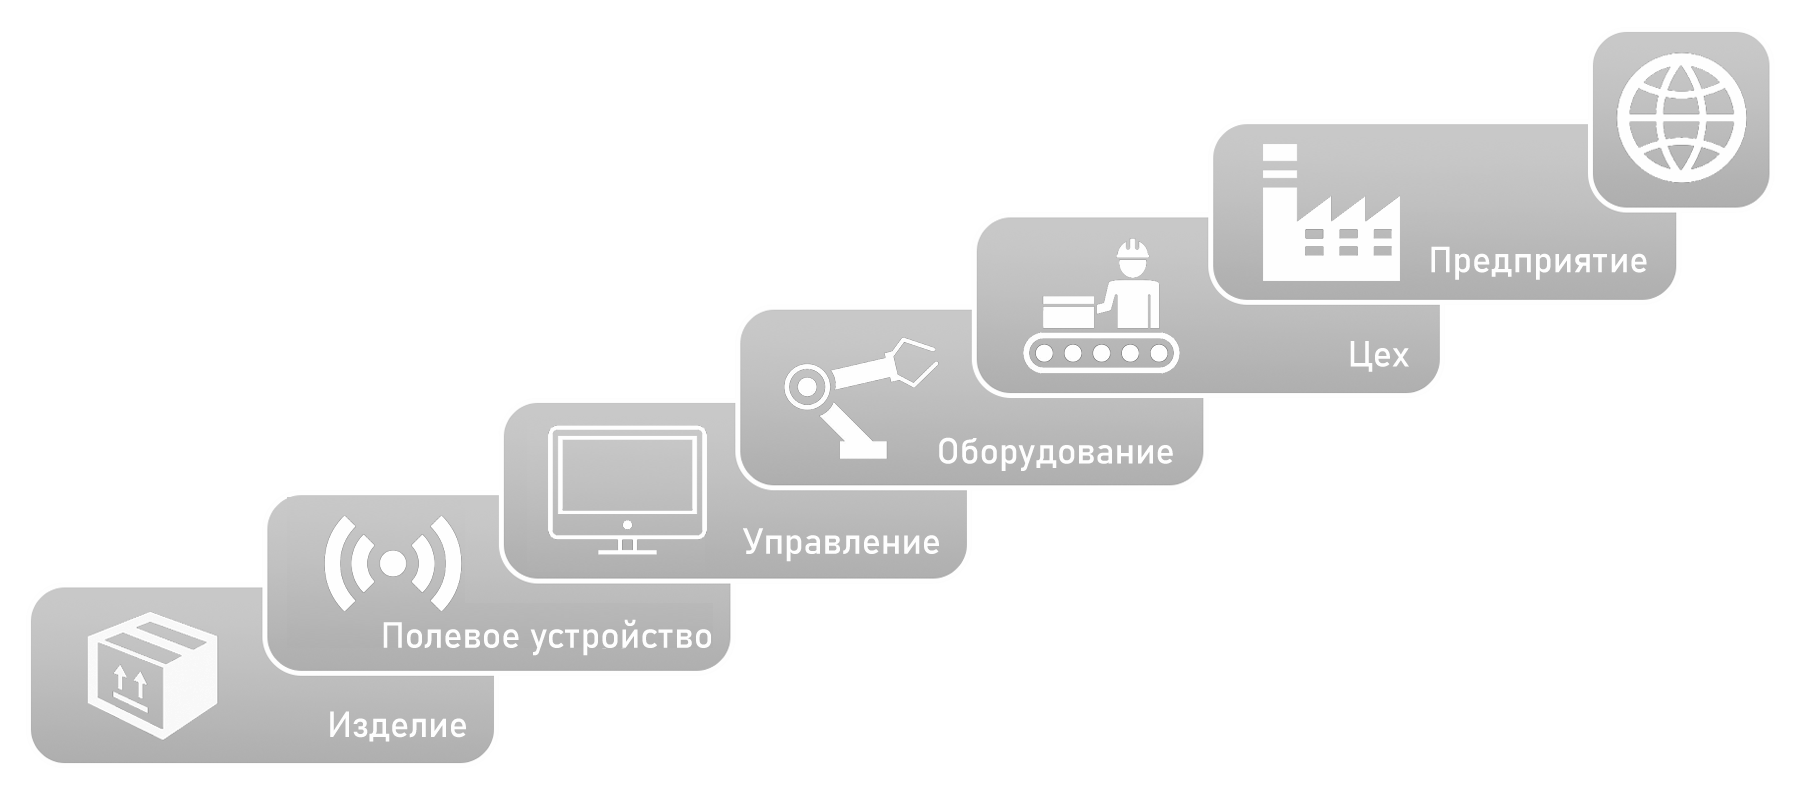
\includegraphics[width=0.9\linewidth]{ch-3/fig-1-ru}
	\caption{Уровни производственной системы}
	\label{ch-3/fig-1}
\end{figure*}

Беспроводные персональные вычислительные сети используются на уровнях системы управления, оборудования, производственной ячейки, цеха и, реже, в случае малых предприятий, на уровне всего предприятия. WPAN имеют широкое покрытие и применимы в производственной среде благодаря активной поддержке комитета IEEE (Институт инженеров по электротехнике и электронике). Это привело к появлению ряда технологий, охватываемых набором стандартов IEEE 802.15.4, включая хорошо известные технологии, такие как Bluetooth, ZigBee и Thread.

Одновременно стремительно растет аппаратная база. В настоящее время на рынке представлен большой выбор микросхем и готовых плат, поддерживающих сразу несколько технологий WPAN. Несмотря на изначально небольшую дальность передачи сигнала, использование сетки топология позволяет достичь практически неограниченного диапазона. Также стоит отметить возможность построения WPAN со стеком TCP/IP, что удобно при работе с другими сетями.

К недостаткам WPAN можно отнести частотные диапазоны, в которых работают эти сети: \SI{868}{\mega\hertz}, \SI{915}{\mega\hertz} и \SI{2,4}{\giga\hertz}. В России они не лицензированы, но имеют ограничения по мощности передатчика~\cite{freq}. Эти диапазоны называются <<частотами ISM>>.\footnote{Сокр. от англ. \textit{Industrial, Scientific, Medical}.} Как следует из названия, большое количество оборудования работает в диапазонах, которые могут создавать помехи сети~\cite{750064, 6209430}.

На производственной площадке существует множество факторов, которые могут ослабить и исказить беспроводной сигнал. Выявление этих аспектов перед развертыванием беспроводной сети является обязательной процедурой. Рисунок~\cref{ch-3/fig-2} представляет классификацию негативных факторов. Некоторые из этих факторов можно определить заранее уже на этапе разработки компоновки оборудования и агрегатов. Например, тип среды может определяться функциональным назначением производственного помещения. Зная окончательную компоновку блоков, можно определить, где офисные сети Wi-Fi~2,4\,ГГц будут пересекаться с промышленной беспроводной сетью. Учитывая это, можно вносить коррективы, чтобы повысить помехозащищенность сети.

\begin{figure*}[ht]
	\centering
	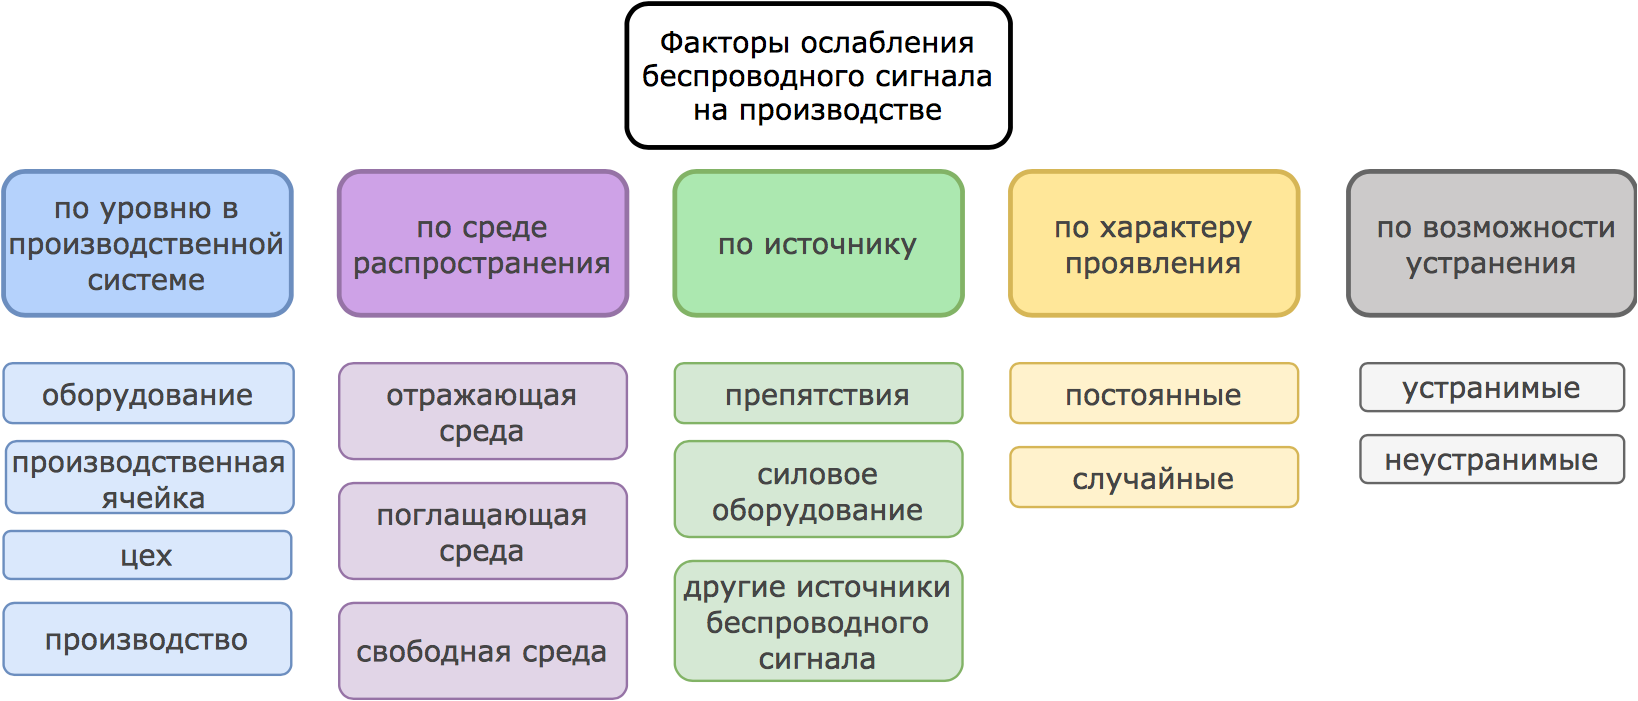
\includegraphics[width=\linewidth]{ch-3/fig-2-ru}
	\caption{Классификация производственных факторов, влияющих на прохождение радиосигнала}
	\label{ch-3/fig-2}
\end{figure*}

Однако новой беспроводной сети на уже существующей производственной площадке в настоящее время является более актуальной задачей. Кроме того, для получения достаточно точной картины измерения следует проводить непосредственно на предприятии. Для определения качества сигнала используются различные характеристики. Они включают профиль ослабления мощности, амплитудные и временные характеристики, отношение сигнал/шум~\cite{6133782} и т.\,д. К сожалению, значений этих параметров требует использования дорогостоящих инструментов "--- анализатора спектра, вектора анализатор цепей и специальные антенны. А квалификационные требования к человеку, производящему измерения, очень высоки.

В предлагаемой методике используется индикатор уровня принимаемого сигнала (RSSI). Его главное преимущество "--- встроенная поддержка практически на любом сетевом оборудовании, включая аппаратную платформу, используемую в эксперименте. Это означает, что можно получить значение RSSI от приемника без использования дополнительного измерительного оборудования. Однако RSSI нельзя использовать напрямую для измерения качества беспроводного сигнала, поскольку этот параметр может содержать значительный компонент помех. Таким образом, сильные помехи могут привести к потере пакетов при увеличении значения RSSI~\cite{8211460}.

Одновременно рассчитывается параметр $RSSI_T$, основанный на характеристиках антенн приемника и передатчика, а также с учётом частоты беспроводного сигнала и опорного параметра затухания~\cref{eq-1, eq-2, eq-3}:

\begin{equation}
	RSSI_T = A-10 \mu\log (d),
	\label{eq-1}
\end{equation}

\noindent где $d$ "--- расстояние от источника, м; $\mu$ "--- показатель ослабления, $\mu = 2$;

\begin{equation}
	A = P_{out} + G_{tx} + G_{rx} -FSPL,
	\label{eq-2}
\end{equation}

\noindent где $P_{out}$ "--- выходная мощность передатчика, дБм; $G_{tx}$ "--- усиление исходной антенны, дБи; $G_{rx}$ "--- усиление антенны приемника, дБи; $FSPL$ "--- потери на трассе в свободном пространстве, дБ;

\begin{equation}
	FSPL = 10 \log (d) +20 \log (f) +20 \log (4 \pi/c),
	\label{eq-3}
\end{equation}

\noindent где $f$ "--- частота, Гц; $c = 299792458$ м/с.

Поэтому в предлагаемом методе используется отклонение $\Delta RSSI$, полученное как разница между измеренным значением $RSSI_P$ и теоретическим значением $RSSI_T$~ \cref{eq-4}.

\begin{equation}
	\Delta RSSI = RSSI_T-RSSI_P
	\label{eq-4}
\end{equation}

Тем не менее, при проектировании сети, особенно в случае применения ячеистой топологии, сначала определяется расположение узлов в помещении. Следовательно, можно перейти от отклонения $\Delta RSSI$ к максимальному расстоянию между узлами~$D_{max}$~\cref{eq-5}, более удобному параметру для рассматриваемой задачи. Сигнал со значением RSSI менее~-80\,дБм считается слабым~\cite{mob_sig}. На основе этого утверждения и~\cref{eq-4} можно рассчитать$RSSI_T$~\cref{eq-6} на определенном расстоянии от передатчика с учетом среднего отклонения$\Delta RSSI$, на который влияют факторы конкретной производственной среды~\cref{eq-7}.

\begin{equation}
	D_{max} = 10^\frac{A-RSSI_T}{10 \mu}
	\label{eq-5}
\end{equation}

\begin{equation}
	RSSI_T = -80-\overline{{\mathit \Delta} RSSI}
	\label{eq-6}
\end{equation}

\begin{equation}
	\overline{{\mathit \Delta} RSSI} = \frac1n \sum_{\substack{0 < i < n}}{\mathit\Delta} RSSI_i,
	\label{eq-7}
\end{equation}

\noindent где $n$ "--- количество измерений. В этом случае $n = 25$.

\paragraph{План эксперимента}

Эксперимент проводился для определения существенных факторов, ослабляющих беспроводной сигнал в производственной среде. Для этого необходимо было собрать набор экспериментальных данных и оценить помехозащищенность WPAN под влиянием заданных факторов в соответствии с разработанной методикой.
Измерения были получены с использованием экспериментальной установки, показанной на~\cref{ch-3/fig-3}.

\begin{figure} [ht]
	\centering
	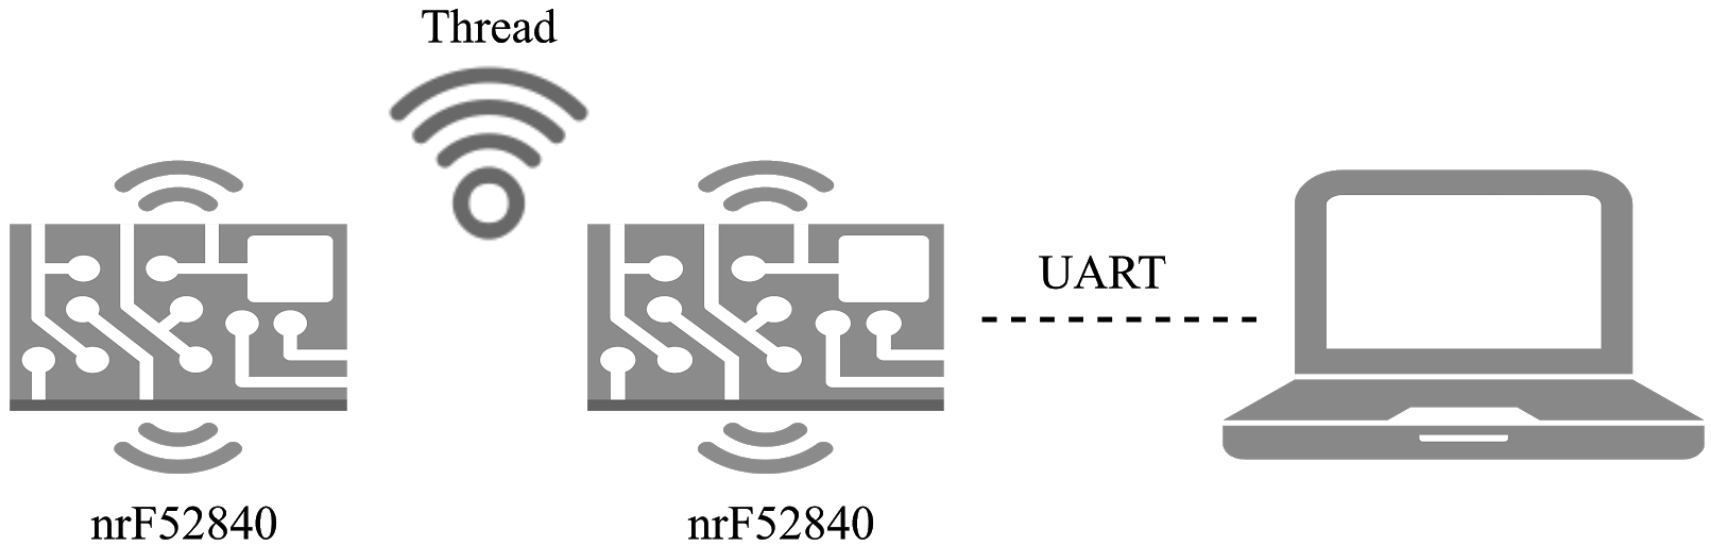
\includegraphics[width=\linewidth]{ch-3/fig-3}
	\caption{Экспериментальная установка}
	\label{ch-3/fig-3}
\end{figure}

Установка состоит из двух плат на базе микросхемы nRF52840\footnote{Электронный ресурс: {\url{https://wiki.makerdiary.com/nrf52840-mdk-usb-dongle/}} (дата обращения: 16.07.2020).}, которые действуют как приемник и передатчик. На плате установлена чип-антенна ACA-2012-A1-CC-S.\footnote{Электронный ресурс: \url{https://www.endrich.com/fm/2/ACA-2012-A1-CC-S.pdf} (дата обращения 23.02.2020).}
%параметры которой указаны в таблице~\cref{tab-1}.
Кроме того, для регистрации данных используется персональный компьютер. Персональный компьютер подключен к приемнику через интерфейс универсального асинхронного приемника-передатчика (UART) для получения измеренных значений RSSI. Внутри WPAN сообщение передается по протоколу Thread.\footnote{Электронный ресурс: {\url{https://openthread.io}} (дата обращения: 20.05.2020).}

Эксперимент проводился на производственных площадях компании <<Лар Технологии>>, специализирующейся на разработке технологического оборудования. Влияние каждого из следующих факторов разного типа, выбранных в соответствии с классификацией в~\cref{ch-3/fig-2}, изучалось отдельно.

\begin{itemize}
\item склад металлопроката;\footnote{Как фактор отражающей среды.}
\item силовое оборудование:
	\begin{itemize}
		\item асинхронный двигатель;
		\item шаговый двигатель;
		\item сварочный аппарат;
	\end{itemize}
\item толстостенная стальная труба (толщина стенки~\SI{20}{\milli\meter}) как фактор препятствия;
\item сети (Wi-Fi и ZigBee).
\end{itemize}

Значения RSSI под воздействием сетей~\SI{2,4}{\giga\hertz} были зафиксированы в многоквартирном доме, так как их не было в производственных помещениях. Также были получены измерения на открытом воздухе без влияния перечисленных факторов. Эксперимент проводился в диапазоне от 0,5 до \SI{24,5}{\meter} с шагом \SI{1}{\meter}. На каждом шаге выполнялась серия измерений в течение одной минуты с периодом~\SI{1}{\second}.

\paragraph{Результаты экспериментов.}

%\begin{table}[!h]
%	\centering
%	\caption{Спецификация чип-антенны ACA-2012-A1-CC-S} \vspace{4pt}
%	\label{tab-1}
%	\begin{tabularx}{\linewidth}{XX}
%		\toprule
%		\textbf{Параметр} & \textbf{Значение} \\
%		\midrule
%		Диапазон частот (МГц) & 2400--2483 \\
%		Коэффициент стоячей волны &$<$3,0\\
%		Поляризация & линейная \\
%		Входное сопротивление (Ом) & 50 \\
%		Коэффициент усиления (дБи) & 1,72 \\
%		Размеры (мм) & 2,0 $\times$ 1,2 $\times$ 0,55\\
%		\bottomrule
%	\end{tabularx}
%\end{table}

По мере увеличения расстояния между приемником и передатчиком значение RSSI уменьшается, что можно объяснить явлением потерь на пути распространения. В этом случае значение RSSI уменьшается логарифмически в зависимости от расстояния~\cref{eq-1}. Это происходит в соответствии с законом сохранения энергии. Поскольку волна передает энергию и распространяется сферически, энергия с увеличением расстояния распределяется по увеличивающейся площади поверхности сферы.~\footnote{Электронный ресурс: {\tiny\url{http://asupro.com/gps-gsm/means-identification/automatic/linear-circular-polarization-rfid-system.html}} (дата обращения: 09.05.2020).} Рисунок~\cref{ch-3/fig-4a} показывает график, отражающий теоретическую кривую значений RSSI, полученных в соответствии с~\cref{eq-1}, и зависимость между RSSI и расстоянием при измерениях на открытом воздухе. Можно отметить, что кривые оказались похожими по форме. Однако есть небольшие отклонения RSSI, значения которых показаны в~\cref{ch-3/fig-4b}.

\begin{figure}[!htb]
	\centering
	\subfloat []{%
		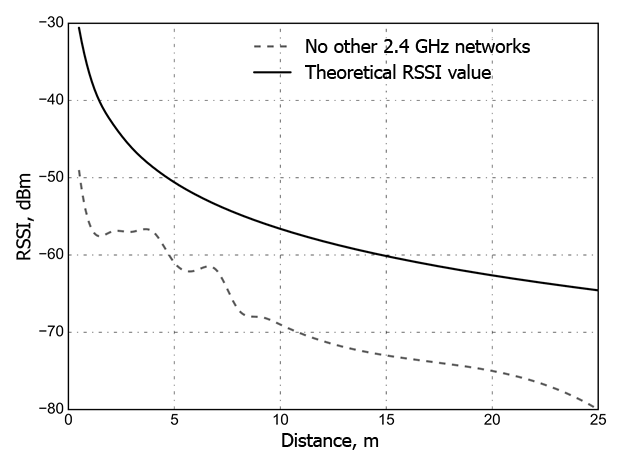
\includegraphics[clip, width=0.49\textwidth]{ch-3/fig-4a}%
		\label{ch-3/fig-4a}
	}
	\subfloat []{%
		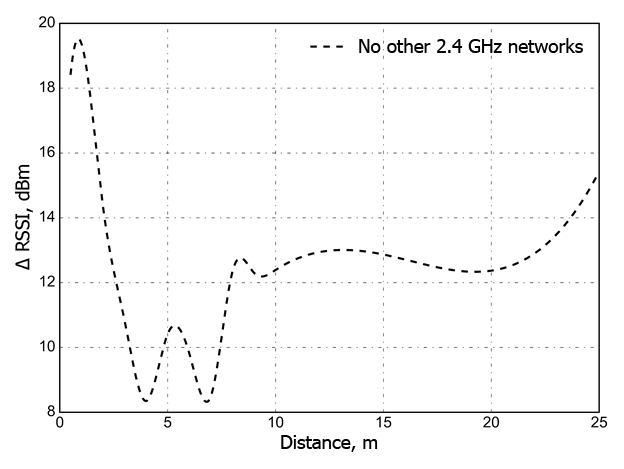
\includegraphics[clip, width=0.49\textwidth]{ch-3/fig-4b}%
		\label{ch-3/fig-4b}
	}
	\caption[Влияние характеристик приемника и передатчика на $RSSI$ и отклонение $RSSI$ от теоретического значения]{Влияние характеристик приемника и передатчика на: $RSSI$ (\textit{а}) и отклонение $RSSI$ от теоретического значения (\textit{б})}
\end{figure}

Одной из отличительных характеристик промышленного производства является тип среды, по которой распространяется беспроводной сигнал. Производство чаще всего характеризуется отражающей средой, за некоторыми исключениями, например, целлюлозно-бумажные и деревообрабатывающие предприятия, где преобладает поглощающая среда. Распространение сигнала в отражающей среде подвержено эффекту многолучевого распространения~\cite{7433518}. В результате принимаются не только прямые, но и отраженные лучи, что приводит к колебаниям амплитуды, фазы и угла входного сигнала. На рисунке~\cref{ch-3/fig-5} показаны графики $RSSI$ и $\Delta RSSI$ в зависимости от расстояния соответственно. Графики показывают значительные колебания, вызванные указанным выше эффектом.

\begin{figure} [tb]
	\subfloat []{%
		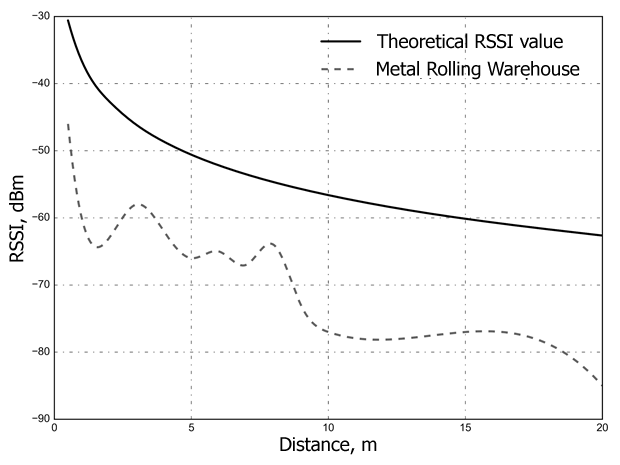
\includegraphics[clip, width=0.49\textwidth]{ch-3/fig-5a}%
		\label{ch-3/fig-5a}
	}
	\subfloat []{%
		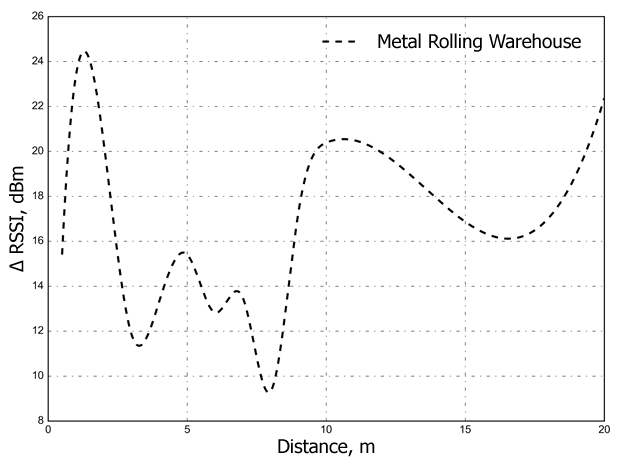
\includegraphics[clip, width=0.49\textwidth]{ch-3/fig-5b}%
		\label{ch-3/fig-5b}
	}
	\caption[Влияние отражающей среды на: $RSSI$ и отклонение $RSSI$ от теоретического значения]{Влияние отражающей среды на: $RSSI$(\textit{а}) и отклонение $RSSI$ от теоретического значения (\textit{б})}
	\label{ch-3/fig-5}
\end{figure}

Препятствия, встречающиеся на пути распространения сигнала, имеют аналогичный эффект. Кроме того, могут возникать явления дифракции (на поверхностях с резкими неровностями) и рассеяния (на шероховатых поверхностях). Стены между цехами и производственными ячейками могут отражать сигнал из-за наличия арматуры и, с другой стороны, поглощать его из-за звукоизоляции. Более того, в производственных помещениях бывают ситуации, когда приемник или передатчик может располагаться только за определенным препятствием или внутри бокса. \cref{ch-3/fig-6} показывает данные для этого случая. Полученный результат аналогичен показанному на~\cref{ch-3/fig-5}; однако отклонение $RSSI$ больше, поскольку препятствие окружало приемник и находилось в непосредственной близости от него.

\begin{figure} [tb]
	\subfloat []{%
		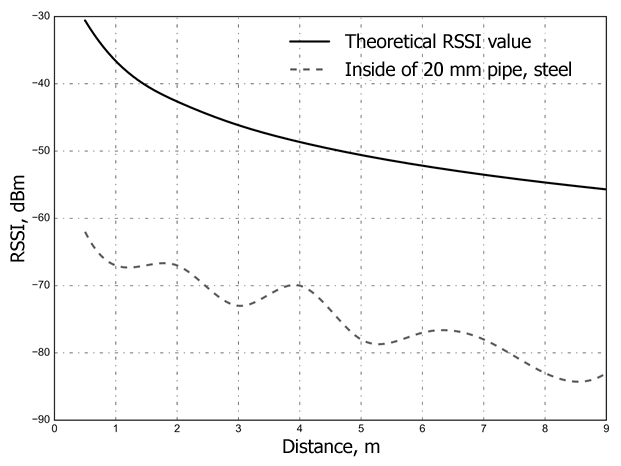
\includegraphics[clip, width=0.49\textwidth]{ch-3/fig-6a}%
		\label{ch-3/fig-6a}
	}
	\subfloat []{%
		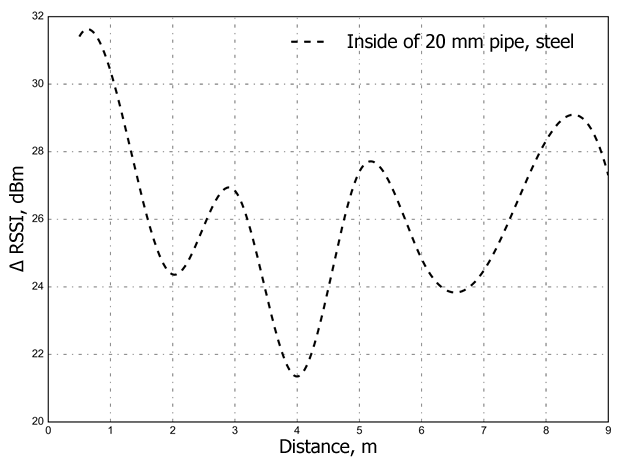
\includegraphics[clip, width=0.49\textwidth]{ch-3/fig-6b}%
		\label{ch-3/fig-6b}
	}
	\caption[Влияние препятствий в производственном помещении на: RSSI и отклонение RSSI от теоретического значения)]{Влияние препятствий в производственном помещении на: $RSSI$ (\textit{а}) и отклонение RSSI от теоретического значения (\textit{б})}
	\label{ch-3/fig-6}
\end{figure}

Поскольку инфраструктура производственной сети отличается неоднородностью, вполне вероятно, что несколько беспроводных сетей будут работать одновременно в одном и том же диапазоне частот. В этом случае могут возникать интерференции, накладываются когерентные волны, что приводит к увеличению или уменьшению результирующей амплитуды. Этот эффект может быть особенно заметен, когда устройства работают на одном канале, что типично для диапазона~\SI{2,4}{\giga \hertz}, где сети Wi-Fi, Bluetooth, ZigBee и Thread пересекаются~\cite{016461}. Полученные графики в~\cref{ch-3/fig-7} показывают значительное влияние этого фактора.

\begin{figure} [htb]
	\subfloat []{%
	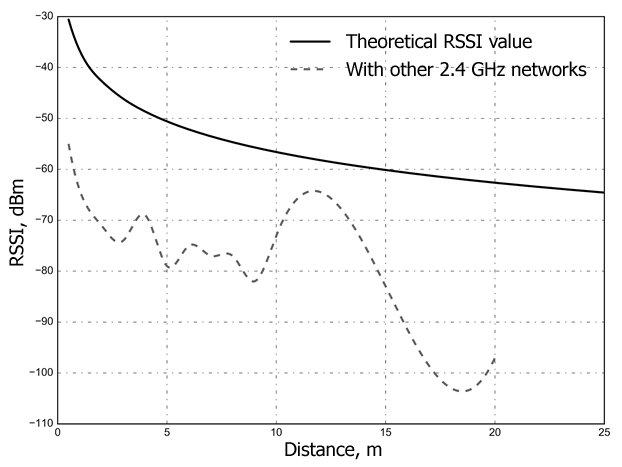
\includegraphics[clip, width=0.49\textwidth]{ch-3/fig-7a}%
	\label{ch-3/fig-7a}
	}
	\subfloat []{%
	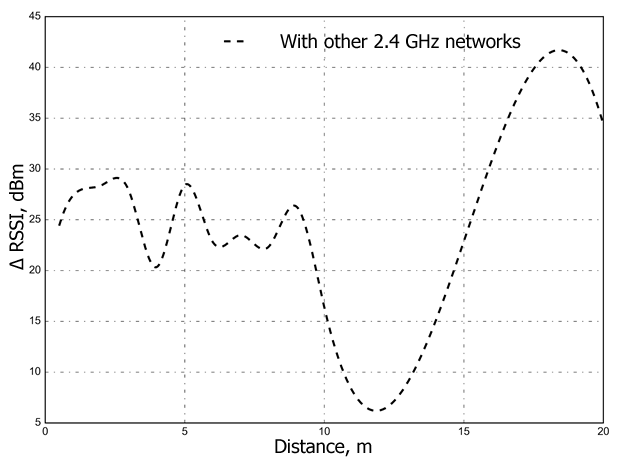
\includegraphics[clip, width=0.49\textwidth]{ch-3/fig-7b}%
	\label{ch-3/fig-7b}
	}
	\caption[Влияние соседних сетей~\SI{2,4}{\giga \hertz} на: отклонение RSSI и $RSSI$ от теоретического значения]
	{Влияние соседних сетей~\SI{2,4}{\giga \hertz} на: отклонение RSSI (\textit{а}) и $RSSI$ от теоретического значения (\textit{б})}
	\label{ch-3/fig-7}
\end{figure}

Большое количество силового оборудования, расположенного в помещении цеха, может искажать передаваемый беспроводной сигнал и вызывать помехи. Чаще всего это наблюдается при распространении импульсного сигнала по линиям электропередачи оборудования. Это происходит потому, что при формировании фронта амплитуда сигнала изменяется с большой скоростью, что приводит к появлению большого количества высокочастотных гармоник в спектре сигнала. В случае рассматриваемого в эксперименте шагового двигателя управление осуществляется с помощью широтно-импульсной модуляции (ШИМ). Графики на рисункек~\cref{ch-3/fig-8} показывают искажение беспроводного сигнала. Для асинхронного двигателя (рисунок~\cref{ch-3/fig-9}) сильных колебаний не наблюдалось, так как управление производилось без использования преобразователя частоты. Сварочный аппарат показал один из худших показателей (рисунокк~\cref{ch-3/fig-10}), так как при переключении транзисторных ключей инвертора в процессе сварки на фронтах импульсов происходит большое количество кратковременных переходных процессов в виде затухающих высокочастотных колебания.\footnote{Электронный ресурс: {\tiny\url{https://303421.selcdn.ru/soel-upload/clouds/1/iblock/e03/e036d5c6f8c271c7ebbf44799619f068/201002052.pdf}} (дата обращения 01.05.2020).}

\begin{figure} [htb]
	\subfloat []{%
	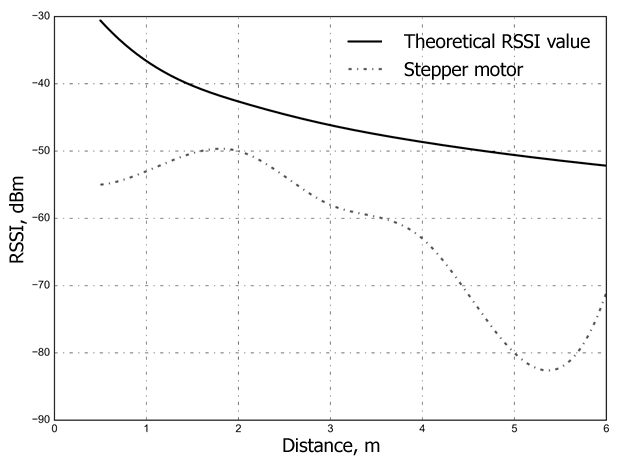
\includegraphics[clip, width=0.49\textwidth]{ch-3/fig-8a}%
	\label{ch-3/fig-8a}
	}
	\subfloat []{%
	\includegraphics[clip, width=0.49\textwidth]{ch-3/fig-8b}%
	\label{ch-3/fig-8b}
	}
	\caption[Влияние исправного шагового двигателя на: отклонение $RSSI$ и $RSSI$ от теоретического значения]
	{Влияние исправного шагового двигателя на: отклонение $RSSI$ (\textit{а}) и $RSSI$ от теоретического значения (\textit{б})}
	\label{ch-3/fig-8}
\end{figure}

\begin{figure} [htb]
	\subfloat []{%
	\includegraphics[clip, width=0.49\textwidth]{ch-3/fig-9a}%
	\label{ch-3/fig-9a}
	}
	\subfloat []{%
	\includegraphics[clip, width=0.49\textwidth]{ch-3/fig-9b}%
	\label{ch-3/fig-9b}
	}
	\caption[Влияние работающего асинхронного двигателя на: отклонение $RSSI$ и $RSSI$ от теоретического значения]
	{Влияние работающего асинхронного двигателя на: отклонение $RSSI$ (\textit{а}) и $RSSI$ от теоретического значения (\textit{б})}
	\label{ch-3/fig-9}
\end{figure}

\begin{figure} [htb]
	\subfloat []{%
	\includegraphics[clip, width=0.49\textwidth]{ch-3/fig-10a}%
	\label{ch-3/fig-10a}
	}
	\subfloat []{%
	\includegraphics[clip, width=0.49\textwidth]{ch-3/fig-10b}%
	\label{ch-3/fig-10b}
	}
	\caption[Влияние работающего сварочного аппарата на: отклонение $RSSI$ и $RSSI$ от теоретического значения]
	{Влияние работающего сварочного аппарата на: отклонение $RSSI$ (\textit{а}) и $RSSI$ от теоретического значения (\textit{б})}
	\label{ch-3/fig-10}
\end{figure}

В таблице~\cref{tab-2} приводятся результаты серии экспериментов. Наихудший результат был получен в эксперименте, когда ствольная коробка была помещена в толстостенную стальную трубу. Это означает, что этого приемника следует избегать или его следует располагать не дальше~6,85\,м от передатчика. Наилучшие результаты были показаны при измерении RSSI в свободной среде.

Имеется небольшое отклонение от теоретического значения. Из-за некоторых аппаратных особенностей антенны, которые не учитывались в расчетах, и среднего теоретического значения показателя затухания. Следует отметить, что возможность организации WPAN на основе топологии ячеистой сети позволяет нейтрализовать негативные эффекты за счет плотного расположения сетевых узлов, согласно рассчитанному~$D_{max}$.

\begin{table}[!htb]
\centering
\caption{Влияние производственных факторов на помехозащищенность беспроводных персональных сетей (WPAN)} \vspace{4pt}
\label{tab-2}
\begin{threeparttable}
\begin{tabularx}{\linewidth}{@{} lrrr}
	\toprule
	\textbf{Факторы} &
	{\small $\Delta R$} \tnote{1} &
	{\small $\Delta R_{max}$} \tnote{2} &
	{\small $D_{max}$} \tnote{3} \\
	\midrule
	Свободная среда без других сетей \SI{2,4}{\giga\hertz} & 12,37 & 18,82 & 34,22 \\
	Асинхронный двигатель & 12.69 & 19.37 & 33.99 \\
	Отражающая среда (склад металла) & 16.33 & 23.39 & 22.54 \\
	Шаговый двигатель & 17.51 & 29.41 & 19.67 \\
	Сварочный аппарат & 21.11 & 34.35 & 13.01 \\
	Среда с шумом от других сетей \SI{2,4}{\giga\hertz} & 25,03 & 32,37 & 8,27 \\
	Экранирование толстостенной стальной трубой & 26,67 & 34,41 & 6,85 \\
	\bottomrule
\end{tabularx}
\begin{tablenotes} \footnotesize
	\item [1] Средняя ошибка $\Delta RSSI$, дБм
	\item [2] Максимальная ошибка $\Delta RSSI_{max}$, дБм
	\item [3] Максимальное расстояние между передатчиками, м
\end{tablenotes}
\end{threeparttable}
\end{table}

\section{Выводы по главе 3}

Данная глава посвящена исследвованию методик информационного взаимодействия компонентов системы управления модульным оборудованием. В главе представлена архитектура модульной децентрализованной системы управления, в основе которой лежит распределённый реестр, содержащий все данные о составе и структуре единицы модульного оборудования, а также комплекса модульных установвок, если их несколько. Каждая единица в данном случае представляется узлом иерархической базы данных в формате JSON. Отдельные параметры называются слотами, в слоты записываются конкретные параметры модулей. Каждая единица оборудовани характеризуется коммуникационными параметрами, выполняемыми функциями и возвращаемыми значениями с допустимым диапазоном для проверки. При этом в основе каждой установки находится шасси, которое в информационном плане агрегирует информацию о модулях и осуществляет первичную автоналадку всех систем. Под выполняемыми функциями модулей подразумеваются G и M и прочие коды ISO-7bit коды, которые могут быть реализованы средствами того или иного модуля. 

С технической точки зрения модули и шасси (как частный случай с точки зрения алгоритма управления) взаимодействуют по протоколу Thread. Поддерживается как прододное подключене,так и беспроводное подключение. Thread позволяет организовать сеть ячеистой топологией с автообнаружением узлов. Данные между узлами сети передаются через безброкерную очередь сообщений NanoMsg, формат передачи данных "--- уже упомянутый JSON, упакованный в бинорный вид.  

Для определения максимальной пропускной способности ячеистой сети было произведено исследование различных прикладный программных библиотек. Было показано, что лучшее время упаковки/распаковки и степень сжатия данных JSON продемонстрировала библиотека CBOR. Было определено, что степень сжатия не зависит от объёма исходного файла JSON. По результатам анализа также был сделан вывод, что наиболее подходящий размер сообщения "--- от 1 КБ до 100 КБ. Были произведены расчёты общей производительности связки протокола NanoMsg и упаковщика CBOR. Расчеты показали, что полоса пропускания этого канала данных находится в диапазоне от \SI{6}{\percent} до \SI{145}{\percent} от средней пропускной способности сети при использовании сокетов Raw TCP, что можно считать хорошим результатом для этого типа программного обеспечения.

Также был проведён ряд экспериментов, которые определяют помехоустойчивость беспроводного способа передачи данных в производственной среде. Предложен метод оценки помехозащищенности сетей на основе параметра $RSSI$. Выявлены факторы ослабления беспроводного сигнала и рассчитаны значения помехоустойчивости на реальной производственной площадке.

Учитывая полученные данные, можно сделать вывод, что многие производственные факторы оказывают существенное влияние на качество сигнала в беспроводной сети. Однако воздействие недостаточно велико, чтобы полностью отказываться от использования этой технологии. Более того, влияние многих факторов может быть уменьшено за счет применения топологии ячеистой сети и плотного расположения приемников и передатчиков. Стоит подчеркнуть важность проведения соответствующих измерений для каждого конкретного производства, поскольку это обеспечивает эффективное размещение приемников и передатчиков в производственных помещениях.

\FloatBarrier           % Глава 3
\chapter*{Заключение}                       % Заголовок
\addcontentsline{toc}{chapter}{Заключение}  % Добавляем его в оглавление

%% Согласно ГОСТ Р 7.0.11-2011:
%% 5.3.3 В заключении диссертации излагают итоги выполненного исследования, рекомендации, перспективы дальнейшей разработки темы.
%% 9.2.3 В заключении автореферата диссертации излагают итоги данного исследования, рекомендации и перспективы дальнейшей разработки темы.
%% Поэтому имеет смысл сделать эту часть общей и загрузить из одного файла в автореферат и в диссертацию:

Основные результаты работы заключаются в следующем.
%% Согласно ГОСТ Р 7.0.11-2011:
%% 5.3.3 В заключении диссертации излагают итоги выполненного исследования, рекомендации, перспективы дальнейшей разработки темы.
%% 9.2.3 В заключении автореферата диссертации излагают итоги данного исследования, рекомендации и перспективы дальнейшей разработки темы.

Значимость полученных в диссертационной работе результатов подчеркивается возможностью интеграции разработанных методик, подходов и алгоритмов в систему автоматизированного проектирования модульного технологического оборудования. Предложенные рекомендации по созданию узлов и агрегатов, а также блоков управления модульным технологическим оборудованием упростят его разработку и применение в условиях единичного и мелкосерийного производства.  В ходе исследования получены следующие основные теоретические и практические результаты:

\begin{enumerate}
  \item Предложена универсальная конструкция переналаживаемого модульного оборудования, состоящая из универсального координатного шасси с подвижной кареткой; модулей, определяющих основную операцию выполняемую оборудованием и устанавливаемых на подвесе каретки шасси посредством электромагнитного крепления; и модульного блока управления, реализующего алгоритм числового программного управления. 
  \item Разработано алгоритмическое и программно-техническое обеспечение модульного блока управления, включающее в себя набор программно-аппаратных средств для реализации децентрализованного сетевого взаимодействия модулей в проводной и беспроводной среде передачи данных и программное обеспечение для автоматической реконфигурации единицы модульного оборудования, позволяющее снизить трудоёмкость переналадки.  
  \item Разработана методика унификации модулей с электромагнитным креплением, включающая в себя способ определения параметров унификации и их ограничений и способ формирования параметрического ряда на основании сформулированных ограничений.
  \item Предложен критерий целесообразности применения модульного оборудования, основанный на анализе групповых технологических процессов, позволяющий оценить  перспективы использования модульного оборудования для типовых технологических процессов, используемых на предприятии.
  \item Разработана методика оптимизации комплекта модульного оборудования, включающая в себя способ расчёта весовых коэффициентов целевой функции оптимизации и алгоритм двухкритериальной оптимизации, основанный на теории нормирования и дискретно-событийном методе.
  \item На основании методики оптимизации комплекта модульного оборудования разработано программное обеспечение и проведен численный эксперимент, показавший повышение производительности производства группы изделий на~\SI{18}{\percent}.
  \item Для тестирования предложенной конструкции модульного оборудования, а также методик и алгоритмов работы с ним создан прототип модульной технологической платформы.
\end{enumerate}

Таким образом, на основании полученных результатов, цель данного диссертационного исследования по разработке модульного технологического оборудования для условий единичного и мелкосерийного производства можно считать достигнутой.

Полученные результаты соответствуют пункту 6 <<Разработка, исследование и внедрение новых видов технологического оборудования для изготовления деталей, сборки, регулировки, контроля и испытаний приборов>> и пункту 7 <<Разработка и внедрение новых методов и средств механизации, автоматизации, роботизации приборостроительного производства, обеспечивающих повышение производительности, снижение трудоемкости и повышение экономичности производства>> паспорта специальности 05.11.14 "--- <<Технология приборостроения>>.

%И какая-нибудь заключающая фраза.

%Последний параграф может включать благодарности.  В заключение автор
%выражает благодарность и большую признательность научному руководителю
%Иванову~И.\,И. за поддержку, помощь, обсуждение результатов и~научное
%руководство. Также автор благодарит Сидорова~А.\,А. и~Петрова~Б.\,Б.
%за помощь в~работе с~образцами, Рабиновича~В.\,В. за предоставленные
%образцы и~обсуждение результатов, Занудятину~Г.\,Г. и авторов шаблона
%*Russian-Phd-LaTeX-Dissertation-Template* за~помощь в оформлении
%диссертации. Автор также благодарит много разных людей
%и~всех, кто сделал настоящую работу автора возможной.
      % Заключение
\chapter*{Список сокращений и условных обозначений} % Заголовок
\addcontentsline{toc}{chapter}{Список сокращений и условных обозначений}  % Добавляем его в оглавление
% при наличии уравнений в левой колонке значение параметра leftmargin приходится подбирать вручную

\begin{description}[align=right,leftmargin=3.5cm]
\item[ЧПУ] числовое программное управление
\item[ПО] программное обеспечение
\item[МИП] малое инновационное предприятие
\item[КИМ] контрольно-измерительная машина 
\item[АСУ ТП] автоматизированная система управления технологическими процессами
\item[АС] агрегатный станок
\item[НТИ] национальная технологическая инициатива
\item[НТЦ] научно-технологических центров
\item[ПЛК] программируемый логический контроллер

\item[RMS] Reconfigurable Machine Tools
\item[OEM] Original Equipment Manufacturer

\end{description}
        % Список сокращений и условных обозначений
\chapter*{Словарь терминов}             % Заголовок
\addcontentsline{toc}{chapter}{Словарь терминов}  % Добавляем его в оглавление

%\textbf{TeX} : Cистема компьютерной вёрстки, разработанная американским профессором информатики Дональдом Кнутом

%\textbf{панграмма} : Короткий текст, использующий все или почти все буквы алфавита

\textbf{Экспонирование} : облучение актиничным излучением (излучение, которое оказывает фотографическое действие на светочувствительный материал) светочувствительного слоя через фотошаблон или с помощью управляемого луча.

\textbf{Фоторезист} : светочувствительный материал, изменяющий свои свойства (прежде всего "--- растворимость) под воздействием актиничного излучения. 

\textbf{Ламинирование} : наложение полимера на подложку с последующей прикаткой и охлаждением для получения армированных многослойных изделий, состоящих из нескольких слоев разнородных материалов.

\textbf{Проявление} : обработка экспонированной пленки фоторезиста с целью удаления необлученных участков для создания рельефного изображения

\textbf{Экструзия} : получение изделий из пластмасс и резиновых смесей в экструдере (машина для пластикации материалов и придания им формы путем продавливания через экструзионную головку)

\textbf{Экструзия заготовок} : Формообразование заготовок непрерывным или периодическим выдавливанием пластического материала через канал формующего инструмента "--- головку 

\textbf{Пайка готовым припоем} : способ пайки, при котором используется заранее приготовленный припой. В качестве припоя может использоваться металлический (полностью расплавляемый) или композиционный припой. В композиционном припое помимо металлической основы содержится тугоплавкий наполнитель (порошки, волокна, сетки), который сам не плавится, а при плавлении металла припоя образует разветвленную сеть капилляров, удерживающих под действием капиллярных сил его жидкую часть в зазоре между соединяемыми деталями (ГОСТ 17325-79).
      % Словарь терминов
\include{Dissertation/references}      % Список литературы
\include{Dissertation/lists}           % Списки таблиц и изображений (иллюстративный материал)

\setcounter{totalchapter}{\value{chapter}} % Подсчёт количества глав

%%% Настройки для приложений
\appendix
% Оформление заголовков приложений ближе к ГОСТ:
\setlength{\midchapskip}{20pt}
\renewcommand*{\afterchapternum}{\par\nobreak\vskip \midchapskip}
\renewcommand\thechapter{\Asbuk{chapter}} % Чтобы приложения русскими буквами нумеровались

\chapter{Тексты публикаций}\label{app:A}


\clearpage
%\refstepcounter{chapter}
%\addcontentsline{toc}{appendix}{\protect\chapternumberline{\thechapter}Чертёж детали}

\includepdf[pages=-, pagecommand={}]{Dissertation/papers/performance-eval-2017.pdf}
\includepdf[pages=-, pagecommand={}]{Dissertation/papers/modular-eq-arch-2017.pdf}
\includepdf[pages=-, pagecommand={}]{Dissertation/papers/microservices-2017.pdf}
\includepdf[pages=-, pagecommand={}]{Dissertation/papers/etherium-2018.pdf}
\includepdf[pages=-, pagecommand={}]{Dissertation/papers/mesh-2018.pdf}
\includepdf[pages=-, pagecommand={}]{Dissertation/papers/noise-2020.pdf}

        % Приложения

\setcounter{totalappendix}{\value{chapter}} % Подсчёт количества приложений

\end{document}
